%%%%%%%%%%%%%%%%%%%%%%%%%%%%%%%%%%%%%%%%%
%  My documentation report
%  Objetive: Explain what I did and how, so someone can continue with the investigation
%
% Important note:
% Chapter heading images should have a 2:1 width:height ratio,
% e.g. 920px width and 460px height.
%
%%%%%%%%%%%%%%%%%%%%%%%%%%%%%%%%%%%%%%%%%

%----------------------------------------------------------------------------------------
%	PACKAGES AND OTHER DOCUMENT CONFIGURATIONS
%----------------------------------------------------------------------------------------

\documentclass[11pt,fleqn]{book} % Default font size and left-justified equations

\usepackage[top=3cm,bottom=3cm,left=3.2cm,right=3.2cm,headsep=10pt,letterpaper]{geometry} % Page margins
\usepackage[dvipsnames]{xcolor}
\usepackage{lipsum} % Required for specifying colors by name

% Font Settings
\usepackage{avant} % Use the Avantgarde font for headings
%\usepackage{times} % Use the Times font for headings
\usepackage{mathptmx} % Use the Adobe Times Roman as the default text font together with math symbols from the Symbol, Chancery and Computer Modern fonts

\usepackage{microtype} % Slightly tweak font spacing for aesthetics
\usepackage[utf8]{inputenc} % Required for including letters with accents
\usepackage[T1]{fontenc} % Use 8-bit encoding that has 256 glyphs

\usepackage[french]{varioref}
\usepackage[french]{babel}

\usepackage{wrapfig}
\usepackage{listings}
\usepackage{multicol}
\usepackage{multirow}
\usepackage{colortbl}
\usepackage{booktabs}
\newcommand{\tabitem}{~~\llap{\textbullet}~~}
\usepackage{hyperref}
\usepackage{qrcode}
\usepackage{soul}
\usepackage{tabto}
\usepackage{multienum}


\definecolor{deepblue}{rgb}{0.0,0.0,0.5}
\definecolor{deepred}{rgb}{0.6,0,0}
\definecolor{deepgreen}{rgb}{0,0.5,0}
\definecolor{ocre}{RGB}{51,102,0} 
\definecolor{lightgray}{RGB}{229,229,229} 
\definecolor{palerod}{RGB}{238,232,170}

\newcommand\pythonstyle{\lstset{
language=Python,
basicstyle=\ttfamily\footnotesize,
morekeywords={self},              % Add keywords here
frame=tb,                         % Any extra options here
showstringspaces=false
}}

\definecolor{backcolour}{rgb}{0.95,0.95,0.92}

\newcommand\termctyle{\lstset{
frame=tb,                         % Any extra options here
showstringspaces=false
}}


% Python environment
\lstnewenvironment{python}[1][]
{
\pythonstyle
\lstset{#1}
}
{}

\lstnewenvironment{termc}[1][]
{
\lstset{#1}
}
{}


% RFC
\newcommand\rfc[1]{\href{http://www.ietf.org/rfc/rfc#1.txt}{\textcolor{blue}{RFC #1}\index{RFC #1}}}
\newcommand\pfunction[2]{\texttt{#2}\index{Module Python!#1!#2}}

% boot.py

\newcommand\glos[1]{\gls{#1}\index{#1}}
\newcommand\pprog[2]{\href{https://github.com/ltn22/PLIDObis/blob/master/#2/#1}{\texttt{#1}}\index{Programmes Python!#1}}
\newcommand\lprog[2]{\href{https://github.com/ltn22/PLIDObis/blob/master/#2/#1}{\texttt{#1}}\index{Programmes micro-python!#1}}

% QUESTION

\usepackage[most]{tcolorbox}
\usepackage{ifthen}

\provideboolean{Response}\setboolean{Response}{true}

\newcommand{\Correct}[1]{\ifthenelse{\boolean{Response}}{#1}{\textbf{#1}}}
\newcommand{\Wrong}[1]{\ifthenelse{\boolean{Response}}{#1}{\textcolor{black!20}{#1}}}

\newwrite\tempfile
\immediate\openout\tempfile=questions.tex


\newtcbtheorem[auto counter,number within=section]{theo}%
  {Question}{fonttitle=\bfseries\upshape, 
     arc=0mm, colback=blue!5!white,colframe=blue!75!black}{Question}
     
\newcommand\Question[3]{
\begin{theo}{#1}{summation}
#2
\immediate\write\tempfile{\noexpand\textbf{Question \thetcbcounter {} page \thepage} {} }
\immediate\write\tempfile{\unexpanded{#2}\noexpand\vspace{1em}\noexpand\newline}
\immediate\write\tempfile{\noexpand\textit{\unexpanded{#3}}\noexpand\newline\noexpand\newline}

\end{theo}
}

% MATHS PACKAGE
\usepackage{amsmath,tikz}
\usetikzlibrary{matrix}
\newcommand*{\horzbar}{\rule[0.05ex]{2.5ex}{0.5pt}}
\usepackage{calc}

% VERBATIM PACKAGE
\usepackage{verbatim}

\usepackage{tikz}

\usetikzlibrary{automata}
\usetikzlibrary[shadows]
\usetikzlibrary{shapes}
\usetikzlibrary[decorations.footprints] 
\usetikzlibrary{decorations.pathmorphing}
\usetikzlibrary{decorations.pathreplacing}
\usetikzlibrary{decorations.text}
\usetikzlibrary {arrows}
\usetikzlibrary{patterns}
\usetikzlibrary{calc}
\usetikzlibrary{external}

\usepackage{tikz-timing}

% Acronyms

\usepackage{makeidx}
\makeindex

\usepackage{acronym}

\let\oldac\ac
\renewcommand*{\ac}[1]{\oldac{#1}\index{#1}}

\newcommand\Index[1]{\textbf{#1}\index{#1}}

% Bibliography
\usepackage[style=alphabetic,sorting=nyt,sortcites=true,autopunct=true,babel=hyphen,hyperref=true,abbreviate=false,backref=true,backend=biber]{biblatex}
\addbibresource{bibliography.bib} % BibTeX bibliography file
\defbibheading{bibempty}{}

%----------------------------------------------------------------------------------------
%	VARIOUS REQUIRED PACKAGES
%----------------------------------------------------------------------------------------

\usepackage{titlesec} % Allows customization of titles

\usepackage{graphicx} % Required for including pictures
\graphicspath{{Pictures/}} % Specifies the directory where pictures are stored

\usepackage{lipsum} % Inserts dummy text

\usepackage{tikz} % Required for drawing custom shapes

\usepackage[french]{babel} % English language/hyphenation

\usepackage{enumitem} % Customize lists
\setlist{nolistsep} % Reduce spacing between bullet points and numbered lists

\usepackage{booktabs} % Required for nicer horizontal rules in tables

\usepackage{eso-pic} % Required for specifying an image background in the title page

%----------------------------------------------------------------------------------------
%	MAIN TABLE OF CONTENTS
%----------------------------------------------------------------------------------------

\usepackage{titletoc} % Required for manipulating the table of contents

\contentsmargin{0cm} % Removes the default margin
% Chapter text styling
\titlecontents{chapter}[1.25cm] % Indentation
{\addvspace{15pt}\large\sffamily\bfseries} % Spacing and font options for chapters
{\color{ocre!60}\contentslabel[\Large\thecontentslabel]{1.25cm}\color{ocre}} % Chapter number
{}  
{\color{ocre!60}\normalsize\sffamily\bfseries\;\titlerule*[.5pc]{.}\;\thecontentspage} % Page number
% Section text styling
\titlecontents{section}[1.25cm] % Indentation
{\addvspace{5pt}\sffamily\bfseries} % Spacing and font options for sections
{\contentslabel[\thecontentslabel]{1.25cm}} % Section number
{}
{\sffamily\hfill\color{black}\thecontentspage} % Page number
[]
% Subsection text styling
\titlecontents{subsection}[1.25cm] % Indentation
{\addvspace{1pt}\sffamily\small} % Spacing and font options for subsections
{\contentslabel[\thecontentslabel]{1.25cm}} % Subsection number
{}
{\sffamily\;\titlerule*[.5pc]{.}\;\thecontentspage} % Page number
[] 

%----------------------------------------------------------------------------------------
%	MINI TABLE OF CONTENTS IN CHAPTER HEADS
%----------------------------------------------------------------------------------------

% Section text styling
\titlecontents{lsection}[0em] % Indendating
{\footnotesize\sffamily} % Font settings
{}
{}
{}

% Subsection text styling
\titlecontents{lsubsection}[.5em] % Indentation
{\normalfont\footnotesize\sffamily} % Font settings
{}
{}
{}
 
%----------------------------------------------------------------------------------------
%	PAGE HEADERS
%----------------------------------------------------------------------------------------

\usepackage{fancyhdr} % Required for header and footer configuration

\pagestyle{fancy}
\renewcommand{\chaptermark}[1]{\markboth{\sffamily\normalsize\bfseries\chaptername\ \thechapter.\ #1}{}} % Chapter text font settings
\renewcommand{\sectionmark}[1]{\markright{\sffamily\normalsize\thesection\hspace{5pt}#1}{}} % Section text font settings
\fancyhf{} \fancyhead[LE,RO]{\sffamily\normalsize\thepage} % Font setting for the page number in the header
\fancyhead[LO]{\rightmark} % Print the nearest section name on the left side of odd pages
\fancyhead[RE]{\leftmark} % Print the current chapter name on the right side of even pages
\renewcommand{\headrulewidth}{0.5pt} % Width of the rule under the header
\addtolength{\headheight}{2.5pt} % Increase the spacing around the header slightly
\renewcommand{\footrulewidth}{0pt} % Removes the rule in the footer
\fancypagestyle{plain}{\fancyhead{}\renewcommand{\headrulewidth}{0pt}} % Style for when a plain pagestyle is specified

% Removes the header from odd empty pages at the end of chapters
\makeatletter
\renewcommand{\cleardoublepage}{
\clearpage\ifodd\c@page\else
\hbox{}
\vspace*{\fill}
\thispagestyle{empty}
\newpage
\fi}

%----------------------------------------------------------------------------------------
%	THEOREM STYLES
%----------------------------------------------------------------------------------------

\usepackage{amsmath,amsfonts,amssymb,amsthm} % For math equations, theorems, symbols, etc

\newcommand{\intoo}[2]{\mathopen{]}#1\,;#2\mathclose{[}}
\newcommand{\ud}{\mathop{\mathrm{{}d}}\mathopen{}}
\newcommand{\intff}[2]{\mathopen{[}#1\,;#2\mathclose{]}}
\newtheorem{notation}{Notation}[chapter]

%%%%%%%%%%%%%%%%%%%%%%%%%%%%%%%%%%%%%%%%%%%%%%%%%%%%%%%%%%%%%%%%%%%%%%%%%%%
%%%%%%%%%%%%%%%%%%%% dedicated to boxed/framed environements %%%%%%%%%%%%%%
%%%%%%%%%%%%%%%%%%%%%%%%%%%%%%%%%%%%%%%%%%%%%%%%%%%%%%%%%%%%%%%%%%%%%%%%%%%
\newtheoremstyle{ocrenumbox}% % Theorem style name
{0pt}% Space above
{0pt}% Space below
{\normalfont}% % Body font
{}% Indent amount
{\small\bf\sffamily\color{ocre}}% % Theorem head font
{\;}% Punctuation after theorem head
{0.25em}% Space after theorem head
{\small\sffamily\color{ocre}\thmname{#1}\nobreakspace\thmnumber{\@ifnotempty{#1}{}\@upn{#2}}% Theorem text (e.g. Theorem 2.1)
\thmnote{\nobreakspace\the\thm@notefont\sffamily\bfseries\color{black}---\nobreakspace#3.}} % Optional theorem note
\renewcommand{\qedsymbol}{$\blacksquare$}% Optional qed square

\newtheoremstyle{blacknumex}% Theorem style name
{5pt}% Space above
{5pt}% Space below
{\normalfont}% Body font
{} % Indent amount
{\small\bf\sffamily}% Theorem head font
{\;}% Punctuation after theorem head
{0.25em}% Space after theorem head
{\small\sffamily{\tiny\ensuremath{\blacksquare}}\nobreakspace\thmname{#1}\nobreakspace\thmnumber{\@ifnotempty{#1}{}\@upn{#2}}% Theorem text (e.g. Theorem 2.1)
\thmnote{\nobreakspace\the\thm@notefont\sffamily\bfseries---\nobreakspace#3.}}% Optional theorem note

\newtheoremstyle{blacknumbox} % Theorem style name
{0pt}% Space above
{0pt}% Space below
{\normalfont}% Body font
{}% Indent amount
{\small\bf\sffamily}% Theorem head font
{\;}% Punctuation after theorem head
{0.25em}% Space after theorem head
{\small\sffamily\thmname{#1}\nobreakspace\thmnumber{\@ifnotempty{#1}{}\@upn{#2}}% Theorem text (e.g. Theorem 2.1)
\thmnote{\nobreakspace\the\thm@notefont\sffamily\bfseries---\nobreakspace#3.}}% Optional theorem note

%%%%%%%%%%%%%%%%%%%%%%%%%%%%%%%%%%%%%%%%%%%%%%%%%%%%%%%%%%%%%%%%%%%%%%%%%%%
%%%%%%%%%%%%% dedicated to non-boxed/non-framed environements %%%%%%%%%%%%%
%%%%%%%%%%%%%%%%%%%%%%%%%%%%%%%%%%%%%%%%%%%%%%%%%%%%%%%%%%%%%%%%%%%%%%%%%%%
\newtheoremstyle{ocrenum}% % Theorem style name
{5pt}% Space above
{5pt}% Space below
{\normalfont}% % Body font
{}% Indent amount
{\small\bf\sffamily\color{ocre}}% % Theorem head font
{\;}% Punctuation after theorem head
{0.25em}% Space after theorem head
{\small\sffamily\color{ocre}\thmname{#1}\nobreakspace\thmnumber{\@ifnotempty{#1}{}\@upn{#2}}% Theorem text (e.g. Theorem 2.1)
\thmnote{\nobreakspace\the\thm@notefont\sffamily\bfseries\color{black}---\nobreakspace#3.}} % Optional theorem note
\renewcommand{\qedsymbol}{$\blacksquare$}% Optional qed square
\makeatother

% Defines the theorem text style for each type of theorem to one of the three styles above
\newcounter{dummy} 
\numberwithin{dummy}{section}
\theoremstyle{ocrenumbox}
\newtheorem{theoremeT}[dummy]{Theorem}
\newtheorem{problem}{Problem}[chapter]
\newtheorem{exerciseT}{Exercise}[chapter]
\theoremstyle{blacknumex}
\newtheorem{exampleT}{Example}[chapter]
\theoremstyle{blacknumbox}
\newtheorem{vocabulary}{Vocabulary}[chapter]
\newtheorem{definitionT}{Definition}[section]
\newtheorem{corollaryT}[dummy]{Corollary}
\theoremstyle{ocrenum}
\newtheorem{proposition}[dummy]{Proposition}

%----------------------------------------------------------------------------------------
%	DEFINITION OF COLORED BOXES
%----------------------------------------------------------------------------------------

\RequirePackage[framemethod=default]{mdframed} % Required for creating the theorem, definition, exercise and corollary boxes

% Theorem box
\newmdenv[skipabove=7pt,
skipbelow=7pt,
backgroundcolor=black!5,
linecolor=ocre,
innerleftmargin=5pt,
innerrightmargin=5pt,
innertopmargin=5pt,
leftmargin=0cm,
rightmargin=0cm,
innerbottommargin=5pt]{tBox}

% Exercise box	  
\newmdenv[skipabove=7pt,
skipbelow=7pt,
rightline=false,
leftline=true,
topline=false,
bottomline=false,
backgroundcolor=ocre!10,
linecolor=ocre,
innerleftmargin=5pt,
innerrightmargin=5pt,
innertopmargin=5pt,
innerbottommargin=5pt,
leftmargin=0cm,
rightmargin=0cm,
linewidth=4pt]{eBox}	

% Definition box
\newmdenv[skipabove=7pt,
skipbelow=7pt,
rightline=false,
leftline=true,
topline=false,
bottomline=false,
linecolor=ocre,
innerleftmargin=5pt,
innerrightmargin=5pt,
innertopmargin=0pt,
leftmargin=0cm,
rightmargin=0cm,
linewidth=4pt,
innerbottommargin=0pt]{dBox}	

% Corollary box
\newmdenv[skipabove=7pt,
skipbelow=7pt,
rightline=false,
leftline=true,
topline=false,
bottomline=false,
linecolor=gray,
backgroundcolor=black!5,
innerleftmargin=5pt,
innerrightmargin=5pt,
innertopmargin=5pt,
leftmargin=0cm,
rightmargin=0cm,
linewidth=4pt,
innerbottommargin=5pt]{cBox}

% Creates an environment for each type of theorem and assigns it a theorem text style from the "Theorem Styles" section above and a colored box from above
\newenvironment{theorem}{\begin{tBox}\begin{theoremeT}}{\end{theoremeT}\end{tBox}}
\newenvironment{exercise}{\begin{eBox}\begin{exerciseT}}{\hfill{\color{ocre}\tiny\ensuremath{\blacksquare}}\end{exerciseT}\end{eBox}}				  
\newenvironment{definition}{\begin{dBox}\begin{definitionT}}{\end{definitionT}\end{dBox}}	
\newenvironment{example}{\begin{exampleT}}{\hfill{\tiny\ensuremath{\blacksquare}}\end{exampleT}}		
\newenvironment{corollary}{\begin{cBox}\begin{corollaryT}}{\end{corollaryT}\end{cBox}}	

%----------------------------------------------------------------------------------------
%	REMARK ENVIRONMENT
%----------------------------------------------------------------------------------------

\newenvironment{remark}{\par\vspace{10pt}\small % Vertical white space above the remark and smaller font size
\begin{list}{}{
\leftmargin=35pt % Indentation on the left
\rightmargin=25pt}\item\ignorespaces % Indentation on the right
\makebox[-2.5pt]{\begin{tikzpicture}[overlay]
\node[draw=ocre!60,line width=1pt,circle,fill=ocre!25,font=\sffamily\bfseries,inner sep=2pt,outer sep=0pt] at (-15pt,0pt){\textcolor{ocre}{R}};\end{tikzpicture}} % Orange R in a circle
\advance\baselineskip -1pt}{\end{list}\vskip5pt} % Tighter line spacing and white space after remark

%----------------------------------------------------------------------------------------
%	SECTION NUMBERING IN THE MARGIN
%----------------------------------------------------------------------------------------

\makeatletter
\renewcommand{\@seccntformat}[1]{\llap{\textcolor{ocre}{\csname the#1\endcsname}\hspace{1em}}}                    
\renewcommand{\section}{\@startsection{section}{1}{\z@}
{-4ex \@plus -1ex \@minus -.4ex}
{1ex \@plus.2ex }
{\normalfont\large\sffamily\bfseries}}
\renewcommand{\subsection}{\@startsection {subsection}{2}{\z@}
{-3ex \@plus -0.1ex \@minus -.4ex}
{0.5ex \@plus.2ex }
{\normalfont\sffamily\bfseries}}
\renewcommand{\subsubsection}{\@startsection {subsubsection}{3}{\z@}
{-2ex \@plus -0.1ex \@minus -.2ex}
{.2ex \@plus.2ex }
{\normalfont\small\sffamily\bfseries}}                        
\renewcommand\paragraph{\@startsection{paragraph}{4}{\z@}
{-2ex \@plus-.2ex \@minus .2ex}
{.1ex}
{\normalfont\small\sffamily\bfseries}}

%----------------------------------------------------------------------------------------
%	HYPERLINKS IN THE DOCUMENTS
%----------------------------------------------------------------------------------------

% For an unclear reason, the package should be loaded now and not later
\usepackage{hyperref}
\hypersetup{hidelinks,backref=true,pagebackref=true,hyperindex=true,colorlinks=false,breaklinks=true,urlcolor= ocre,bookmarks=true,bookmarksopen=false,pdftitle={Title},pdfauthor={Author}}

%----------------------------------------------------------------------------------------
%	CHAPTER HEADINGS
%----------------------------------------------------------------------------------------

% The set-up below should be (sadly) manually adapted to the overall margin page septup controlled by the geometry package loaded in the main.tex document. It is possible to implement below the dimensions used in the goemetry package (top,bottom,left,right)... TO BE DONE

\newcommand{\thechapterimage}{}
\newcommand{\chapterimage}[1]{\renewcommand{\thechapterimage}{#1}}

% Numbered chapters with mini tableofcontents
\def\thechapter{\arabic{chapter}}
\def\@makechapterhead#1{
\thispagestyle{empty}
{\centering \normalfont\sffamily
\ifnum \c@secnumdepth >\m@ne
\if@mainmatter
\startcontents
\begin{tikzpicture}[remember picture,overlay]
\node at (current page.north west)
{\begin{tikzpicture}[remember picture,overlay]
\node[anchor=north west,inner sep=0pt] at (0,0) {\includegraphics[width=\paperwidth]{\thechapterimage}};
%%%%%%%%%%%%%%%%%%%%%%%%%%%%%%%%%%%%%%%%%%%%%%%%%%%%%%%%%%%%%%%%%%%%%%%%%%%%%%%%%%%%%
% Commenting the 3 lines below removes the small contents box in the chapter heading
%\fill[color=ocre!10!white,opacity=.6] (1cm,0) rectangle (8cm,-7cm);
%\node[anchor=north west] at (1.1cm,.35cm) {\parbox[t][8cm][t]{6.5cm}{\huge\bfseries\flushleft \printcontents{l}{1}{\setcounter{tocdepth}{2}}}};
\draw[anchor=west] (5cm,-9cm) node [rounded corners=20pt,fill=ocre!10!white,text opacity=1,draw=ocre,draw opacity=1,line width=1.5pt,fill opacity=.6,inner sep=12pt]{\huge\sffamily\bfseries\textcolor{black}{\thechapter. #1\strut\makebox[22cm]{}}};
%%%%%%%%%%%%%%%%%%%%%%%%%%%%%%%%%%%%%%%%%%%%%%%%%%%%%%%%%%%%%%%%%%%%%%%%%%%%%%%%%%%%%
\end{tikzpicture}};
\end{tikzpicture}}
\par\vspace*{230\p@}
\fi
\fi}

% Unnumbered chapters without mini tableofcontents (could be added though) 
\def\@makeschapterhead#1{
\thispagestyle{empty}
{\centering \normalfont\sffamily
\ifnum \c@secnumdepth >\m@ne
\if@mainmatter
\begin{tikzpicture}[remember picture,overlay]
\node at (current page.north west)
{\begin{tikzpicture}[remember picture,overlay]
\node[anchor=north west,inner sep=0pt] at (0,0) {\includegraphics[width=\paperwidth]{\thechapterimage}};
\draw[anchor=west] (5cm,-9cm) node [rounded corners=20pt,fill=ocre!10!white,fill opacity=.6,inner sep=12pt,text opacity=1,draw=ocre,draw opacity=1,line width=1.5pt]{\huge\sffamily\bfseries\textcolor{black}{#1\strut\makebox[22cm]{}}};
\end{tikzpicture}};
\end{tikzpicture}}
\par\vspace*{230\p@}
\fi
\fi
}
\makeatother % Insert the commands.tex file which contains the majority of the structure behind the template



\newcommand\pythonlst[2][]{
\lstinputlisting[language=Python, backgroundcolor=\color{palerod},   basicstyle=\footnotesize\ttfamily,
  keywordstyle=\bfseries\color{green!40!black},
  commentstyle=\itshape\color{purple!40!black},
  identifierstyle=\color{blue},
  stringstyle=\color{orange}, caption=#2,
  numbers=left, numberstyle=\tiny, stepnumber=2, numbersep=5pt, frame=single, #1] {Programs/#2}\index{Programmes Python!#2}
  }

\newcommand\pythonnxt[2][]{
\lstinputlisting[language=Python, backgroundcolor=\color{palerod},   basicstyle=\footnotesize\ttfamily,
  keywordstyle=\bfseries\color{green!40!black},
  commentstyle=\itshape\color{purple!40!black},
  identifierstyle=\color{blue},
  stringstyle=\color{orange},
  numbers=left, numberstyle=\tiny, stepnumber=2, numbersep=5pt, frame=single, #1] {Programs/#2}
  }
  
  
\newcommand\pycomlst[2][]{
\lstinputlisting[language=Python, backgroundcolor=\color{gray!10},   basicstyle=\footnotesize\ttfamily,
  keywordstyle=\bfseries\color{green!40!black},
  commentstyle=\itshape\color{purple!40!black},
  identifierstyle=\color{blue},
  stringstyle=\color{orange}, caption=#2,
  numbers=left, numberstyle=\tiny, stepnumber=2, numbersep=5pt, frame=single, #1] {Programs/#2}\index{Programmes micro-python!#2}
  }

\newcommand\pycomnxt[2][]{
\lstinputlisting[language=Python, backgroundcolor=\color{gray!10},   basicstyle=\footnotesize\ttfamily,
  keywordstyle=\bfseries\color{green!40!black},
  commentstyle=\itshape\color{purple!40!black},
  identifierstyle=\color{blue},
  stringstyle=\color{orange},
  numbers=left, numberstyle=\tiny, stepnumber=2, numbersep=5pt, frame=single, #1] {Programs/#2}
  }



\newcommand\Youtube[1]{\begin{tcolorbox}[colback=red!5,colframe=red!75!black,title=Youtube, width=3cm]\href{#1}{\qrcode{#1}}\end{tcolorbox}}




\begin{document}

\let\cleardoublepage\clearpage

%----------------------------------------------------------------------------------------
%	TITLE PAGE
%----------------------------------------------------------------------------------------

\begingroup
\thispagestyle{empty}
\AddToShipoutPicture*{\put(0,0){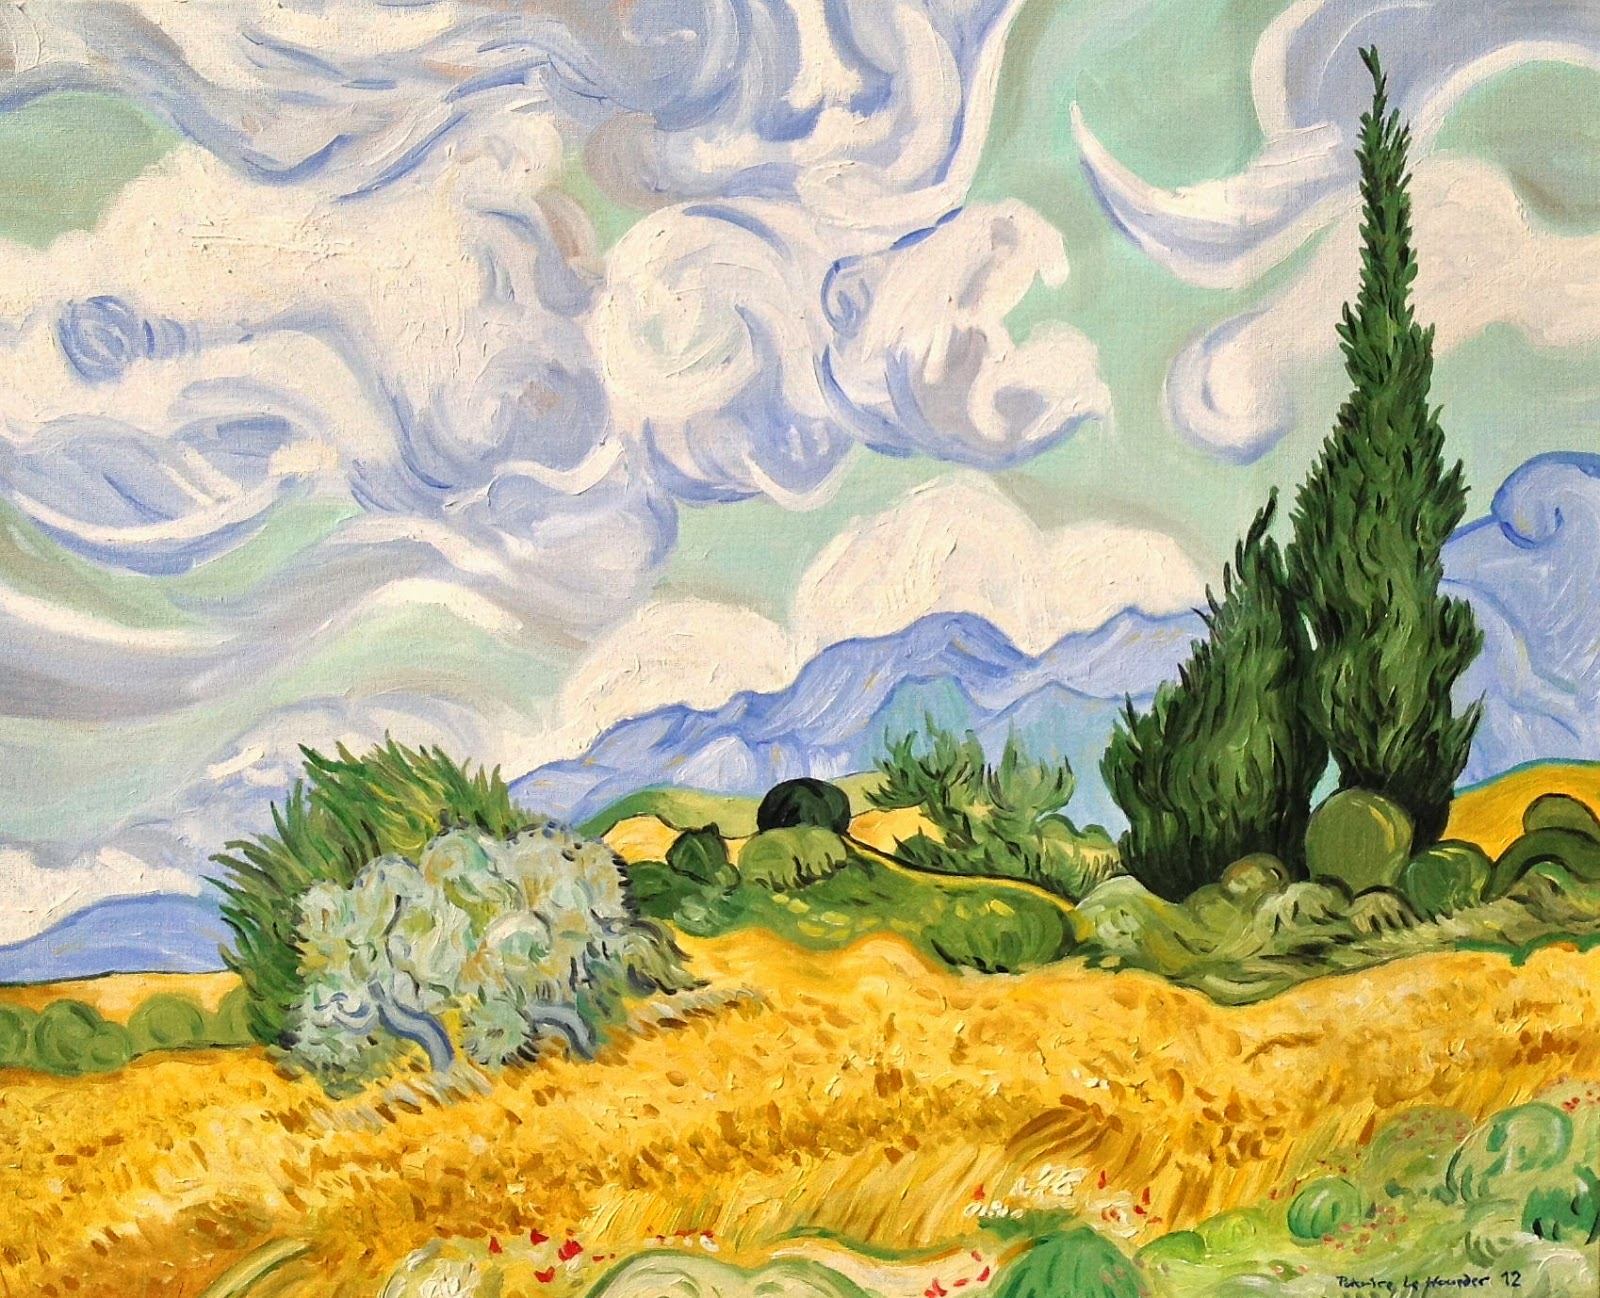
\includegraphics[scale=1.25]{v}}} % Image background
\centering
\vspace*{5cm}
\par\normalfont\fontsize{35}{35}\sffamily\selectfont
\textbf{PROGRAMMER L'INTERNET DES OBJETS }\\
{\LARGE }\par % Book title
\vspace*{1cm}
{\Huge Laurent TOUTAIN}\par % Author name
\endgroup

%----------------------------------------------------------------------------------------
%	COPYRIGHT PAGE
%----------------------------------------------------------------------------------------

\newpage
~\vfill
\thispagestyle{empty}

%\noindent Copyright \copyright\ 2014 Andrea Hidalgo\\ % Copyright notice

\noindent \textsc{IMT Atlantique}\\

\noindent Basé sur le MOOC PLIDO.\\ % License information

\noindent \textit{Publié le \today} % Printing/edition date

%----------------------------------------------------------------------------------------
%	TABLE OF CONTENTS
%----------------------------------------------------------------------------------------


\chapterimage{pano-5.jpg} % heading image

\pagestyle{empty} % No headers

\renewcommand\contentsname{Table des Matières}
\renewcommand{\bibname}{Bibliographie}
\tableofcontents% Print the table of contents itself

%\cleardoublepage % Forces the first chapter to start on an odd page so it's on the right

\pagestyle{fancy} % Print headers again

%----------------------------------------------------------------------------------------
%	CHAPTERS
%----------------------------------------------------------------------------------------
\chapter*{Acronymes}
\begin{multicols}{2}
\begin{acronym}
\acro{3GPP}{3rd Generation Partnership Project}
\acro{ABP}{Authentication By Personalisation}
\acro{ADSL}{Asymmetric Digital Subscriber Line}
\acro{AMQP}{Advanced Message Queuing Protocol}
\acro{AS}{Application Server}
\acro{ASCII}{American Standard Code for Information Interchange}
\acro{BLE}{Bluetooth Low Energy}
\acro{CBOR}{Concise Binaire Object Representation}
\acro{CoAP}{Constrained Application Protocol}
\acro{Cosem}{Companion Specification for Energy Management}
\acro{CRC}{Cyclic Redundancy Check}
\acro{CSV}{Comma Separated Values}
\acro{DLMS}{Device Language Message Specification}
\acro{DTT}{Digital Terrestrial Television}
\acro{DR}{Data Rate}
\acro{GSMA}{GSM Association}
\acro{HTML}{HyperText Markup Language}
\acro{HTTP}{HyperText Transport Protocol}
\acro{HTTPS}{HyperText Transport Protocol Secure}
\acro{IANA}{Internet Assigned Numbers Authority}
\acro{IBAN}{International Bank Account Number}
\acro{IEEE}{Institute of Electrical and Electronics Engineers}
\acro{IETF}{Internet Engineering Task Force}
\acro{IoT}{Internet of Things}
\acro{IP}{Internet Protocol}
\acro{IPv4}{Internet Protocol version 4}
\acro{IPv6}{Internet Protocol version 6}
\acro{IPSO}{IP for Smart Objects}
\acro{ITU}{International Telecommunication Union}
\acro{IRI}{International Resource Identifier}
\acro{ISBN}{International Standard Book Number}
\acro{ISO}{International Standardization Organization}
\acro{JMS}{Java Messaging Service}
\acro{JSON}{JavaScript Object Notation}
\acro{JSON-LD}{JavaScript Object Notation  for Linked Data}
\acro{LCIM}{Levels of Conceptual Interoperability Model}
\acro{LPWAN}{Low Power Wide Area Network}
\acro{LwM2M}{Lightweight Machine to Machine}
\acro{LNS}{LoRaWAN Network Server}
\acro{MQTT}{Message Queuing Telemetry Transport}
\acro{NAT}{Network Address Translation}
\acro{NGW}{Network GateWay}
\acro{NIDD}{Non IP Data Delivery}
\acro{OMA}{Open Mobile Alliance}
\acro{OTAA}{Over The Air Authentication}
\acro{OVH}{On Vous Herbèrge}
\acro{PAC}{Porting Authorization Code}
\acro{REST}{REpresentational State Transfer}
\acro{RFC}{Request For Comments}
\acro{RGW}{Radio GateWay}
\acro{RNIPP}{Répertoire National d'Identification des Personnes Physiques}
\acro{RSSI}{Received Signal Strength Indicator}
\acro{RTT}{Round Trip Time}
\acro{SCEF}{Service Capability Exposure Function}
\acro{SenML}{Sensor Measuring List}
\acro{SCHC}{Static Context Header Compression}
\acro{SF}{Spreading Factor}
\acro{SNR}{Signal to Noise Ratio}
\acro{SSID}{Service Set IDentifier}
\acro{STIC}{Sciences et Technologies de l’Information et de la Communication}
\acro{TCP}{Transmission Control Protocol}
\acro{TLV}{Type Length Value}
\acro{TNT}{Télévision Numérique Terrestre}
\acro{TTN}{The Things Network}
\acro{UDP}{User Datagram Protocol}
\acro{UIT}{Union internationale des télécommunications}
\acro{UNB}{Ultra Narrow-Band}
\acro{URI}{Universal Resource Identifier}
\acro{URL}{Univeral Resource Locator}
\acro{URN}{Univeral Resource Name}
\acro{VPS}{Virtual Private Server}
\acro{W3C}{World Wide Web Consortium}
\acro{WWW}{World Wide Web}
\acro{XML}{Extensible Markup Language}
\acro{XMPP}{Extensible Messaging Protocol et Presence}
\end{acronym}
\end{multicols}

\chapterimage{pano-tv1.png} % Chapter heading image
\cleardoublepage
\chapter{LES BASES DE L'INTERNET DES OBJETS (IOT)}

\section{Introduction}

  \vspace{1em}
 \begin{wrapfigure}{r}{3cm}
\Youtube{https://youtu.be/9edD2jEF3vM}
\end{wrapfigure}
 Dans cette première partie du cours, nous allons poser les bases de ce qu'est l'internet des objets (\ac{IoT} in english). Qu'est-ce qu'on entend par \ac{IoT} dans le cadre de livre~? Quelles sont les problématiques auxquelles doit répondre l'\ac{IoT} et son évolution aujourd'hui~? Quelles sont les technologies, les architectures, les protocoles sous-jacents qui seront utilisés dans cet ouvrage~? 
 
 Pour cela, nous allons faire un parallèle entre la manière dont l'internet a intégré la télévision et ce que l'on vit actuellement avec l'internet des objets. 
 
 \subsection{Réseaux dédiés}
   \vspace{1em}

\begin{wrapfigure}{r}{6cm}
\centerline{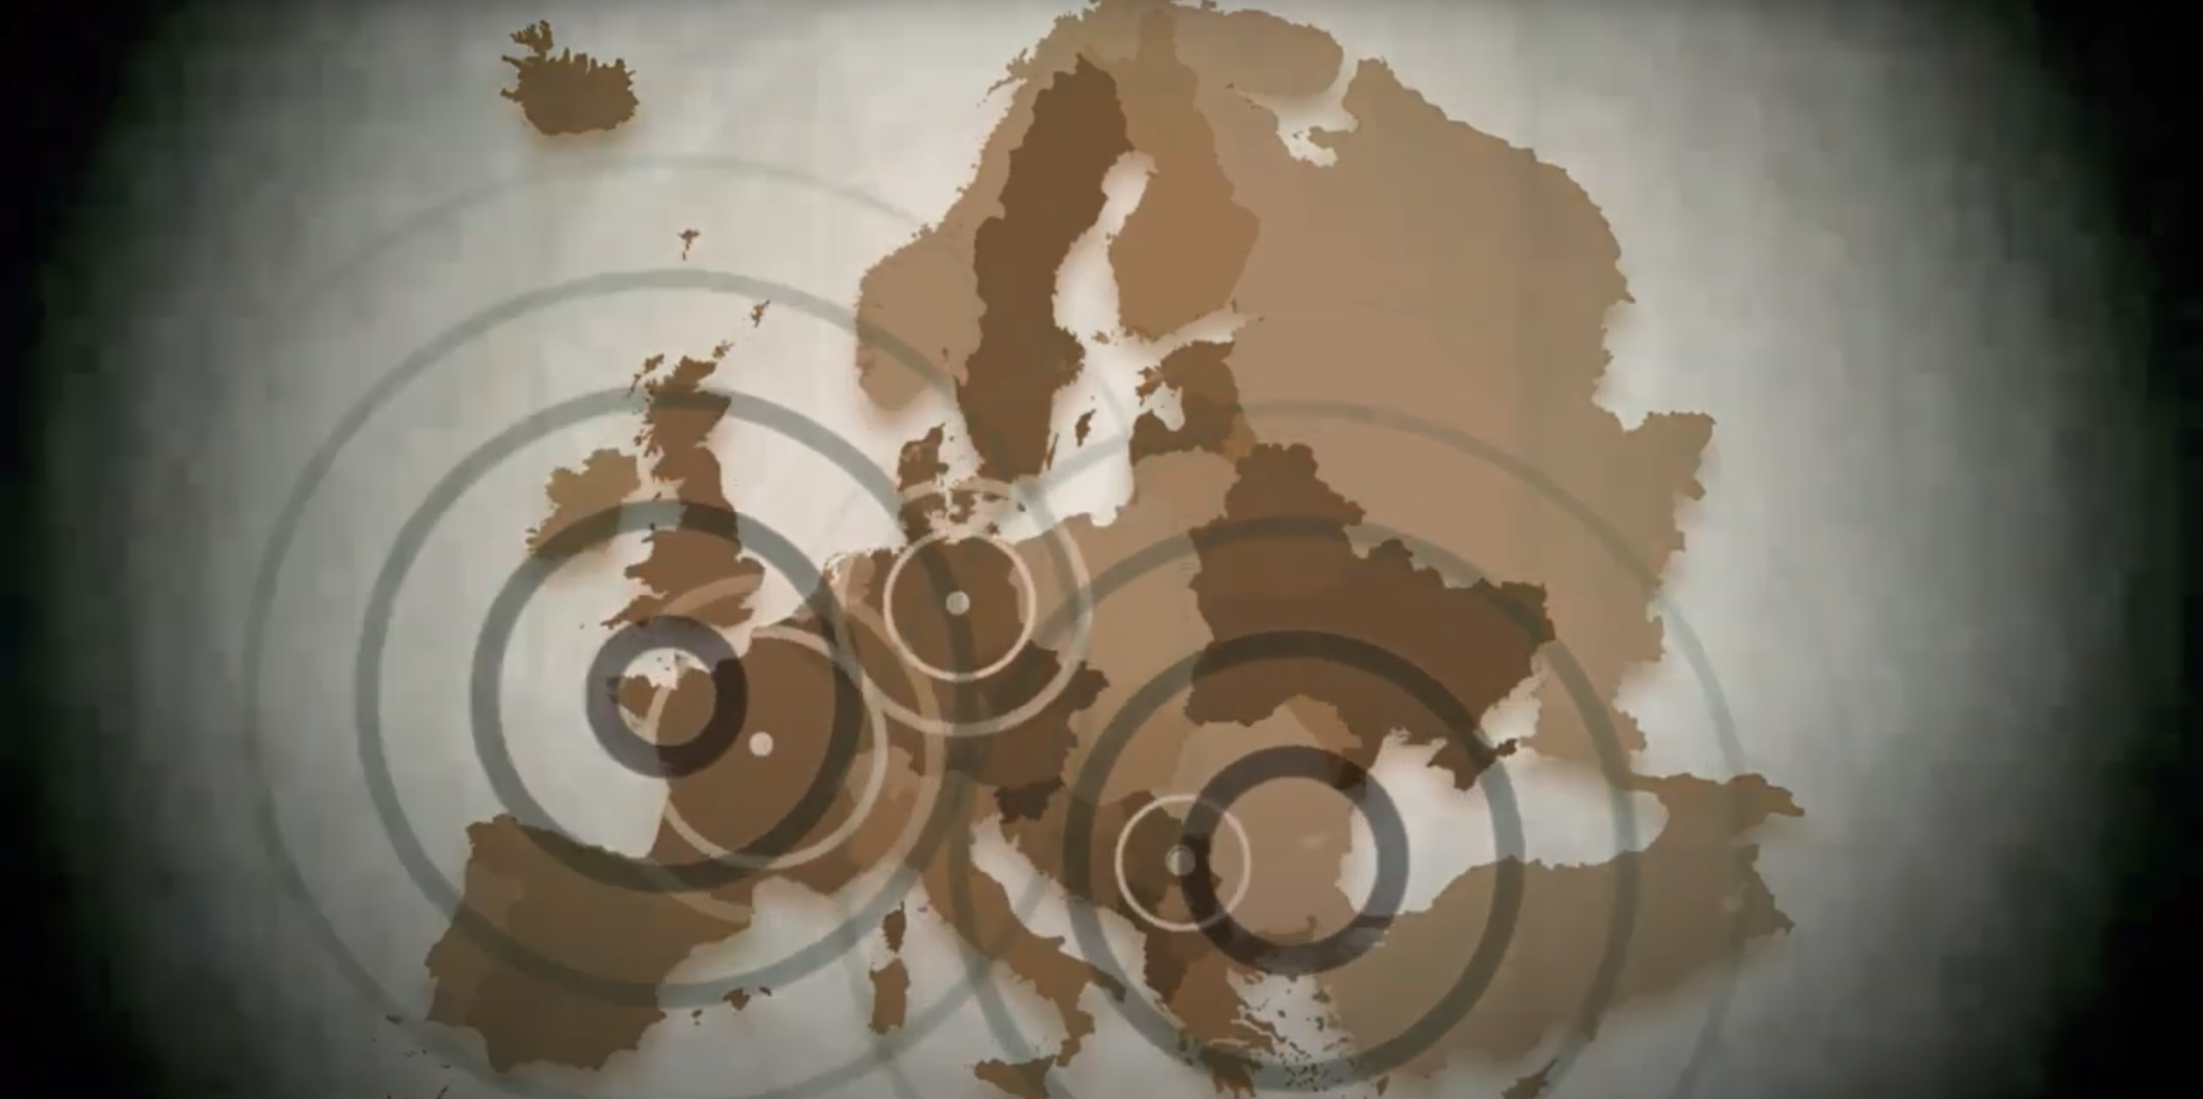
\includegraphics[width=.4\columnwidth]{Pictures/illu-propa.png}}
\end{wrapfigure}

 Dans les années 50, la télévision est devenue très populaire et presque tous les foyers ont acheté un téléviseur pour regarder leurs programmes préférés. Des réseaux de transmission dédiés ont été déployés partout sur la planète. En fait chaque type de communication avait son propre réseau un pour la radio un pour le téléphone un pour le télex,...
 


Dans les années 80, l'internet a vu le jour, mais les vitesses de transmission était faible et le réseau était limitée aux chargements de fichiers. Dans les années 90, des images et l'hypermédia avec le \ac{WWW} sont apparus, en lien avec l'augmentation des débits. Toujours dans les années 90, l'augmentation en puissance des microprocesseurs a permis la numérisation du signal télé. Les téléviseurs ont commencé à inclure des microprocesseurs et les réseaux sont passés d'une transmission analogique au numérique ; mais ils sont restés dédié à cet usage unique diffuser la télévision. Avec l'entrée dans le nouveau millénaire, l'internet a gagné en débit avec l'\ac{ADSL} et des fibres optiques. Il était possible d'intégrer des images dans les pages web mais la qualité était médiocre. Au même moment des centaines de canaux de télévision diffusaient en haute résolution leur programme via satellite ou par \ac{TNT}. De nos jours les communications internet ont gagné en vitesse et en qualité et certains pays ont coupé la \ac{TNT} et choisi de ne transmettre leurs programmes que par internet. En fait l'utilisation d'internet n'est pas uniquement un changement de réseau de distribution c'est aussi un changement majeur dans les usages et les applications. Vous pouvez regarder la télévision sur votre téléphone portable ou même regarder votre série favorite quand vous le voulez, à la demande. 

  \vspace{2em}

\subsection{3 phases technologiques}
   \vspace{1em}

\begin{wrapfigure}{r}{6cm}
\centerline{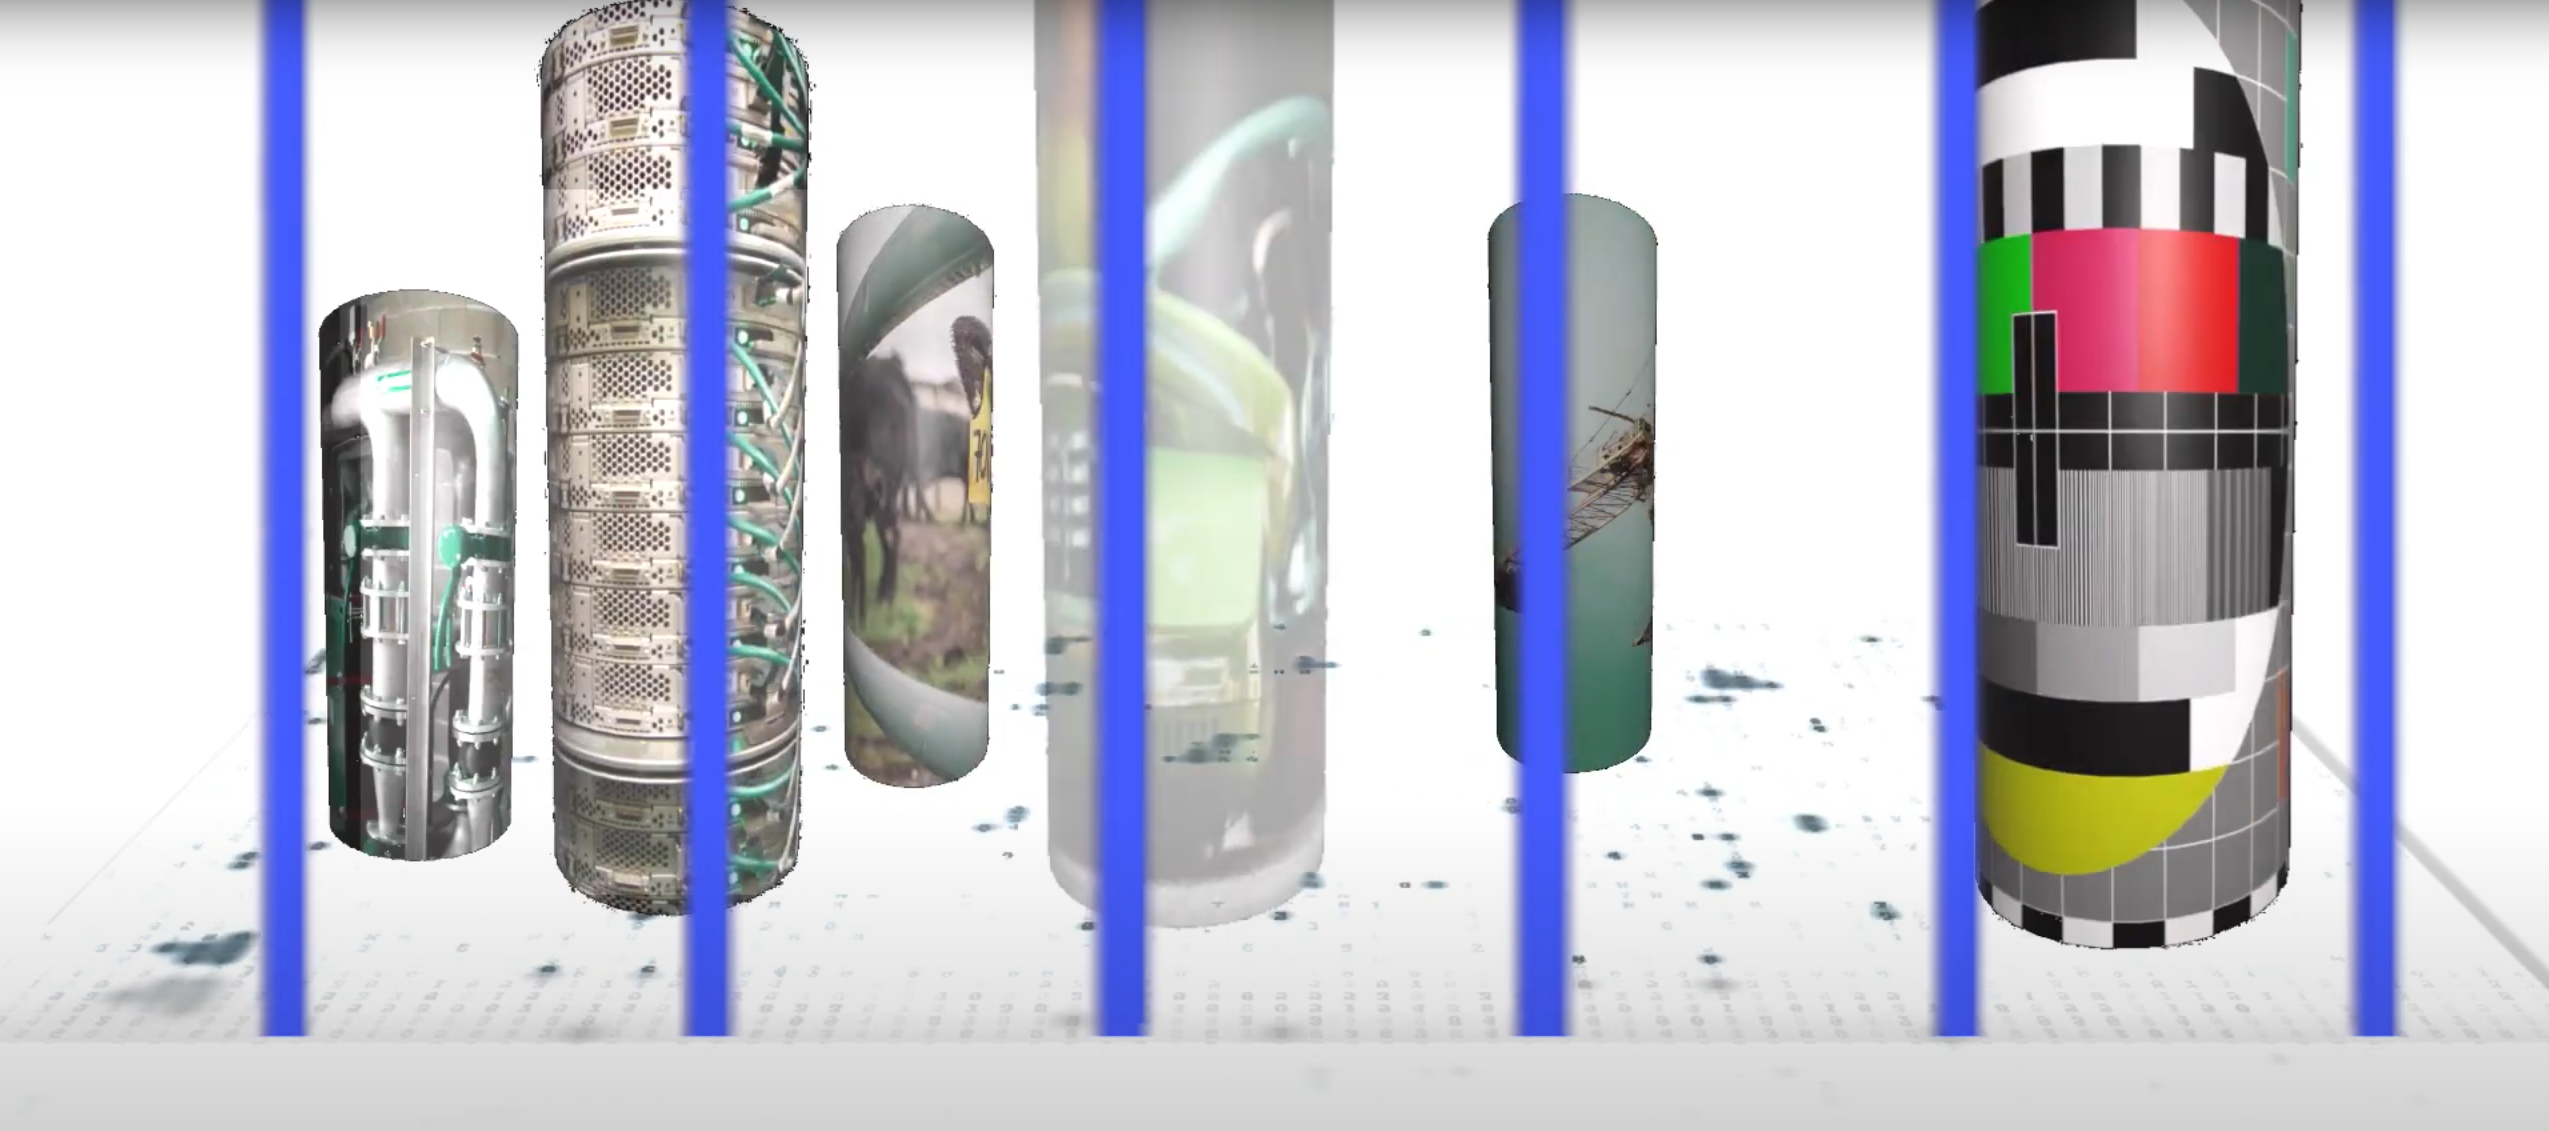
\includegraphics[width=.4\columnwidth]{Pictures/illu-verticals.png}}
\end{wrapfigure}
De cet exemple, on peut définir trois phases dans le développement d'une technologie. Dans la première phase, un réseau spécifique est construit pour un usage bien défini. On appelle cela une approche \Index{verticale} ; une technologie est dédiée à un seul usage. Il est difficile d'échanger de l'information entre deux verticales. On fait aussi référence à des \Index{silos} car ils sont isolés. Dans une seconde phase, les verticales commencent à intégrer des technologies communes mais pas d'une manière coordonnée. Elles ne peuvent toujours pas communiquer facilement car elles n'ont pas fait les mêmes choix.

~

\begin{wrapfigure}{r}{6cm}
\centerline{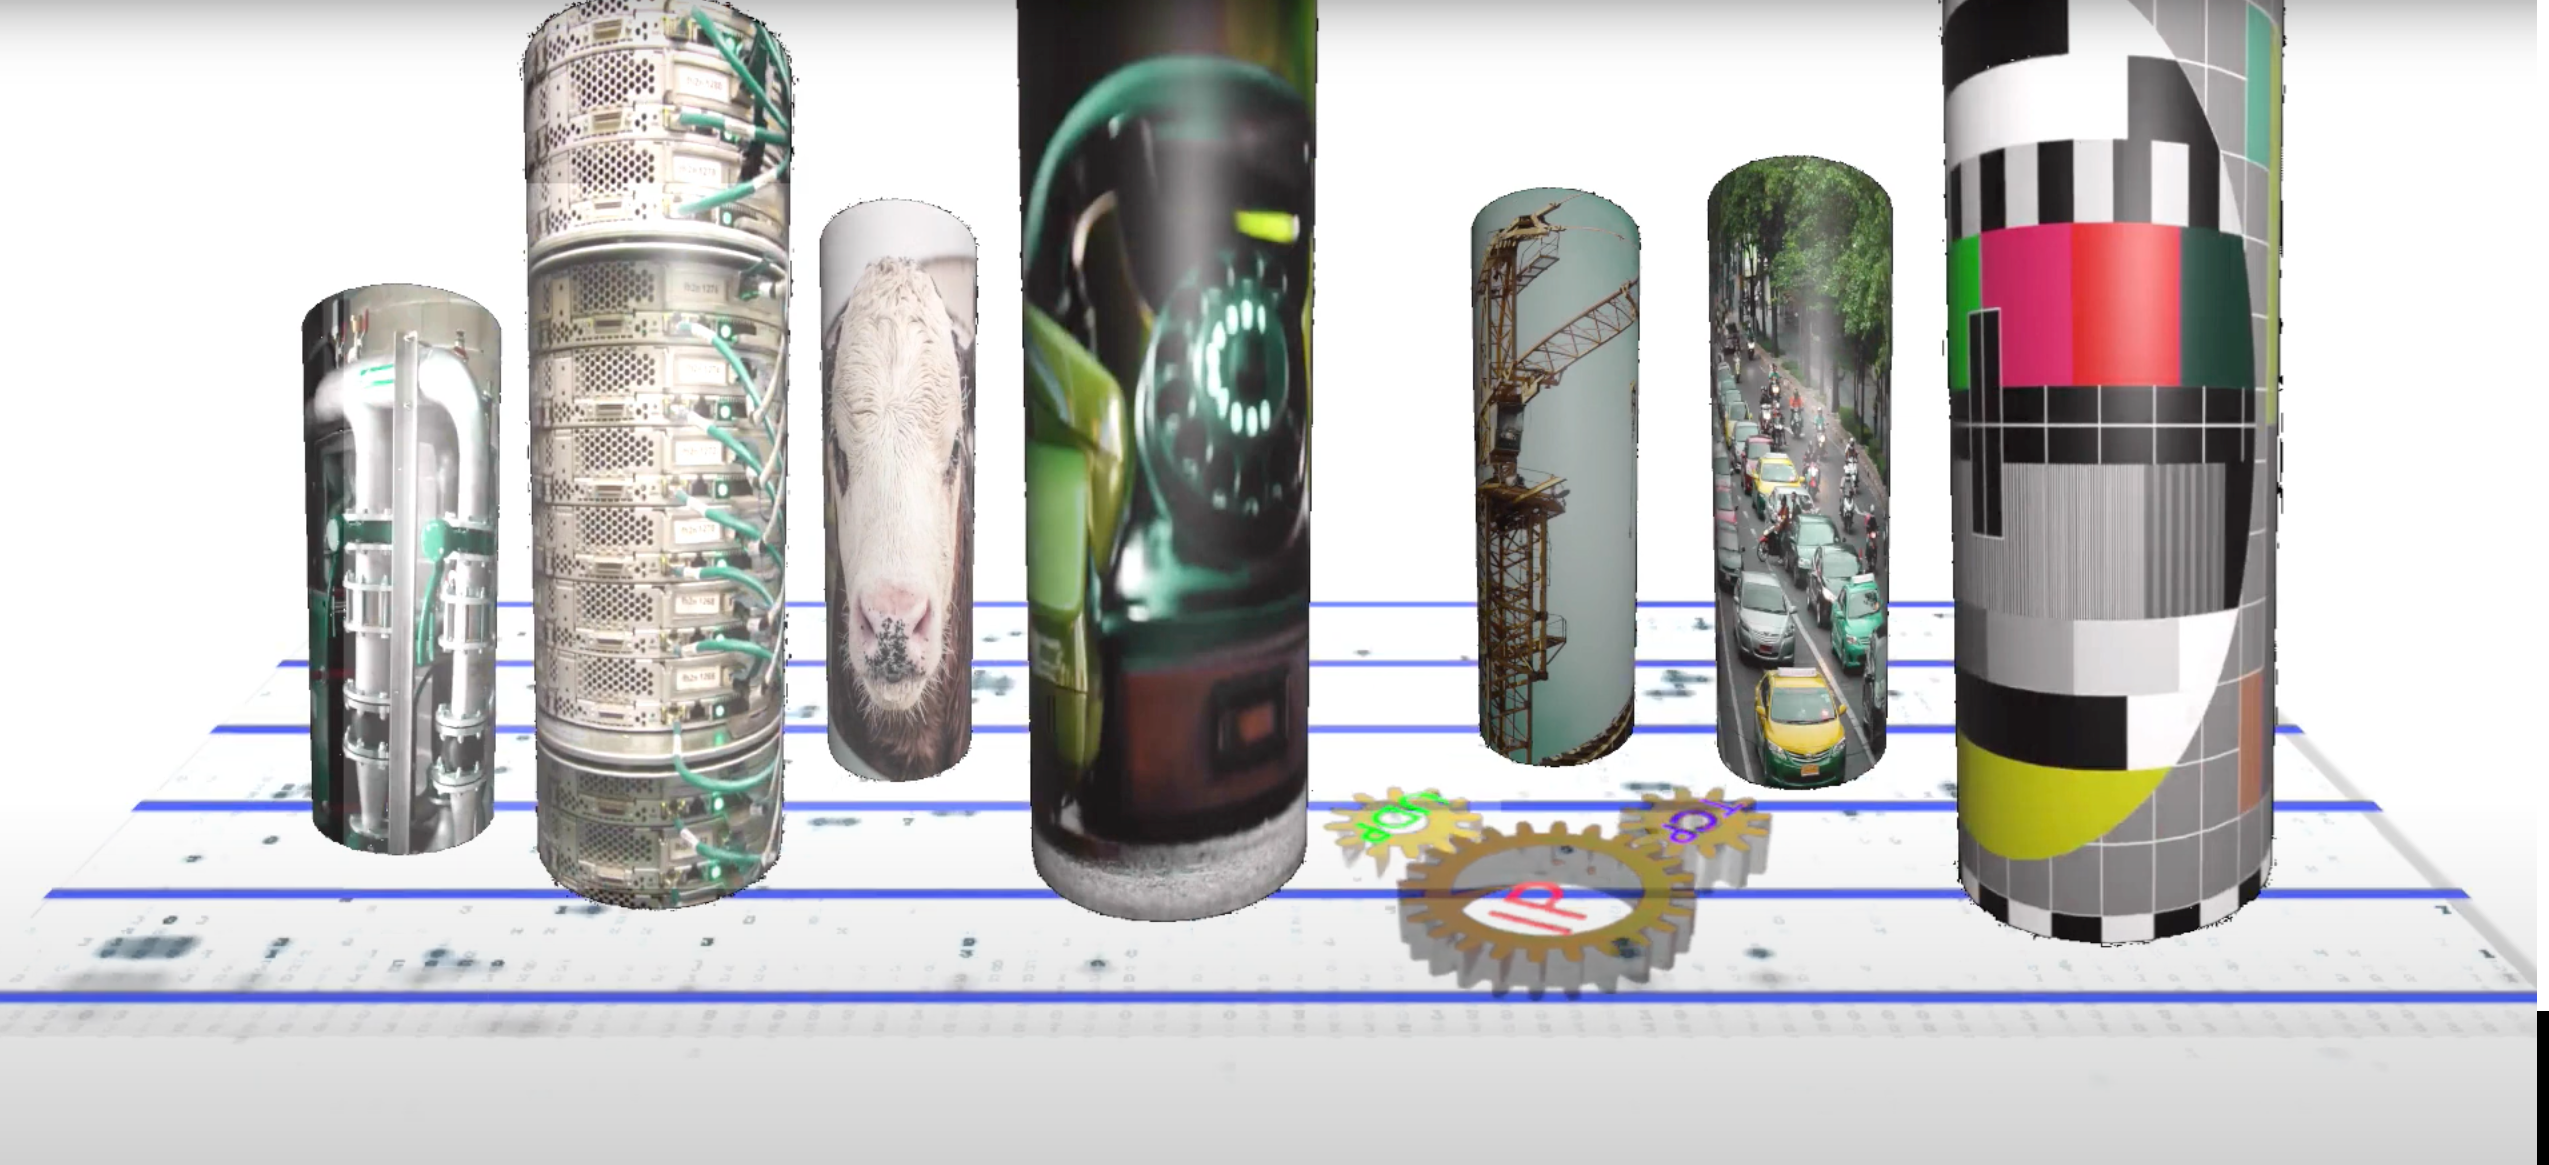
\includegraphics[width=.4\columnwidth]{Pictures/ill-horizontales.png}}
\end{wrapfigure}
Dans une dernière phase, des verticales se coordonnent pour converger vers les mêmes technologies en définissant des règles et des usages communs. Ceci dans le but de réduire les coûts ou d'augmenter leur impact dans ce cas. On parle d'horizontal\index{Horizontale} car elle couvre plusieurs secteurs. L'internet est devenu une de ces horizontales pour beaucoup de services. L'internet des objets suit ce même mouvement. Des solutions particulières ont émergé pour résoudre des besoins spécifiques en agriculture, dans l'automobile, dans la santé, dans l'énergie. Quand les réseaux internet ont permis des communications à faible coût, l'architecture de l'internet a été prise en compte mais sans compatibilité. Le changement qu'on vit actuellement est la définition de fonctionnalités communes à différents domaines. Le but étant de réduire les coûts mais également de croiser les informations pour une meilleure gestion du processus industriel et un meilleur usage des ressources
 

  \vspace{2em}

\section{L'Internet des Objets}

  \vspace{1em}
  
 Comment définir l’internet des objets~? Ou plutôt, quel internet des objets allons-nous étudier~? L’ambiguïté des deux termes "internet" et "objets" impose une définition plus précise ; ou du moins une classification pour mieux comprendre à quoi l’on fait référence.

  \vspace{1em}


L’internet est maintenant totalement intégré dans nos vies, pour le travail, l’enseignement, pour les distractions. On l’utilise à la maison ou au travail sur nos ordinateurs, et on l'emporte avec nous de plus en plus avec nos smartphones. 

Chacun a sa définition de ce qu’est internet. Pour le grand public, il peut s’agir d’applications très populaires comme Facebook, Tik-Tok, Netflix, Zoom. Pour certains, un peu plus technophiles, l’internet peut être confondu avec le Web auquel on accède via Chrome ou Firefox. Les techniciens parleront de protocoles comme IP, TCP, HTTP, et d’adresses comme les adresses IP ou les URL.

~~

Comme ce livre est orienté technologie, notre approche relève plutôt de cette dernière catégorie. Nous verrons comment des protocoles développés il y a une vingtaine d’années pour des ordinateurs peuvent s’appliquer à d’autres dispositifs qu’il nous reste à définir.

L'objectif de l'internet des objets est de poursuivre l'intégration du réseau Internet pour permettre à autre chose que des ordinateurs d'échanger des données. Le but principal est d'optimiser les processus pour qu'ils soient plus efficaces pour économiser des ressources ou d'augmenter la productivité. Il s'agit donc d'un internet enfoui, loin du frigo ou de la montre connectés, qui vont remonter des informations avec une infrastructure ou d'autres équipements. On peut imaginer des capteurs dans une usine pour contrôler la production, des voitures connectées qui vont dialoguer pour éviter les collisions, la mesure du taux de remplissage des bennes de recyclage dans une ville pour optimiser les circuits de collecte, la surveillance du degré d'humidité d'un champ pour réduire la consommation d'eau...


L’internet des objets peut se résumer de la manière suivante : utiliser des protocoles développés pour des ordinateurs et maintenant des téléphones portables (plus puissants que les ordinateurs utilisés par l’internet à ses débuts) mais dans des environnements plus contraints. En effet, les lois de Moore, définissant les puissances de traitement des processeurs ainsi que la diminution continue des coûts de la mémoire, nous ont permis de doter les petits objets de ressources comparables à celles des ordinateurs d’il y a trente ans.

L’internet des objets, c’est résoudre l’équation suivante : continuer à faire la même chose car tous les systèmes d’information actuels utilisent les mêmes principes mais le faire différemment car ces principes sont trop coûteux en énergie, en temps de calcul et échange de données.

L’\ac{IoT}, l’internet des objets ou des choses, est une architecture globale permettant à des objets (équipements de même type ou non), d’interagir de manière autonome via internet. Cette interaction :

\begin{itemize}
    \item est réalisée, par construction, au travers d’un réseau internet, ce qui implique généralement que les objets/choses soient pourvus d’une adresse IP ;
    \item est relatif à des commandes (opérations de contrôles ou appels de fonctions) ou des échanges de données ou d’informations.
\end{itemize}

  \vspace{1em}


Ce nouveau paradigme \ac{STIC} qu’est l’IoT est une convergence de nombreux domaines d’applications tels que : les maisons ou bâtiments intelligents, les villes du futur, l’industrie du futur (industrie 4.0), l’énergie, les systèmes de transport, l’agriculture, la eSanté, etc., vers une suite protocolaire réduite, interopérable et sécurisée. Le mouvement est en marche et, vu le nombre d'acteurs concernés, va prendre plusieurs années. Mais les bases sont déjà bien établies et c'est ce que vous allez apprendre dans cet ouvrage.

 \vspace{2em}
 
\section{Le problème}

  \vspace{1em}

Un des problèmes que rencontre l’internet des objets, c’est que l’IoT ne démarre pas ex-nihilo. Maintenant que les technologies qui ont fait le succès de l'Internet sont matures, il ne s'agit pas juste de les appliquer à un nouveau domaine. Des objets étaient capables de communiquer bien avant qu’internet n’existe. Chaque secteur a déjà développé ses solutions, plus ou moins standards, plus ou moins propriétaires.

La figure~\vref{fig-bazar} reprend un certain nombre de travaux et de groupes qui spécifient les protocoles pour l’internet des objets. 

\begin{figure}[tbp]
\centerline{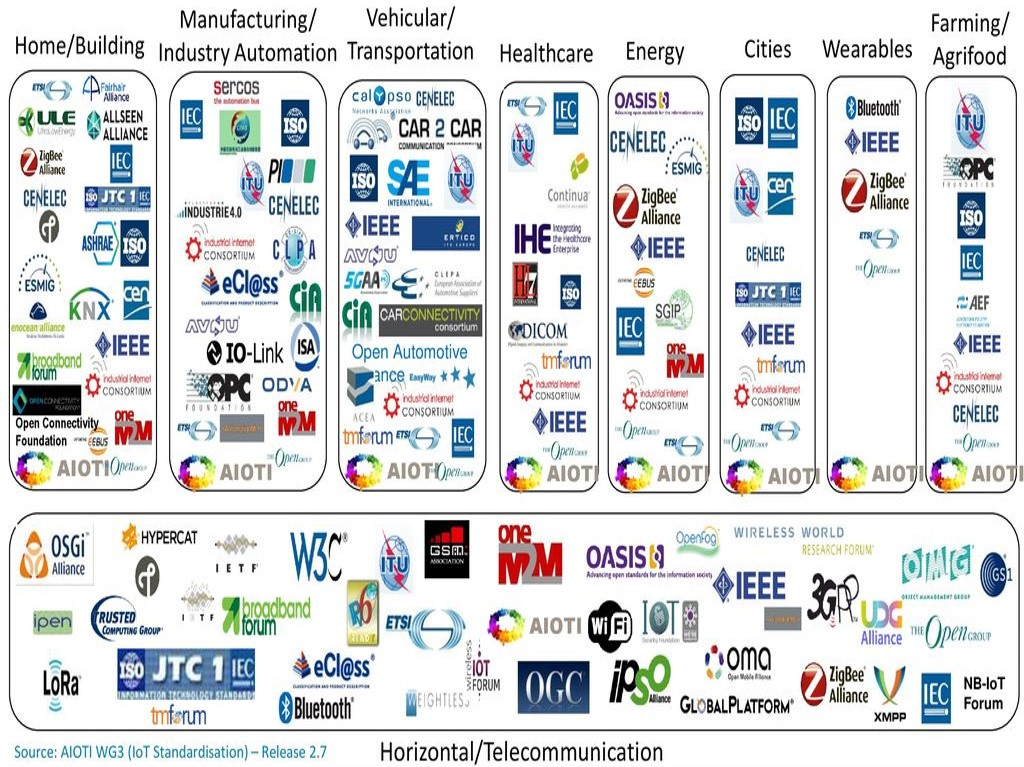
\includegraphics[width=1\columnwidth]{Pictures/IOTBazar_Domaines.jpeg}}
\caption{Quelques standards de l'IoT}
\label{fig-bazar}
\end{figure}

Sans entrer dans les détails, on voit que certains logos se retrouvent à plusieurs emplacements, qu’il y a pour chaque secteur une profusion de solutions qui nuisent à l’interopérabilité et aux évolutions. L’internet des objets, dans son acception la plus large, consiste à simplifier cette architecture, comme l’internet l'a fait il y a quelques années dans le domaine des télécoms en simplifiant ce modèle et en permettant à ces différents acteurs de converger vers une architecture commune et un ensemble de solutions plus réduit.

Cela ne veut pas nécessairement dire moins d’acteurs, mais une plus grande cohérence dans les choix technologiques.

La figure~\vref{fig-bazar-OS} analyse l’IoT par domaine d’application en se focalisant sur la composante réseau. L’IoT et les objets connectés sont des systèmes complexes pour lesquels les solutions open source, les alliances entre industriels, les organismes de standardisation sont toujours fragmentés ; cependant de manière moins importante, montrant que la structuration est en marche.

\begin{figure}[tbp]
\centerline{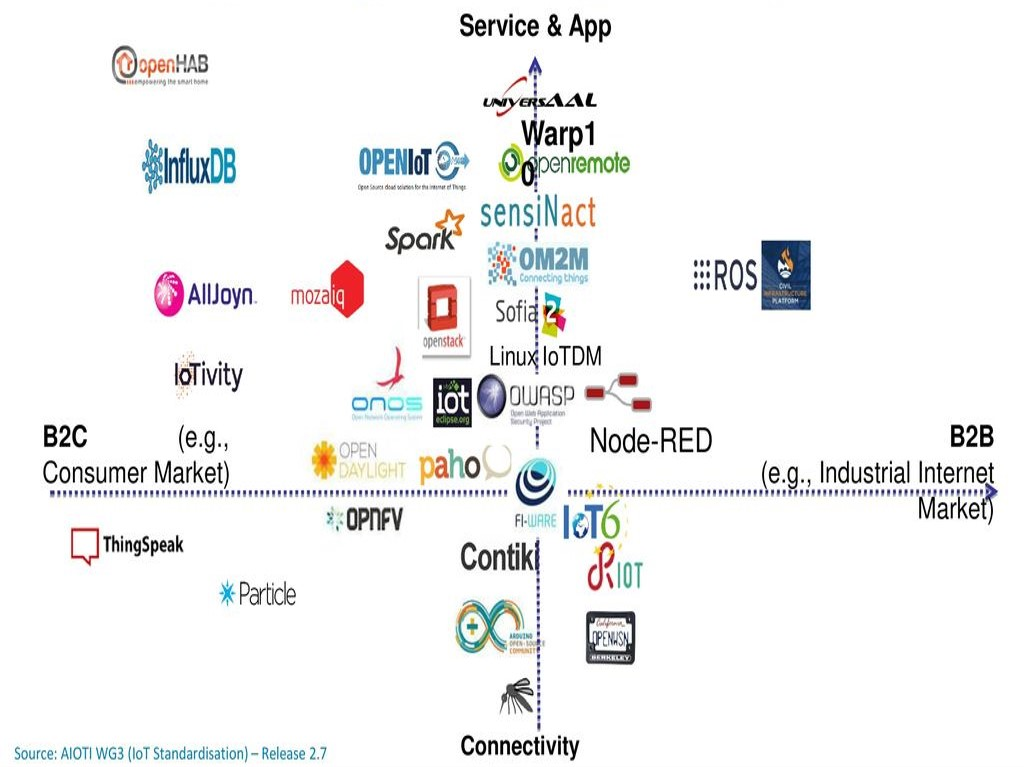
\includegraphics[width=1\columnwidth]{Pictures/IOTBazar_OpenSources.jpeg}}
\caption{Quelques applications Open Source pour l'IoT}
\label{fig-bazar-OS}
\end{figure}

Cette fragmentation de l’écosystème est paradoxale. Si l’on résume sommairement, les solutions proposées reviennent à interroger un équipement sur le terrain pour accéder à une valeur, la traiter et renvoyer une commande pour interagir avec l’environnement.

Pourquoi cette foison de solutions différentes~? Cela peut venir des besoins de fiabilité, de sécurité, de portée de la donnée, mais cela vient aussi de l’histoire. La communication avec des objets est tout aussi ancienne que la communication entre ordinateurs (qui sont eux-mêmes des objets). Mais à l’époque, chaque domaine a suivi sa propre voie en spécialisant les solutions pour répondre à ses besoins propres. Il en résulte des solutions optimisées pour un domaine particulier. Mais chaque fois qu’il faut modifier une technologie, le travail doit être adapté pour chaque domaine, introduisant des coûts et des délais supplémentaires.

De même, chaque domaine ayant sa propre représentation des données, il est relativement difficile de les combiner pour avoir une vision plus globale. On arrive donc à des systèmes fermés, chers, peu évolutifs, mais optimisés pour les tâches qu’ils ont à réaliser.

Au fil du temps, les protocoles de l’internet ont pu être utilisés, mais il s’agit surtout de complémenter les technologies existantes sans qu’il soit possible d’interconnecter deux domaines.


  \vspace{2em}

\section{Evolution de l'IoT}

  \vspace{1em}

L’exemple de l’évolution du réseau de télévision est éloquent. À ses débuts, ce réseau est analogique et hautement spécialisé pour diffuser les programmes transportés sur des signaux analogiques sur des équipements spécialisés, les téléviseurs.

Avec les progrès des processeurs informatiques, il devient possible de transporter les données en utilisant un codage numérique. Mais des réseaux spécialisés restent nécessaires, l’Internet n’offrant pas la même qualité.



La dernière étape consiste à intégrer ces flux dans l’internet classique. Cela devient possible par la montée en débit des réseaux filaires et radio (Wi-Fi, 4G...). 

Cette mutualisation des accès via l’internet permet non seulement une réduction des coûts, mais aussi l'apparition de nouveaux usages comme la télévision sur les téléphones portables ou les séries à la demande.

L’internet des objets suit la même voie. En plus des technologies spécifiques, les protocoles de l’internet sont intégrés, mais en les adaptant aux contextes du secteur.  Nous sommes actuellement en train de vivre la convergence vers un ensemble réduit de protocoles, une standardisation de la représentation de la donnée, et son traitement sur des plates-formes plus génériques. 

Le déclencheur n’est pas la montée en débit comme pour la télévision, mais la possibilité d'avoir des équipements peu chers, aux capacités réduites par rapport à l'informatique traditionnelle et autonomes énergétiquement, tout en ayant une meilleure intégration dans les systèmes d'information actuels.  

  \vspace{2em}

\section{Des objets contraints}

  \vspace{1em}

Avec les progrès de l’électronique, les processeurs deviennent de plus en plus puissants et les super-ordinateurs d’hier sont maintenant dans une montre ou un smart-phone. 

Pour l’internet des objets, la logique est un peu différente. La loi de Moore va induire une réduction des coûts de fabrication plutôt qu'une augmentation des puissances de traitement. Le principal critère pour un internet des objets massif reste l’énergie ; connecter un appareil à une source d’énergie ou recharger une batterie a un coût. Augmenter la vitesse du processeur ou la taille de la mémoire induit une plus grande consommation d’énergie de l'objet. On peut donc s’attendre à une certaine stabilité des performances des objets car ceux-ci resteront limités en performances.

Les objets sont généralement limités en termes de puissance de traitement, de mémoire et d’énergie. Selon le standard de l’IETF \rfc{7228}, les dispositifs peuvent être répartis en trois classes qui se retrouvent aussi dans la segmentation des processeurs :

\begin{itemize}
\item La classe 0, avec moins de 10 ko de mémoire volatile pour stocker les données temporaires et 100 ko de mémoire Flash pour stocker le code informatique de l'objet. C'est l’équivalent d’un Arduino UNO (2 ko de RAM et 32 ko de Flash). Il est presque impossible d’installer à la fois les protocoles utilisés pour communiquer sur Internet (même de manière restreinte) et les applications qui tournent dessus. 
\item La classe 1 a environ 10 Ko de RAM et 100 Ko de Flash. Avec une adaptation, il est possible d’y installer une pile IP. Il s'agit par exemple d'équipement comme le Pycom Lopy4 que nous utiliserons par la suite (et qui se situe dans la limite haute) sur lequel le système d'exploitation est minimal. Ainsi, le Pycom utilise une version simplifiée du langage Python (micro-python) qui permet de l'adapter à la limitation du système.
\item La classe 2 est moins restreinte avec au moins 50 ko de RAM et 250 ko de Flash (comme un Raspberry Pi). Le système d’exploitation Linux peut fonctionner sur ces appareils. Par conséquent, il y a peu de limitations sur la pile IP et les applications s’y exécutant.
Les appareils de classe 1 ont trop de restrictions pour utiliser les protocoles définis pour des objets plus gros. L’\ac{IETF}, l'organisme qui standardise les protocoles de l'internet, a proposé une révision de sa pile de protocoles afin d’adapter sa pile protocolaire à un environnement contraint.
\end{itemize}


La figure~\vref{fig-encap} résume les moyens d'interconnexion suivant la classe de l'objet~:
Un appareil de classe 0 ne peut pas utiliser directement l’internet pour échanger des informations, d’où la nécessité d’installer une passerelle pour capter le trafic et l’envoyer sur l’internet. Il ne possède pas directement d'adresse IP. Les passerelles LoRaWAN \ac{LNS} et \acs{3GPP} \ac{SCEF} agissent dans ce sens (nous reviendrons là-dessus). Les données produites sont encapsulées par ces passerelles dans des protocoles comme \ac{HTTP} ou \ac{MQTT}, que nous verrons également dans la suite du cours.

Les appareils de classe 1 peuvent aussi utiliser une passerelle pour s’interconnecter à l’internet traditionnel, mais plutôt que d'encapsuler les données produites dans d'autres protocoles comme le fait la classe 0, les passerelles pour les appareils de classe 1 vont traduire un protocole contraint dans son équivalent dans le monde non contraint.

Les dispositifs de classe 2 peuvent interagir directement avec d’autres nœuds sur l’internet, sans passer par une passerelle.

\begin{figure}[tbp]
\centerline{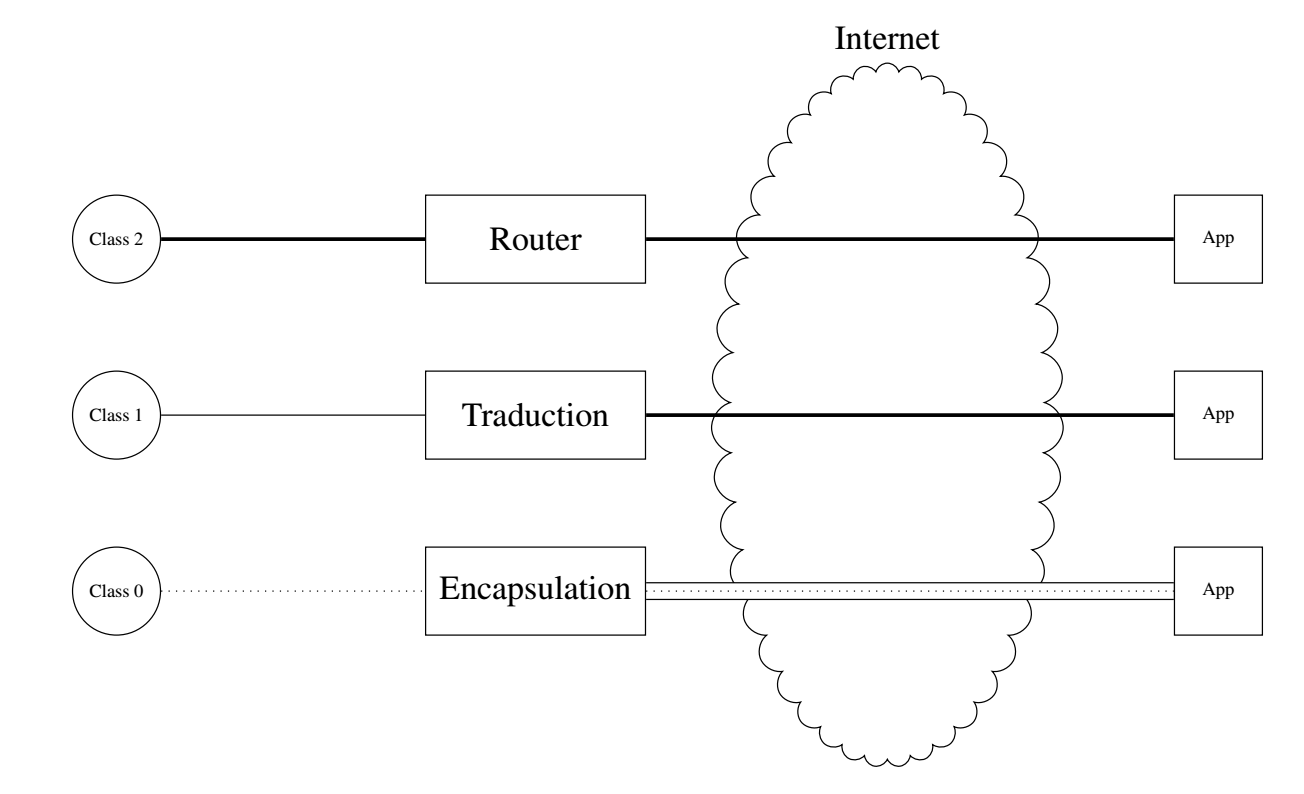
\includegraphics[width=1\columnwidth]{Pictures/Encpasul.png}}
\caption{Possibilités d'interconnection}
\label{fig-encap}
\end{figure}

  \vspace{2em}

\section{L'interopérabilité}

  \vspace{1em}


Un autre défi concerne le nombre de dispositifs. Certaines études prévoient 500 milliards de dispositifs à la fin de la décennie.

  \vspace{1em}
 \begin{wrapfigure}{r}{3cm}
\Youtube{https://youtu.be/2TQiTskfZtc}
\end{wrapfigure}
Avec cet énorme internet des objets, où presque chaque équipement comprendra des éléments de détection ou d’action, l’intégration dans un système d’information deviendra un véritable défi. Comme l’internet des objets actuel est conçu pour une verticale (c'est-à-dire pour des applications spécifiques), les dispositifs sont choisis et intégrés au moment de la conception du système. Les ingénieurs choisissent leurs capteurs, connaissent précisément leurs caractéristiques et écrivent leur code en fonction de ce qu'ils ont intégré. 

L’internet des objets massif change la donne. Les dispositifs ou les choses ne peuvent pas être intégrés dès le départ dans un système d’information statique. L’intégration doit se faire au fil du temps et doit gérer les évolutions des dispositifs pendant longtemps (les fabricants de dispositifs peuvent changer, les produits évolueront avec de nouvelles fonctionnalités, etc.)

Cette question d’interopérabilité a été formalisée dans le modèle \ac{LCIM}~\cite{tolk2003levels} (voir figure~\vref{fig-lcim}) peut être représenté par un compteur pour mesurer le degré d'interopérabilité.

\begin{figure}[tbp]
\centerline{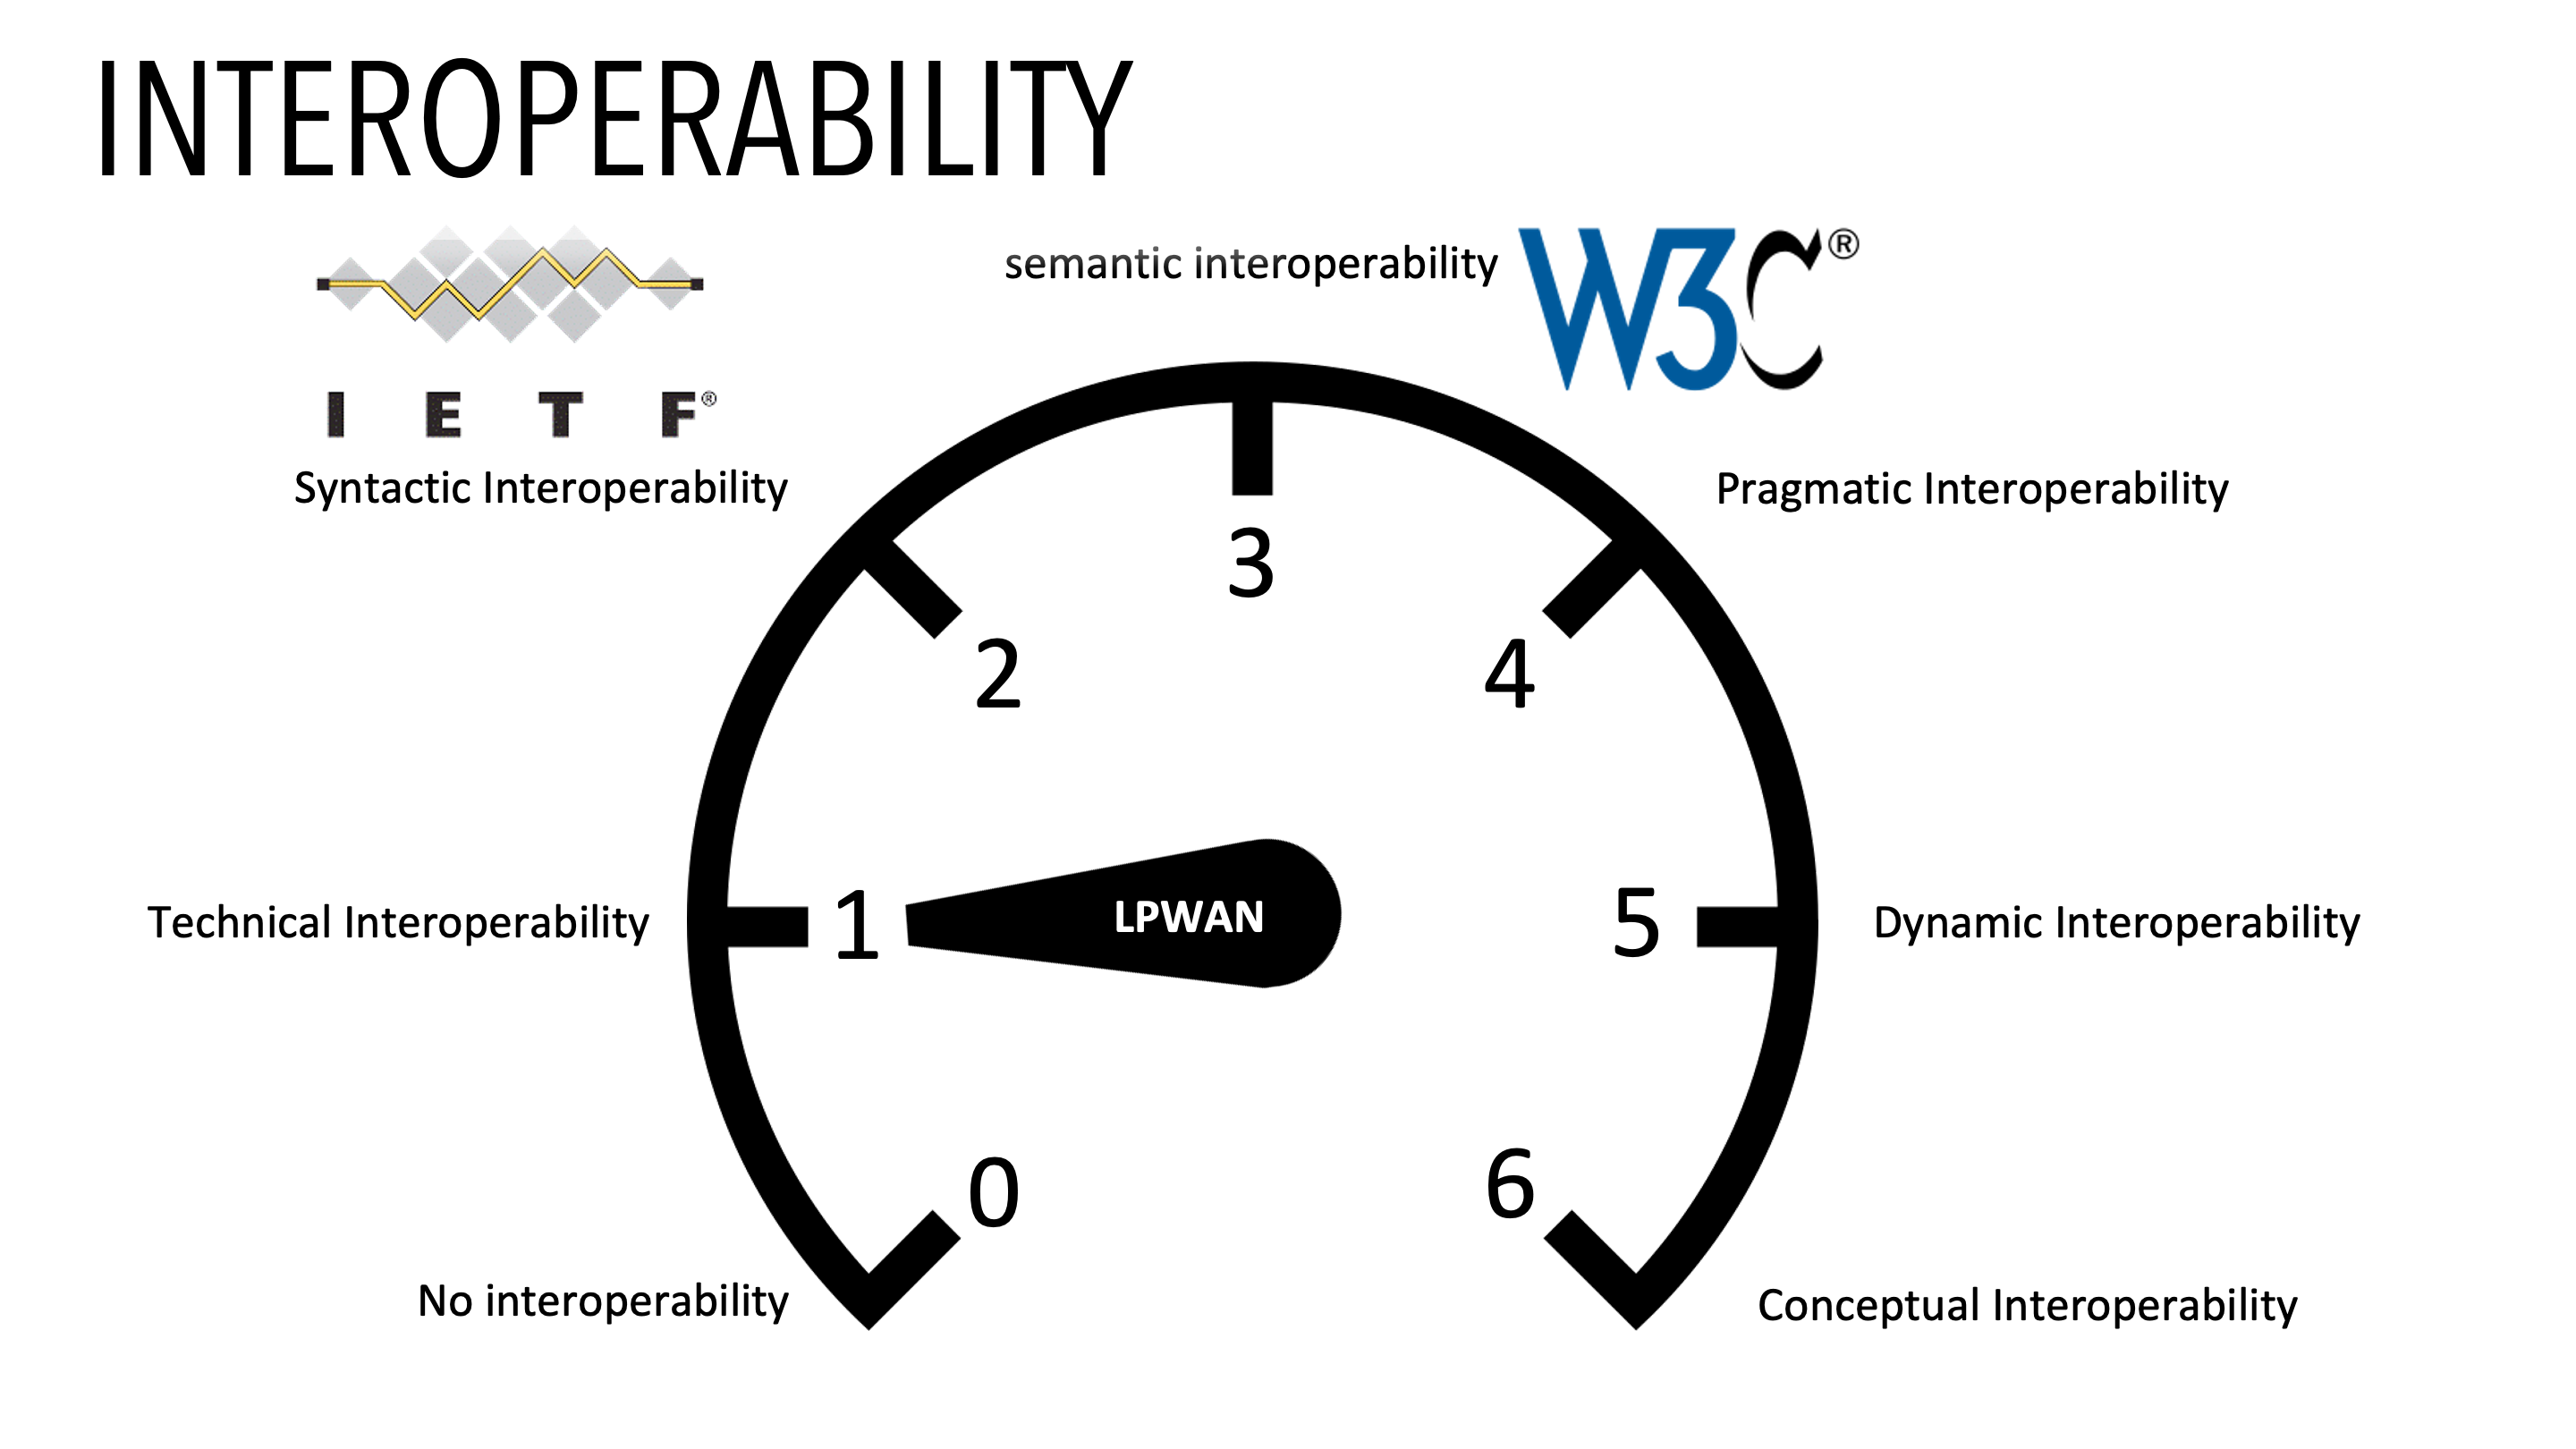
\includegraphics[width=1\columnwidth]{Pictures/TPT2020.png}}
\caption{Niveau d'interopérabilité}
\label{fig-lcim}
\end{figure}


Il distingue six niveaux d’interopérabilité, parmi lesquels :

\begin{itemize}
     \item Au niveau zéro, on n'est pas connecté ; on ne parle à personne donc on n'a pas de problèmes d'interopérabilité. 
    \item  Au niveau 1, on est capable de transmettre de l'information,  mais il faut que les deux côtés connaissent les règles. On a un système intégré ; les applications doivent  connaître précisément les spécifications des objets avec lesquels ils communiquent,  car elles définissent ses propres formats des échanges de données. On pourrait prendre l'exemple qu'une carte électrique où un processeur communique avec des capteurs via un circuit imprimé. Le code tournant sur le processeur peut être écrit à l'avance car il y a peu de chance qu'un utilisateur dessoude les composants pour les remplacer par d'autres. Cela correspond à l'encapsulation, si l'on considère les objets en réseau de la figure~\vref{fig-encap}, l'élément d'interconnexion doit être configuré pour en fonction de l'objet émetteur encapsuler les données vers la bonne application chez le bon récepteur. 
    \item L’interopérabilité syntaxique (niveau 2) où deux nœuds peuvent échanger des données, sans être a préalable configurés pour cet échange. C'est le cas de l'Internet. En utilisant cette suite de protocoles, en ayant une adresse valide sur le réseau, toute application est capable d'échanger des données avec une autre. En revanche, les données que vous allez échanger sont propres à une application. Les vidéoconférences sont un très bon exemple d'interopérabilité de niveau 2. Vous ne pouvez pas utiliser Zoom si votre correspondant utilise Teams car les formats sont différents. L'\ac{IETF}  est le regroupement de différents acteurs (industriels, académiques,...) qui produisent les standards liés à ce réseau. Il se reconnaissent par l'acronyme \ac{RFC} suivi d'un nombre. 
    \item L’interopérabilité sémantique (niveau 3) implique que le récepteur est capable d'interpréter les données reçues.Le web est un très bon exemple d'interopérabilité de niveau 3. Quel que soit votre navigateur, vous pouvez afficher les pages d'un site web et suivre les liens. Le sens de l'information est compris de la même manière des deux côtés. Pour le Web, le format \ac{HTML} permet à l'aide de balises (mots-clés) de structurer un texte en y ajoutant des informations de formatage ou des liens vers d'autres documents. Le W3C définit les standards.
     \item Les niveaux supérieurs d'interopérabilité vont être lié à la précision du modèle qui va représenter le système.     
\end{itemize}


L'internet qu'on connaît est une très bonne illustration du besoin d'interopérabilite. Il a permis, grace à une uniformisation du réseau et une force baisse des coûts de transmission, de développer de nouveaux usages. Vous n'auriez jamais investi pour un réseau propre à la vidéoconférence et au télétravail. Mais en mutualisant les usages, c'est possible ! L'internet des objets doit suivre la même voie et également converger vers l'architecture de l'internet actuel. Le mot clé est donc l'interopérabilité.  
   \vspace{2em}

\section{Le besoin de standardisation}
  \vspace{1em}

Les objets n'ont pas attendu l'internet pour communiquer. Ils ont évolué chacun dans leur verticale, développant des solutions satisfaisantes mais limitées en termes d'évolution et d'interopérabilité. Cet état des lieux sur la dispersion des écosystèmes met en avant la nécessité :

\begin{itemize}
\item d’une coordination entre les alliances ;
\item d’une harmonisation ou d’un alignement des standards ;
\item de disposer au plus vite d’implémentations de référence et de modèles de référence.
\end{itemize}

Dans le cas contraire, l’interopérabilité ne pourra pas être traitée comme il se doit, les nouveaux services innovants multi-domaines ne seront pas couverts, et le développement de l’IoT pourrait être freiné voire avorté.

Les aspects liés à l’éducation et à la formation des acteurs de l’IoT, ainsi que ceux liés à l’acceptation, aux usages et évidemment au volet socio-économique de l’IoT, sont aussi des points essentiels dont il faut tenir compte.

Les organismes de normalisation tels que l’\ac{IETF} ou le \ac{W3C} ont conçu des protocoles ou des modèles de données capables de traiter l’interopérabilité. D’une certaine manière, c’est la clé du succès de l’internet actuel. Il a permis de résoudre le problème de l’interopérabilité au niveau syntaxique et sémantique mais au prix de messages volumineux.

Le défi pour l’internet des objets est de s’intégrer dans ce système distribué géant. Comme l’internet des objets est un nouveau venu, l’évolution devra se faire de son côté pour prendre en compte les règles existantes, mais en les adaptant. Les prochains chapitres traiteront de ces changements.

\section{Questions}

\Question{Nouveau Domaine}{Les objets communicants sont un tout nouveau domaine, lié aux progrès en miniaturisation des composants électroniques:
\begin{itemize}[label=$\circ$]
\item \Wrong{Vrai}
\item \Correct{Faux}
\end{itemize}
 }{Les objets communicants ont toujours existé, même avant le déploiement des protocoles de l'Internet. Ce qui est nouveau c'est leur intégration dans les architectures Internet actuelle pour mieux traiter l'information qu'ils produisent.
 }
 
 \Question{Protocoles}{Laquelle de ces affirmations est vraie ?
\begin{itemize}[label=$\circ$]
\item \Wrong{Il y a très peu de protocoles pour faire communiquer les Objets. Comme l'Internet est une technologie qui s'est très répondue, son succès va permettre aux objets de communiquer.}
\item \Correct{ Il y a beaucoup de solutions pour permettre à des objets de communiquer, l'Internet des Objets doit permettre de les fédérer.}
\end{itemize}
 }{Chaque métier a créé ses propres protocoles.}
 
 
\Question{Source de données}{Quelle est la principale source de création des données dans l'IoT ?
\begin{itemize}[label=$\circ$]
\item \Correct{les capteurs}
\item \Wrong{les nano-ordinateurs (type Raspberry Pi)}
\item \Wrong{Internet}
\item \Wrong{les serveurs Web}

\end{itemize}
 }{Les mesures effectuées par les capteurs constituent la principale source de création des données de l'IoT.}

\Question{Défis}{Quels sont les principaux défis technologiques pour l'Internet des Objets (3 réponses) ?
\begin{itemize}[label=$\square$]
\item \Correct{Avoir une consommation d'énergie faible.}
\item \Correct{Avoir une architecture protocolaire simplifiée.}
\item \Wrong{Pouvoir fonctionner sur des systèmes d'exploitation ouverts comme Linux.}
\item \Correct{Permettre de sécuriser les données qui peuvent être sensibles }
\item \Wrong{Transmettre en permanence leur état et des valeurs mesurées.}

\end{itemize}
 }{les objets sont généralement contraints en énergie et en capacité. Pour limiter la consommation d'énergie, il ne faut pas émettre ou recevoir tout le temps, donc la transmission en permanence des données ne va pas dans ce sens. De même, un système d'exploitation comme Linux apparait surdimensionné.}
 
%----------------------------------------------------------------------------------------
%	CHAPTER 3
%----------------------------------------------------------------------------------------

\chapterimage{pano-tv1.png} % Chapter heading image
\acresetall
\chapter{ARCHITECTURE DE L'INTERNET}

\section{Les protocoles}
  
    \vspace{1em}

  \begin{wrapfigure}{r}{8.5cm}
\centerline{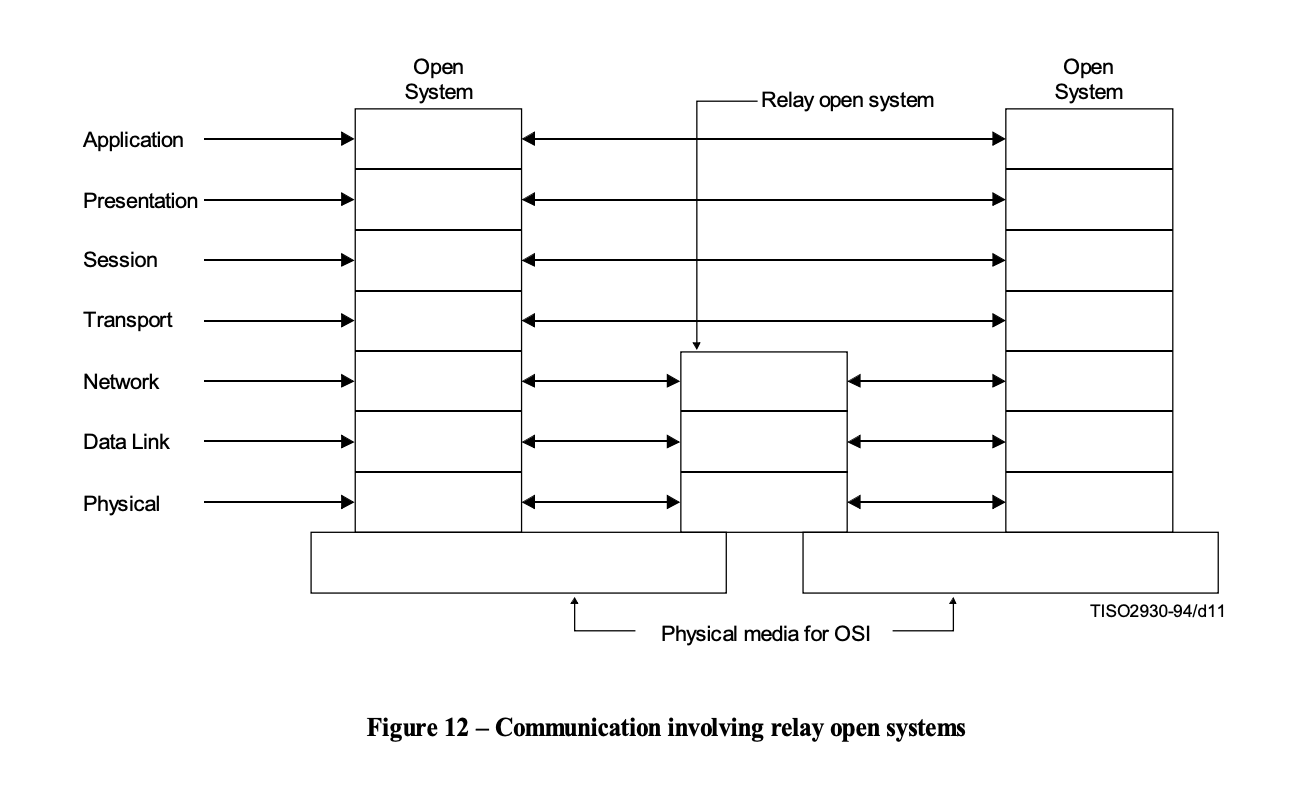
\includegraphics[width=.6\columnwidth]{Pictures/OSI.png}}
\caption{Extrait du standard ITU-T Rec. X.200 (1994 E)}
\end{wrapfigure}

Vous connaissez sûrement le principe d'empilement protocolaire dans les réseaux. Chaque protocole fournit un service et se base sur celui de la couche inférieure pour le réaliser. Le modèle d'origine définit sept couches pour transporter les données d'une application, n'importe où dans le monde.
  Les protocoles réseaux sont empilés les uns sur les autres, ceux du dessus utilisent les services offerts par ceux d’en dessous pour acheminer la donnée. Cela a donné lieu au modèle de référence de l’\ac{ISO} qui structure les réseaux depuis les années 1970. En théorie, il y a 7 \Index{couches}, mais l'internet a fait évoluer ce modèle et les numéros des couches, associés à des fonctionnalités, sont restés ; ce qui peut conduire à une numérotation étrange.
  
 \begin{figure}[tbp]
\centerline{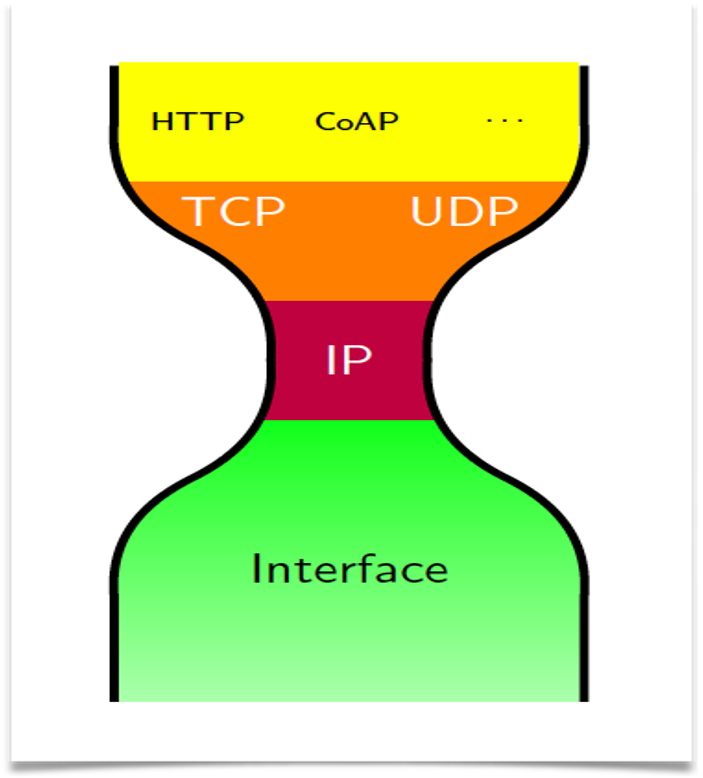
\includegraphics[width=.5\columnwidth]{Pictures/hourglass.png}}
\caption{Empilement protocolaire de l'Internet}
\label{fig-hourglass}
\end{figure}

  \vspace{1em}

\begin{wrapfigure}{r}{3cm}
\Youtube{https://youtu.be/vQ7zMVrqHbA}
\end{wrapfigure}

  L'internet a simplifié cette architecture (cf. figure~\vref{fig-hourglass}). C'est pour ça que l'on retrouve moins de couches et que les numéros ne sont pas contigus. 
  
  
    \vspace{1em}

  Les deux premières couches  en partant du bas, regroupées sous le nom d'Interface, permettent de transmettre les données binaires sur un support physique. La couche 1 s’occupe de cette modulation sur un support physique particulier (fibre optique, paire de cuivre, onde radio). La couche 2 regroupe les mécanismes qui permettent de structurer cette donnée sous forme de bloc de taille finie appelées trames, de définir les méthodes d’accès, c’est-à-dire quand l’équipement peut émettre, et les formats des adresses utilisées pour identifier les équipements. Ethernet ou Wi-Fi sont des exemples de protocoles de niveau 2 (qui intègrent leur niveau 1).

\begin{itemize}
\item l’\ac{IEEE} qui propose des standards comme Ethernet pour les réseaux filaires ou Bluetooth et Wifi pour les réseaux radio,
\item le \ac{3GPP}  qui opère au même niveau et définit les protocoles pour la téléphonie cellulaire (4G),
\item \ldots
\end{itemize}

  
    \vspace{1em}

  
  
  Au-dessus, on a le protocole \ac{IP} standardisé par l'IETF.  Le protocole \ac{IP} s’adapte simplement à tout moyen de communication. \ac{IP} propose ainsi une abstraction des moyens de communication aux couches applicatives, rendant l’accès au réseau et l’adressage universels. Le traitement dans les \Index{routeur}s (équipements chargés d’aiguiller l’information dans le réseau) doit être le plus rapide possible pour traiter un maximum de paquets par seconde. De plus, \ac{IP} ne spécialise pas le réseau pour un service ou un autre ; il ne fait qu’aiguiller les paquets vers la bonne destination. Le réseau Internet est un réseau mondial construit autour de ce protocole permettant potentiellement d'atteindre tous les équipements qui y sont connectés. 
  
  
  Les experts de l'internet aiment cette représentation en \Index{sablier} où \ac{IP} apparaît en position centrale mais est plus petit comparé aux autres protocoles. Par conception, \ac{IP} est très simple ; à la fois pour être portés facilement sur de nombreux niveaux 2 et être facilement utilisable par les couches hautes, mais également pour traiter les données très rapidement dans les nœuds d'interconnexion. 
  
  \ac{IP} est mis en oeuvre partout sur Internet aussi bien dans les équipements en extrémité du réseau que dans les routeurs chargés d'envoyer les données vers la bonne destination.
  
  
    \vspace{1em}

  Au-dessus on trouve deux protocoles qui ne sont mis en oeuvre que dans les équipements d'extrémité.  Si le niveau 3 permet de joindre une machine, le niveau 4 va permettre d’identifier l'application qui doit traiter les données. Les "adresses" de ces applications sont des numéros compris entre 1 et 65535 appelés \Index{port}s. Par exemple, les serveurs Web utilisent le port numéro 80 ou le numéro 443. 
  
  
  Le protocole \ac{TCP} va surveiller les données transférées et sera capable de retransmettre des données perdues, ralentir ou accélérer le transfert de données s’il détecte une saturation du réseau. En revanche, sa mise en œuvre est complexe et coûteuse en mémoire. Dans les cas simple, \ac{UDP} est préféré ; il n'apporte pas de traitement supplémentaire \ac{UDP}, c'est un protocole minimal qui se contentent d'aiguiller les données vers la bonne application sans aucun autre contrôle.
  

    \vspace{1em}

  
  Au-dessus, on trouve les applications qu'historiquement on classe dans la couche 7. Les applications sont très nombreuses mais la plus répandue est \ac{HTTP} qui sert à transporter les pages web, mais également elle permet des communications directes entre ordinateurs. 
  
  
    \vspace{1em}


   \begin{figure}[tbp]
\centerline{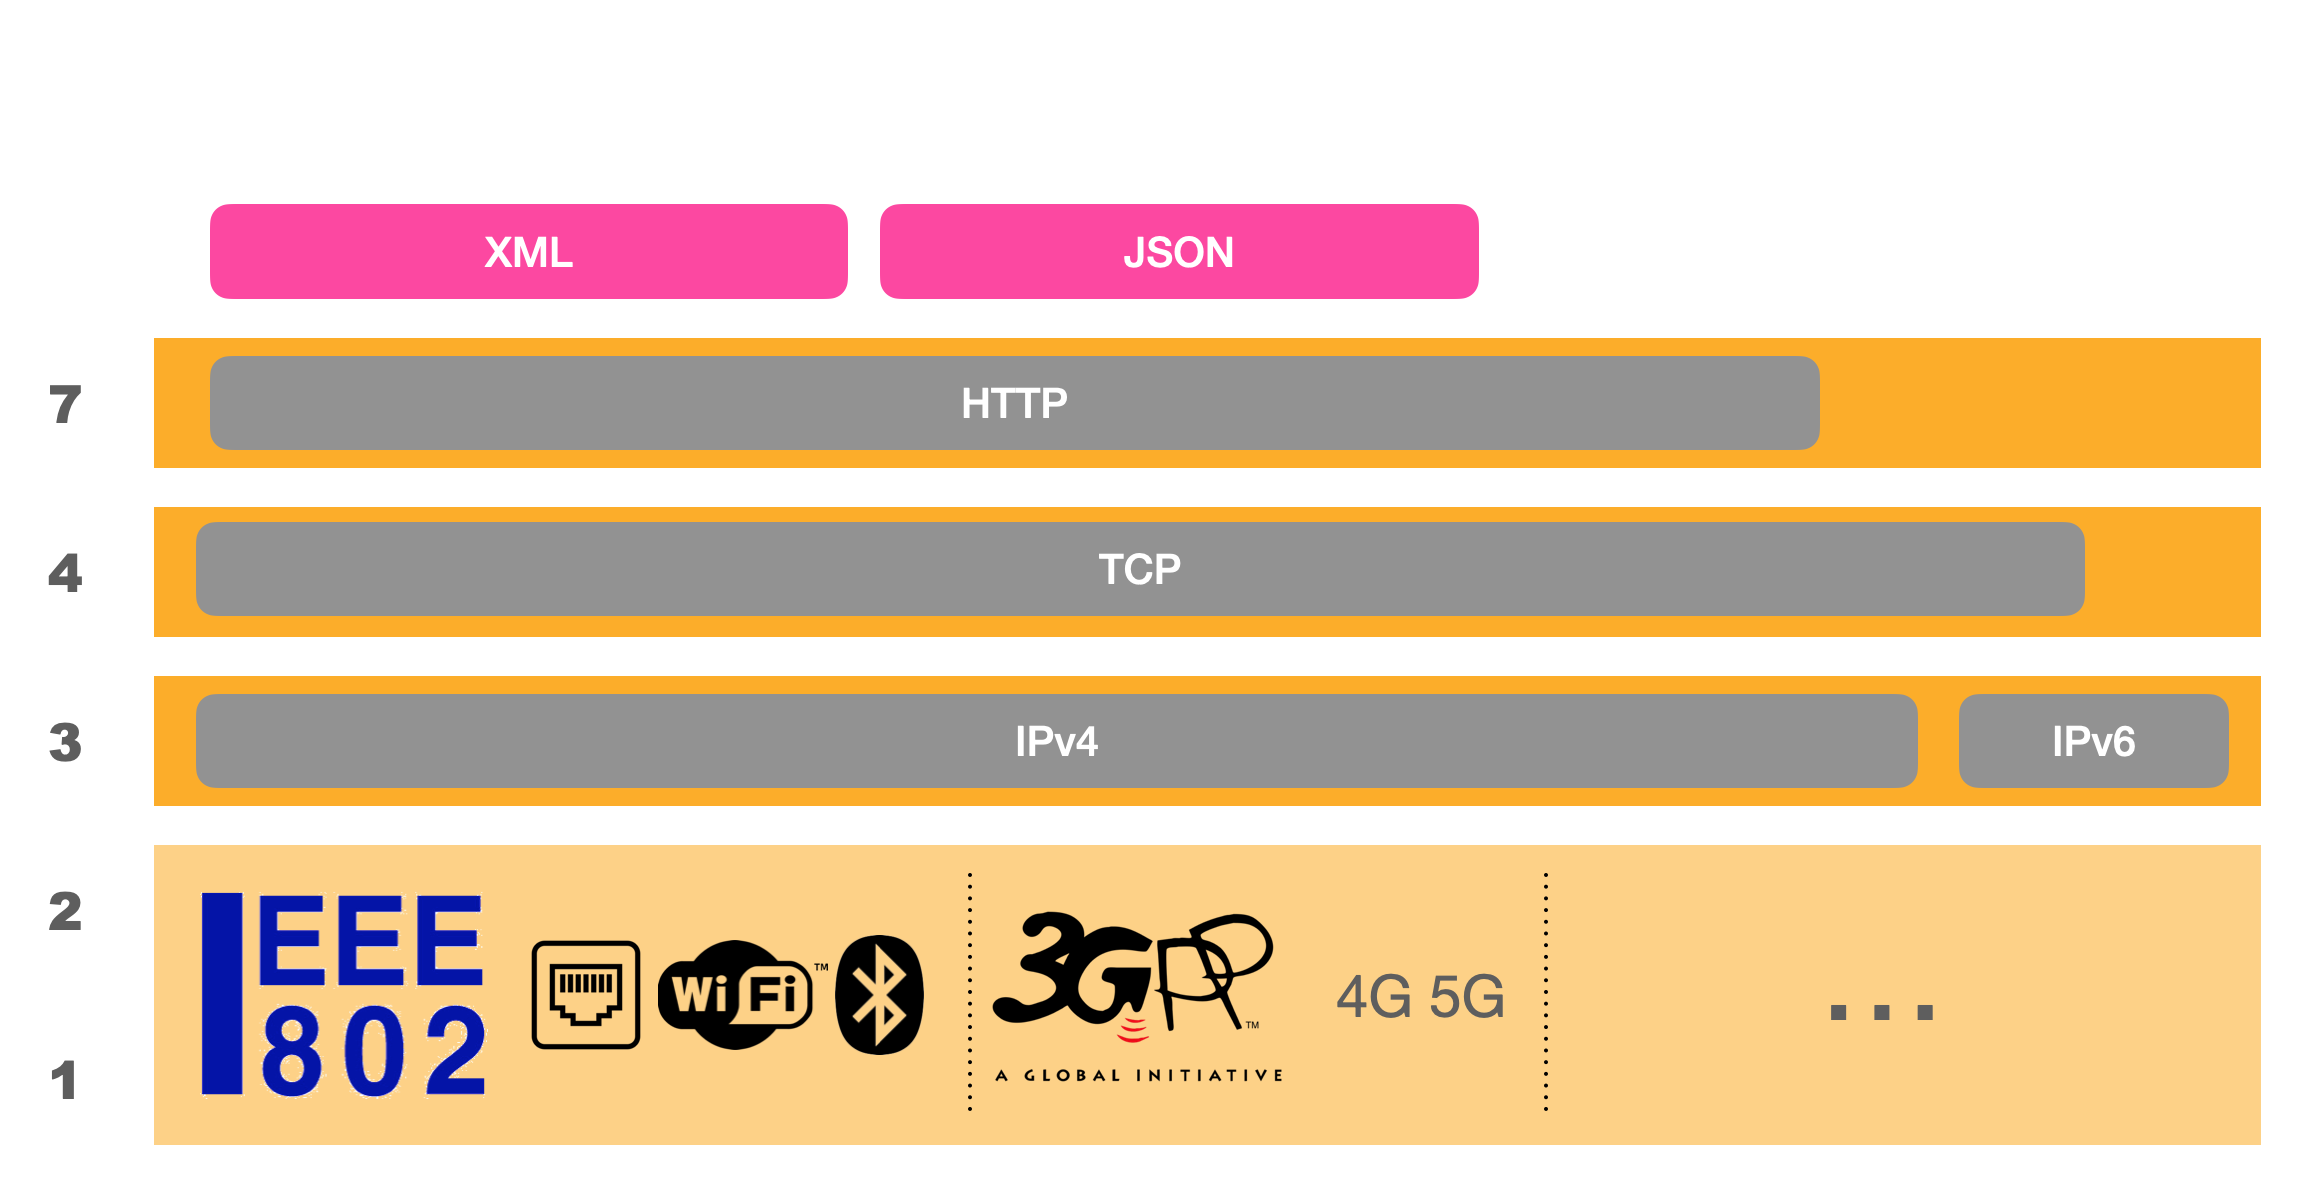
\includegraphics[width=1\columnwidth]{Pictures/fullIPstack.png}}
\caption{Principaux protocoles de l'Internet}
\label{fig-fullstack}
\end{figure}

  Pour le grand public, l’internet désigne surtout la totalité de cet assemblage protocolaire et est souvent confondu avec l’application qui a démocratisé son usage : le Web.  C'est vrai également pour les techniciens, le trafic produit par le Web est largement présent dans l'Internet. Ce schéma, figure~\vref{fig-fullstack} reprend la pile protocolaire majoritairement utilisé dans l'internet. On voit qu'au niveau 3 on a deux versions du protocole \ac{IP} ; la version 4 est la version historiquement déployée et elle a eu tellement de succès qui est de plus en plus difficile d'avoir des adresses \ac{IPv4} pour les machines. Pour permettre au réseau de continuer de fonctionner, une nouvelle version a été développée. \ac{IPv6} rend l'adressage quasi infini avec des adresses sur 128 bits. \ac{IPv6} gagne petit à petit du terrain dans les usages classiques et c'est surtout une brique essentielle pour l'internet des objets. 
  
  Le Web utilise majoritairement le protocole \ac{HTTP}. Et comme \ac{HTTP} repose sur \ac{TCP}, ces deux protocoles sont dominants sur le réseau. 
  
  Finalement ce graphique ajoute une couche supplémentaire, au-dessus de la couche 7, pour indiquer comment les données transportées sont structurées avec des formats comme \ac{XML} ou \ac{JSON} que nous verrons dans la suite.
  
  
  \Question{Pile Protocolaire}
  {Dans la pile protocolaire de l'internet, quels protocoles ont pour fonction d'aiguiller les paquets jusqu'à leur destination (2 réponses) 
  \begin{multicols}{4}
  \begin{itemize}[label=$\square$]
   \item \Wrong{Ethernet}
   \item \Wrong{IEEE}
   \item \Wrong{802.15.5}
   \item \Wrong{Wi-Fi}
   \item \Correct{IPv4}
   \item \Correct{IPv6}
   \item \Wrong{UDP}
   \item \Wrong{TCP}
   \item \Wrong{MQTT} 
   \item \Wrong{HTTP}
   \item \Wrong{CoAP}
   \item \Wrong{XML}
   \item \Wrong{JSON}
  \end{itemize}
  \end{multicols}
  }
  {Le protocole \ac{IP} permet de transporter l'information d'un bout à l'autre du réseau en utilisant les adresses \ac{IP} contenues dans les paquets. Il existe deux versions de ce protocole \ac{IPv4} initialement déployé et \ac{IPv6} qui offre beaucoup plus de capacité d'adressage.}
  
  \section{Les fondements du Web}
  
    \vspace{1em}
\begin{wrapfigure}{r}{3cm}
\Youtube{https://youtu.be/PKKzV-Vy33s}
\end{wrapfigure}

  L'architecture qui a conduit au Web est une formidable source d’inspiration pour le développement de nouveaux services car il est l’un des plus grands succès reposant sur le réseau Internet. Le Web forme de grands systèmes distribués et repose sur plusieurs principes qui le rendent universel et évolutif. La navigation avec un navigateur n’est que la partie visible du trafic ; les principes du web sont également utilisés pour le streaming vidéo, les échanges entre ordinateurs. 
  
  Le Web et ses extensions sont basés sur un modèle client-serveur. Les serveurs possèdent des ressources et les clients peuvent y accéder ou les modifier grâce à un protocole tel que \ac{HTTP}. Le modèle client-serveur est quelque chose de courant dans les réseaux informatiques, mais le Web suit certaines directives de conception connues sous le nom de \ac{REST}.

    \vspace{1em}

Selon Roy Fielding, qui a défini ce modèle~\cite{rest}, \ac{REST} est un ensemble de principes, de propriétés et de contraintes. \ac{REST} utilise le modèle de communication client-serveur et utilise généralement le protocole \ac{HTTP}.

Le principe \ac{REST} permet de concevoir des serveurs évolutifs. Un serveur doit être sans état, ce qui signifie qu’il ne conserve pas d’information après avoir répondu à une demande d’un client. Cela permet de simplifier le traitement dans le serveur qui doit traiter les requêtes d'un grand nombre de clients. 

Cela impose que l’état soit situé du côté du client. Cet état est alimenté à partir des données structurées que le client reçoit du serveur. Ainsi, lorsqu’un client demande une page Web, celle-ci peut contenir d’autres \ac{URI} pour la compléter, par exemple des images, des feuilles de style, des scripts, etc.

Le client doit donc comprendre les données que le serveur lui envoie et donc connaître le format de représentation de la ressource qu'il reçoit pour y retrouver les \ac{URI}. Donc, en plus de la ressource elle-même, le serveur ajoute des informations complémentaires, appelées métadonnées. Elles intègrent entre autres le format du contenu (content format). Il peut s’agir de texte pur, d’une image ou d’un format de texte structuré tel que \ac{HTML} ou \ac{JSON}.
  
      \vspace{1em}

\subsection{Ressources}

    \vspace{1em}

   \begin{wrapfigure}{r}{9cm}
\centerline{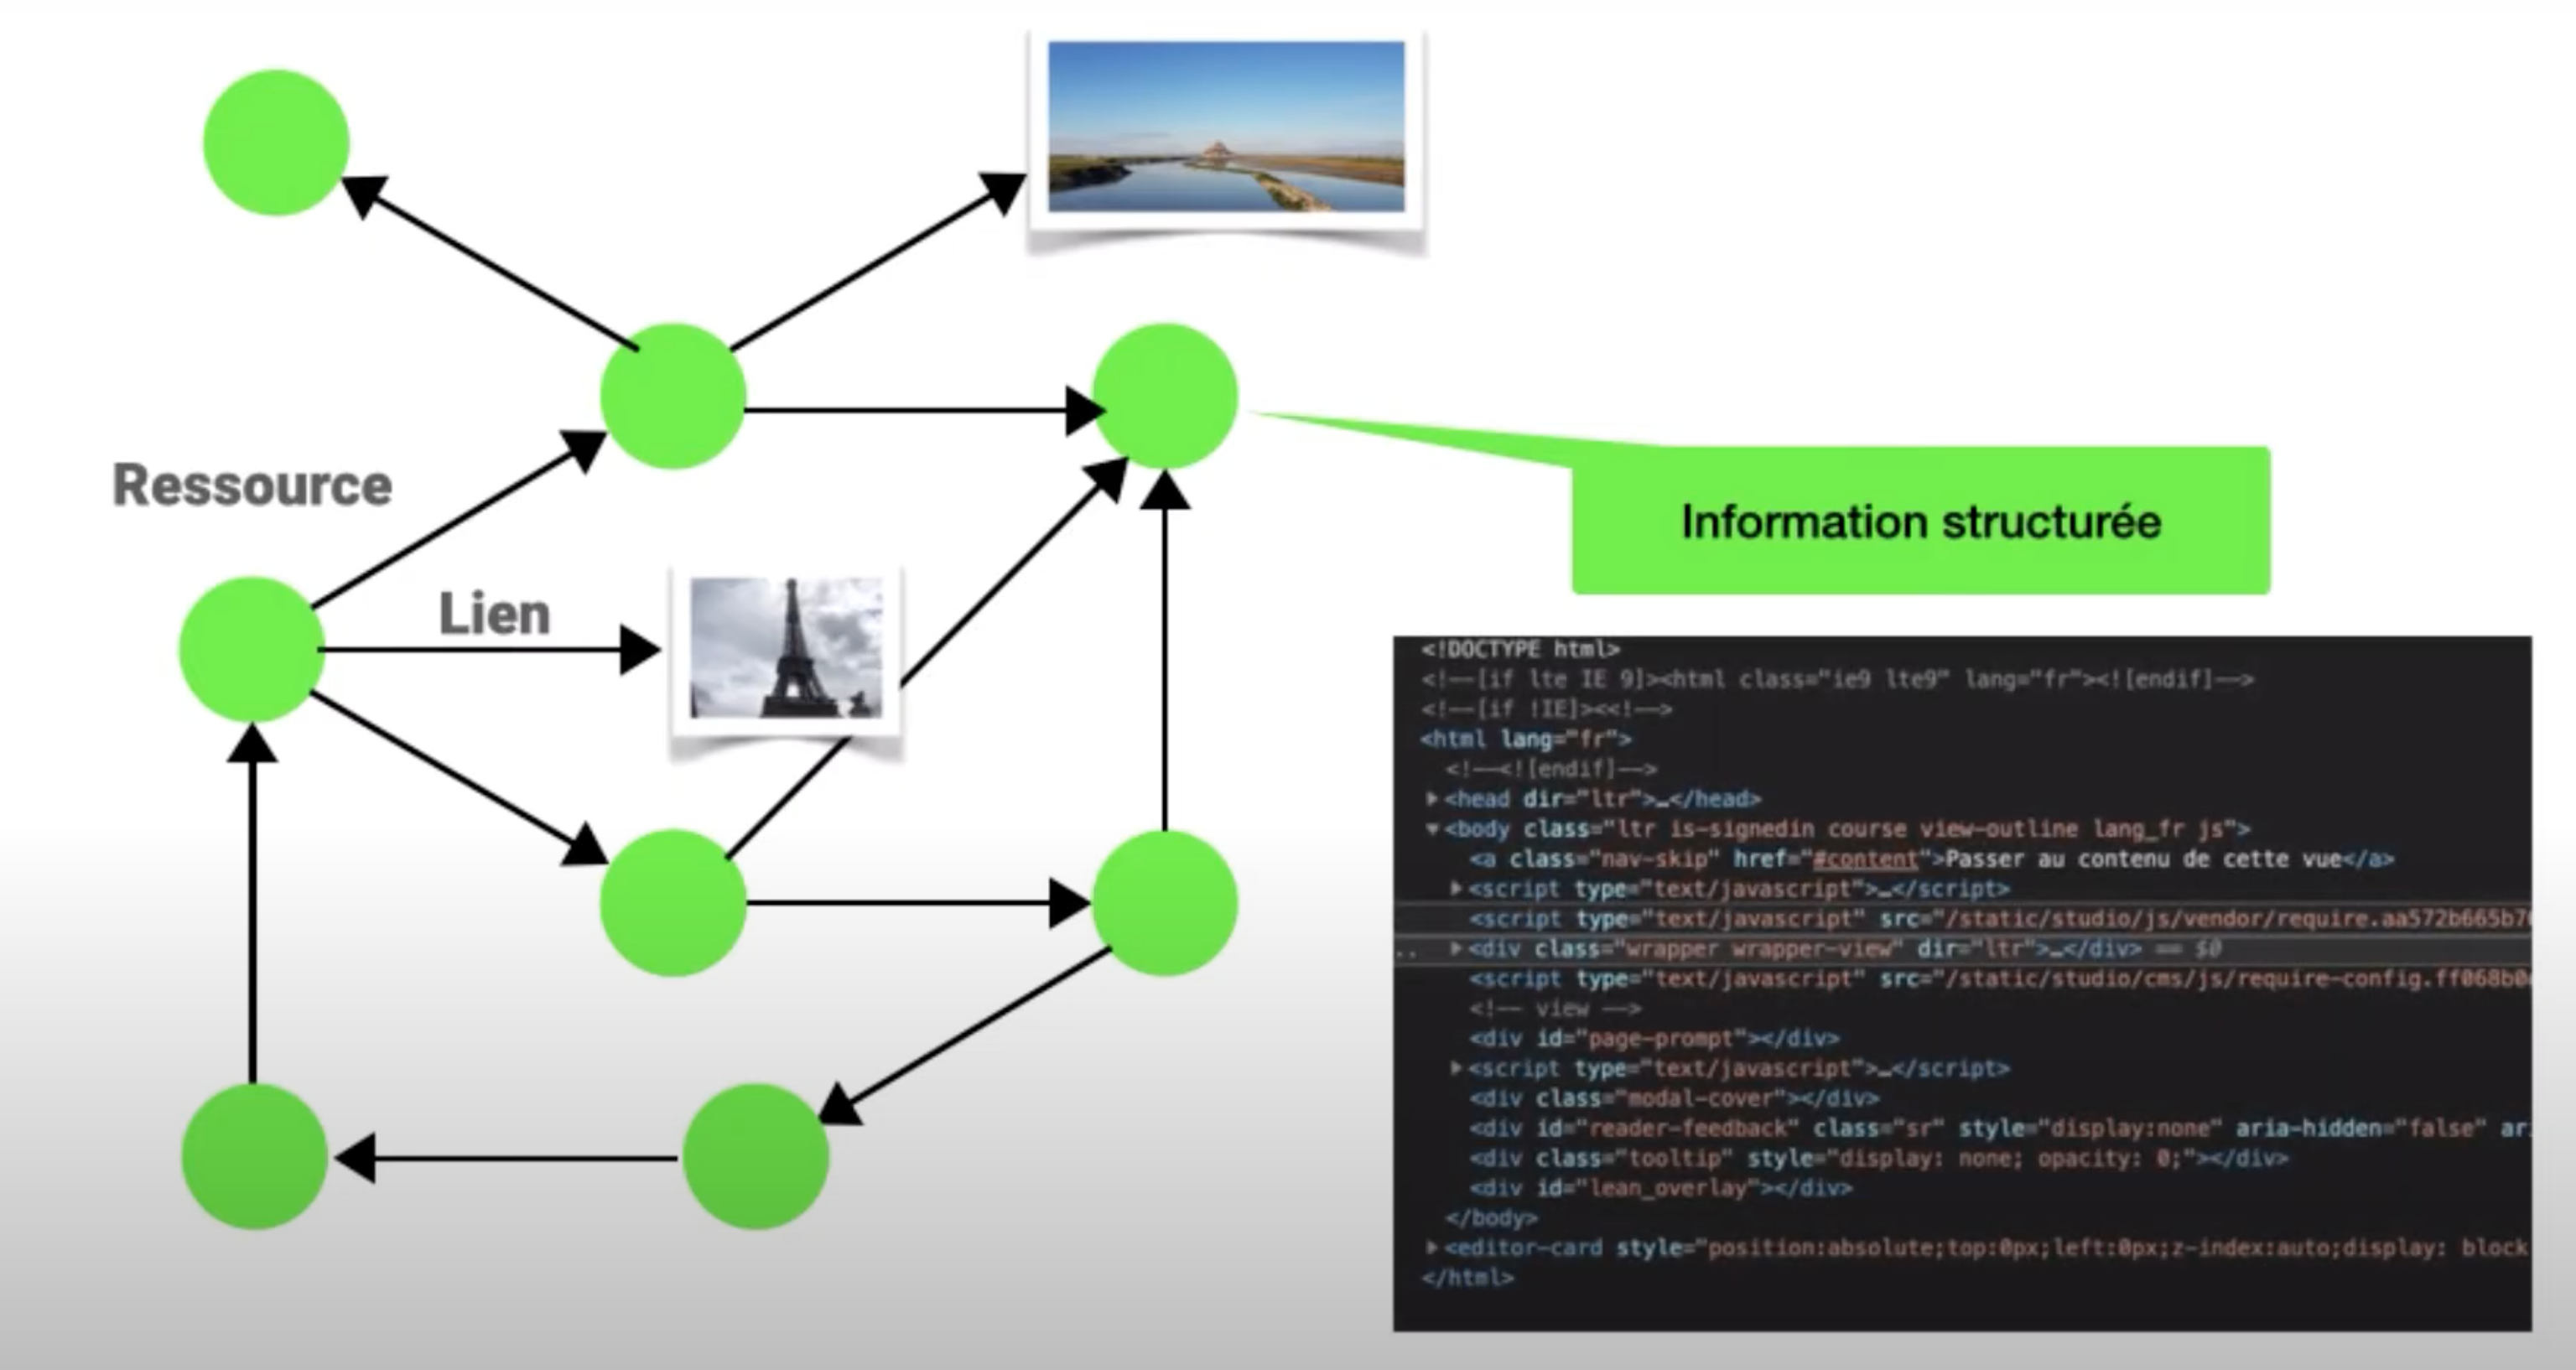
\includegraphics[width=.6\columnwidth]{web.png}}
\end{wrapfigure}
   L'élément de base est la ressource que l'on peut définir comme un bloc de données de taille finie. Les ressources peuvent elles-mêmes contenir des références à d'autres ressources qui à leur tour vont faire référence à d'autres ressources etc. etc. Cela forme un maillage entre ressources qui est comparé à une toile d'araignée (web en anglais). La ressource peut être, par exemple, une image dans ce cas elle ne fera pas référence à autre chose. Pour faire référence à une autre ressource, son contenu doit être structuré et doit donc être défini dans un format où l'on peut facilement comprendre qu'une partie du contenu est une référence a une autre ressource. HTML est un de ces langages qui permet aux pages web de se référencer entre elles par le biais de liens. 
  
      \vspace{1em}

\subsection{identifiants} 

    \vspace{1em}

   
   Chaque ressource du Web est identifiée par une valeur unique appelée \ac{URI}. Si l’URI contient des caractères internationaux, (comme les lettres accentuées, ...)   il est appelé \ac{IRI}.

Les \ac{URI} permettent de désigner une ressource de manière non ambiguë, c'est-à-dire que l'on ne retrouvera pas le même \ac{URI} pour désigner deux ressources différentes.  Par construction, la structure de l’\ac{URI} est hiérarchique, ce qui permet de créer des identificateurs uniques de manière distribuée. Si vous voulez identifier une ressource, vous devez posséder une séquence unique : un numéro de téléphone, un numéro de sécurité sociale, un nom de domaine. En y ajoutant quelque chose d'unique pour nous, cela crée un identifiant globalement unique. 

Par exemple, pour identifier une image, on peut la nommer

\begin{termc}[backgroundcolor=\color{palerod}, language=json, basicstyle=\ttfamily, escapechar=@]
image
\end{termc}

\noindent

mais il y a peu de chance que ce nom soit unique, d'autres personnes sur Terre ont sûrement eu la même idée. En revanche, si je la fais précéder de mon numéro de téléphone

\begin{termc}[backgroundcolor=\color{palerod}, language=json, basicstyle=\ttfamily, escapechar=@]
33667789078image
\end{termc}


\noindent
 sera unique si je ne nomme qu'une seule ressource "image". Un autre utilisateur sur le même principe pourra nommer sa ressource :

\begin{termc}[backgroundcolor=\color{palerod}, language=json, basicstyle=\ttfamily, escapechar=@]
33667239018image
\end{termc}


\noindent
sans ambiguïté possible. Cependant, comme le numéro de téléphone est unique dans l'espace des numéros de téléphone, d'autres numéros uniques pourraient entrer en conflit dans d'autres espaces de numérotation. 

Pour éviter les conflits, il est intéressant de donner, au début l'espace de numérotation, par exemple :

\begin{termc}[backgroundcolor=\color{palerod}, language=json, basicstyle=\ttfamily, escapechar=@]
tel:33667789078image
\end{termc}

\noindent
et

\begin{termc}[backgroundcolor=\color{palerod}, language=json, basicstyle=\ttfamily, escapechar=@]
ss:33667789078image
\end{termc}


\noindent
Les deux identifiants seront uniques, même si le hasard a fait que ce numéro de téléphone et ce numéro de sécurité sociale coïncident.

      \vspace{1em}


Les \ac{URI} formalisent ce principe. Le \rfc{3986} explique comment ils peuvent être construits. Un URI commence par un schéma indiquant l’autorité de nommage, suivi d’une valeur d’autorité puis d’un chemin dans l’espace d’autorité. Des caractères comme les ":" ou les "/" sont utilisés pour améliorer la lisibilité de l'\ac{URI}.



Par exemple~:

\begin{termc}[backgroundcolor=\color{palerod}, language=json, basicstyle=\ttfamily, escapechar=@]
mailto:mduerst@ifi.unizh.ch
ssh://utilisateur@example.com
ftp://ftp.is.co.za/rfc/rfc1808.txt
\end{termc}


      \vspace{1em}

Ainsi, si je mets une ressource sur un site Web, celui-ci est identifié par un nom de domaine, par exemple \texttt{example.com}. Je suis propriétaire de ce nom. Je peux donc l’utiliser pour identifier de manière unique ma ressource. Si on reprend le principe de construction d’un URI, j’aurai :

\begin{termc}[backgroundcolor=\color{palerod}, language=json, basicstyle=\ttfamily, escapechar=@]
http://example.com/ma_ressource
\end{termc}


Personne d’autre dans l’univers ne pourra identifier ses ressources avec cette chaîne de caractères puisque \texttt{example.com} m’appartient. Je dispose donc d’un espace de nommage infini qui me permet de désigner l’ensemble infini de ressources sans que personne d’autre ne puisse prendre les mêmes noms. Un \ac{URI} est une construction administrative permettant d’attribuer un identifiant unique global à une ressource spécifique.


  \begin{figure}[tbp]
\centerline{
\includegraphics[width=1\columnwidth]{Pictures/Capture15.png}}
\caption{Structuration d'une URI}
\label{fig-stucURI}
\end{figure}

L’\ac{URI} (cf.figure~\vref{fig-stucURI}) a pour but de facilement nommer une ressource, de pouvoir lier les ressources entre elles pour former cette toile d’araignée mondiale. Le schéma définit à la fois l'espace de nommage de l'autorité et son format. Une adresse \ac{IP} ou un nom de domaine comme autorité est à la fois un moyen d'assurer l'unicité globale, mais également de savoir comment accéder à la ressource. 

      \vspace{1em}

   Par exemple, \Index{spotify} a défini son propre schéma et ensuite il n'a plus besoin d'autorité mais structure le chemin pour référencer une playlist. 
   
   
   
   Tous les livres ont un numéro \ac{ISBN} qui permet d'identifier. Il peut être intégré aussi dans une URI. Il faut voir que ces deux types d'identifiants permettent de référencer un objet unique mais rien qu'en le lisant on ne peut pas accéder à la ressource. On appelle cette sous famille des \ac{URI}, des \ac{URN}. Si en revanche, en lisant l'URI on peut localiser la ressource on a une \ac{URL}.

Un sous-ensemble d’\ac{URI} peut être directement utilisé pour localiser la ressource, c’est-à-dire trouver sur quel serveur se trouve la ressource et comment y accéder. Il s’agit d’une URL bien connue du grand public et utilisée par les navigateurs Web.

Le schéma http est bien pratique car il peut se lire également comme un \ac{URL}. Ce schéma donne~:

\begin{itemize}
\item le protocole à utiliser pour accéder à la ressource (http),
\item l’autorité qui indique l’adresse du serveur (et son port),
\item et enfin, le chemin d’accès de ce que l'on va demander au serveur et qui peut parfois correspondre à une arborescence de fichiers sur un serveur.
\end{itemize}
   
   
       \vspace{1em}

  Mais il faut bien voir que le but initial est de faire un identifiant unique. Le schéma https donne la manière dont sera construit la suite et dans un second temps uniquement sera vu comme le protocole à utiliser pour accéder à la ressource. L'autorité est unique et dans un second temps servira à localiser le serveur. Et finalement le chemin va indiquer comment parvenir à accéder à la ressource sur le serveur. Donc les ressources de notre toile d'araignée mondiale sont présentes sur des serveurs et chaque ressource possède un identifiant unique. Dans un premier temps, le client connaît l'\ac{URI} d'une ressource. Si c'est une \ac{URL}, il peut contacter le serveur. Le serveur lui retourne la ressource. Le client l'analyse et découvre les \ac{URI} qu'il contient. Il peut donc interroger le ou les autres serveurs pour reconstruire localement une partie de la toile nécessaires au traitement que le client veut effectuer.
  
         \vspace{2em}

\Question{Unicité}{Qu'est ce qui est unique dans le monde (6 réponses) ?
\begin{itemize}[label=$\square$]
\item \Wrong{Un prénom.}
\item \Wrong{Un nom de famille.}
\item \Correct{un numéro de sécurité sociale utilisé en France.}
\item \Correct{un numéro de passeport.}
\item \Correct{un numéro de téléphone portable avec son préfixe international.}
\item \Correct{un numéro complet de compte en banque (\ac{IBAN}).}
\item \Wrong{l'adresse IP de ma machine dans mon réseau privé.}
\item \Correct{l'adresse IP d'un serveur fun-mooc (\texttt{51.255.9.16}).}
\item \Correct{le nom de domaine \texttt{plido.net}.}
\item \Wrong{le nom d'une ville.}
\end{itemize}}
{Ni le prénom, ni le nom de famille, ni leur combinaison ne forment des séquences uniques comme le dirait Jean Dupont.
Les numéros de passeport, de sécurité sociale, de téléphone, de compte bancaire sont par construction uniques dans leur espace, mais il pourrait y avoir des recouvrements. C'est pour cela qu'il faut indiquer la source ou l'autorité qui l'a alloué pour garantir l'unicité. Pour le passeport, l’autorité est le pays qui l’a produit. Le numéro de sécurité sociale correspond au numéro d'inscription au  \ac{RNIPP} (cf. \url{https://www.service-public.fr/particuliers/vosdroits/F33078}). Le code du pays pour le numéro de téléphone est attribué par l'UIT puis chaque opérateur a sa zone de numérotation. Pour le compte bancaire, c’est bien sûr la banque ; chaque banque ayant son propre code contenu au début de l'\ac{IBAN}.
L'adresse IP dans un réseau privé n'est pas unique. Le \rfc{1918} définit des plages d'adresses que tout le monde peut utiliser localement. Pour sortir sur Internet, il faut un dispositif spécial, appelé \ac{NAT}, qui va convertir l'adresse privée en une adresse publique qui, elle, est unique dans le monde. Les serveurs doivent être dans cet espace public et ont donc une adresse unique dans le monde.
Les noms de domaines sont uniques dans le monde par construction mais il peuvent être partagés par plusieurs utilisateurs. On peut donc les étendre comme \texttt{machine1.plido.net}, \texttt{machine2.plido.net}... ou, s'il s'agit de la même machine, ajouter un numéro de port après pour indiquer le service : \texttt{www.plido.net:80}, \texttt{www.plido.net:8080}.
Quant au nom d'une ville, il n'est pas unique. Il faut aussi préciser le pays, voire la région.
}
 

  \subsection{Interactions}
  
         \vspace{1em}

  Les interactions entre clients et serveurs sont très simples. Le client va gérer les interactions avec les ressources sur un serveur. Il peut, par exemple, récupérer une ressource grâce à une méthode \Index{GET}. Il peut également écrire les données dans une ressource existante grâce à une méthode \Index{PUT}. 
  
  Le nombre d'interactions est très limité. \ac{HTTP} ou \ac{HTTPS} est un moyen de mettre en oeuvre ces méthodes. 




\ac{HTTP} est un protocole qui peut être utilisé pour mettre en œuvre un serveur Web les principes de \ac{REST} (qualifié en anglais de \Index{RESTfull}). \ac{HTTP} définit différentes méthodes permettant au client d’interagir avec les ressources sur le serveur~:

\begin{itemize}
    \item \Index{GET} est utilisée pour récupérer la représentation d’une ressource (par exemple page Web, valeur de température d’un capteur, etc.). Par exemple, la figure~\vref{fig-GET} donne le format d’en-tête \ac{HTTP} GET pour récupérer une page Web :

 \begin{figure}[tbp]
\centerline{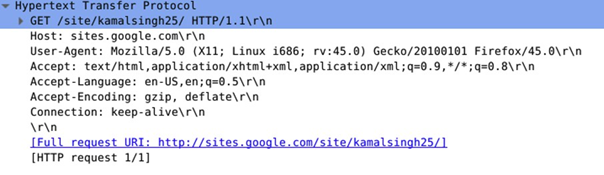
\includegraphics[width=1\columnwidth]{Pictures/GET.png}}
\caption{Contenu d'une requête HTTP GET}
\label{fig-GET}
\end{figure}

\item  \Index{HEAD} est utilisée pour récupérer uniquement les métadonnées présentes dans les en-têtes de réponse sans le corps de réponse ;
\item  \Index{POST} est utilisée pour indiquer au serveur une nouvelle ressource  ;
\item  \Index{PUT} est utilisée pour stocker une ressource à l’endroit identifié par l’\ac{URI} dans la requête. Si la ressource existe déjà, elle sera modifiée ;
\item \Index{PATCH} permet au client de ne modifier qu’une partie de la ressource ;
\item  \Index{DELETE} est utilisée pour supprimer la ressource définie.


\end{itemize}

 \Question{Etat}{Est-ce que le serveur garde un état des précédentes requêtes ?
\begin{itemize}[label=$\circ$]
\item \Wrong{Oui}
\item \Correct{Non}
\end{itemize}}
{Le serveur répond à une requête puis passe à la suivante. Il ne garde pas d'état. En revanche, une requête peut servir à modifier le contenu d'une ressource.}

\Question{Wold Wide Web}{Le World Wide Web est basé sur ce principe des états pour :
\begin{itemize}[label=$\circ$]
\item \Wrong{fonctionner à la fois sur des ordinateurs et des téléphones portables,}
\item \Correct{pouvoir servir un grand nombre de requêtes}

\item \Wrong{chiffrer les communications,}
\end{itemize}}
{Voir le commentaire précédent}

 \Question{Repésentation de l'Information}
  {Quels sont les formats qui permettent de représenter des informations structurées (2 réponses)~: 
  \begin{multicols}{4}
  \begin{itemize}[label=$\square$]
   \item \Wrong{Ethernet}
   \item \Wrong{IEEE}
   \item \Wrong{802.15.5}
   \item \Wrong{Wi-Fi}
   \item \Wrong{IPv4}
   \item \Wrong{IPv6}
   \item \Wrong{UDP}
   \item \Wrong{TCP}
   \item \Wrong{MQTT} 
   \item \Wrong{HTTP}
   \item \Wrong{CoAP}
   \item \Correct{XML}
   \item \Correct{JSON}
  \end{itemize}
  \end{multicols}
  }
  {Il s'agit de XML et JSON qui permettent d'envoyer des données stucturées. Les autres propositions indiquent des protocoles de transport de l'information de niveau 2, 3, 4 et 7.}
  
\Question{Schéma}{Dans l'URI \texttt{https://plido.net/unit/definition.html}, quel est le schéma ?\newline}
{\noindent\texttt{http}~: le Schéma indique comment sera construite l'URI}

\Question{Authorité}{Dans l'URI \texttt{https://plido.net/unit/definition.html}, quel est l'autorité ?\newline}
{\noindent\texttt{plido.net}~: il s'agit de la séquence globalement unique.}


\section {Modèle Publish/Subscribe}

Il existe d’autres formalismes que REST. Un autre formalisme, très populaire, est orienté "diffusion" en utilisant le principe ”publier/abonner” ou ”publish/subscribe”. Comme nous allons le montrer dans la suite, même si les fonctionnalités entre ces deux modes peuvent sembler similaires, la philosophie de conception est très différente : publish/subscribe vise des applications intégrées tandis que REST vise l’interopérabilité globale. 

Le modèle publish/subscribe fait le découplage entre l’expéditeur d’un message et son destinataire. Dans ce paradigme (cf. figure ci-dessous), il existe des ”Publishers” qui produisent des données ou des messages et envoient le message à une entité généralement appelée ”Broker”. En outre, les messages peuvent être classés en ”Topics”, contenus ou types, etc. Ensuite, il existe des abonnés qui souscrivent au broker, par exemple à un topic donné, afin de recevoir les messages qui les intéressent, comme montré dans le schéma.

Le broker peut alors utiliser des filtres pour envoyer uniquement ces messages aux abonnés du topic concerné. Il existe plusieurs protocoles Publish-Subscribe tels que MQTT (Message Queuing Telemetry Transport), AMQP (Advanced Message Queuing Protocol), JMS (Java Messaging Service) ou XMPP (Extensible Messaging Protocol et Présence).

\subsection{MQTT}

MQTT est détaillé dans la suite du cours car il est très populaire pour la communication entre processus, mais également dans l’internet des objets.

Imaginons par exemple que plusieurs capteurs soient installés dans deux bâtiments A et B. Certains capteurs collectent des informations sur la température et d’autres collectent des informations sur l’humidité. Ces capteurs peuvent envoyer les données régulièrement à un broker central.

Les données peuvent être classées en différentes rubriques qui peuvent également être organisées de manière hiérarchique. Par exemple, le topic /sensor signifie "toutes les données de capteurs", \texttt{/sensor/buildingA/} signifie "des données de capteurs uniquement installées dans le bâtiment A". En plus, \texttt{/sensor/buildingA/temperature} pourrait signifier "des données de capteurs de température installés uniquement dans le bâtiment A".

Certains abonnés peuvent s’abonner aux messages en fonction de leur intérêt. Ainsi, un abonné intéressé uniquement par les données d’humidité du bâtiment B peut s’abonner au sujet \texttt{/sensor/buildingB/humidity} et le broker n’enverra que ces données à cet abonné.

\subsection{différence avec REST}

Les principaux avantages du paradigme publish-subscribe par rapport au paradigme client-serveur, tels qu'inclus en REST, sont les suivants :
\begin{itemize}
\item faible couplage entre émetteur et récepteur, le broker sert d'intermédiaire et stocke les informations ;
\item passage à l’échelle. Les données provenant d'une source ne sont émises qu'une fois par la source. Le broker les recopie vers tous les abonnés. Dans un mode client/serveur, les données doivent être émises par le serveur autant que fois que les clients le demandent.
\end{itemize}
L’absence de couplage entre l’expéditeur et le destinataire se fait en termes d’espace, de temps et de synchronisation. Celui qui publie les données a une tâche simplifiée. Il n'a pas à gérer ou connaître ceux qui les consomment, il n'a qu’à les envoyer au broker.

MQTT est très léger et conçu pour les périphériques de faibles puissances. Il a une très petite empreinte logicielle et est optimisé pour fonctionner dans les environnements à faible bande passante. Cela rend MQTT idéal pour les applications IoT. Malgré tout, l’usage de TCP et des très nombreux acquittements peut s’avérer lourds pour les équipements ou les réseaux très contraints. Une version plus légère basée sur UDP existe pour ces cas d’usage, mais elle est peu utilisée.

S'ils se ressemblent, les principes de nommage des topics MQTT et des URI REST sont complètement différents. Par rapport à MQTT, le chemin dans l'URI n'a pas de sémantique. Il a juste vocation à être unique. Il ne peut pas être utilisé pour agréger plusieurs sources d'information. Si deux capteurs publient respectivement sur les topics \texttt{/sensor/buildingA/temperature} et \texttt{/sensor/buildingB/temperature}, un subscriber peut s'abonner au topic \texttt{/sensor/*/temperature} pour recevoir toutes les mesures ; ce qui est impossible avec REST : il faudra autant de requêtes que de capteurs pour récupérer l'ensemble des mesures.

Les URI sont simplement uniques au monde par leur construction alors que les topics du MQTT sont spécifiques à une application. Un topic MQTT peut être interprété différemment par deux applications différentes. Cela ne permet pas une interopérabilité sémantique. Les abonnés doivent être construits avec une connaissance des topics utilisés par les publieurs.

\cleardoublepage

\chapter {Wireshark}

\Index{Wireshark} va être notre ami dans la suite de cet ouvrage pour comprendre le fonctionnement des protocoles et analyser les données qui vont circuler. Malheureusement, dans certains cas, nous devons avoir recours à des outil plus rustiques comme des traces en \Index{hexadécimal}\footnote{\url{https://fr.wikipedia.org/wiki/Syst\%C3\%A8me\_hexad\%C3\%A9cimal}} (base 16).  Il faut donc se familiariser avec ces outils, ce que nous allons faire dare-dare en analysant des requêtes HTTP simples. Si vous avez accès à un ordinateur pouvant faire tourner Wireshark, nous vous recommandons d'essayer de faire les manipulation indiquées et de répondre aux questions.

\section{Installation}

L'installation de Wireshark se fait en allant sur le site éponyme \url{https://www.wireshark.org/}, soit sous Linux en installant le paquetage \texttt{wireshark}. Ce programme nécessite des droits particuliers pour accéder aux messages venant du réseau, il faut les accorder au moment de l'installation.

\section{Démarrage}

Si vous lancez Wireshark avec les bon privilèges, la fenêtre d'accueil va afficher les interfaces disponibles, comme le montre la figure~\vref{fig-wires-open} sur Windows. En regard avec le modèle de référence de l'\ac{ISO}, il s'agit des protocoles de niveau 2 présent sur l'ordinateur. Il peut s'agit d'une carte physique comme Ethernet ou Wi-Fi ou d'interface virtuelle utilisées pour communiquer en interne sur l'ordinateur. 

\begin{figure}[tbp]
\centerline{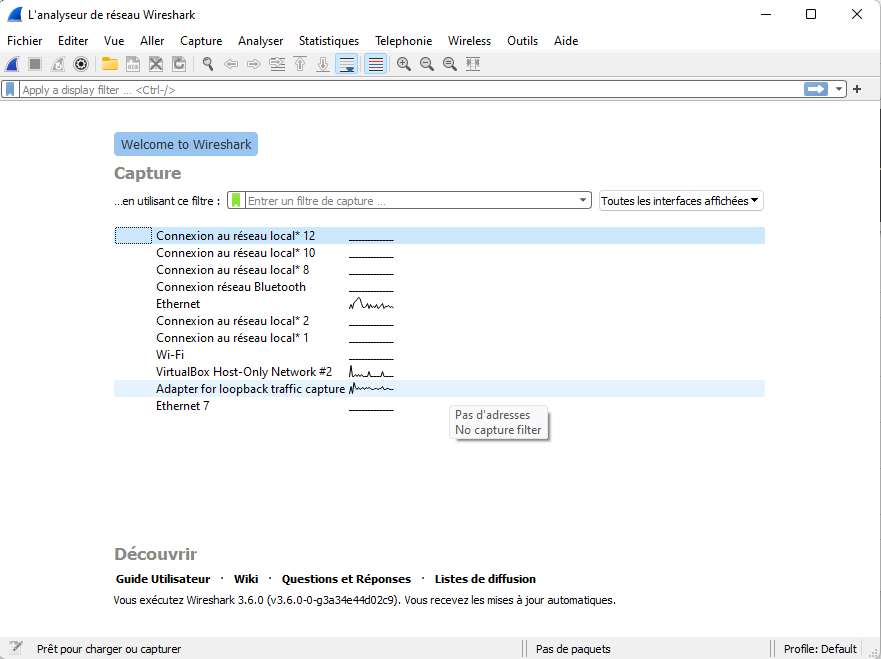
\includegraphics[width=1\columnwidth]{Pictures/wireshark-open.png}}
\caption{Ouverture de Wireshark}
\label{fig-wires-open}
\end{figure}


Il s'agit de déterminer quelle interface choisir. Ce n'est pas toujours facile car leurs noms ne sont pas toujours très explicites. Les petites courbes à gauche du nom indiquent le trafic instantané que Wireshark mesure. Sur le schéma, 3 interfaces sont actives : Ethernet, la communication avec une machine virtuelle et une interface appelée \textit{\Index{loopback}}.  La première permet d'avoir les communications avec l'extérieur et la dernière sera très utile lors des échanges entre deux processus dans cette machine.

\section {Capture}

En cliquant sur le nom de l'interface donnant accès au réseau exterieur (\index{Ethernet} dans notre cas), la fenêtre se découpe en 3 parties, comme le montre la figure~\vref{fig-wires-cap}.

\begin{figure}[tbp]
\centerline{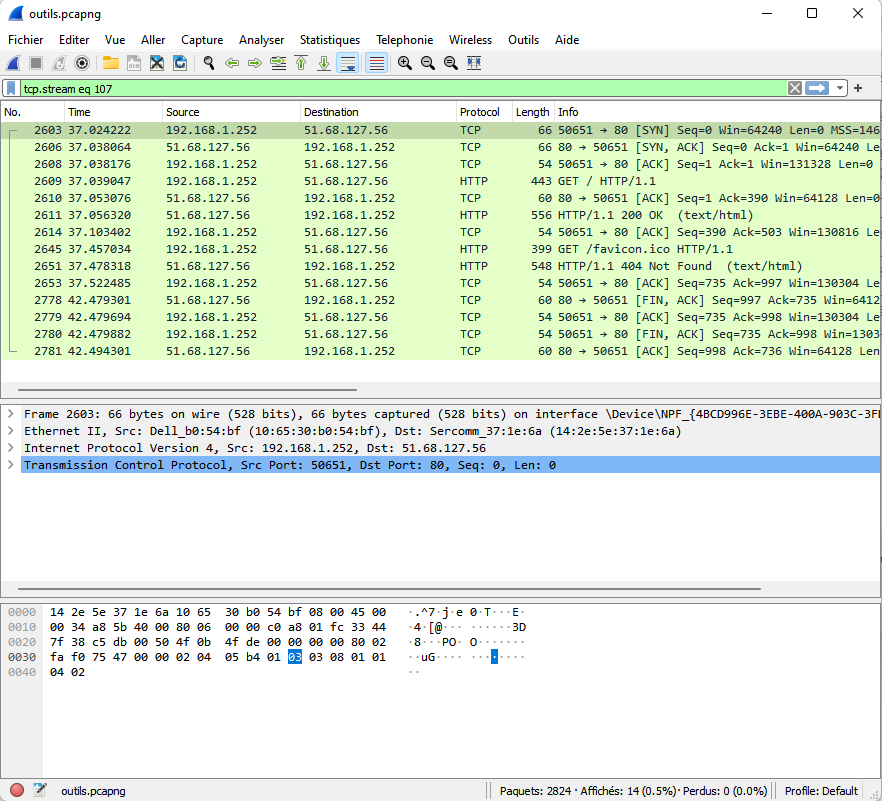
\includegraphics[width=1\columnwidth]{Pictures/ws-capture.png}}
\caption{Capture du trafic}
\label{fig-wires-cap}
\end{figure}

L'écran de Wireshark se divise en 3 parties :
\begin{itemize}
\item en haut, défile les trames qui sont capturées sur le réseau, chaque protocole à une couleur dédiée pour facilité le repérage~:
\begin{itemize}
\item le numéro de trame capturée, il s'agit d'une information ajoutée par Wireshark,
\item l'heure de capture de la trame. Cette information est aussi ajoutée par Wireshark,
\item l'adresse IP (IPv4 ou IPv6) de la machine à l'origine du paquet, 
\item l'adresse IP (IPv4 ou IPv6) de la machine destinataire du paquet,
\item le protocole de plus haut niveau contenu dans la trame. Dans notre cas, cela peut être TCP si le message TCP ne contient pas de données, comme lors de l'ouverture de connexion, ou de certains acquittements. On voit également les messages \ac{HTTP} qui sont bien entendu encapsulés dans TCP,
\item la taille en octets de la trame capturée par Wireshark,
\item finalement Wireshark fourni un résumé du contenu de la trame, pour comprendre ce qui se passe sur le réseau. Dans la capture, on retrouve pour les messages \ac{HTTP}, les requêtes GET ou les notifications ;
\end{itemize}
\item si une trame est sélectionnée dans la liste, elle apparaît dans la zone du milieu avec l'empilement protocolaire. Le contenu de chacun de ces protocoles peut être détaillé en cliquant sur le petit triangle à gauche ;
\item la fenêtre du bas donne l'équivalent en hexadécimal. Les parties surlignées correspondent aux champs sélectionnés dans la fenêtre du milieu. À noter que l'on retrouve l'information à la fois en hexadécimal et en caractère \ac{ASCII}, ce qui aide à la lecture quand on cherche une valeur spécifique.
\end{itemize}

\Question{Première colonne}
{Dans la première colonne~:
 \begin{itemize}[label=$\circ$]
   \item \Correct{Le numéro de la trame attribué par Wireshark à sa réception}
   \item \Wrong{Le numéro de la trame relevé directement dans la trame Ethernet}
  \end{itemize}
}
{
Ces numéros sont séquentiels, ils sont donc attribué localement par Wireshark. De plus il n'existe aucun champ de cette sorte dans Ethernet.
}
\Question{Deuxième colonne}
{Dans la deuxième colonne~:
 \begin{itemize}[label=$\circ$]
   \item \Correct{L'heure de réception par Wireshark}
   \item \Wrong{L'instant d'émission de la trame}
  \end{itemize}
}
{
Comme dans le cas précédent, ce numéro est ajouté par Wireshark, il n'existe pas de champ protocolaire indiquant l'instant d'émission.
}
\Question{Les troisième et quatrième colonnes}
{Dans les troisième et quatrième colonnes~:
 \begin{itemize}[label=$\circ$]
   \item \Wrong{les adresses Ethernet des machines.}
   \item \Wrong{Uniquement les adresses IPv4 des machines.}
   \item \Correct{Les adresses IPv4 ou IPv6 des machines.}
  \end{itemize}
}
{
Wireshark traite de la même manière les adresses IPv4 ou IPv6, elles sont donc affichées dans ces colonnes. L'adresse Ethernet (ou MAC) sur 48 bits n'est pas affichée par défaut dans cet écran.
}

\Question{La cinquième colonne}
{Dans la cinquième colonne~:
 \begin{itemize}[label=$\circ$]
   \item \Wrong{Le protocole applicatif (niveau 7).}
   \item \Correct{Le dernier (de plus haut niveau) protocole reconnu.}
   \item \Wrong{Le protocole de niveau 4 (ici TCP ou UDP).}
  \end{itemize}
}
{
Wireshark fournit l'information de plus haut niveau. Dans la figure~\vref{fig-wires-cap} certaines trames sont indiquées comme transportant le protocole HTTP, tandis que d'autres, généralement les acquittements sont indiqués comme étant de type TCP car elles ne transportent pas de données venant des couches supérieures.
}
\Question{La sixième colonne}
{Dans la sixième colonne~:
 \begin{itemize}[label=$\circ$]
   \item \Wrong{La taille en bits de la trame.}
   \item \Correct{La taille en octets de la trame.}
  \end{itemize}
}
{
L'unité est l'octet.
}
\Question{La septième colonne}
{Dans la septième colonne~:
 \begin{itemize}[label=$\circ$]
   \item \Correct{Un résumé des informations transportées par le protocole de plus haut niveau.}
   \item \Wrong{Les options d'IPv4.}
   \item \Wrong{le contenu en ASCII du message de plus haut niveau.}
  \end{itemize}
}
{
Wireshark cherche a interpréter les champs du protocole de plus haut niveau pour offrir un affichage synthétique de l'information.}
  \vspace{1em}

Cela fait beaucoup de trafic, nous allons limiter ce qui est affiché en ajoutant un filtre à un destinataire particulier. Le site \texttt{outils.plido.net} à l'adresse IPv4 \texttt{51.68.127.56}. Dans la fenêtre où il est indiqué \textit{Apply a display filter.} taper les instructions suivante: 

\begin{verbatim}
    ip.addr==51.68.127.56
\end{verbatim}

\noindent n'oubliez par le double \texttt{==} et la fenêtre doit devenir verte quand tout sera tapé indiquant que la syntaxe du filtre est correcte. En appuyant sur entrée, la fenêtre doit se vider.

\subsection{Analyse du trafic web}

Dans la barre d'adresse de votre navigateur préféré, taper l'URL suivante:

\begin{verbatim}
    http://outils.plido.net
\end{verbatim}

\noindent et la page Web indiqué figure~\vref{fig-firefox-hello} doit apparaître. 

\begin{figure}[tbp]
\centerline{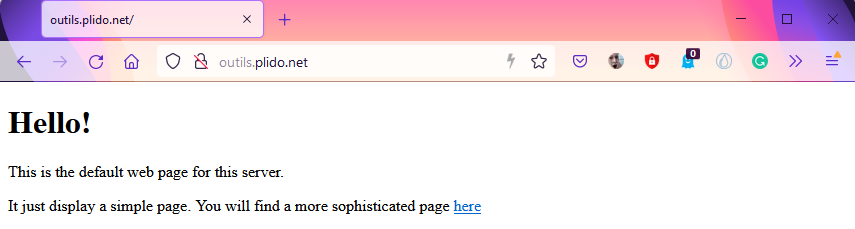
\includegraphics[width=1\columnwidth]{Pictures/firefox-simple.png}}
\caption{Afficher de la page par Firefox}
\label{fig-firefox-hello}
\end{figure}

  \vspace{1em}

Wireshark a permis de visualiser le trafic échangé entre l'ordinateur et le serveur Web. Le trafic doit être similaire a celui de la figure~\vref{fig-wires-cap}. La figure s'obtient en sélectionnant le menu \textit{Statistiques/Graphique de flux} et en cochant \textit{Limiter au Filtre d'Affichage}. Elle est un peu plus lisible car elle représente les échanges sous forme de chronographes.

\begin{figure}[tbp]
\centerline{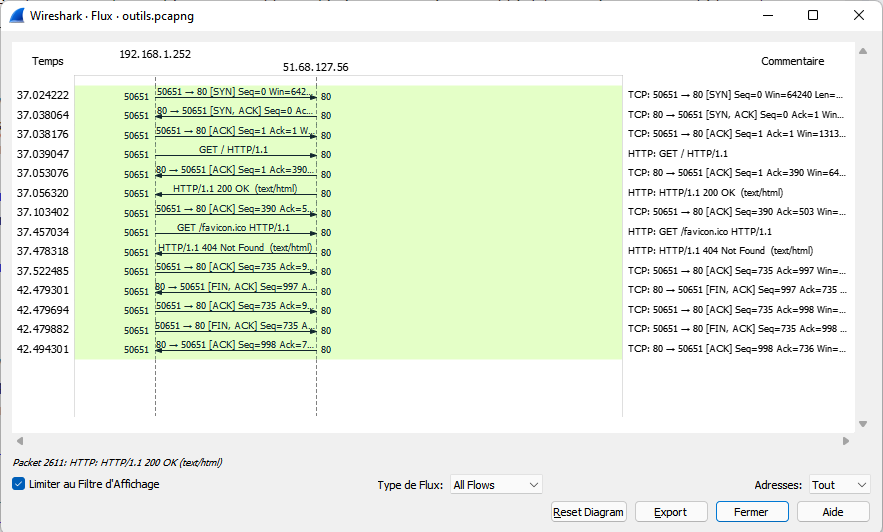
\includegraphics[width=1\columnwidth]{Pictures/ws-filtre.png}}
\caption{Diagramme temporel des échanges.}
\label{fig-ws-filtre}
\end{figure}

Trois phases peuvent être distinguées~:
\begin{itemize}
    \item L'ouverture de connexion TCP avec l'émission de trois messages TCP;
    \item la phase de transfert de données~:
    \begin{itemize}
        \item le client envoie une requête HTTP GET au serveur pour demander la ressource à la racine (\texttt{/}),
        \item le serveur acquitte le message au niveau TCP pour indiquer qu'il a bien été reçu.
        \item le serveur envoie la réponse à la requête précédente et précisant le statut (\textttt{200 : OK}) et le que contenu est formaté en HTML.
        \item le client acquitte ce message au niveau TCP
        \item le client envoie une nouvelle requête HTTP GET pour obtenir la ressource \texttt{/facicon.ico}
        \item le serveur répond que la ressource n'existe pas (\texttt{404 : Not Found}). Cette requête acquitte implicitement le message précédent.
        \item le client acquitte la réponse du serveur au niveau TCP.
    \end{itemize}
    \item le serveur termine la connexion après 5 secondes d'inactivité. La fermeture se fait en échangeant 4 messages TCP.
\end{itemize}

\Question{Code de notification de HTTP}
{Dans la trace suivante, nous avons vu que le serveur répondait aux requêtes du client par un numéro à 3 chiffres. A l'aide du \rfc{7231}, pouvez-vous attribuer le chiffre de gauche à une catégorie de notifications:
  \vspace{1em}

\tabto{3cm}
\begin{description}
    \item    0 $\square$ \tab\tab $\square$ Redirection 
    \item    1 $\square$ \tab\tab $\square$ Erreur coté serveur
    \item    2 $\square$ \tab\tab $\square$ Erreur coté client
    \item    3 $\square$ \tab\tab $\square$ Non attribué 
    \item    4 $\square$ \tab\tab $\square$ Succès
    \item    5 $\square$ \tab\tab $\square$ Information 
\end{description}

}
{
\begin{description}
    \item    0~:  Non attribué 
    \item    1~: Information 
    \item    2~: Succès
    \item    3~: Redirection
    \item    4~: Erreur coté client
    \item    5~: Erreur coté serveur
\end{description}}

\subsection{Analyse des requêtes HTTP}

La version 1.1 du protocole \ac{HTTP}  est spécifiée par le \rfc{7230}. Nous allons regarder une petite description en anglais de l'architecture et des formats des messages.

\begin{termc} [basicstyle=\footnotesize\ttfamily, frame=single]

2.  Architecture

  HTTP was created for the World Wide Web (WWW) architecture and has
  evolved over time to support the scalability needs of a worldwide
  hypertext system.  Much of that architecture is reflected in the
  terminology and syntax productions used to define HTTP.

2.1.  Client/Server Messaging

  HTTP is a stateless request/response protocol that operates by
  exchanging messages  across a reliable transport- or
  session-layer "connection".  An HTTP "client" is a
  program that establishes a connection to a server for the purpose of
  sending one or more HTTP requests.  An HTTP "server" is a program
  that accepts connections in order to service HTTP requests by sending
  HTTP responses.

\end{termc}

\Question{Organisme de standardisation.}
{
Quelle organisation de standardisation a publié ce document ?

\begin{itemize}[label=$\circ$]
   \item \Wrong{Microsoft}
   \item \Wrong{ISO}
   \item \Wrong{IEEE}
   \item \Correct{IETF}
 \end{itemize}
}
{
Le préfixe \acl{RFC} est caractéristique de l'IETF.
}
Le RFC indique ensuite :

\begin{termc} [basicstyle=\footnotesize\ttfamily, frame=singlelabel={lst-rfc7230}]
  The terms "client" and "server" refer only to the roles that these
  programs perform for a particular connection.  The same program might
  act as a client on some connections and a server on others. [...]
 
  Most HTTP communication consists of a retrieval request (GET) for a
  representation of some resource identified by a URI.  In the simplest
  case, this might be accomplished via a single bidirectional
  connection (===) between the user agent (UA) and the origin
  server (O).

           request   >
      UA ======================================= O
                                  <   response

  A client sends an HTTP request to a server in the form of a request
  message, beginning with a request-line that includes a method, URI,
  and protocol version, followed by header fields
  containing request modifiers, client information, and representation
  metadata, an empty line to indicate the end of the
  header section, and finally a message body containing the payload
  body.

  A server responds to a client's request by sending one or more HTTP
  response messages, each beginning with a status line that includes
  the protocol version, a success or error code, and textual reason
  phrase possibly followed by header fields containing
  server information, resource metadata, and representation metadata,
  an empty line to indicate the end of the header
  section, and finally a message body containing the payload body.

  The following example illustrates a typical message exchange for a
  GET request on the URI "http://www.example.com/hello.txt":

  Client request:

    GET /hello.txt HTTP/1.1
    User-Agent: curl/7.16.3 libcurl/7.16.3 OpenSSL/0.9.7l zlib/1.2.3
    Host: www.example.com
    Accept-Language: en, mi

  Server response:

    HTTP/1.1 200 OK
    Date: Mon, 27 Jul 2009 12:28:53 GMT
    Server: Apache
    Last-Modified: Wed, 22 Jul 2009 19:15:56 GMT
    ETag: "34aa387-d-1568eb00"
    Accept-Ranges: bytes
    Content-Length: 51
    Vary: Accept-Encoding
    Content-Type: text/plain

    Hello World! My payload includes a trailing CRLF.
\end{termc}

\Question{Formatage des messages HTTP}
{
Est-ce que les en-têtes HTTP ont une taille fixe (vous pouvez aller voir le \rfc{7231} qui donne des indications sur le protocole) ?
\begin{itemize}[label=$\circ$]
   \item \Wrong{l'en-tête tient en une ligne de 80 caractères.}
   \item \Correct{une ligne blanche sépare l'en-tête du contenu. L'en-tête peut contenir autant de lignes que nécessaire. }
 \end{itemize}
}
{
Comme on le voit sur l'exemple donné dans le RFC dans le message de réponse, l'en-tête HTTP contient, une ligne obligatoire, suivie d'options. Leur nombre n'est pas fixé par le standard. pour les séparer des données, une ligne blanche fait office de séparation.
}

\Question{Options des en-têtes HTTP}
{
Comment sont construites les lignes optionnelles de l'en-tête ?
\begin{itemize}[label=$\circ$]
   \item \Correct{mot-clé : valeurs}
   \item \Wrong{un texte non formaté}
   \item \Wrong{mot-clé : longueur des données : valeurs}
 \end{itemize}
}
{
L'en-tête est de taille variable. Elle comporte une première ligne obligatoire donnant la nature de la requête ou de la réponse, suivie d'informations optionnelles construites sur le format "mot clé : valeur". Une ligne blanche sépare l'en-tête du contenu.
}

\subsection{Analyse de la pile protocolaire}

La trame contenant la requête HTTP GET permet de visualiser l'encapsulation protocolaire définie par le modèle de référence de l'\ac{ISO}. Dans Wireshark, en cliquant sur la trame, on peut la voir désassemblée et en hexadécimal dans les deux fenêtres comme le montre la figure~\vref{fig-ws-GET}.

\begin{figure}[tbp]
\centerline{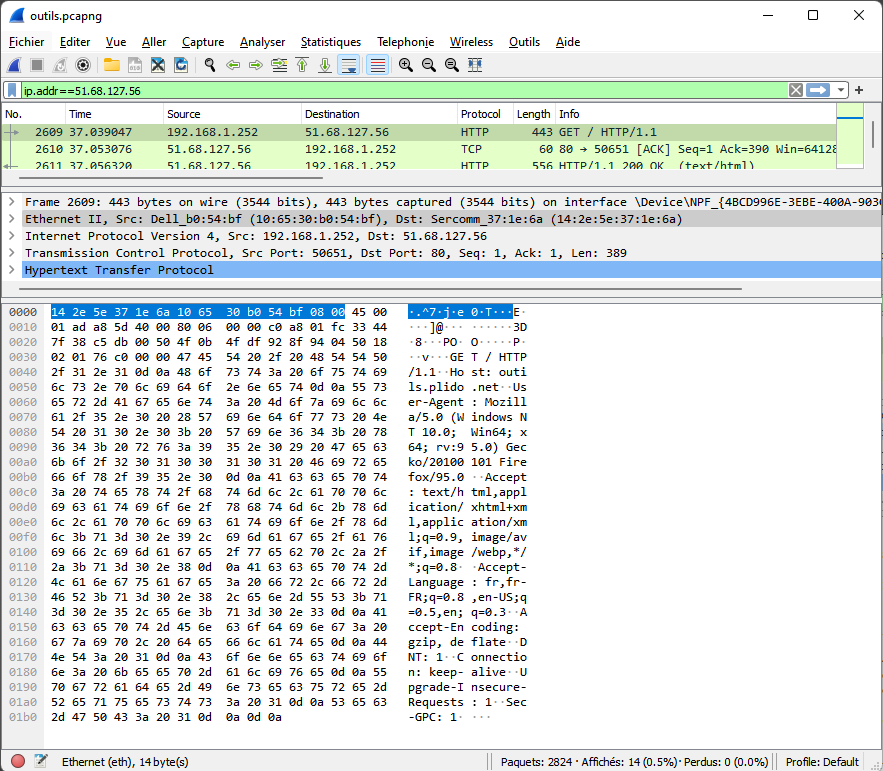
\includegraphics[width=1\columnwidth]{Pictures/ws-GET.png}}
\caption{Contenu de la trame transportant la requête HTTP GET}
\label{fig-ws-GET}
\end{figure}

  \vspace{1em}

La deuxième fenêtre montre la pile protocolaire, inversée par rapport aux représentations classique (cf. figure~\vref{fig-fullstack}), mais correspondant à l'ordre des encapsulations dans la trame. Comment Wireshark a pu arriver à un tel résultat.

\subsubsection{Ethernet}

Wireshark reçoit une trame du réseau \Index{Ethernet} ou \Index{Wi-Fi}\footnote{Pour le réseau Wi-Fi, il transforme le format en celui d'une trame Ethernet pour un affichage plus compact.}. Le format d'un trame Ethernet est défini par le standard \Index{IEEE 802.3}. L'en-tête contient trois champs~: 
\begin{itemize}
    \item 6 octets pour l'adresse MAC du destinataire,
    \item 6 octets pour l'adresse de la source.
    \item 2 octets pour le protocole de niveau supérieur. Ainsi la valeur \texttt{0x0800} désigne IPv4 et \texttt{0x86dd} IPv6.
\end{itemize}

  \vspace{1em}

Suivant le principe du modèle de référence de l'ISO, les adresses sont celles des nœuds adjacents, c'est-à-dire connecté au même réseau Ethernet ou Wi-Fi.

  \vspace{1em}

Dans notre cas, le protocole de niveau supérieur est donc un paquet IPv4 et Wireshark peut continuer à analyser, ce qui suit. Formellement se sont des données de la trame Ethernet, mais elles peuvent être comprise comme un paquet IPv4.

\Question{Mon adresse}{
Dasn l'exemple, figure~\vref{fig-ws-GET}, qu'elle est l'adresse Ethernet de la machine émettrice de la trame ?
}{
\texttt{10:65:30:b0:54:bf}. Attention, la trame commence par l'adresse de la destination, suivie de l'adresse de la source.
}

\subsubsection{IPv4}

Le format des paquets IPv4 défini dans le \rfc{791} a très peu évolué depuis sa publication en 1981. La figure~\vref{fig-header-IPv4} reprend ce format. Sans entrer dans les détails, les champs~:

\begin{itemize}
    \item adresse \texttt{source} et \texttt{destination} vont contenir les adresses IPv4 sur 32 bits des équipements d'extrémité. Des équipements intermédiaires, appelés routeur se chargent de recopier le paquet vers sa destination.
    \item Le champ \texttt{protocole} désigne la couche supérieure, la valeur 6 correspond à \Index{TCP} et 17 à \Index{UDP}.
\end{itemize}

\begin{figure}[tbp]

	\center {
    \begin{tikzpicture}

	\draw (0.5, 5.5) node  [right] {\tiny{\tt{0..................7...................15...................23....................31}}};
	
	 \draw (0.5, 5) node (context) [right, shade,  draw, minimum height=0.5cm, minimum width=1.2cm] {\tiny{Ver.}};

	\draw (1.7, 5) node (context) [right, draw, shade, minimum height=0.5cm, minimum width=1.2cm] {\tiny{IHL}};

	 \draw (2.9, 5) node (context) [right, draw, shade,  minimum height=0.5cm, minimum width=2.4cm] {\tiny{DiffServ}};

	 \draw (5.3, 5) node (context) [right, draw, shade,  minimum height=0.5cm, minimum width=4.8cm] {\tiny{Packet Length}};

	 \draw (0.5, 4.5) node (context) [right, draw, shade,  minimum height=0.5cm, minimum width=4.8cm] {\tiny{Identifier}};
	 \draw (5.3, 4.5) node (context) [right, draw, shade,  minimum height=0.5cm, minimum width=.9cm] {\tiny{flag}};
	 \draw (6.2, 4.5) node (context) [right, draw, shade,  minimum height=0.5cm, minimum width=3.9cm] {\tiny{Offset}};

	 \draw (2.9, 4) node (context) [right, draw, shade,  minimum height=0.5cm, minimum width=2.4cm, blue] {\tiny{Protocol}};

	 \draw (0.5, 4) node (context) [right, draw, shade,  minimum height=0.5cm, minimum width=2.4cm] {\tiny{TTL}};

	 \draw (5.3, 4) node (context) [right, draw, shade,  minimum height=0.5cm, minimum width=4.8cm] {\tiny{Checksum}};
	 
	 \draw (0.5, 3.5) node (context) [right, draw, shade,  minimum height=0.5cm, minimum width=9.6cm, blue] {\tiny{Source Address}};
	 \draw (0.5, 3) node (context) [right, draw, shade,  minimum height=0.5cm, minimum width=9.6cm, blue] {\tiny{Destination Address}};


	\end{tikzpicture}
	} %\center

\caption{Format d'un en-tête IPv4}
\label{fig-header-IPv4}
\end{figure}

\Question{saut par saut}{
Est-ce que l'adressse Ethernet \texttt{14:2e:5e:37:1e:6a} que l'on retrouve dans le paquet~\vref{fig-ws-GET} correspond à l'adresse Ethernet du destinataire du paquet ? A quoi correspond elle?
}{
Non, l'adresse Ethernet n'est valable que sur ce réseau Ethernet. Pour atteindre le destinataire le paquet devra traverser plusieurs routeurs. Comme la trame a été capturée sur la machine émettrice, cette adresse est donc celle du premier routeur traversé.
}

\subsubsection{TCP}

Wireshark, à partir du champ protocole valant 0x06, détermine que les données IP qui suivent l'en-tête sont un message TCP, il peut donc poursuivre le désassemblage de la trame. Le format de l'en-tête TCP est donné figure~\vref{fig-header-TCP}. Les numéros de port déterminent quelle application est utilisée. Si un client va prendre un numéro quelconque (50651 dans la trace figure~\vref{fig-ws-GET}), les serveurs vont utiliser des numéros connus de tous. Ainsi, les serveur Web se vont vus attribuer la valeur 80. Ils peuvent en choisir d'autres, comme on l'a vu lors de la constructions des \ac{URL}. 


\begin{figure}[tbp]

	\center {
    \begin{tikzpicture}

	\draw (0.5, 5.5) node  [right] {\tiny{\tt{0..................7...................15...................23....................31}}};
	
	 \draw (0.5, 5) node (SP) [right, shade,  draw, minimum height=0.5cm, minimum width=4.8cm] {};
	 \draw (SP) node [blue] {\tiny{Source Port}};

	 \draw (5.3, 5) node (DP) [right, shade,  draw, minimum height=0.5cm, minimum width=4.8cm] {};
	 \draw (DP) node [blue] {\tiny{Destination Port}};
	 
	 \draw (0.5, 4.5) node (seq) [right, shade,  draw, minimum height=0.5cm, minimum width=9.6cm] {};
	 \draw (seq) node  {\tiny{Sequence}};	 

	 \draw (0.5, 4) node (ack) [right, shade,  draw, minimum height=0.5cm, minimum width=9.6cm] {};
	 \draw (ack) node  {\tiny{Acknowledgment}};	 

	 \draw (0.5, 3.5) node (offset) [right, shade,  draw, minimum height=0.5cm, minimum width=1.2cm] {};
	 \draw (offset) node  {\tiny{Offset}};	 
	 
	 \draw (1.7, 3.5) node (res) [right, shade,  draw, minimum height=0.5cm, minimum width=1.8cm] {};
	 \draw (res) node  {\tiny{reserved}};	 
	 
	 \draw (5.3, 3.5) node (fin) [left, shade,  draw, minimum height=0.5cm, minimum width=0.3cm] {};
	 \draw (fin) node [rotate=90] {\tiny{FIN}};	 
	 \draw (5, 3.5) node (syn) [left, shade,  draw, minimum height=0.5cm, minimum width=0.3cm] {};
	 \draw (syn) node [rotate=90] {\tiny{SYN}};	 	 
	 \draw (4.7, 3.5) node (rst) [left, shade,  draw, minimum height=0.5cm, minimum width=0.3cm] {};
	 \draw (rst) node [rotate=90] {\tiny{RST}};	 	 
	 \draw (4.4, 3.5) node (psh) [left, shade,  draw, minimum height=0.5cm, minimum width=0.3cm] {};
	 \draw (psh) node [rotate=90] {\tiny{PSH}};	
	 \draw (4.1, 3.5) node (ack) [left, shade,  draw, minimum height=0.5cm, minimum width=0.3cm] {};
	 \draw (ack) node [rotate=90] {\tiny{ACK}};	
	 \draw (3.8, 3.5) node (urg) [left, shade,  draw, minimum height=0.5cm, minimum width=0.3cm] {};
	 \draw (urg) node [rotate=90] {\tiny{URG}};	
	 
	 \draw (5.3, 3.5) node (win) [right, shade,  draw, minimum height=0.5cm, minimum width=4.8cm] {};
	 \draw (win) node  {\tiny{Window}};	 	 
	 
	 \draw (0.5, 3) node (checksum) [right, shade,  draw, minimum height=0.5cm, minimum width=4.8cm] {};
	 \draw (checksum) node  {\tiny{Checksum}};

	 \draw (5.3, 3) node (urgent) [right, shade,  draw, minimum height=0.5cm, minimum width=4.8cm] {};
	 \draw (urgent) node  {\tiny{Urgent pointer}};

	 \draw (0.5, 2.5) node (option) [right,  draw, minimum height=1.5cm, minimum width=9.6cm] {};
	 \draw (option) node  {\tiny{Options}};	 	 
	 

	\end{tikzpicture}
	} %\center

\caption{Format d'un en-tête TCP}
\label{fig-header-TCP}
\end{figure}


Wireshark connaît cette liste de numéro de port bien connu et peut continuer à analyser la trame comme étant du HTTP.

Sans entrer dans les détails, on peut aussi remarquer une série de valeurs binaires qui servent par exemple à ouvrir ou fermer une connexion TCP. Si l'on reprend la phase d'ouverture de la connexion (cf. figure~\vref{fig-ws-filtre}), l'ouverture de connexion se fait par~:
\begin{itemize}
    \item l'émission par le client d'un message TCP avec le bit SYN de positionné,
    \item le serveur répond en positionnant les bits SYN et ACK dans son message,
    \item le client répond en renvoyant un message avec le bit ACK de positionné.
\end{itemize}

Ces trois messages qui ne contiennent pas de données servent à synchroniser la valeur initiale du champ \texttt{sequence} à chaque bout de la connexion.
  
\Question{Fermeture de connexion}{
A l'aide de la figure~\vref{fig-ws-GET} ou de vos captures Wireshark, quels sont les messages impliqués dans la fermeture du connexion?}
{La fermeture de déconnexion nécessite l'envoie de quatre message. L'une des extrémité, par forcement celle qui a ouvert la connexion, envoie un message avec le bit FIN positionné. Il est acquitté par l'autre entité qui a son tour envoie un message avec le bit FIN positionné qui sera acquitté pour définitivement fermer la connexion.
}   

\section{Do it yourself}\label{chap-flask}

Un serveur Web peut s'écrire en Python grâce au module \Index{Flask}. Le programme \texttt{simple\_server.py} permet de créer un serveur Web sur son ordinateur.

 \pythonlst{simple\_server.py}
 
 Ce script nécessite quelques explications :

\begin{itemize}
    \item Limport ligne 1 importe l'objet Flask à partir du module flask.
    \item A la ligne 2 une instance d'un objet Flask, c'est-à-dire un serveur web, est créée. Un nom lui est associé à des fins de débogage.
    \item A la ligne 4 contient la partie la plus délicate du script. \texttt{@} est un décorateur qui est utilisé en python pour ajouter des propriétés à une fonction. Ici, nous associons un chemin d'URI et une méthode REST à la fonction qui est ensuite définie. De cette façon, lorsque le serveur Flash recevra une requête GET sur ce chemin d'URI, il appellera la fonction \texttt{hello\_word}.
    \item La fonction texttt{hello\_word} retourne simplement un texte que le navigateur affichera.
    \item le serveur est lancé, ligne 8, en appelant la methode \pfunction{Flask}{run}. Il va attendre sur toutes les interfaces (adresse joker \texttt{0.0.0.0}) et sur le port 8080. 
\end{itemize}

  \vspace{1em}

Pour lancer le serveur, vous devez d'abord installer le module \texttt{Flask} avec \texttt{\Index{pip}}.

\begin{termc}[backgroundcolor=\color{palerod}, language=json, basicstyle=\ttfamily\small, escapechar=@]
# @\textbf{pip3 install Flask}@
Collecting Flask
  Downloading Flask-2.0.2-py3-none-any.whl (95 kB)
     |                                  | 95 kB 4.3 MB/s 
Collecting Jinja2>=3.0
  Downloading Jinja2-3.0.3-py3-none-any.whl (133 kB)
...
\end{termc}

  \vspace{1em}

Une fois le paquetage installé, il suffit d'exécuter le programme:
\begin{termc}[backgroundcolor=\color{palerod}, language=json, basicstyle=\ttfamily\small, escapechar=@]
# @\textbf{python3.9 simple\_server.py}@
 * Serving Flask app 'My First Web Server' (lazy loading)
 * Environment: production
   WARNING: This is a development server. Do not use it in a production
   deployment.
   Use a production WSGI server instead.
 * Debug mode: off
 * Running on all addresses.
   WARNING: This is a development server. Do not use it in a production
   deployment.
 * Running on http://192.168.1.53:8080/ (Press CTRL+C to quit)
127.0.0.1 - - [14/Dec/2021 21:06:55] "GET / HTTP/1.1" 200 -
127.0.0.1 - - [14/Dec/2021 21:06:59] "GET /favicon.ico HTTP/1.1" 404 -
\end{termc}


\Question{loopback}
{Quelle URI devez vous entrer dans votre navigateur pour accéder en local à ce serveur.}
{L'adresse de loopback est \texttt{127.0.0.1} et le port est 8080, le chemin d'URI est \texttt{/}. L'URI est donc \texttt{http://127.0.0.1:8080/}.}

\Question{Nom du serveur}{
A l'aide de Wireshark, pouvez vous déterminer dans la réponse les valeurs des options HTTP \texttt{\Index{Content-Type}} et \texttt{Server}.

Ne pas oublier que le trafic passe par l'interface \textit{loopback}. Pour afficher le trafic sur un port particulier, vous pouvez utiliser le filtre \texttt{tcp.port==XXXX}.
}{
On trouve les valeurs suivantes~:
\begin{itemize}
    \item \texttt{Server: Werkzeug/2.0.2 Python/3.9.6}
    \item \texttt{Content-Type: text/html; charset=utf-8}. La ressource est codée en HTML en utilisant un codage ASCII sur 8 bits.
\end{itemize}
}


%%%%%%%%%%%%%%%%%%%%%%%%%%%%%%%%%%%%%%%%%%%%%%%

% ModBus

%%%%%%%%%%%%%%%%%%%%%%%%%%%%%%%%%%%%%%%%%%%%%%%

\chapterimage{pano-tv1.png} % Chapter heading image

\chapter{Modbus}

\section{Introduction}
  \begin{wrapfigure}{r}{3cm}
\Youtube{https://youtu.be/Jj9Tmci7gXU}
\end{wrapfigure}
 \Index{Modbus} est apparu en 1979 à une époque où l'internet n'existait pas encore ! Il est toujours très populaire dans l'industrie. A l'origine Modbus était construit sur un bus série \Index{RS-485} qui connectait différents équipements  appelé (cf. figure~\vref{fig-modbus1})~:
 \begin{itemize}
 \item secondaires ou slaves et 
 \item un primaire appelée aussi master qui gère les communications. 
 \end{itemize}
 
 
 
 \begin{figure}[tbp]
\centerline{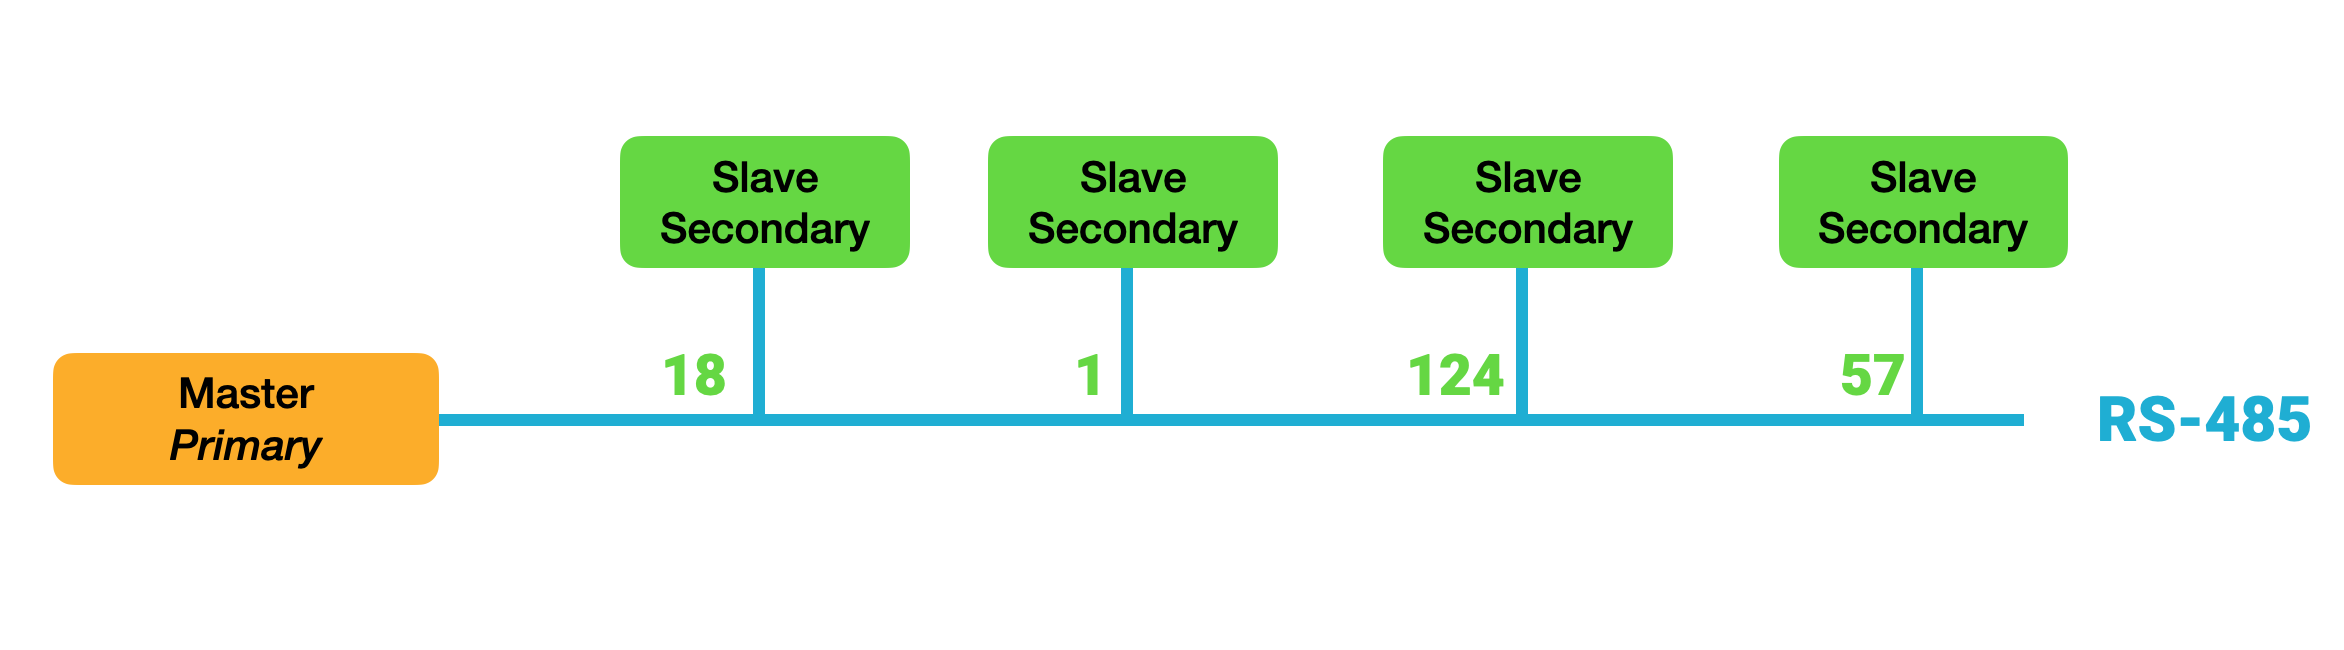
\includegraphics[width=1\columnwidth]{Pictures/Capture35.png}}
\caption{Architecture filaire de Modbus}
\label{fig-modbus1}
\end{figure}

 
 
 Chaque secondaire à un numéro unique ou adresse. Les adresses sont comprises entre 1 et 247. Le primaire n'a pas besoin d'une adresse puisque toutes les communications ont lieu avec lui. 
 
   \vspace{1em}


 Le primaire envoie une requête à un secondaire et le secondaire répond au primaire. Les communications directes entre deux secondaires ne sont pas possibles. 
 
 \subsection{Registres}
 
 
 Un équipement de Modbus peut prendre deux choses à travers des registres : 
 \begin{itemize}
     \item les relais qui peuvent prendre une valeur binaire "on" ou "off". Si le primaire peut modifier l'état et, bien sûr le lire, c'est appeler un \textit{\Index{coil}}. Si la valeur binaire peut uniquement être lu c'est un \textit{\Index{discrete input}}.
     \item des registres sur 16 bits. Ils sont utilisés pour représenter une valeur comme un courant électrique, une température, une vitesse de rotation,... De même, si on peut uniquement lire la valeur à est appelée un \textit{\Index{input register}} sinon, si elle peut être également être modifiée par le primaire, elle est appelée un \textit{\Index{holding register}}.
 \end{itemize}
 
    \vspace{1em}

 
Un équipement Modbus peut avoir jusqu'à 10~000 registres de ces quatre catégories. 

\subsection{Protocole}

Modbus est un protocole requête/réponse. Le primaire envoie une requête à l'adresse d'un équipement pour lire ou écrire un de ces registres. 
\begin{figure}[tbp]
\centerline{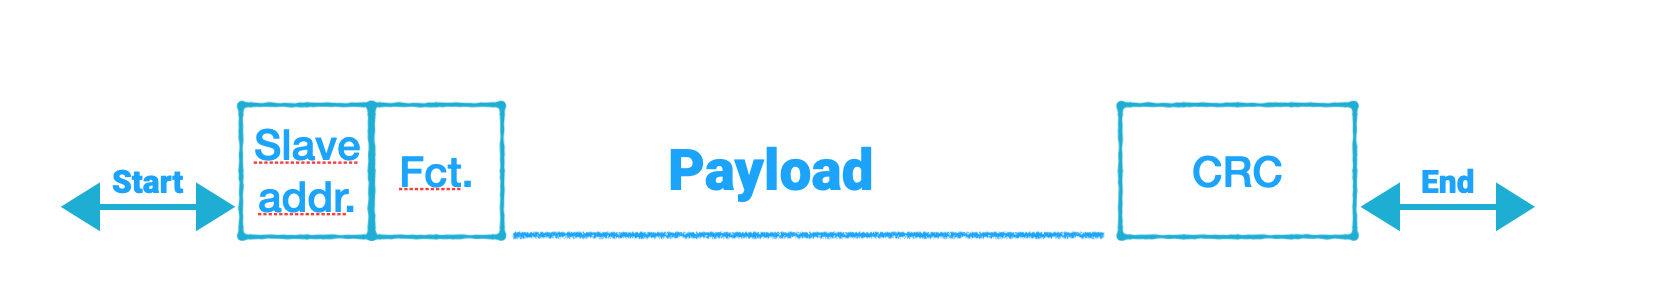
\includegraphics[width=1\columnwidth]{Pictures/Capture37.png}}
\caption{Trame Modbus}
\label{fig-modbus2}
\end{figure}

 

Une trame Modbus est une séquence de caractères commençant par un octet avec l'adresse du secondaire suivi d'une commande ou code de fonctions spécifique à chaque catégorie de registre~:
\begin{itemize}
    \item 1 pour lire un coil,
    \item 2 pour lire un discrete input,
    \item 3 pour lire un holding register,
    \item 4 pour lire un input register,
    \item 5 pour écrire un coil,
    \item 6 pour écrire un holding register,
\end{itemize}

    \vspace{1em}

La suite de la trame contient les données puis un \ac{CRC} pour valider qu'il n'y a pas d'erreur de transmission dans la trame. La partie donnée peut être différente dans la requête et la réponse. Par exemple pour lire un holding register, la requête contient l'adresse du premier registre à lire et le nombre de registres à lire et la réponse contient le nombre de données transmises suivi de leurs valeurs. Pour écrire sur un registre, les données de la trame seront l'adresse du registre et les données à écrire.

\subsection{Exemple: XY-MD02}


Regardons de plus près un exemple concret. On va utiliser un capteur de température et d'humidité, le \Index{XY-MD02} (cf. figure~\vref{fig-XYMD02}) dont les spécifications sont facilement accessibles via une recherche sur Internet. 

\begin{figure}[tbp]
\centerline{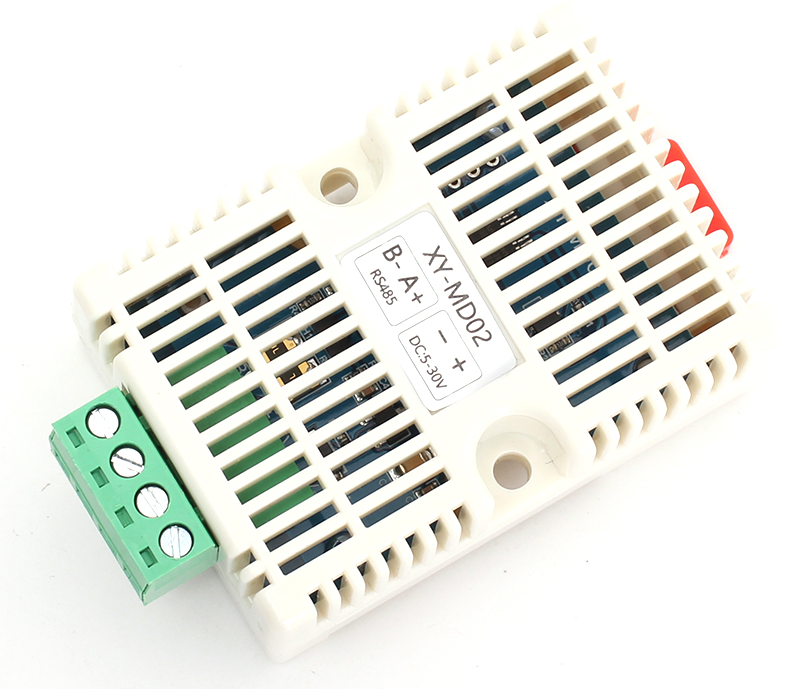
\includegraphics[width=0.6\columnwidth]{Pictures/XY-MD02.png}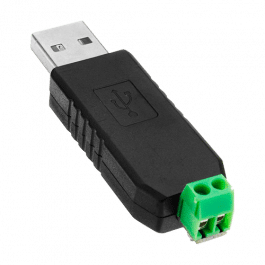
\includegraphics[width=0.4\columnwidth]{Pictures/rs485-usb.png}}
\caption{XY-MD02 et Adaptateur USB/RS-485}
\label{fig-XYMD02}
\end{figure}

La partie verte, se compose de quatre connecteurs dont la signification est indiquée sur l'étiquette. Les deux bornes de gauche constituent le bus \Index{RS-485} nommées \texttt{A+} et \texttt{B-} et les deux bornes de droites permettent d'alimenter électriquement l'équipement avec une tension comprise entre 5V et 30V.

    \vspace{1em}

 \begin{wrapfigure}{r}{3cm}
\Youtube{https://youtu.be/mnRiYaYt2uI}
\end{wrapfigure}

Un adaptateur \Index{USB}/\Index{RS-485} (cf. figure~\vref{fig-XYMD02}) est connecté à un ordinateur. On y retrouve les deux bornes A+ et B- du bus RS-846. L'ordinateur joue le rôle de primaire qui va interroger le capteur de température.  


    \vspace{1em}

Le programme \Index{QModMaster}\footnote{\url{https://sourceforge.net/projects/qmodmaster/}} (cf. figure~\vref{fig-qmodmaster}) permet d'interroger ou d'écrire les registres des secondaires. Dans la fenêtre de gauche permet d'accèder aux registres des secondaires. La fenêtre de droite montre le trafic ayant circulé sur le bus RS-485.

\begin{figure}[tbp]
\centerline{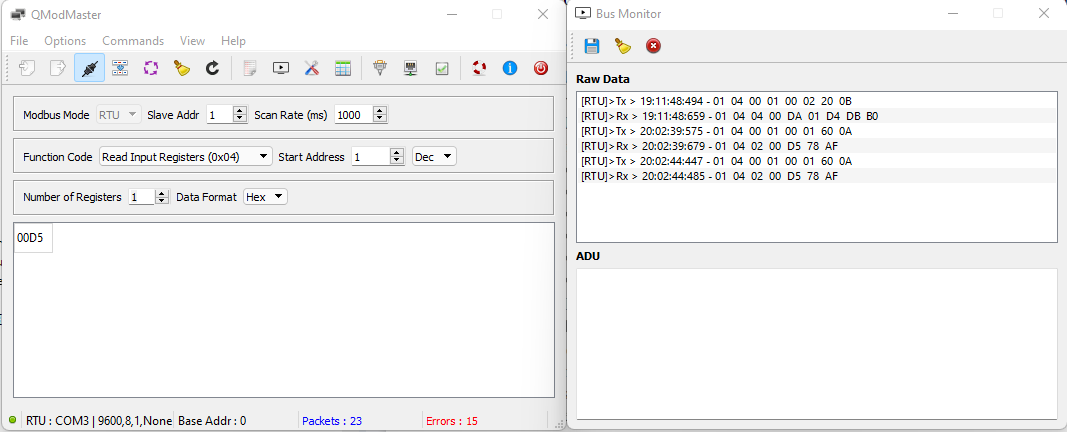
\includegraphics[width=1\columnwidth]{Pictures/modbus-trace.png}}
\caption{QModMaster avec trace des messages}
\label{fig-qmodmaster}
\end{figure}

Pour que le primaire puisse se connecter au secondaire, en plus du nom du port série (ici \texttt{COM3}), il faut disposer de plusieurs informations que l'on peut retrouver dans sa documentation :

\begin{itemize}
    \item la vitesse de transmission sur le bus (ici 9~600 bit/s) et le codage des caractères transmis (ici 8 bits sans bit de parité et un bit de stop)\footnote{\url{https://en.wikipedia.org/wiki/8-N-1}}.
    \item l'adresse du secondaire sur le bus.
\end{itemize}

    \vspace{1em}

La documentation donne également la nature des registres et leur codage. Le tableau~\vref{tab-XY-IR} reprend la définiton des \textit{Input Registers}. Il s'agit de registres qui ne peuvent qu'être lus. La spécification indique que la température est stockée dans le registre 1 sur une longueur de 2 octets, soit l'intégralité de celui-ci.

\begin{table}
\begin{center}
\begin{tabular}{|c|c|c|c|}
\hline
 \rowcolor{purple!10} Register Type & Register Address & Register Contents & Bytes \\ \hline \hline
 \multirow{2}{*}{Input register} & 0x0001 & Temperature & 2 \\ \cline{2-4}
                                 & 0x0002 & Humidity & 2 \\  \hline
\end{tabular}
\end{center}
\caption{Input Register d'un XY-MD02}
\label{tab-XY-IR}
\end{table}

    \vspace{1em}

La documentation indique que le secondaire a l'adresse 0x01 sur le bus RS-485. Il ne reste plus qu'à y envoyer une requête Modbus pour lire ce registre. La fenêtre de trace à droite sur la figure~\vref{fig-qmodmaster} donne les échanges. Nous allons analyser les deux dernières lignes. La première indique le contenu de la requête et la dernière la réponse du secondaire~:

\begin{termc}[backgroundcolor=\color{backcolour}, escapechar=@]
@\texttt{01 \textcolor{blue}{04} \textcolor{purple}{00 01} \textcolor{green!60!black}{00 01} \textcolor{black!30}{60 0A}}@
@\texttt{01 \textcolor{blue}{04} \textcolor{orange}{02} \textbf{00 D5} \textcolor{black!30}{78 AF}}@
\end{termc}

La requête commence par l'adresse du secondaire (\texttt{01}), puis par l'action (\texttt{\textcolor{blue}{04}}) pour lire un \textit{Input Register}, suivit de l'adresse du registre (\texttt{\textcolor{purple}{00 01}}) et du nombre de registres à lire (\textcolor{green!60!black}{00 01}). La requête se termine par la \ac{CRC} validant l'intégrité de la trame (\texttt{\textcolor{black!30}{60 0A}}).

la réponse contient également l'adresse du secondaire (\texttt{01}) et l'action, suivi de la taille de la réponse en octets (\texttt{\textcolor{orange}{02}}) et du résultat demandé (\texttt{\textbf{00 D5}}). 

\Question{Humidité}
{En regardant les échanges de la figure~\vref{fig-qmodmaster} quelle est la valeur mesurée pour l'humidité ?}
{Seul le premier échange demande la lecture de 2 registres à partir du registre ayant l'adresse 0x0001. Dans la réponse on obtient la valeur des deux registres consécutif (\texttt{00 DA} et \texttt{01 D4}). Le tableau~\vref{tab-XY-IR} indique que l'humidité est le second registre, on a donc \texttt{01 D4}.}

Reste à pouvoir interpréter cette valeur. La documentation indique que la valeur est en dixièmes de degrés et que l'unité est le Celsius. En convertissant \texttt{\textbf{00 D5}} en décimal, on obtient 213, soit 21.3\textcelsius.

\Question{Évolution des températures}
{En regardant les échanges de la figure~\vref{fig-qmodmaster} quelle est l'évolution de la température au cours du temps ?}
{On trouve 3 valeurs mesurées à 19:11:48, 20:02:39 et 20:02:44~: \texttt{00 DA}, \texttt{00 D5} et \texttt{00 D5}. Soit 21.8\textcelsius, 21.3\textcelsius ~~et 21.3\textcelsius.}

En résumé, on voit qu'il serait très difficile de faire fonctionner l'équipement sans documentation pour connaître : la vitesse du bus RS-485, l'adresse du secondaire, les adresses des registres utilisés et leur contenu et le codage de l'information dans les registres et les unités utilisées. On a donc un degrés d'interopérabilité faible, les deux entités doivent s'accorder sur un grand nombre de paramètres.

\Question{Taux d'Humidité}
{Quel est le taux d'humidité au moment de la mesure ? La documentation précise qu'il s'agit d'un pourcentage avec une précision au dizième de pourcent. }
{On avait lu la valeur \texttt{01 D4} dans le registre 0x02, soit 468 en décimal. D'où un taux d'humidité de 46.8\%}
    \vspace{1em}

On a pu communiquer avec l'objet en utilisant les paramètres par défaut. Mais pour l'insérer dans un bus, il faut pouvoir modifier certains paramètres. La vitesse de transmission et le codage des octets doit être le même, des secondaires ne peuvent pas avoir la même adresses sur le bus.
Le XY-MD02 dispose aussi de \textit{holding register} permettant de le paramétrage comme le montre la table~\vref{tab-XY-HR}


\begin{table}
\begin{center}
\begin{tabular}{|c|c|c|c|}
\hline
 \rowcolor{purple!10} Register Type & Register Address & Register Contents & Bytes \\ \hline \hline
 \multirow{9}{*}{Holding register} & 0x0101 & Device Address & 2 \\ \cline{2-4}
                                 & 0x1202 & Bit rate: & 2 \\
                                 &        & \tabitem 0~: 9600  & \\
                                 &        & \tabitem 1~: 14400 & \\
                                 &        & \tabitem 2~: 19200 & \\  \cline{2-4}
                                 & 0x0103 & Temperature correction & 2 \\ 
                                 &         & -10\textcelsius ~~- 10\textcelsius &  \\ \cline{2-4}
                                 & 0x0104 & Humidity correction & 2 \\ 
                                 &         & -10\%RH - 10\%RH &  \\ \hline
\end{tabular}
\end{center}
\caption{Holding Register d'un XY-MD02}
\label{tab-XY-HR}
\end{table}

\subsection{Passerelle IP}

\begin{wrapfigure}{r}{8cm}
\centerline{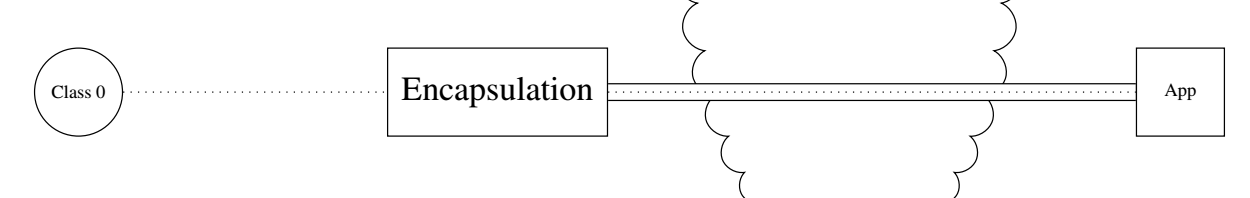
\includegraphics[width=.5\columnwidth]{Pictures/encaps3.png}}
\end{wrapfigure}

Il est possible d'étendre la portée d'un réseau Modbus en ajoutant une passerelle IP. Cela correspond au troisième méthode d'interconnexion de la figure~\vref{fig-encap}. La passerelle, connectée sur le bus où restent connectés les secondaires, possède une adresse IP. Le primaire ouvre une connexion TCP avec la passerelle et y envoie ses requêtes. La passerelle recopie les données sur le bus. Inversement, les réponses des objets sont retournées à la passerelle qui les envoie au primaire en utilisation la connexion TCP. La figure~\vref{fig-gwmodbus} illustre les échanges. On note l'ouverture de connexion TCP qui se fait au démarrage du primaire qui reste active pour toute les échanges. On peut aussi remarquer que les messages TCP sont acquittés. La figure~\vref{fig-msg-modbus} montre les champs commun aux format sur le bus RS-485 et dans des paquets IP.


\begin{figure}
    \centering
    
    \begin{tikzpicture}
    
    %\clip (0.0, 0) rectangle (16,10);
    %\draw[help lines] (0,0) grid (15,9); 
    
    \node[inner sep=0pt] (meter) at (1,7)
        {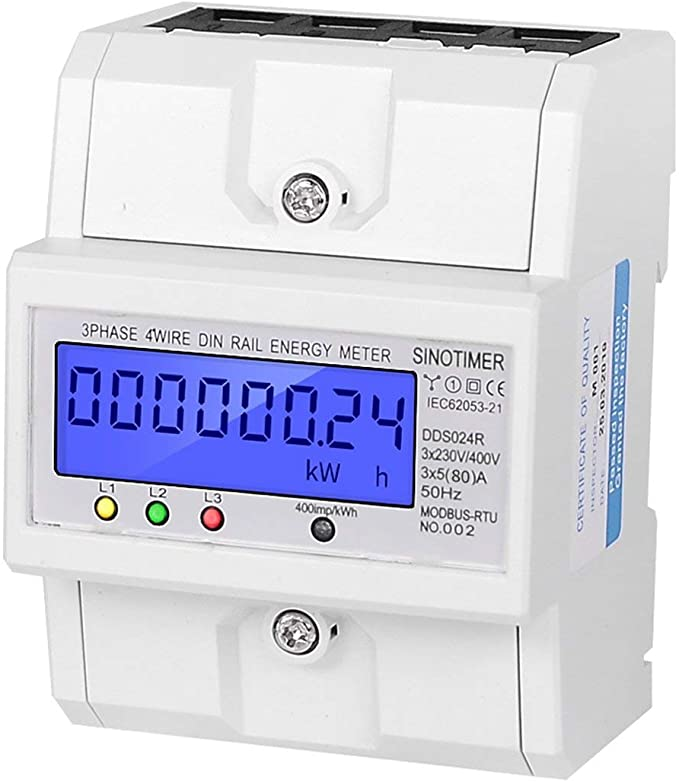
\includegraphics[width=.1\textwidth]{meter.jpg}};
        
    \node[inner sep=0pt] (gw) at (7,7)
        {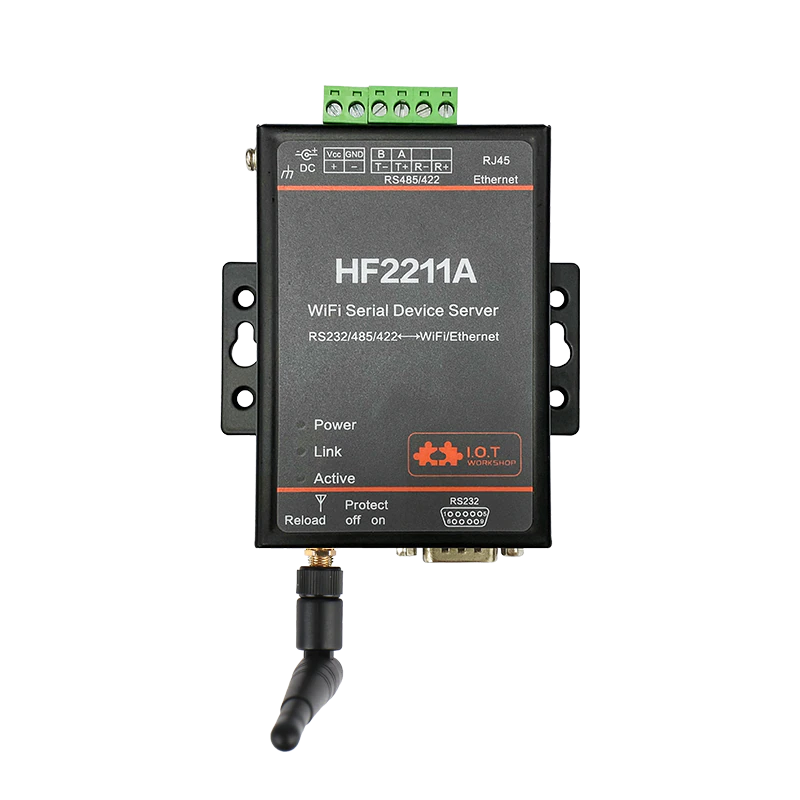
\includegraphics[width=.2\textwidth]{modbusGW2.png}};
    
    \node[inner sep=0pt] (primary) at (13,7)
        {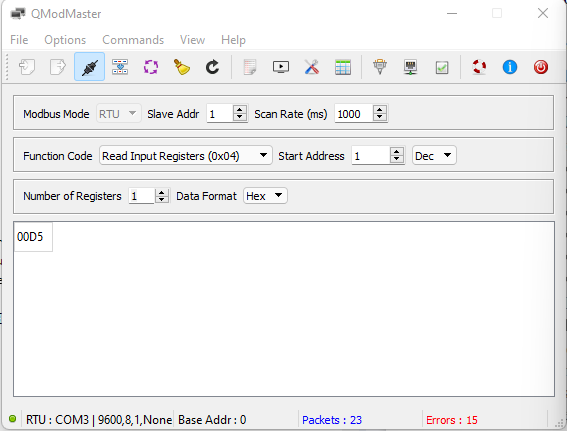
\includegraphics[width=.2\textwidth]{Pictures/QModMaster.png}};
        
        
    \coordinate (tline) at (0, 5.4);
    
    \draw (meter |- tline) node {\small{Compteur}};
    \draw (gw |- tline) node {\small{Passerelle}};
    \draw (primary |- tline) node {\small{Primaire}};
    
    \coordinate (wline) at (0, 8.3);
    
    \draw [decorate, decoration=snake, blue] (meter |- wline) -- coordinate(a)  (gw |- wline);
%    \draw [decorate, decoration={snake}, mirror, yellow] (gw |- wline) -- coordinate(a) (meter);
    
    \draw (a) node [below] {\small{RS-485}};
    
    \path(gw) -- coordinate(b) (primary);
    
    \draw [very thick] ([xshift=0.2cm]gw |- wline) -- coordinate(c) (primary |- wline);
     \draw (c) node [below] {\small{Internet}};
     
     \coordinate(cline) at (0, 5);
     
     \draw [->, thin] (meter |- cline) -- ++ (0, -4) ;
     \draw [->, thin] (gw |- cline) -- ++ (0, -4);
     \draw [->, thin] (primary |- cline) -- ++ (0, -4); 
     
     \draw [thick, ->] ([yshift=-0.1cm] primary |- cline) coordinate (d) -- ([yshift=-0.3cm] gw |- cline) coordinate (e);
     
     \draw (d) node [right] {\tiny{SYN}};
     \draw (e) node [left] {\tiny{SYN/ACK}};
     \draw [thick, ->] (e) -- ([yshift=-0.5cm] primary |- cline) coordinate (f);
     
    \draw (f) node [right] {\tiny{ACK}};
    \draw [thick, ->] (f) -- ([yshift=-0.7cm] gw |- cline) coordinate (h);
    
    \coordinate (tcp_line) at (14.5, 0);
    
    \draw [decoration=brace, decorate] (d -| tcp_line) -- coordinate(i) (h -| tcp_line);
    
    \draw (i) node [below, rotate=90] {\small{Ouverture}};
    
    \draw [double, double distance=0.2cm,] ([yshift=-1.5cm] primary |- cline) coordinate (d) -- ([yshift=-1.7cm] gw |- cline) coordinate (e);
    
    
    \draw  [->] ([yshift=-1.8cm] gw |- cline) -- ([yshift=-2cm] primary |- cline) coordinate(k);
    \draw (k) node [right] {\tiny{ACK}};


    \draw [purple, -> ] ([yshift=-1.5cm] primary |- cline) coordinate (d) -- ([yshift=-1.7cm] gw |- cline);      
    \draw [purple, -> ] ([yshift=-1.7cm] gw |- cline)  -- ([yshift=-2.1cm] meter |- cline) coordinate (e);  

    \draw (d) node [right,purple] {\small{requête}};

    \draw [blue, ] (e) -- ([yshift=-2.5cm] gw |- cline);    
    \draw [double, double distance=0.2cm ] ([yshift=-2.5cm] gw |- cline) -- ([yshift=-2.7cm] primary |- cline);    
    \draw [blue, -> ] ([yshift=-2.5cm] gw |- cline) -- ([yshift=-2.7cm] primary |- cline) coordinate(m);   
    
    \draw  [->] ([yshift=-2.8cm] primary |- cline) -- ([yshift=-3cm] gw |- cline) coordinate(l);
    \draw (l) node [left] {\tiny{ACK}};
    
    \draw (m) node [right,blue] {\small{réponse}};

   
    \end{tikzpicture}
    
    \caption{Passerelle entre le réseau Internet et Modbus.}
    
    \label{fig-gwmodbus}
\end{figure}

\begin{figure}
    \centering
    
    \begin{tikzpicture}
    
  
    
    
    
    \draw (0,0) node (tid) [rectangle, draw,  minimum width = 2cm, minimum height = 0.5cm, fill=olive!50 ] {};
    \draw (tid) node {\tiny{Transaction ID}};


    \draw (tid.east) node (pid) [right, rectangle, draw,  minimum width = 2cm, minimum height = 0.5cm, fill=olive!50 ] {};
    \draw (pid) node {\tiny{Protocol ID}};

    \draw (pid.east) node (len) [right, rectangle, draw,  minimum width = 2cm, minimum height = 0.5cm, fill=olive!50 ] {};
    \draw (len) node {\tiny{Length}};
    
    \draw (len.east) node (uid) [right, rectangle, draw,  minimum width = 1cm, minimum height = 0.5cm, fill=olive!50 ] {};
    \draw (uid) node {\tiny{Unit ID}};

    \draw (uid.east) node (fcode) [right, rectangle, draw,  minimum width = 1cm, minimum height = 0.5cm, fill=green!50 ] {};
    \draw (fcode) node {\tiny{FCode}};
    
    \draw (fcode.east) node (data) [right, rectangle, draw,  minimum width = 4cm, minimum height = 0.5cm, fill=green!50 ] {};
    \draw (data) node {\tiny{Data}};
    
    \draw [green!50] (data.north) -- +(-1, 0) -- +(1, 0);
    \draw [green!50] (data.south) -- +(-1, 0) -- +(1, 0);
    \draw [dashed] (data.north) -- +(-1, 0) -- +(1, 0);
    \draw [dashed] (data.south) -- +(-1, 0) -- +(1, 0);
    
    \draw (data.east) node [right] {\small{TCP}};
    
    
    \path (uid.west) -- ++(0, 1.5) coordinate(x);
    \draw (x) node (addr) [right, rectangle, draw,  minimum width = 1cm, minimum height = 0.5cm, fill=olive!50 ] {};
    \draw (addr) node {\tiny{Addr}};  

   \draw (addr.east) node (fcode) [right, rectangle, draw,  minimum width = 1cm, minimum height = 0.5cm, fill=green!50 ] {};
    \draw (fcode) node {\tiny{FCode}};
    
    \draw (fcode.east) node (data) [right, rectangle, draw,  minimum width = 4cm, minimum height = 0.5cm, fill=green!50 ] {};
    \draw (data) node {\tiny{Data}};    
   \draw [green!50] (data.north) -- +(-1, 0) -- +(1, 0);
    \draw [green!50] (data.south) -- +(-1, 0) -- +(1, 0);
    \draw [dashed] (data.north) -- +(-1, 0) -- +(1, 0);
    \draw [dashed] (data.south) -- +(-1, 0) -- +(1, 0);
    

    \draw (data.east) node (crc) [right, rectangle, draw,  minimum width = 2cm, minimum height = 0.5cm, fill=blue!50 ] {};
    \draw (crc) node {\tiny{CRC}};
    
    \draw(x) node [left] {\small{RS-385}};
    \end{tikzpicture}
    
    \caption{Messages Modbus sur bus RS-485 et sur IP/TCP}
    
    \label{fig-msg-modbus}
\end{figure}


Comme dans l'exemple précédent du capteur de température, les spécifications du \Index{compteur électrique} sont nécessaires pour comprendre la signification des registres utilisables. Le compteur code ses valeurs sur des nombres flottant sur 32 bits dont le codage est spécifié par la norme \Index{IEEE 754}\footnote{\url{https://en.wikipedia.org/wiki/IEEE_754}}. Ces valeurs sur 32 bits doivent être codées sur deux registres consécutifs d'où l'incrémentation de 2 en 2 que l'on retrouve sur la tableau~\vref{tab-meter-IR}, le compteur pouvant mesurer trois phase électriques.


\begin{table}
\begin{center}
\begin{tabular}{|c|c|c|c|c|}
\hline
 \rowcolor{purple!10} Register Type & Register Address & Register Contents & Unité & Format \\ \hline \hline
 \multirow{10}{*}{Input register} & 0x0000 & \Index{Voltage} phase A & V &  IEEE 754 \\ \cline{2-5}
                                 & 0x0002 & Voltage phase B & V &  IEEE 754 \\ \cline{2-5}
                                 & 0x0004 & Voltage phase C & V &  IEEE 754 \\ \cline{2-5}
                                 & 0x0008 & \Index{Intensité} phase A & A &  IEEE 754 \\ \cline{2-5}
                                 & 0x000A & Intensité phase B & A &  IEEE 754 \\ \cline{2-5}
                                 & 0x000C & Intensité phase C & A &  IEEE 754 \\ \cline{2-5}
                                 & 0x0010 & \Index{Puissance} Totale & KWh &  IEEE 754 \\ \cline{2-5}
                                 & 0x0012 & Puissance phase A & KWh &  IEEE 754 \\ \cline{2-5}
                                 & 0x0014 & Puissance phase B & KWh &  IEEE 754 \\ \cline{2-5}
                                 & 0x0016 & Puissance phase C & KWh &  IEEE 754 \\ \cline{2-5}
                                 & 0x0036 & \Index{Fréquence} & Hz &  IEEE 754 \\ \hline

\end{tabular}
\end{center}
\caption{quelques \textit{Input Register} du compteur électrique}
\label{tab-meter-IR}
\end{table}

    \vspace{1em}

\Index{Wireshark} peut capturer une requête ayant circulé sur le réseau Ethernet, coté primaire (cf. figure~\vref{fig-modbus-ws}).

\begin{figure}[tbp]
\centerline{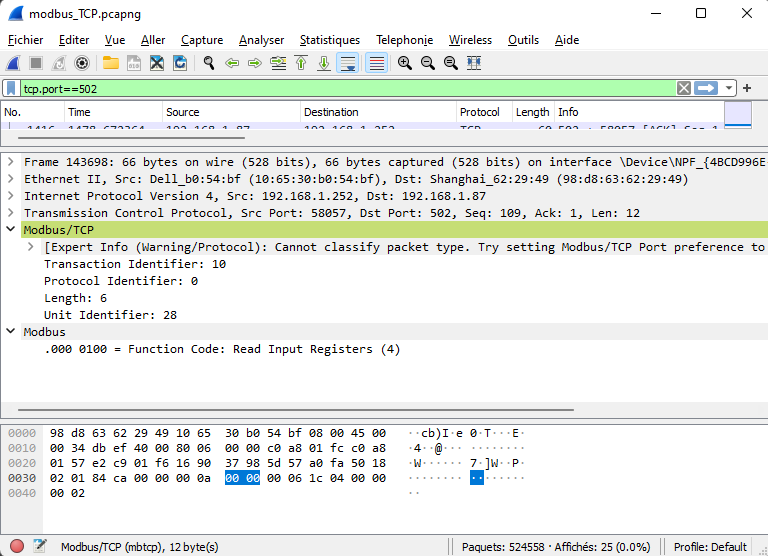
\includegraphics[width=1\columnwidth]{Pictures/modbus-ws.png}}
\caption{Capture avec \Index{Wireshark} d'une trame contenant un message Modbus.}
\label{fig-modbus-ws}
\end{figure}


\begin{termc}[backgroundcolor=\color{backcolour}, escapechar=#]
#\texttt{\small{0000 \colorbox{purple!50}{98 d8 63 62 29 49 10 65 30 b0 54 bf 08 00}\colorbox{blue!30}{45 00}   ..cb)I.e0.T...E.}}#
#\texttt{\small{0010  \colorbox{blue!30}{00 34 db ef 40 00 80 06 00 00 c0 a8 01 fc c0 a8}   .4..@...........}}#
#\texttt{\small{0020  \colorbox{blue!30}{01 57}\colorbox{red!30}{e2 c9 01 f6 16 90 37 98 5d 57 a0 fa 50 18}   .W......7.]W..P.}}#
#\texttt{\small{0030  \colorbox{red!30}{02 01 84 ca 00 00} \ul{00 0a} \ul{00 00} \ul{00 06} 1c \textcolor{blue}{04} \textcolor{red}{00 00}   ................}}#
#\texttt{\small{0040  \textcolor{green}{00 02}   ..              }}#                                 
\end{termc}

On retrouve les encapsulations des protocoles Ethernet, IP et TCP, suivi des données TCP. Elles se composent de  trois champs qui n'existent pas dans la requête circulant sur le bus RS-485~:
\begin{itemize}
    \item le numéro de la transaction sur deux octets incrémenté à chaque requête,
    \item la version du protocole sur deux octets, 
    \item la longueur en octet de la transaction.
\end{itemize}

    \vspace{1em}

Les champs suivants sont identiques à ceux de la trame sur le bus RS-485~:
\begin{itemize}
    \item l'adresse du secondaire sur un octet, ici 0x1c ou 28,
    \item la nature de la requête : 0x04 pour lire un \textit{input register},
    \item le registre à lire sur deux octets, ici 0x0000 correspondant à la tension sur la phase A.
    \item le nombre de registre à lire, ici 2 pour obtenir les 32 bits de la valeur.
\end{itemize}

    \vspace{1em}

Le primaire reçoit la réponse suivante~:

\begin{termc}[backgroundcolor=\color{backcolour}, escapechar=#]
#\texttt{\small{0000  \colorbox{purple!50}{10 65 30 b0 54 bf 98 d8 63 62 29 49 08 00}\colorbox{blue!30}{45 00}   .e0.T...cb)I..E.}}# 
#\texttt{\small{0010  \colorbox{blue!30}{00 35 c9 75 00 00 40 06 2c aa c0 a8 01 57 c0 a8}   .5.u..@.,....W..}}# 
#\texttt{\small{0020  \colorbox{blue!30}{01 fc}\colorbox{red!30}{01 f6 e2 c9 5d 57 a0 fa 16 90 37 a4 50 18}   ......]W....7.P.}}# 
#\texttt{\small{0030  \colorbox{red!30}{44 70 e1 6e 00 00} \ul{00 0a} \ul{00 00} \ul{00 07} 1c \textcolor{blue}{04} \textcolor{orange}{04}\colorbox{black}{\textcolor{white}{43}}   Dp.n...........C}}# 
#\texttt{\small{0040  \colorbox{black}{\textcolor{white}{69 9e 4a}} \ \ \ \ \ \ \ \ \ \ \ \ \ \ \ \ \ \ \ \ \ \ \ \ \ \ \ \ \ \ \ \ \ \ \ \ \ \ \ i.J}}# 
                           
\end{termc}

On y retrouve, après les encapsulations protocolaires d'Ethernet, IP et TCP les données suivantes~:
\begin{itemize}
    \item le numéro de transaction qui correspond à celui employé dans la requête précédente. cela permet de faire le lien entre les deux messages qui aurait pu se défaire en cas de perte de paquets sur le réseau Internet,
    \item la version du protocole,
    \item la longueur de la réponse, ici 7 octets,
    \item l'adresse du secondaire ayant répondu, ici 28,
    \item la nature de la requête,
    \item le nombre d'octets retournés, ici 4,
    \item et la valeur des deux registres \texttt{0x43699e4a} qui correspond à un nombre flottant tel que le représente le standard IEEE 754. Il existe de nombreux sites sur Internet qui permettent la conversion\footnote{\url{https://www.h-schmidt.net/FloatConverter/IEEE754.html}}. Comme le montre la figure~\vref{fig-ieee754}, on obtient la valeur \SI{233.61831665}\volt qui correspond bien à une tension offerte par un réseau électrique.
\end{itemize}

  \begin{figure}[tbp]
\centerline{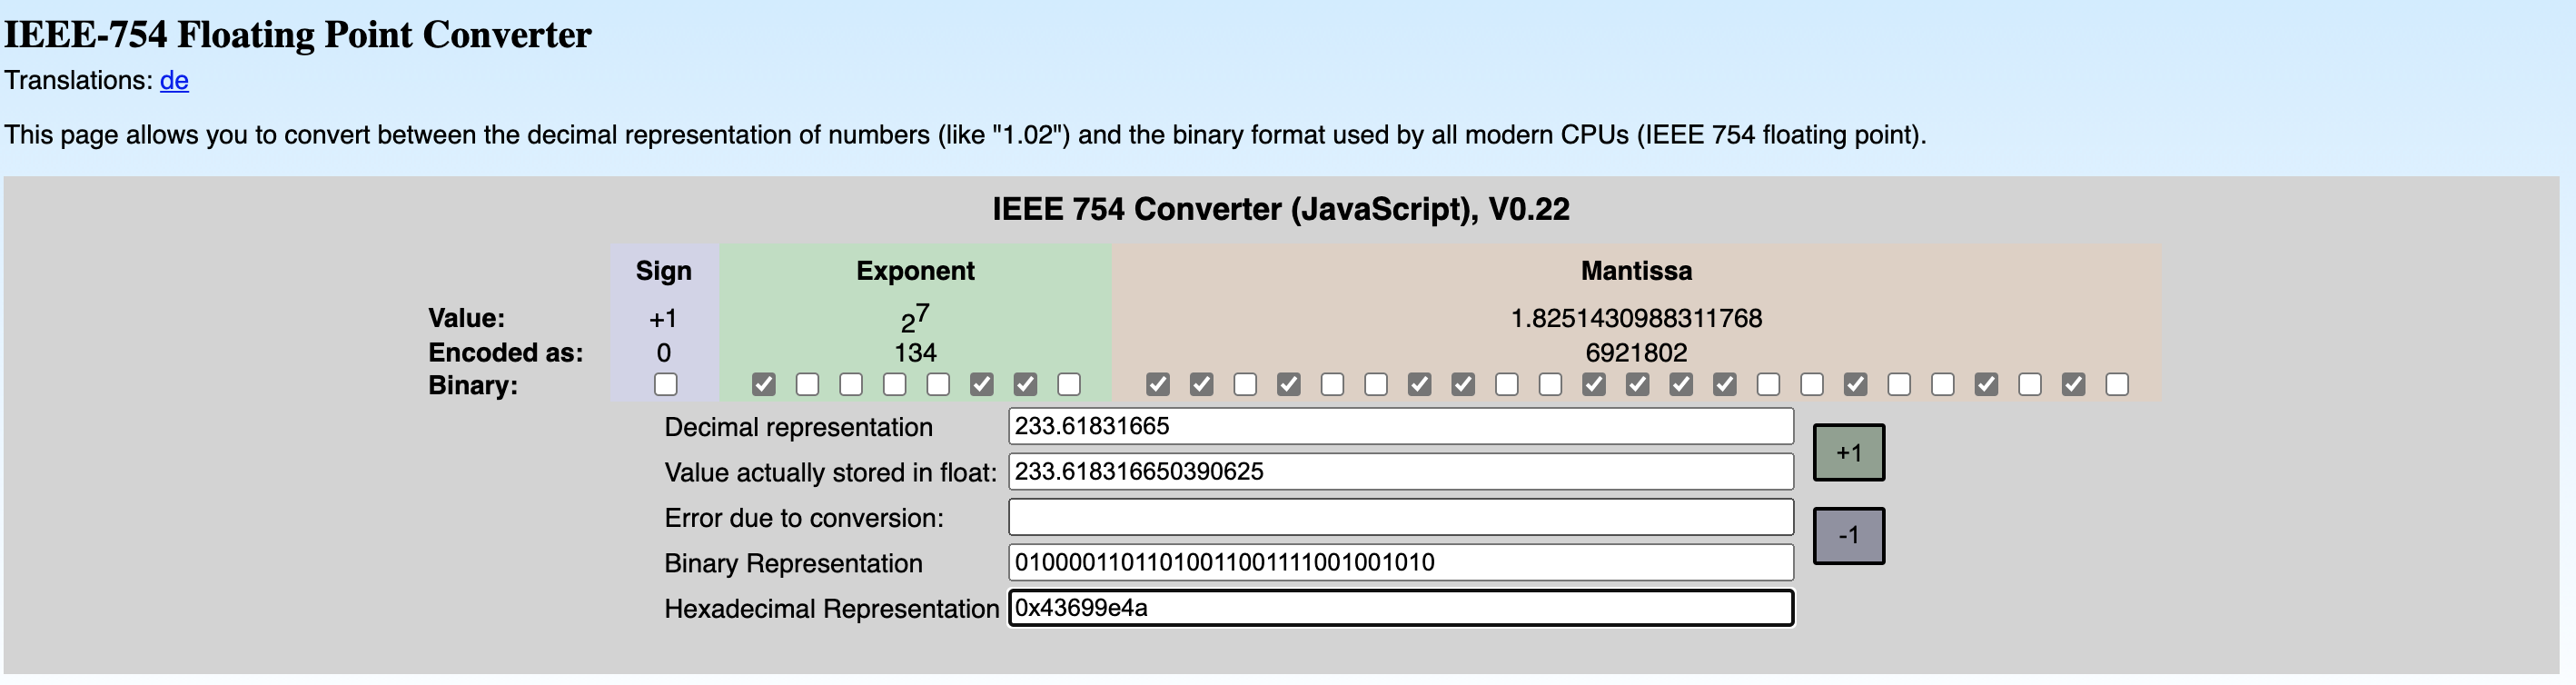
\includegraphics[width=1\columnwidth]{Pictures/IEEE754.png}}
\caption{Conversion d'un nombre flottant}
\label{fig-ieee754}
\end{figure}

\Question{Requête Modbus TCP}
{Soit l'échange donné figure~\vref{fig-exo-ws} correspondant à une requête Modbus et à une réponse.
Quel est le numéro de port utilisé par Modbus TCP.}
{Il y a deux ports dasn l'en-tête TCP, mais comme il s'agit d'une requête, il faut prendre le port destination~:0x1f6, soit 502 en décimal}

\Question{Requête Modbus TCP}
{En poursuivant l'analyse du trafic, quelle valeur de registre est demandée.}
{Le registre 0x36 est demandé, en regardant dans la table~\vref{tab-meter-IR}, il s'agit de la fréquence en Hz}

\Question{Réponse Modbus TCP}
{En analysant le paquet suivant, 
Comment peut-on vérifier que la réponse peut correspondre à la requête précédente.}
{Le numéro de séquence 0x000c est le même dans les deux trames.}


\Question{Réponse Modbus TCP}
{Quelle valeur est retournée. Est-ce cohérent ?}
{La valeur du registre est 0x4247e95b correspond à un nombre flottant IEEE 754, en convertissant on obtient la valeur 49.9778862 Hz qui est très proche de la fréquence du réseau électrique européen.}

\begin{figure}[tbp]

\begin{termc}[backgroundcolor=\color{backcolour}, escapechar=#]
#\texttt{\small{0000  \colorbox{purple!50}{98 d8 63 62 29 49 10 65 30 b0 54 bf 08 00}\colorbox{blue!30}{45 00}   ..cb)I.e0.T...E.}}#
#\texttt{\small{0010  \colorbox{blue!30}{00 34 db f3 40 00 80 06 00 00 c0 a8 01 fc c0 a8}   .4..@...........}}#
#\texttt{\small{0020  \colorbox{blue!30}{01 57}\colorbox{red!30}{e2 c9 01 f6 16 90 37 b0 5d 57 a1 14 50 18}   .W......7.]W..P.}}#
#\texttt{\small{0030  \colorbox{red!30}{02 01 84 ca 00 00} 00 0c 00 00 00 06 1c 04 00 36   ...............6}}#
#\texttt{\small{0040  00 02 \ \ \ \ \ \ \ \ \ \ \ \ \ \ \ \ \ \ \ \ \ \ \ \ \ \ \ \ \ \ \ \ \ \ \ \ \ \ \ \ \ \  ..}}#
                           
\end{termc}

\begin{termc}[backgroundcolor=\color{backcolour}, escapechar=#]
#\texttt{\small{0000  \colorbox{purple!50}{10 65 30 b0 54 bf 98 d8 63 62 29 49 08 00}\colorbox{blue!30}{45 00}   .e0.T...cb)I..E.}}#
#\texttt{\small{0010  \colorbox{blue!30}{00 35 8b 15 00 00 40 06 6b 0a c0 a8 01 57 c0 a8}   .5....@.k....W..}}#
#\texttt{\small{0020  \colorbox{blue!30}{01 fc}\colorbox{red!30}{01 f6 e2 c9 5d 57 a1 14 16 90 37 bc 50 18}   ......]W....7.P.}}#
#\texttt{\small{0030  \colorbox{red!30}{44 70 f1 f0 00 00} 00 0c 00 00 00 07 1c 04 04 42   Dp.............B}}#
#\texttt{\small{0040  47 e9 5b \ \ \ \ \ \ \ \ \ \ \ \ \ \ \ \ \ \ \ \ \ \ \ \ \ \ \ \ \ \ \ \ \ \ \ \ \ \ \ \  G.[}}#
                           
\end{termc}
\caption{Capture à étudier.}
\label{fig-exo-ws}
\end{figure}
\chapter{ARCHITECTURE POUR L'IOT}

\section{Introduction}
  
    \vspace{1em}
   
 \begin{wrapfigure}{r}{3cm}
\Youtube{https://youtu.be/DjRhnbg0FjY}
\end{wrapfigure}

Les objets se caractérisent 
par 
une capacité
de traitement limitée et par une consommation énergétique réduite pour préserver l’autonomie imposée par une alimentation sur batterie.
Or, les activités les plus consommatrices pour un équipement sont l’émission et la réception de données. 
Pour maximiser l’autonomie des équipements, il faut revoir l’intégralité des protocoles, mais en les calquant sur les architectures existantes pour en assurer la compatibilité. 

La figure~\vref{fig-pile-IoT} reprend un certain nombre d'adaptation protocolaires, à différents niveau du modèle \ac{ISO}, capable de s'adapter aux caractéristiques des objets contraints. Dans les chapitres suivants nous reviendrons sur ces technologies en partant de la représentation des données pour aller jusqu'aux couches basses.

\begin{figure}[tbp]
\centerline{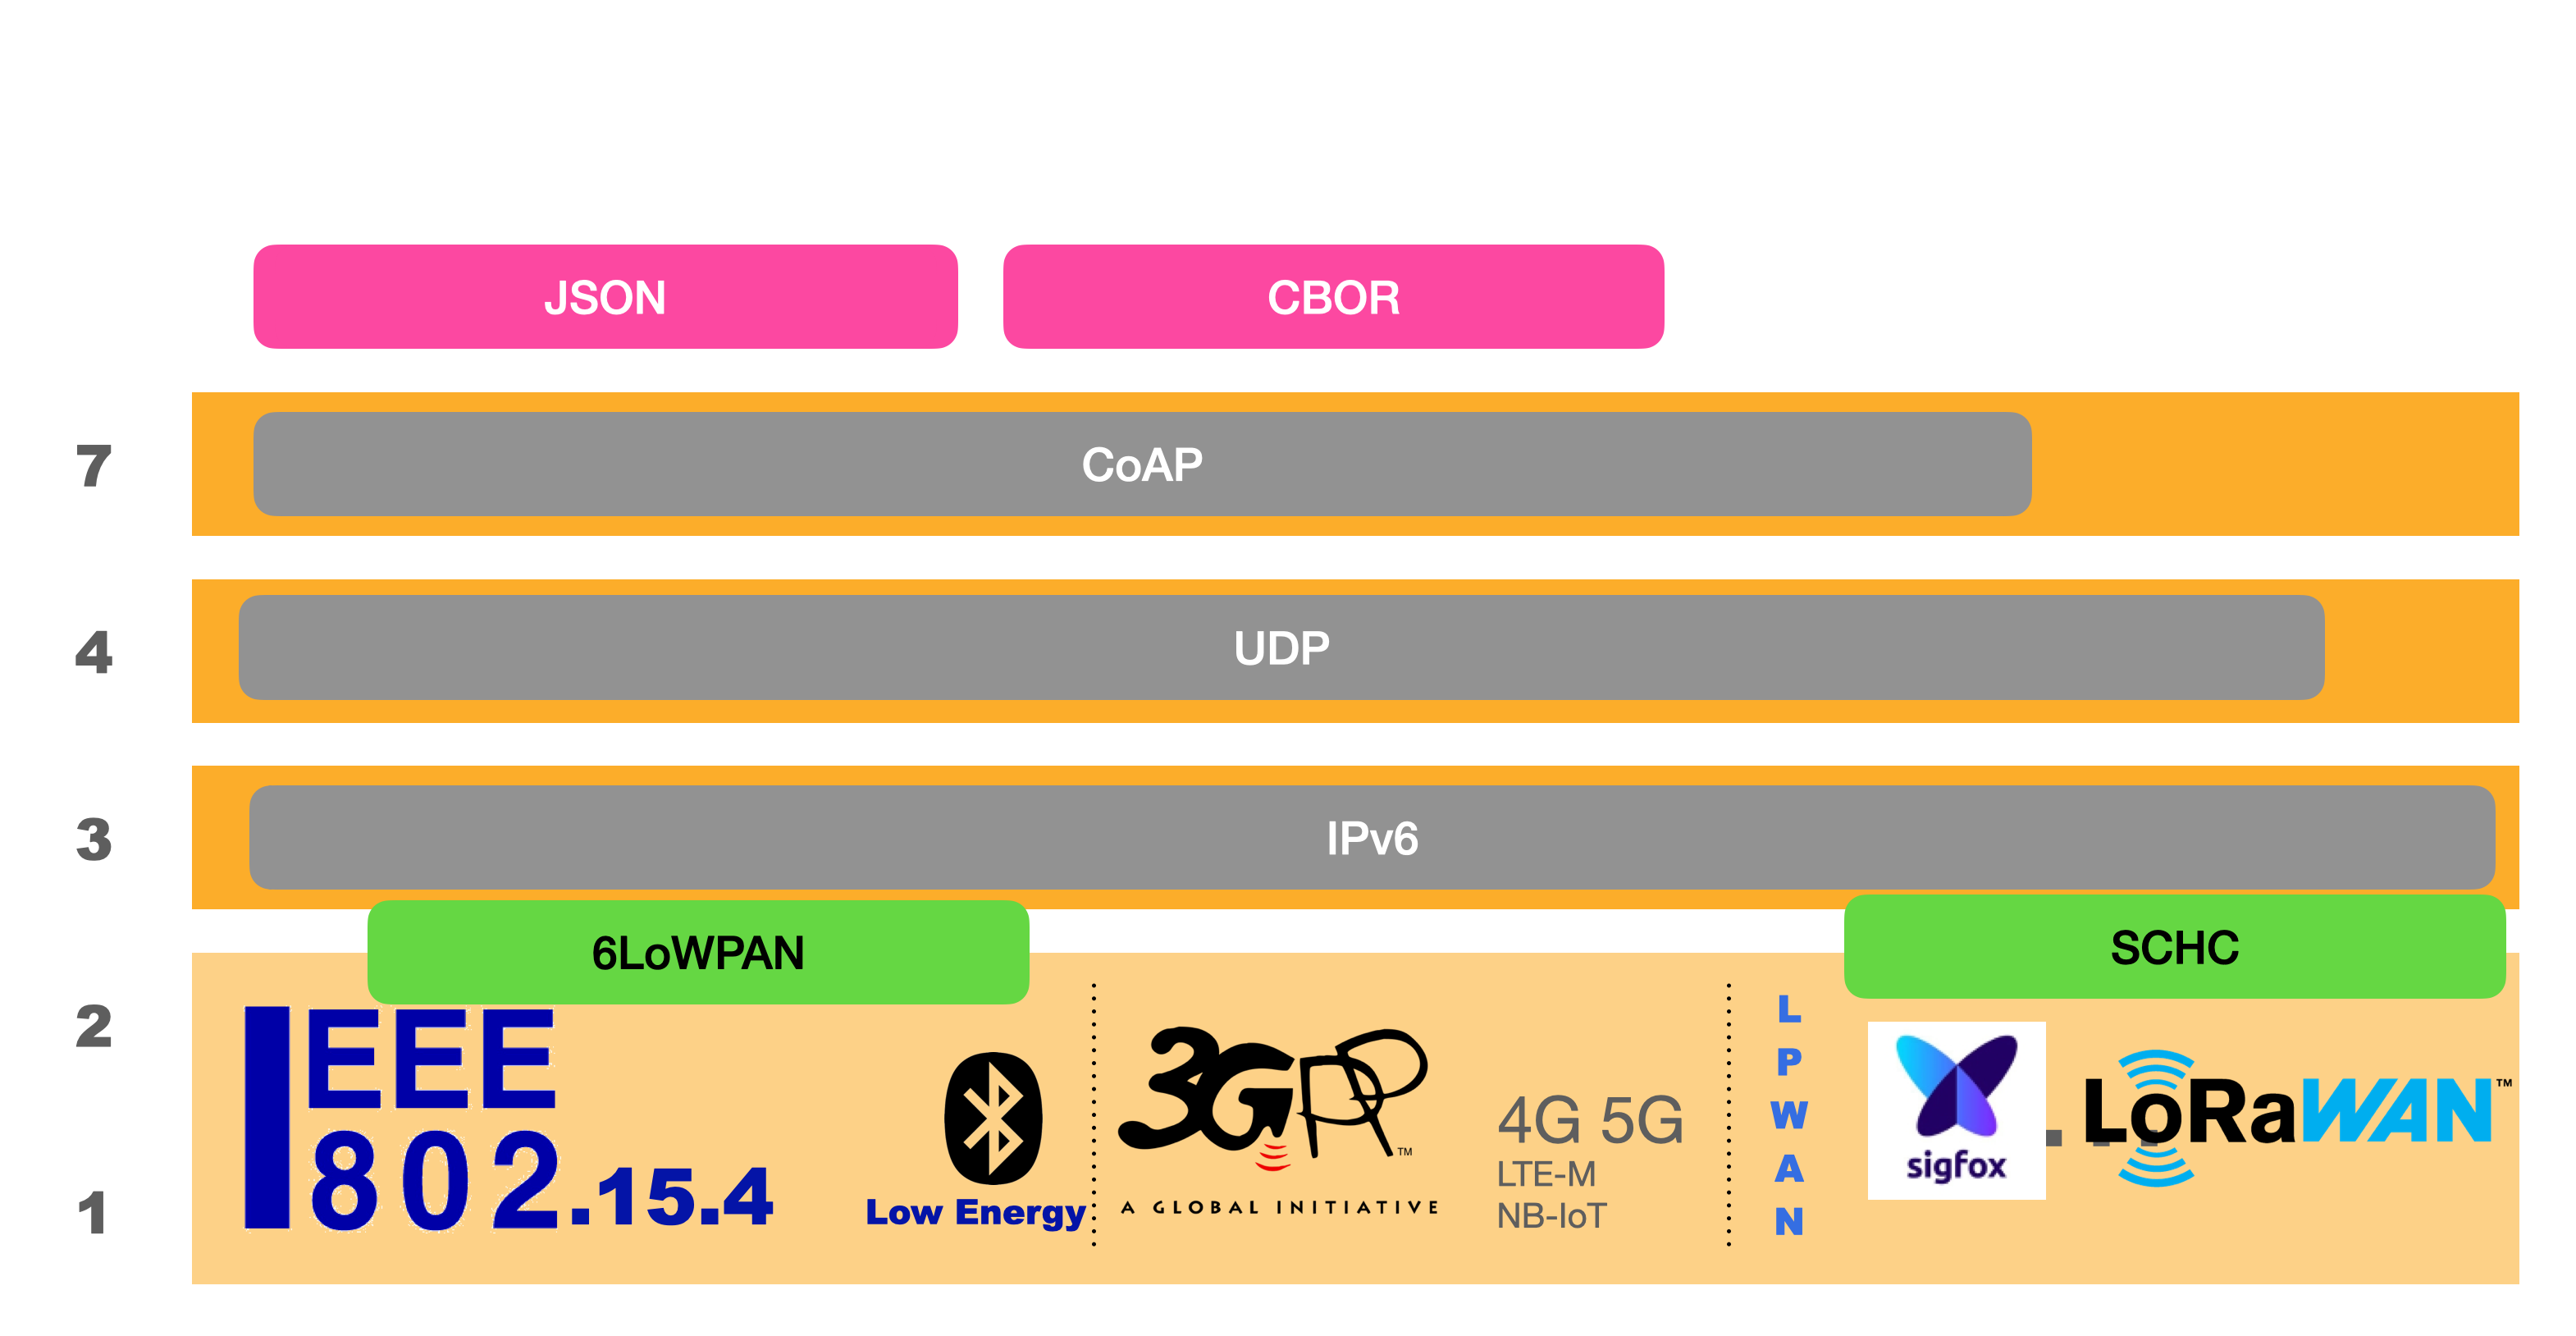
\includegraphics[width=1\columnwidth]{Pictures/Capture17.png}}
\caption{Pile protocolaire de l'IoT}
\label{fig-pile-IoT}
\end{figure}

\section{Topologies}

Les réseaux pour l’internet des objets peuvent être divisés en deux catégories : les topologies \Index{maillé}es (\Index{Mesh} in english) et étoilées (\Index{star}).


\subsection*{Réseaux Maillés}

Les réseaux maillés, tels que la famille IEEE 802.15.4,  sont une adaptation d’un protocole d’accès Wi-Fi pour préserver l’énergie. La portée de transmission est limitée à 50 mètres pour limiter la consommation d'énergie ; et par conséquent les messages doivent être relayés par d’autres nœuds pour atteindre leur destination.

Le débit est de quelques centaines de kilobits/s et la taille de la trame est de quelques centaines d’octets. 

Ces réseaux sont performants pour transporter des données IoT, mais le protocole de routage, ainsi que le relayage des trames, consomment l’énergie des objets.

\subsection*{Réseaux en Étoile}\label{chap-star}

Les topologies en \Index{étoile} ne nécessitent pas de tels mécanismes de routage. Toutes les communications se font avec un point central qui relaie les informations vers la destination.

Les progrès réalisés dans le traitement des signaux permettent d’étendre la portée de transmission à faible puissance. Cette famille de réseaux est appelée réseaux étendus à faible puissance (\ac{LPWAN}) comme \Index{Sigfox}, \Index{LoRaWAN}, ou même du côté de la téléphonie cellulaire avec des évolutions de la norme \Index{4G} et une intégration plus complète dans la \Index{5G}. Le \rfc{8376} donne, en anglais, un aperçu de ces techniques.


    \vspace{1em}

Avec une puissance de transmission de 25 mW, il est possible de communiquer sur une distance de 3 km en milieu urbain et de 20 km dans un environnement dégagé. Les \ac{LPWAN} sont compatibles avec les appareils de classe 0 car ils ne nécessitent pas la mise en place d’une pile \ac{IP}. La figure ci-dessous décrit une architecture typique pour les \ac{LPWAN}.

\begin{figure}[tbp]
\centerline{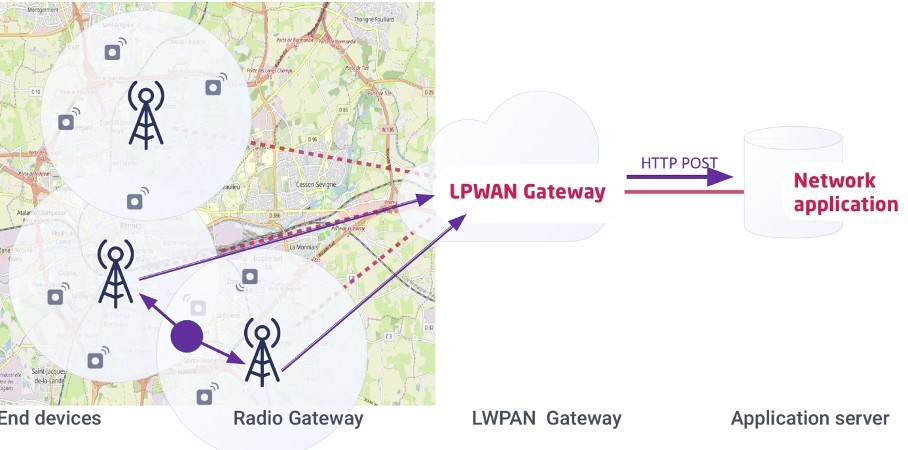
\includegraphics[width=1\columnwidth]{Pictures/TolologieStar.jpg}}
\caption{Architecture simplifiée des réseaux LPWAN}
\label{fig-topo-star}
\end{figure}


L’appareil envoie des données brutes sur le réseau radio. Le signal radio est capté par une ou plusieurs passerelles radio, et la trame est envoyée à une passerelle réseau (\ac{LNS}  pour les réseaux \Index{LoRaWAN}, et \ac{SCEF} pour les réseaux \ac{3GPP}).

Le propriétaire de l’appareil a associé l’appareil à un connecteur dans le LPWAN \ac{NGW} qui peut être un \ac{URI}, une adresse de broker \ac{MQTT} ou une Web socket. Lorsque l’appareil envoie des données, il est relié à l’application par ce tunnel.

    \vspace{1em}


Certaines technologies telles que LoRaWAN ou Sigfox utilisent des bandes sans licence, imposant un cycle d’utilisation (\Index{Duty Cycle}) de 0,1 à 10 \% selon les canaux pour assurer l’équité entre les nœuds, empêchant ainsi qu'un équipement ne monopolise le canal de transmission. Comme cette restriction s’applique également à l’antenne du fournisseur, la communication entre le réseau et l’appareil est considérablement limitée.

L’utilisation principale de ces réseaux \ac{LPWAN} est la télémétrie où un appareil envoie régulièrement des informations ou une alarme de temps en temps (par exemple des capteurs de température). Le débit et la taille des messages est beaucoup plus réduit que dans le cas de réseaux maillés.

    \vspace{1em}

\section{Niveaux 1 et 2}

 Concernant le niveau 2, le but est de gagner en énergie lors des transmissions. Déjà on peut dire adieu à Ethernet car cela imposerait d'utiliser l'infrastructure filaire et donc on ne pourrait pas placer les objets où on veut, surtout s'ils se déplacent. Les communications par ondes radio sont privilégiées. 
 
 Pour l'Internet des objets, le \Index{Wi-Fi} est également trop gourmand en énergie. On lui préfère donc une évolution appelée \Index{IEEE 802.15.4} qui reprend son principe de fonctionnement mais l'adapte à un faible débit et à des trames de petite taille. En particulier pour économiser l'énergie, la portée est réduite à une dizaine de mètres et il faut généralement utiliser des relais pour atteindre une destination. 
 
 \Index{Bluetooth} a été adapté pour des objets avec une basse consommation \ac{BLE}. 
     \vspace{1em}

 Côté téléphonie cellulaire, les protocoles évoluent pour prendre en compte les objets. La norme 4G a intégrée les communications à plus bas débit. La 5G inclura une classe permettant des communications avec les objets économes en énergie et réduisant les temps de latence. 
 
\section{IP et couches d'adaptation}

  Au niveau 3, on va vers l'utilisation plus massive d'\ac{IPv6} puisque la version 4 a son espace d'adressage saturé. la taille de l’adresse est étendue sur 128 bits offrant $2^{96}$ fois plus d’adresses.
  
  \begin{figure}[tbp]
\centerline{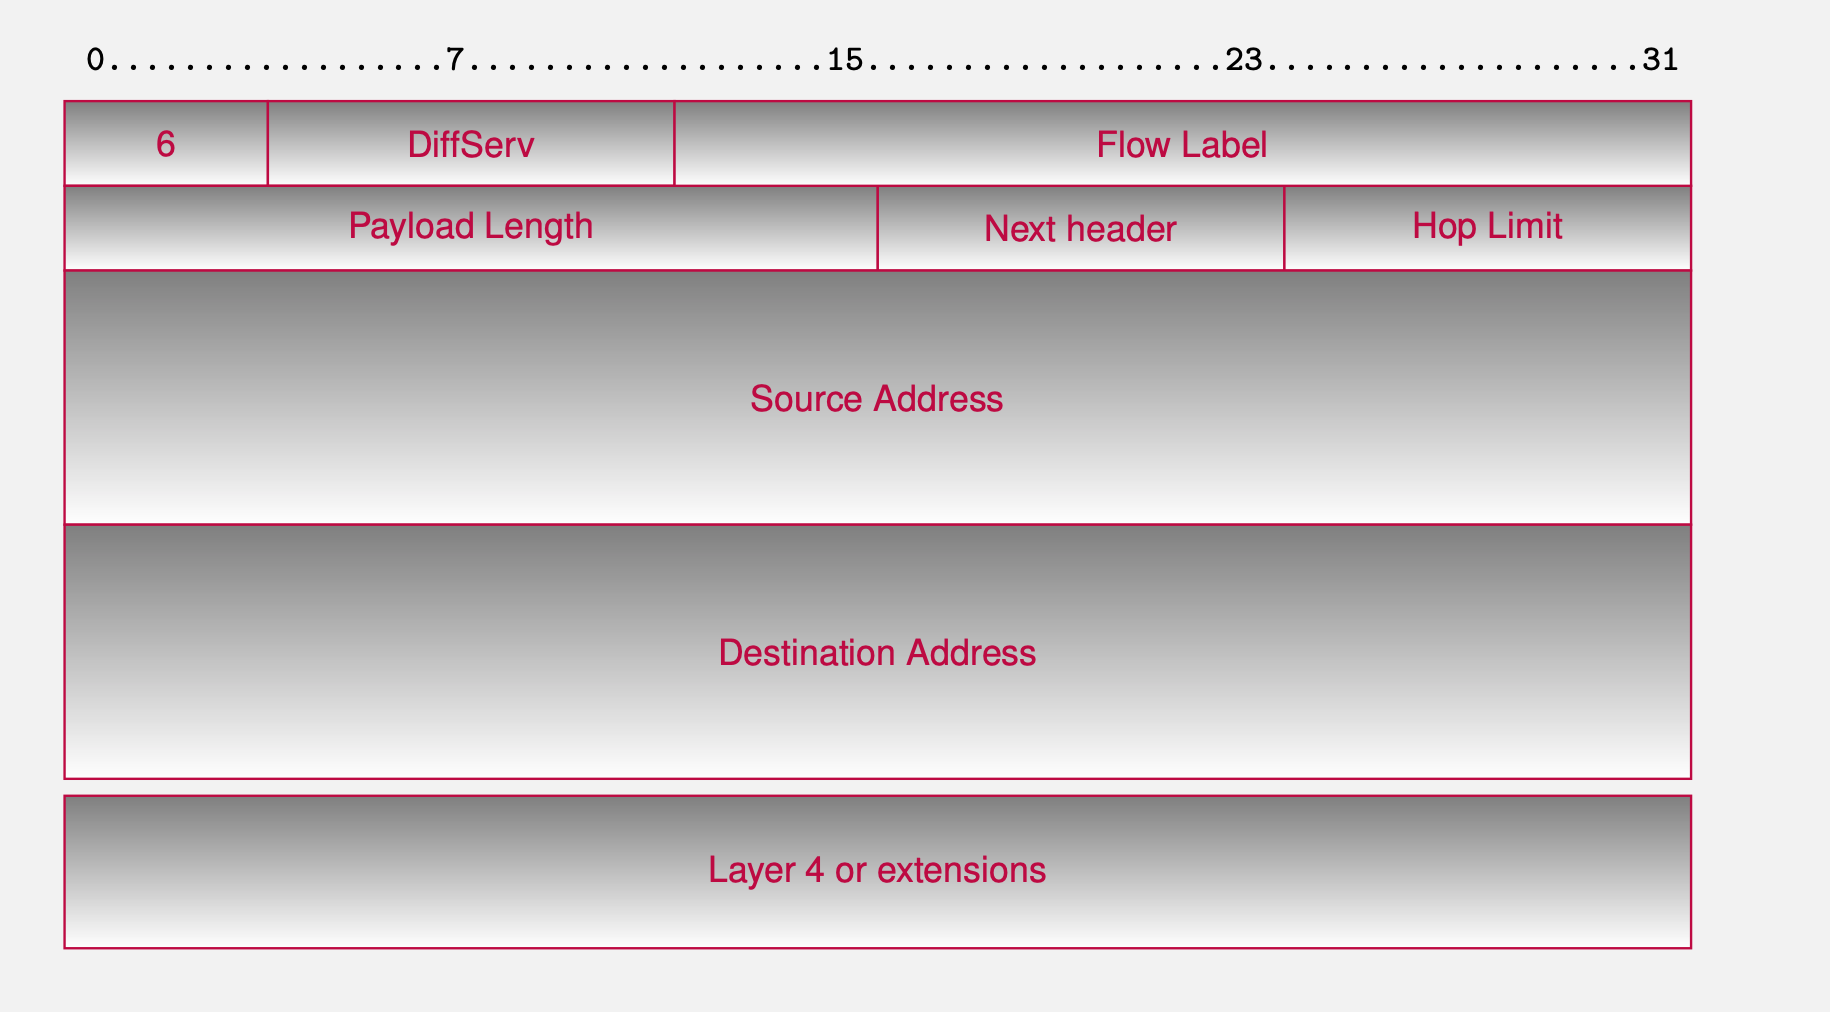
\includegraphics[width=1\columnwidth]{Pictures/Capture18.png}}
\caption{Format d'un en-tête IPv6}
\label{fig-IPv6-header}
\end{figure}

  
  
  
  
  
  Mais, comme on le voir sur la figure~\vref{fig-IPv6-header} \ac{IPv6} implique des en-têtes plus grandes, ce qui est gênant car les réseaux de niveau 2 transportent de plus petites trames.
  Une \Index{couche d'adaptation} entre la couche \ac{IP} et le niveau 2 est nécessaire puisque les niveaux 2 conçus pour l'internet des objets ne peuvent pas transporter naturellement de grands paquets. Deux actions sont mises en œuvre : \Index{compression} de la taille des en-têtes pour réduire leur impact, et \Index{fragmentation} pour découper le paquet en petites trames si la première mesure ne suffit pas. 


     \vspace{1em}

Il existe deux grandes familles de couche d'adaptation :

\begin{itemize}
 \item \Index{6LoWPAN} \rfc{4944}, \rfc{6282}, qui va intégrer un mécanisme de compression de l'en-tête \ac{IPv6} et de fragmentation pour envoyer un gros paquet divisé en petites trames. En effet, dans un réseau maillé, il n'est pas possible de se priver d'informations fournies par la couche \ac{IP} car les nœuds intermédiaires en ont besoin pour acheminer le message vers le destinataire. 
6LoWPAN est sans état et compresse toutes les en-têtes IPv6 sans configuration. 
\item \ac{SCHC} (prononcer chic) \rfc{8724} va imposer des règles décrivant l'en-tête du message et va envoyer le numéro de la règle en remplacement de l'en-tête. La compression est beaucoup plus importante et peut porter sur plusieurs couches protocolaires. Cependant, pour la mettre en œuvre, il faut avoir une idée des flux qui vont circuler sur le réseau. \ac{SCHC} est spécifié pour les réseaux en \Index{étoile} et plus particulièrement les \ac{LPWAN}.

\end{itemize}

\section{Mise en \oe{}uvre de \Index{REST}}
  
  Au-dessus on avait vu que comme \ac{HTTP} était le protocole dominant, \ac{TCP} l'était aussi. Mais pour l'IoT ce n'est pas optimal. En effet TCP/HTTP sont des protocoles complexes qui demandent beaucoup de mémoire. Pour réduire l'impact de la pile protocolaire, l'\ac{IETF} a défini un nouveau protocole appelé \ac{CoAP} qui demande que quelques Kilo Octets pour fonctionner. \ac{CoAP} repose sur \ac{UDP} ce qui simplifie encore la mise en oeuvre. 
  
  
       \vspace{1em}

  Pour poursuivre dans l’intégration des objets dans l’internet, le protocole \ac{CoAP} \rfc{7252} se substitue à \ac{HTTP}. Il en reprend le mécanisme de nommage, d’utilisation des ressources, et les primitives de manipulation entre un client et un serveur.

La capacité de traitement du capteur et son alimentation  en énergie sont souvent très limitées. 
La grande force de \ac{CoAP} est d’être :
\begin{itemize}
\item facile à mettre en œuvre. Les mises en œuvre de \ac{CoAP} nécessitent peu de mémoire ;
\item entièrement compatible avec 
\ac{HTTP} et il est possible d’aller d’un 
protocole à l’autre au travers de  passerelles génériques, c’est-à-dire non liées 
à un usage particulier (comme le montre la figure~\vref{fig-encap}).
\end{itemize}
De ce fait, \ac{CoAP} va manipuler des ressources, identifiées par des \ac{URI}. Il est donc possible d'ancrer les données fournies par les objets dans l'écosystème actuel des communications entre ordinateurs, fortement structuré autour des principes REST.

     \vspace{1em}

La sécurité, en particulier le chiffrement des données, suit aussi les mêmes chemins que l’internet traditionnel. 
Il existe un chiffrement au-dessus d’\ac{UDP} qui, à l’instar
de \ac{HTTPS}, 
chiffre les échanges.
  
\section{Representation des données}

Pour la structuration des données, \ac{XML} n'est pas utilisée car il est trop bavard. \ac{JSON} est beaucoup plus efficace pour transporter des informations structurées. Il existe un équivalent binaire que nous verrons par la suite \ac{CBOR} qui est beaucoup plus performant, et simple à mettre en oeuvre est compatible avec JSON.

\section {Alternatives à REST}


Il n'est pas obligé de tout mettre en oeuvre tous les protocoles définis par l'IETF. Il est possible également d'y intégrer des protocoles spécifiés pour un métier. 

   \begin{wrapfigure}{r}{7cm}
\centerline{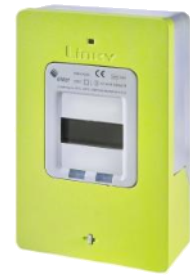
\includegraphics[width=.4\columnwidth]{Pictures/linky.png}}
\end{wrapfigure}

Par exemple, le compteur électrique \Index{Linky} que tous les Français connaissent en implémente qu'une partie. Au lieu d'utiliser \ac{CoAP}, les électriciens utilisent leurs propres applications suivant la norme \ac{DLMS}/\ac{Cosem}. Celle-ci repose sur \ac{UDP} puis \ac{IPv6} et \Index{6LoWPAN} et finalement sur une variante de \Index{IEEE 802.15.4} adaptée pour transporter l'information sur les câbles électriques.

\cleardoublepage

\lgf{\chapter{LA REPRESENTATION DE LA DONNEE}}
\lge{\chapter{THE REPRESENTATION OF DATA}}

\section{Introduction}
     \vspace{1em}

\lgf{Envoyer une donnée sur un réseau n’est pas aussi simple que l’on croit.}
\lge{Sending data over a network is not as simple as it seems.}
     \vspace{1em}

 \begin{wrapfigure}{r}{3cm}
\Youtube{https://youtu.be/k-RhgiwKx2M}
\end{wrapfigure}

\lgf{Il faut faire la différence entre le format utilisé pour stocker des données dans la mémoire de l'ordinateur et celui employé pour l'envoyer à une autre machine. En effet, chaque machine à sa propre représentation souvent liée aux capacités de leur processeur. Cela est surtout vrai pour les nombres. Ils peuvent être stockés sur un nombre de bits plus ou moins important ou peuvent être représentés en mémoire de manière optimisée pour accélérer leur traitement. }
\lge{There is a difference between the format used to store data in the computer's memory and the one used to send it to another machine. Indeed, each machine has its own representation often linked to the capacities of their processor. This is especially true for numbers. They can be stored on a more or less important number of bits or can be represented in memory in an optimized way to accelerate their treatment. }


\lgf{En revanche, la représentation des chaînes de caractères (non accentués) est relativement uniforme car elle se base sur le code ASCII qui est le même pour tous les ordinateurs. Un texte de base est facilement compréhensible par toutes les machines. Une solution serait donc de n'utiliser que des chaînes de caractères. }
\lge{On the other hand, the representation of (unaccented) character strings is relatively uniform because it is based on the ASCII code which is the same for all computers. A basic text is easily understandable by all machines. A solution would therefore be to use only strings of characters. }

     \vspace{1em}

\lgf{Par exemple, si l’on veut envoyer l'entier ayant pour valeur 123, il existe plusieurs représentations possibles :}
\lge{For example, if we want to send the integer with the value 123, there are several possible representations:}

\begin{itemize}
\item 
    \lgf{envoyer une chaîne de caractères ”123” contenant les chiffres du nombre ;}
    \lge{send a string "123" containing the digits of the number;}
\item 
    \lgf{envoyer la valeur binaire 1111011.}
    \lge{send the binary value 1111011.}
\end{itemize}

     \vspace{1em}

\lgf{On voit que juste pour transmettre une simple valeur stockée dans la mémoire d'un ordinateur, il existe plusieurs options et évidemment pour que cette valeur soit interprétée de la bonne façon, il faut que les deux extrémités se soient mises d'accord sur une représentation.}
\lge{We see that just to transmit a simple value stored in the memory of a computer, there are several options and obviously for this value to be interpreted in the right way, it is necessary that both ends have agreed on a representation.}

\lgf{Quand on veut transmettre plusieurs valeurs, c'est-à-dire quand on a des données structurées, d'autres problèmes surviennent.}
\lge{When you want to transmit several values, i.e. when you have structured data, other problems arise.}

\lgf{Par exemple : quelle est la taille des blocs que l’on va transmettre ? Comment indiquer la fin de la transmission ? Pour une chaîne de caractères, comment indiquer qu’elle se termine ? Autre exemple : si l'on veut transmettre "12" puis "3", comment faire pour que l'autre extrémité ne comprenne pas "123" ?}
\lge{For example: what is the size of the blocks we are going to transmit? How to indicate the end of the transmission? For a string, how to indicate that it ends ? Another example : if we want to transmit "12" and then "3", how do we make sure that the other end does not include "123"?}

     \vspace{1em}


\lgf{Pour que la transmission se fasse correctement, il faut que l’émetteur et le récepteur adoptent les mêmes conventions. Quand il s’agit d’un ensemble de données, il faut être capable de les séparer. Avec les tableurs, une première méthode est possible avec la notation \ac{CSV} Comme son nom l’indique, les valeurs sont séparées par des virgules. Les valeurs sont représentées par des chaînes de caractères. Les textes sont différenciés des valeurs numériques, par l’utilisation de guillemets. Ainsi, 123 sera interprété comme un nombre et ”123” comme un texte.}
\lge{In order for the transmission to take place correctly, the sender and receiver must adopt the same conventions. When it is a question of a set of data, it is necessary to be able to separate them. With spreadsheets, a first method is possible with the notation \ac{CSV} As its name indicates, the values are separated by commas. The values are represented by strings. The texts are differentiated from the numerical values by the use of quotation marks. Thus, 123 will be interpreted as a number and "123" as a text.}

\lgf{Si cette représentation est adaptée aux tableurs, elle est relativement pauvre car elle ne permet de représenter que des valeurs sur des lignes et des colonnes. Pour les usages du Web, il a fallu trouver un format plus souple permettant de représenter des structures de données complexes. Évidemment, comme rien n'est simple, il en existe plusieurs et les applications échangeant des données devront utiliser le même.}
\lge{If this representation is adapted to spreadsheets, it is relatively poor because it only allows to represent values on rows and columns. For Web uses, it was necessary to find a more flexible format allowing to represent complex data structures. Obviously, as nothing is simple, there are several of them and applications exchanging data will have to use the same one.}


     \vspace{1em}


\lgf{On voit que l'envoi de la chaîne de caractères ne suffit pas, il faut la formater pour que le récepteur puisse trouver le type de la donnée transmise, qu'un nombre ne soit pas interprété comme une chaîne de caractères, qu'une chaîne de caractères reste une chaîne de caractères même si elle ne contient que des chiffres.  }
\lge{We can see that sending the string is not enough, it must be formatted so that the receiver can find the type of the transmitted data, so that a number is not interpreted as a string, so that a string remains a string even if it contains only numbers.  }

    \vspace{1em}
   
\lgf{\section{La \Index{sérialisation}}}
\lge{\section{The \Index{serialization}}}

\lgf{Sous ce nom barbare se cache la méthode utilisée pour transmettre 
des données d’un ordinateur à un autre. Une donnée peut être simple (un nombre, un texte) ou plus complexe (un tableau, une structure...).  Elle est stockée dans la mémoire de l'ordinateur suivant une représentation qui lui est propre. Par exemple, la taille des entiers peut varier d'une technologie de processeur à une autre, l'ordre des octets dans un nombre peut aussi être différente (little et big endian).  Pour des structures complexes comme les tableaux, les éléments peuvent être rangés à différents emplacements de la mémoire. }
\lge{Under this barbaric name hides the method used to transmit 
data from one computer to another. A data can be simple (a number, a text) or more complex (an array, a structure...). It is stored in the computer's memory according to a representation that is specific to it. For example, the size of integers can vary from one processor technology to another, the order of bytes in a number can also be different (little and big endian).  For complex structures such as arrays, the elements can be stored in different locations in the memory. }


\lgf{La sérialisation consiste à transformer une structure de données en une séquence qui pourra être transmise sur le réseau, stockée dans un fichier ou une base de données. L'opération inverse, consistant à reconstruire localement une structure de données, s'appelle désérialisation.}
\lge{Serialization consists of transforming a data structure into a sequence that can be transmitted over the network, stored in a file or a database. The opposite operation, consisting in locally reconstructing a data structure, is called deserialization.}

\lgf{Il existe plusieurs formats pour sérialiser les données. Ils peuvent être binaires mais ceux généralement utilisés sont basés sur des chaînes de caractères. En effet, la représentation \ac{ASCII} définissant les caractères de base et codée sur 7 bits est commune à l'ensemble des ordinateurs. L'autre avantage du code ASCII est qu'il est facilement lisible et simplifie la mise au point des programmes.  }
\lge{There are several formats for serializing data. They can be binary but those generally used are based on character strings. Indeed, the representation \ac{ASCII} defining the basic characters and coded on 7 bits is common to all the computers. The other advantage of the ASCII code is that it is easily readable and simplifies the development of programs.  }

\lgf{Wikipédia donne ce tableau (cf. figure~\vref{fig-ASCII}) des codes \ac{ASCII} datant de 1972 (une éternité en informatique) et recolorisé par nos soins.}
\lge{Wikipedia gives this table (cf. figure~ref{fig-ASCII}) of the codes dating from 1972 (an eternity in computing) and recolored by us.}


\begin{figure}[tbp]
\centerline{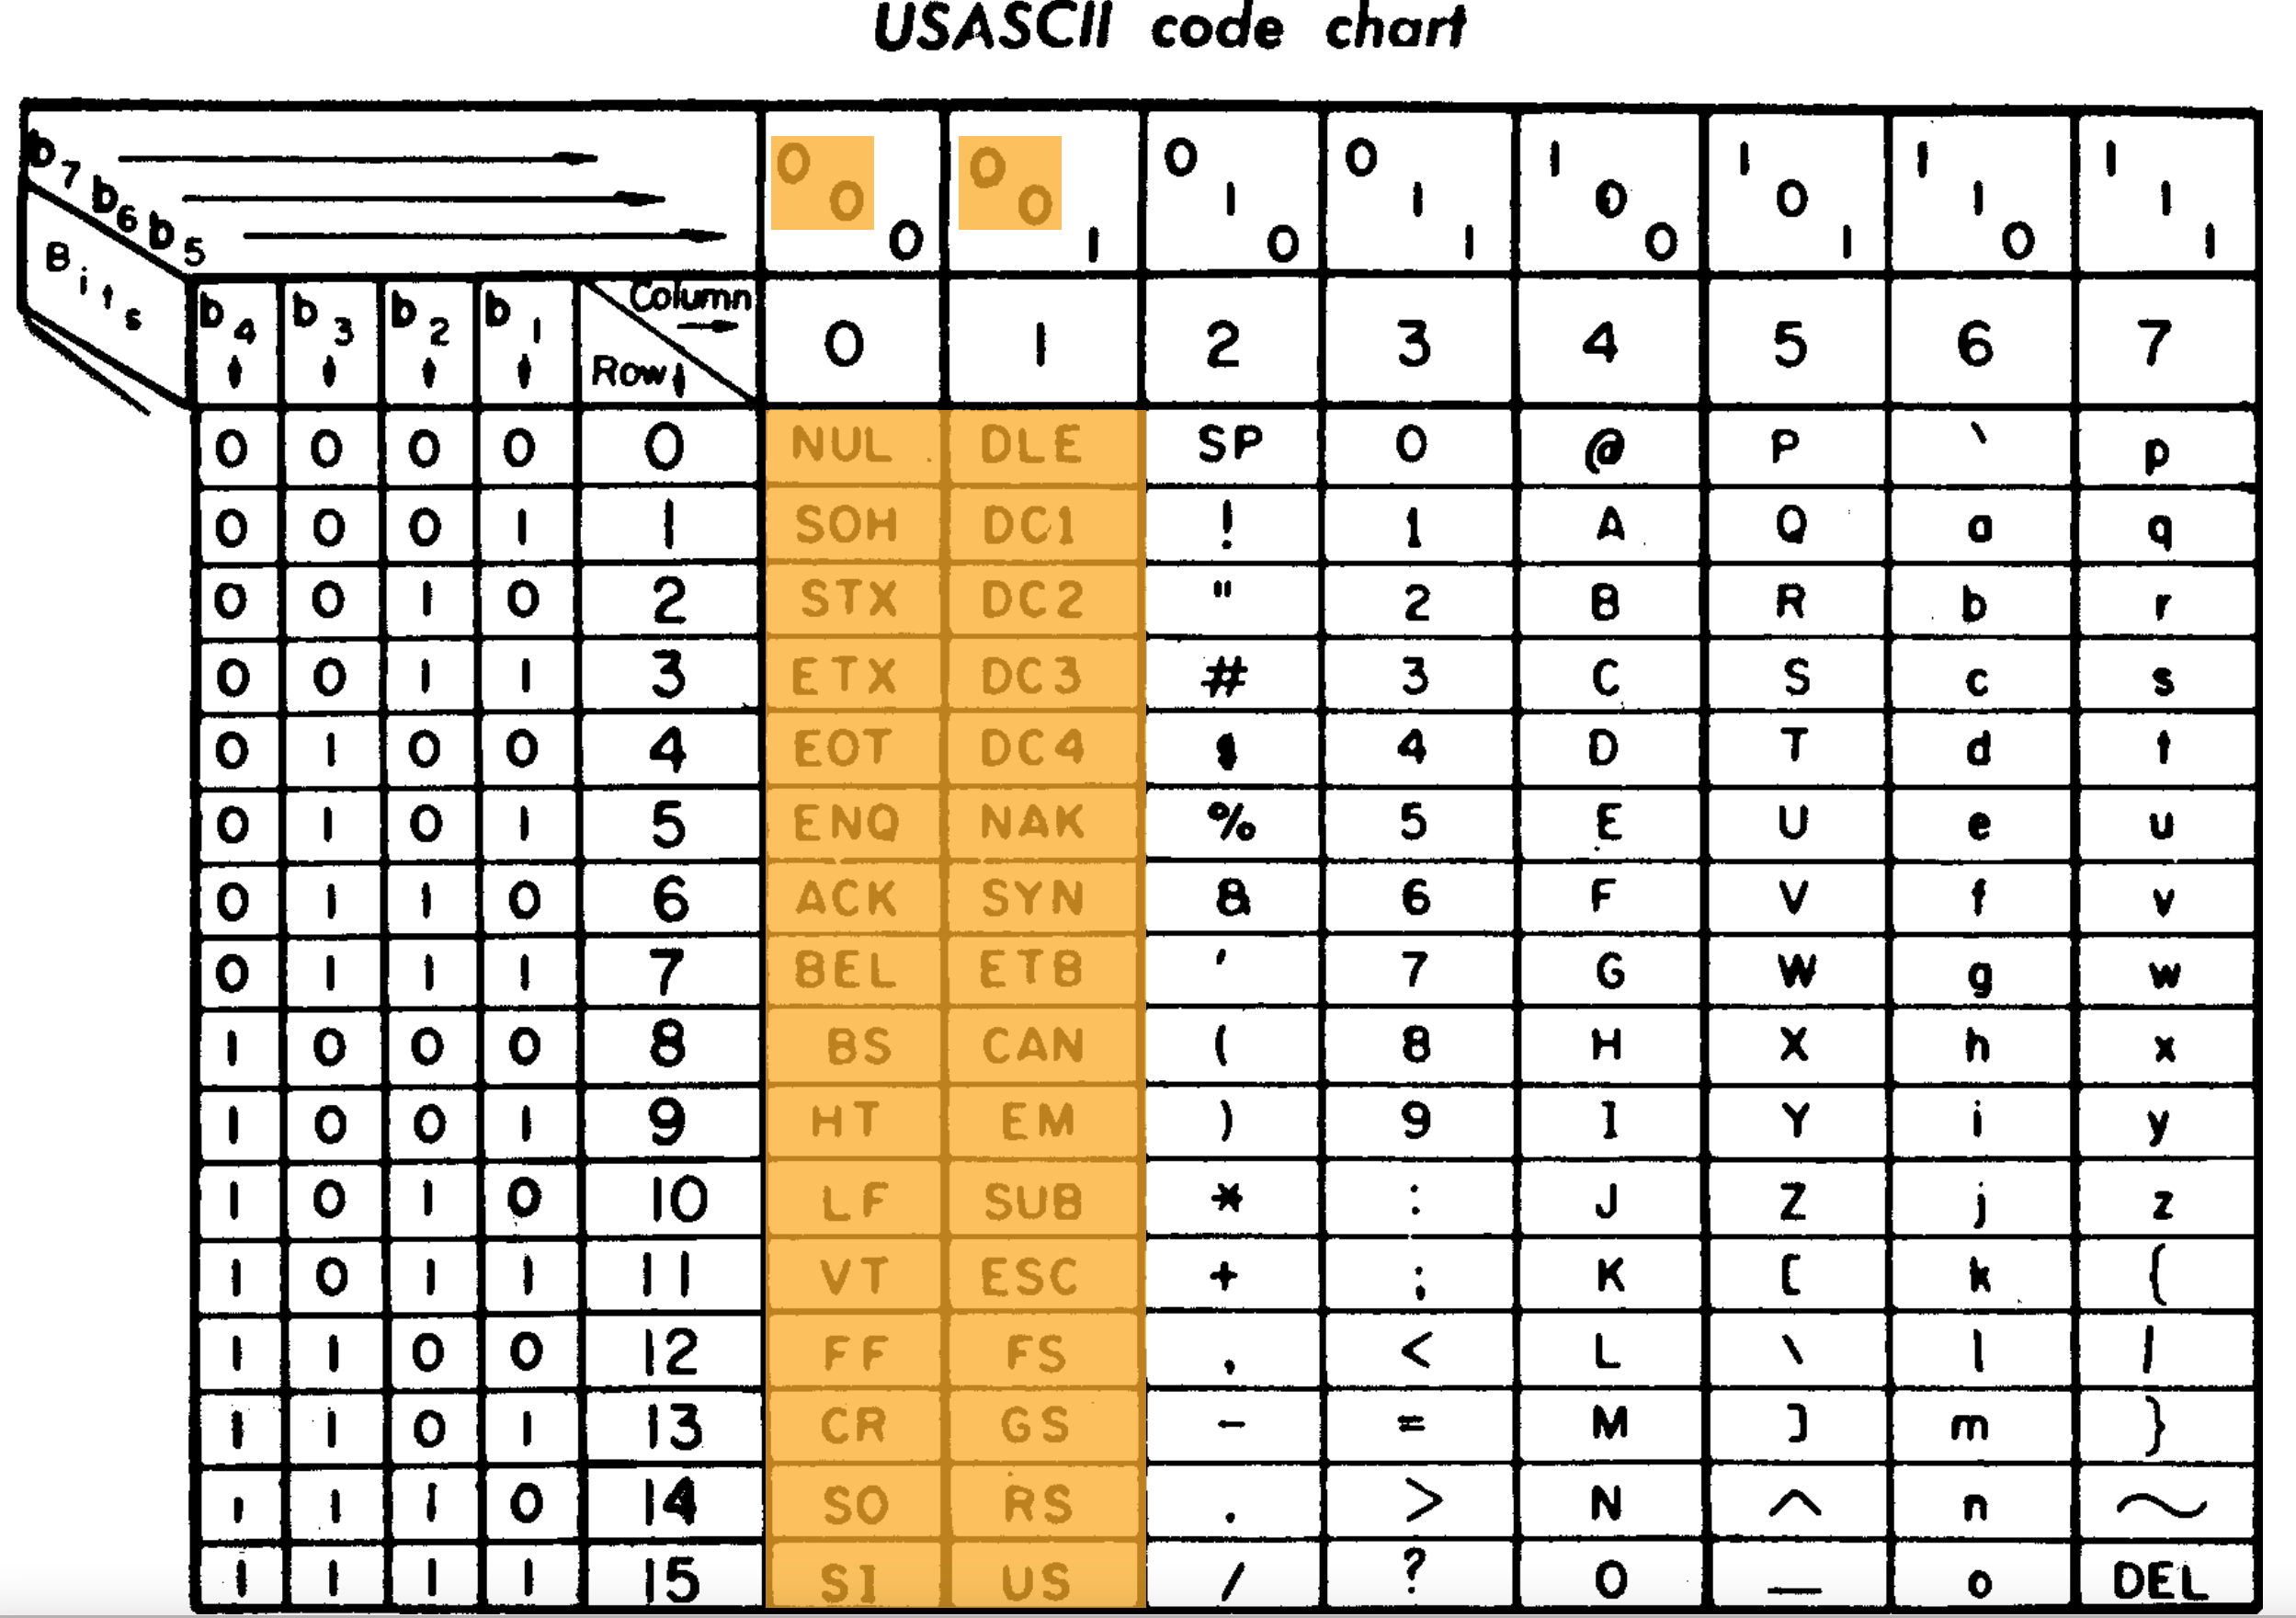
\includegraphics[width=1\columnwidth]{Pictures/Capture20.png}}
\lgf{\caption{Codage ASCII des caractères}}
\lge{\caption{ASCII character encoding}}
\label{fig-ASCII}
\end{figure}

\lgf{Les caractères en orange ne sont pas imprimables. Ils permettent de contrôler la communication des données ou de gérer l'affichage en revenant à la ligne. On les reconnait car la séquence binaire commence par 00X XXXX. On rappelle que le code ASCII est sur 7 bits ; le bit supplémentaire (bit de parité) conduisant à 1 octet était utilisé pour détecter des erreurs de transmission. Les valeurs de 0x30 à 0x39 codent les chiffres de 0 à 9. }
\lge{The characters in orange are not printable. They are used to control data communication or to manage the display by returning to the line. They can be recognized because the binary sequence starts with 00X XXXX. One recalls that the ASCII code is on 7 bits; the additional bit (parity bit) leading to 1 byte was used to detect transmission errors. The values from 0x30 to 0x39 code the digits from 0 to 9. }

\subsection*{Hexlify}

\lgf{En Python, il existe le module \Index{binascii} très pratique qui permet de convertir une séquence binaire en une chaîne de caractères ou inversement :}
\lge{In Python, there is the module \Index{binascii} very practical which makes it possible to convert a binary sequence into a character string or conversely:}
\begin{itemize}
\item 
    \lgf{\pfunction{binascii}{hexlify} prend un tableau d'octets et le convertit en une chaîne de caractères hexadécimaux plus lisible pour les spécialistes. Cela permet de visualiser n'importe quelle séquence de données. }
    \lge{\pfunction{binascii}{hexlify} takes an array of bytes and converts it to a more specialist-readable hexadecimal string. This allows you to view any sequence of data. }
\item 
    \lgf{\pfunction{binascii}{unhexify} fait l'inverse. Il prend une chaîne de caractères et la convertit en un tableau d'octets. Cela peut vous faciliter la programmation car, dans votre code, il est plus facile de manipuler des chaînes de caractères.}
    \lge{\pfunction{binascii}{unhexify} does the opposite. It takes a string and converts it to an array of bytes. This can make programming easier for you because in your code it is easier to manipulate strings.}

\end{itemize}
\lgf{Dans la suite, nous l'utiliserons pour manipuler des identifiants. Par exemple, ce bout de code illustre l'utilisation de ces fonctions :}
\lge{In the following, we will use these functions to manipulate identifiers. For example, this piece of code illustrates the use of these functions:}

\begin{python}
mac = lora.mac()
print ('devEUI: ',  binascii.hexlify(mac))

# create an OTAA authentication parameters
app_eui = binascii.unhexlify('70 B3 D5 7E D0 03 3A E3'.replace(' ',''))

\end{python}

\lgf{Comme nous le verrons par la suite, a fonction \pfunction{network}{lora.mac()} retourne un tableau d'octets. La fonction \pfunction{binascii}{hexlify} ligne suivante le convertit en chaîne de caractères pour un affichage plus propre. }
\lge{As we will see later, the function \pfunction{network}{lora.mac()} returns an array of bytes. The function \pfunction{binascii}{hexlify} in the follwoing line converts it to a string for a cleaner display. }

\lgf{Inversement, nous devons affecter une séquence binaire à la variable \texttt{app\_eui}. Nous mettons cette séquence hexadécimale en chaîne de caractères. Les espaces offrent plus de lisibilité. Ils sont retirés par la méthode replace et le résultat est converti en binaire grâce à \pfunction{binascii}{unhexify}}
\lge{Conversely, we must assign a binary sequence to the variable \texttt{app\_eui}. We put this hexadecimal sequence into a string. Spaces offer more readability. They are removed by the replace method and the result is converted into binary thanks to \pfunction{binascii}{unhexify}}

\section{Base64}

\lgf{Le passage d'une séquence binaire à une chaîne de caractères ASCII en représentant les valeurs conduit à un doublement du volume. Chaque bloc de 4 bits va conduire à produire un octet correspondant au caractère d'un chiffre ou d'une lettre de A à F. Le reste des codes n'est pas utilisé.}
\lge{The passage from a binary sequence to an ASCII character string representing the values leads to a doubling of the size. Each block of 4 bits will lead to produce a byte corresponding to the character of a digit or a letter from A to F. The rest of the codes are not used.}

\lgf{Le codage \Index{base64} offre un meilleur rendement en utilisant 64 bits pour coder les valeurs. Un dictionnaire fait la correspondance entre 64 valeurs et un caractère ASCII. Cependant, si l'on veut coder 4 octets, soit 32 bits, il faudra 5 blocs de 6 bits, et il y aura deux bits restants. Le symbole = indique que 2 bits sont ajoutés à la fin du codage. Donc, dans notre cas, il faudra ajouter deux symboles = comme le montre la figure ci-dessous :}
\lge{The encoding \Index{base64} offers a better performance by using 64 bits to encode the values. A dictionary maps 64 values to an ASCII character. However, if we want to encode 4 bytes, or 32 bits, we will need 5 blocks of 6 bits, and there will be 2 bits left. The symbol = indicates that 2 bits are added at the end of the coding. So, in our case, it will be necessary to add two symbols = as shown in the figure below:}

\begin{figure}[tbp]
\centerline{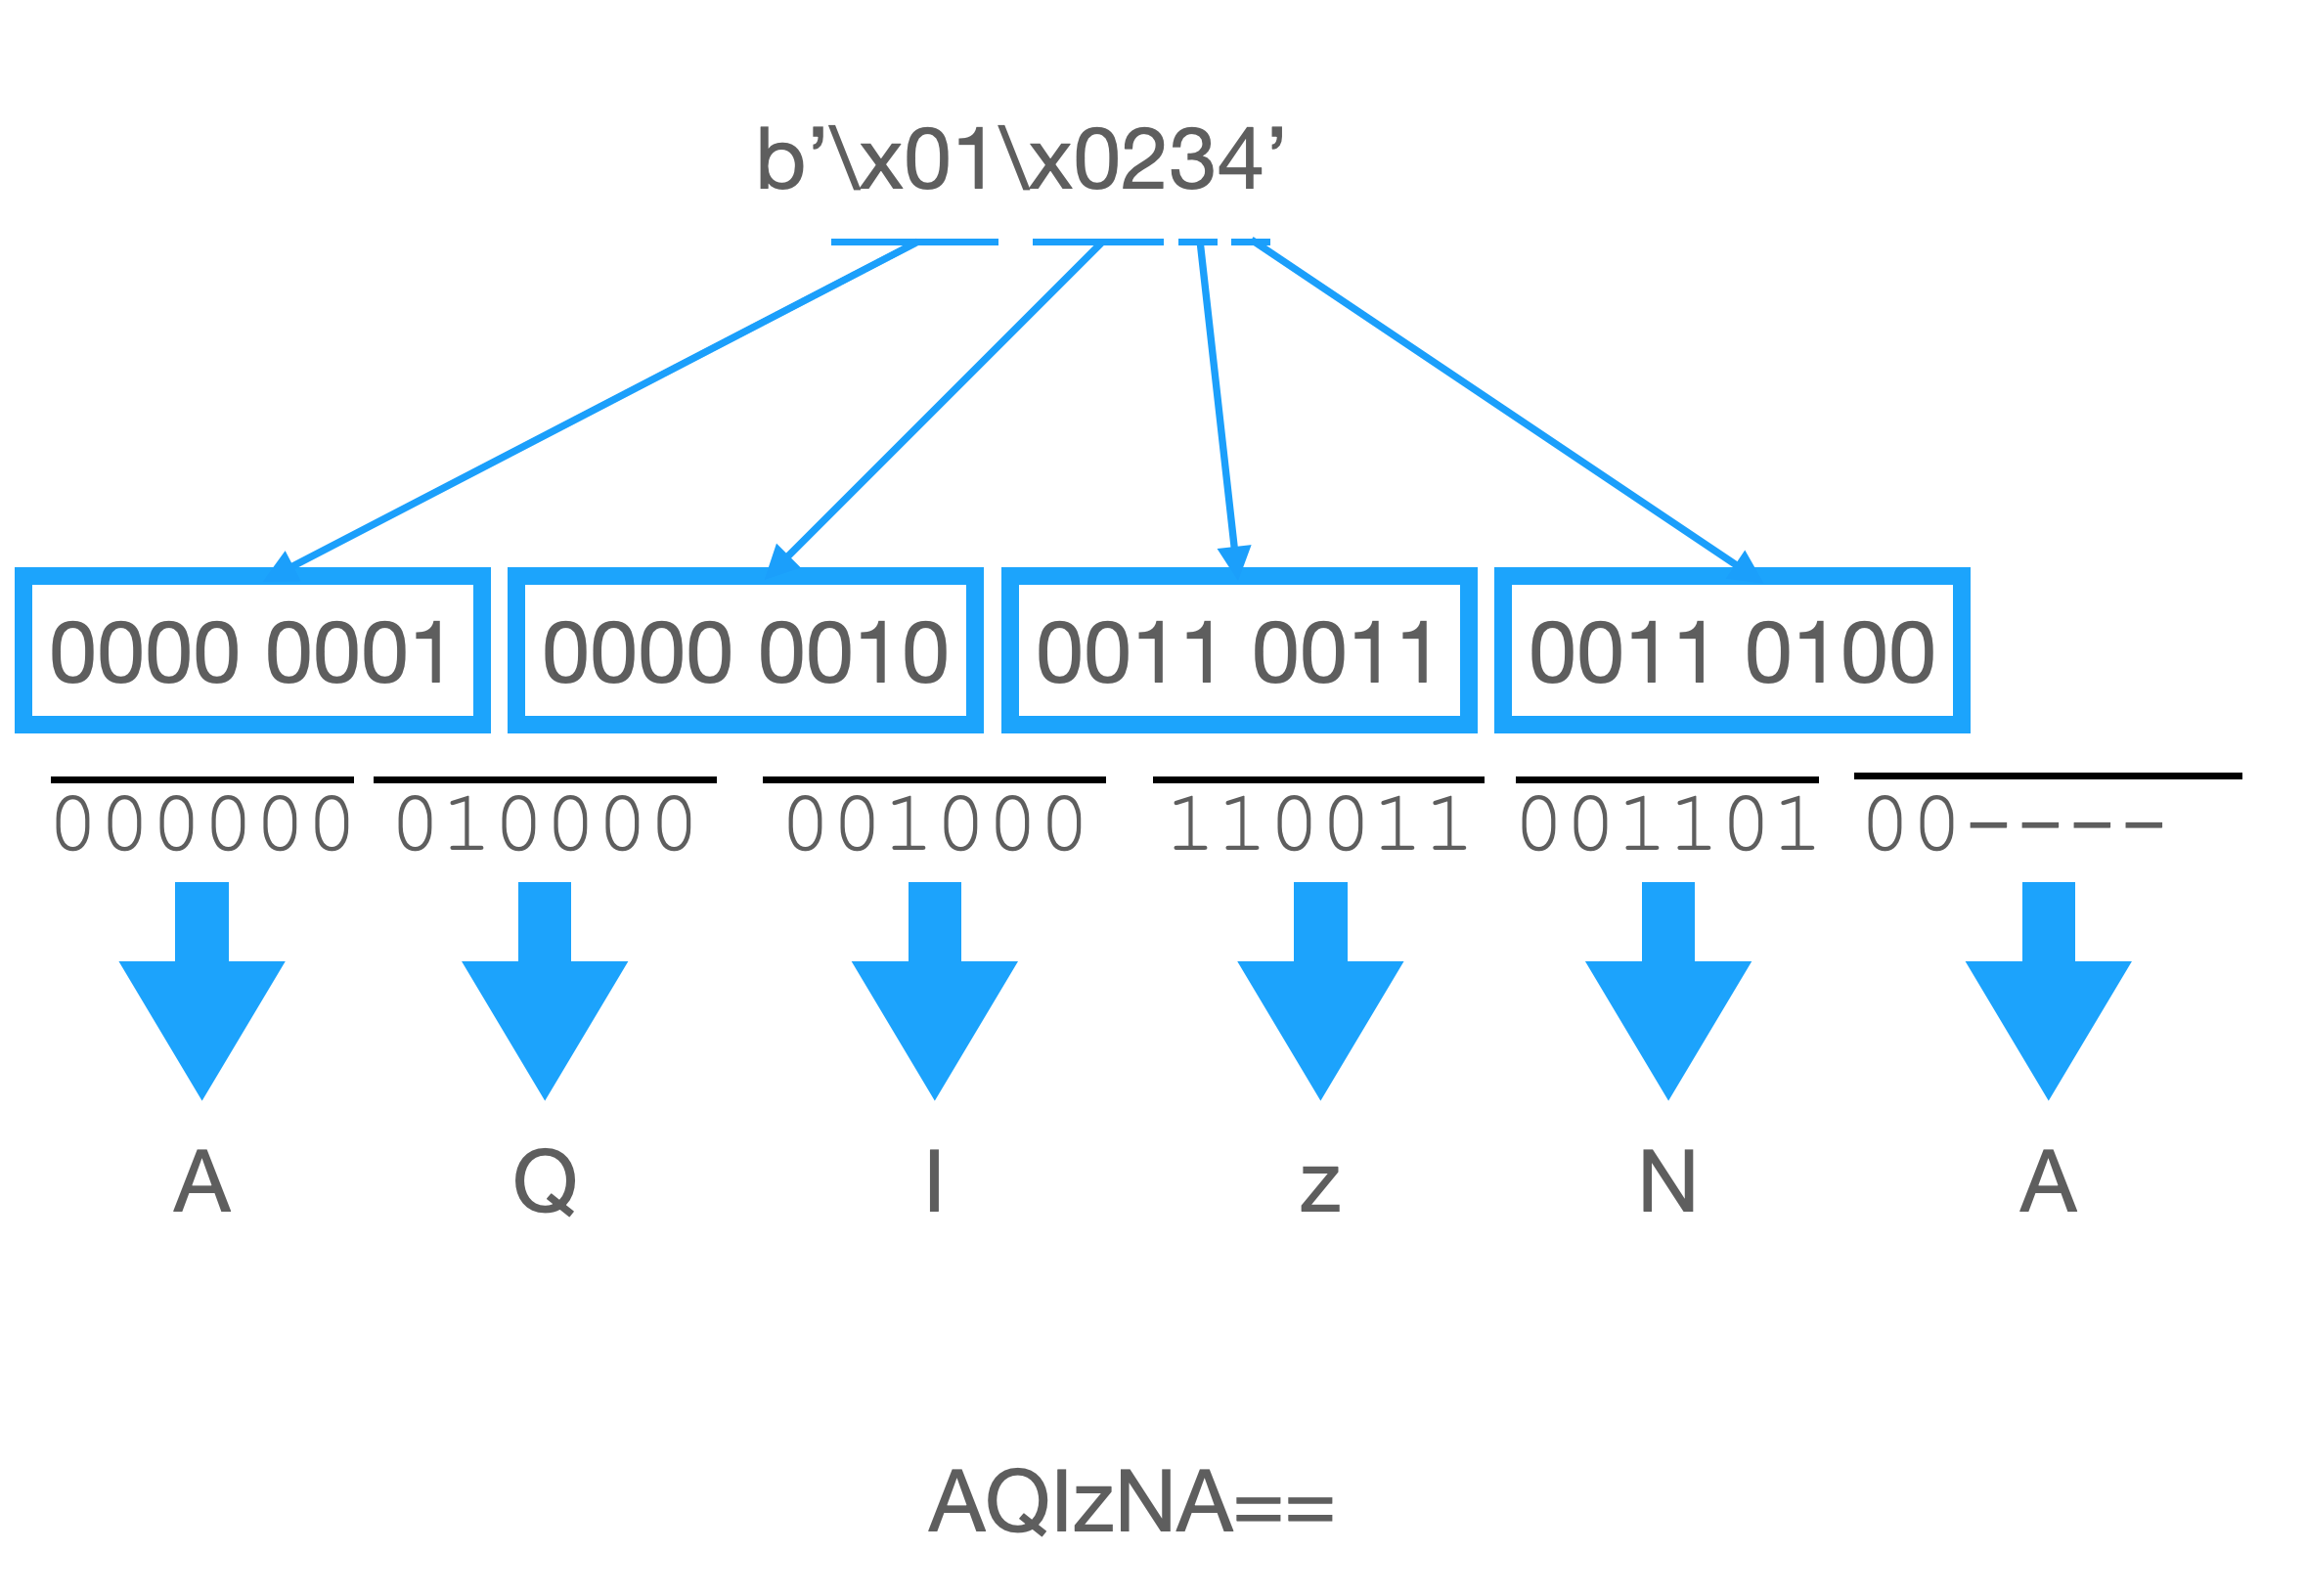
\includegraphics[width=1\columnwidth]{Pictures/Capture21.png}}
\lgf{\caption{Codage Base64 de données binaires}}
\lge{\caption{Base64 coding of binary data}}
\label{fig-base64}
\end{figure}

\lgf{On notera que pour les petites séquences, ce codage n'est pas meilleur que la transformation de la séquence hexadécimale en chaîne de caractères. Ici, il faut 8 caractères pour coder 4 octets. }
\lge{Note that for small sequences, this coding is not better than the transformation of the hexadecimal sequence into a string. Here, 8 characters are needed to encode 4 bytes. }

\lgf{Il existe beaucoup d'outils en ligne pour faire les conversions entre ces différentes représentations, comme le site \url{www.asciitohex.com}.}
\lge{There are many online tools to make conversions between these different representations, such as the site \url{www.asciitohex.com}.}

\lgf{\subsection*{Module Python : base64}}
\lge{\subsection*{Python module: base64}}

\lgf{En Python3, le module base64 permet de faire ces conversions.  Ce module est un peu susceptible sur les types de données à utiliser.}
\lge{In Python3, the base64 module allows to do these conversions.  This module is a bit touchy about the data types to use.}

\begin{python}[numbers=left,numbersep=5pt]
import base64

val = b"\x01\x0234"
ser = base64.b64encode(val)
print (ser)
print (ser.decode())
ori = base64.b64decode(ser)
print (ori)
\end{python}

\lgf{qui donne à l’exécution :}
\lge{which gives as a result of the execution :}

\begin{termc}[backgroundcolor=\color{backcolour}]
b'AQIzNA=='
AQIzNA==
b'\x01\x0234'
\end{termc}

\lgf{À noter que l'utilisation du \texttt{ser.\pfunction{str}{decode}()}, ligne 6, pour transformer une chaîne d'octets en chaîne de caractères, c'est-à-dire supprimer le \texttt{b} du début, peut être utilisé dans certains cas.}
\lge{Note that the use of \texttt{ser.\pfunction{str}{decode}()}, line 6, to transform a string of bytes into a string of characters, i.e. remove the \texttt{b} at the beginning, can be used in certain cases.}



\section{HTML}

\lgf{La sérialisation en chaînes de caractères (par exemple en Python via la commande \pfunction{binascii}{hexlify}) ou en Base64 concerne surtout des données binaires. Mais la donnée peut être aussi structurée, par exemple la page d'un tableur. Il faut donc formater le document pour éviter une fusion des différents champs.}
\lge{Serialization in strings (for example in Python via the command \pfunction{binascii}{hexlify}) or in Base64 concerns mainly binary data. But the data can also be structured, for example the page of a spreadsheet. The document must therefore be formatted to avoid merging the various fields.}


\lgf{\ac{HTML}, sans entrer dans les détails, définit un format où les champs sont repérés par un balisage.  Une balise de début est un mot clé entre \texttt{<>} et, pour une \Index{balise} de fin, le mot clé est précédé du caractère \texttt{/}. Par exemple, la figure~\vref{fig-HTML} avec le balisage, le premier paragraphe est formaté de cette manière dans le MOOC :}
\lge{\ac{HTML}, without going into detail,  defines a format where fields are marked up with markup.  A beginning tag is a keyword between \texttt{<>} and, for an ending \Index{tag}, the keyword is preceded by the character \texttt{/}. For example, the figure~\vref{fig-HTML} with the markup, the first paragraph is formatted this way in the MOOC:}


\begin{figure}[tbp]
\centerline{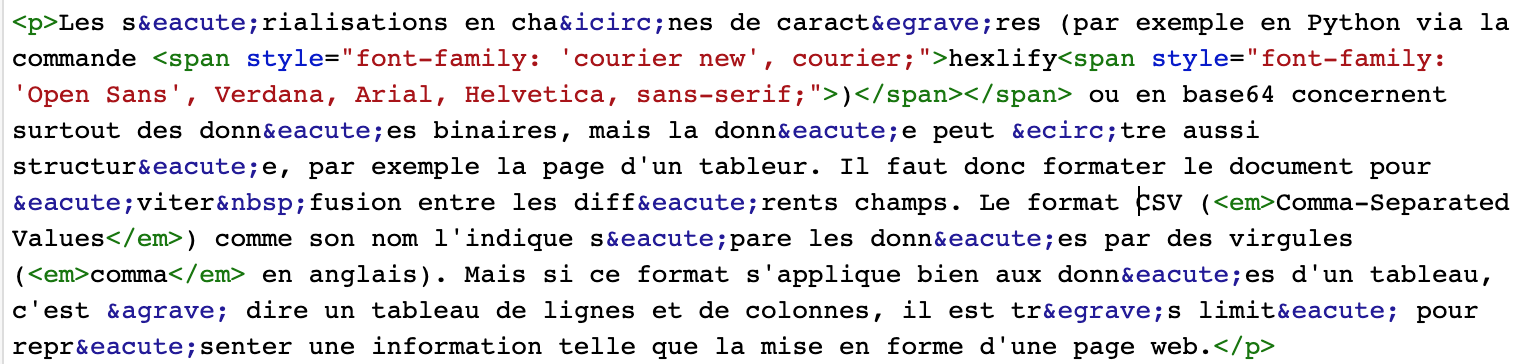
\includegraphics[width=1\columnwidth]{Pictures/Capture22.png}}
\lgf{\caption{Codage HTML d'une page Web}}
\lge{\caption{HTML coding of a Web page}}
\label{fig-HTML}
\end{figure}

\lgf{Les balises peuvent aussi prendre des arguments, comme la balise \Index{span} dans l'exemple précédent. Ainsi, si l'on regarde une page Web, comme indiqué figure~\vref{fig-Web-HTML}, le navigateur est capable de l'analyser pour trouver les \ac{URI} qu'elle contient. La balise \texttt{\Index{img}} indiquant qu'il s'agit d'une image, le client peut interroger le serveur pour l'afficher à l'écran. Ce format structuré de sérialisation nous permet de mettre en place une caractéristique de \ac{REST}, c'est-à-dire les liens entre ressources.}
\lge{Tags can also take arguments, like the \Index{span} tag in the previous example. Thus, if we look at a Web page, as shown in figure~\vref{fig-Web-HTML}, the browser is able to analyze it to find the \ac{URI} it contains. With the text tag indicating that it is an image, the client can query the server to display it on the screen. This structured serialization format allows us to implement a feature of \ac{REST}, i.e. the links between resources.}

\begin{figure}[tbp]
\centerline{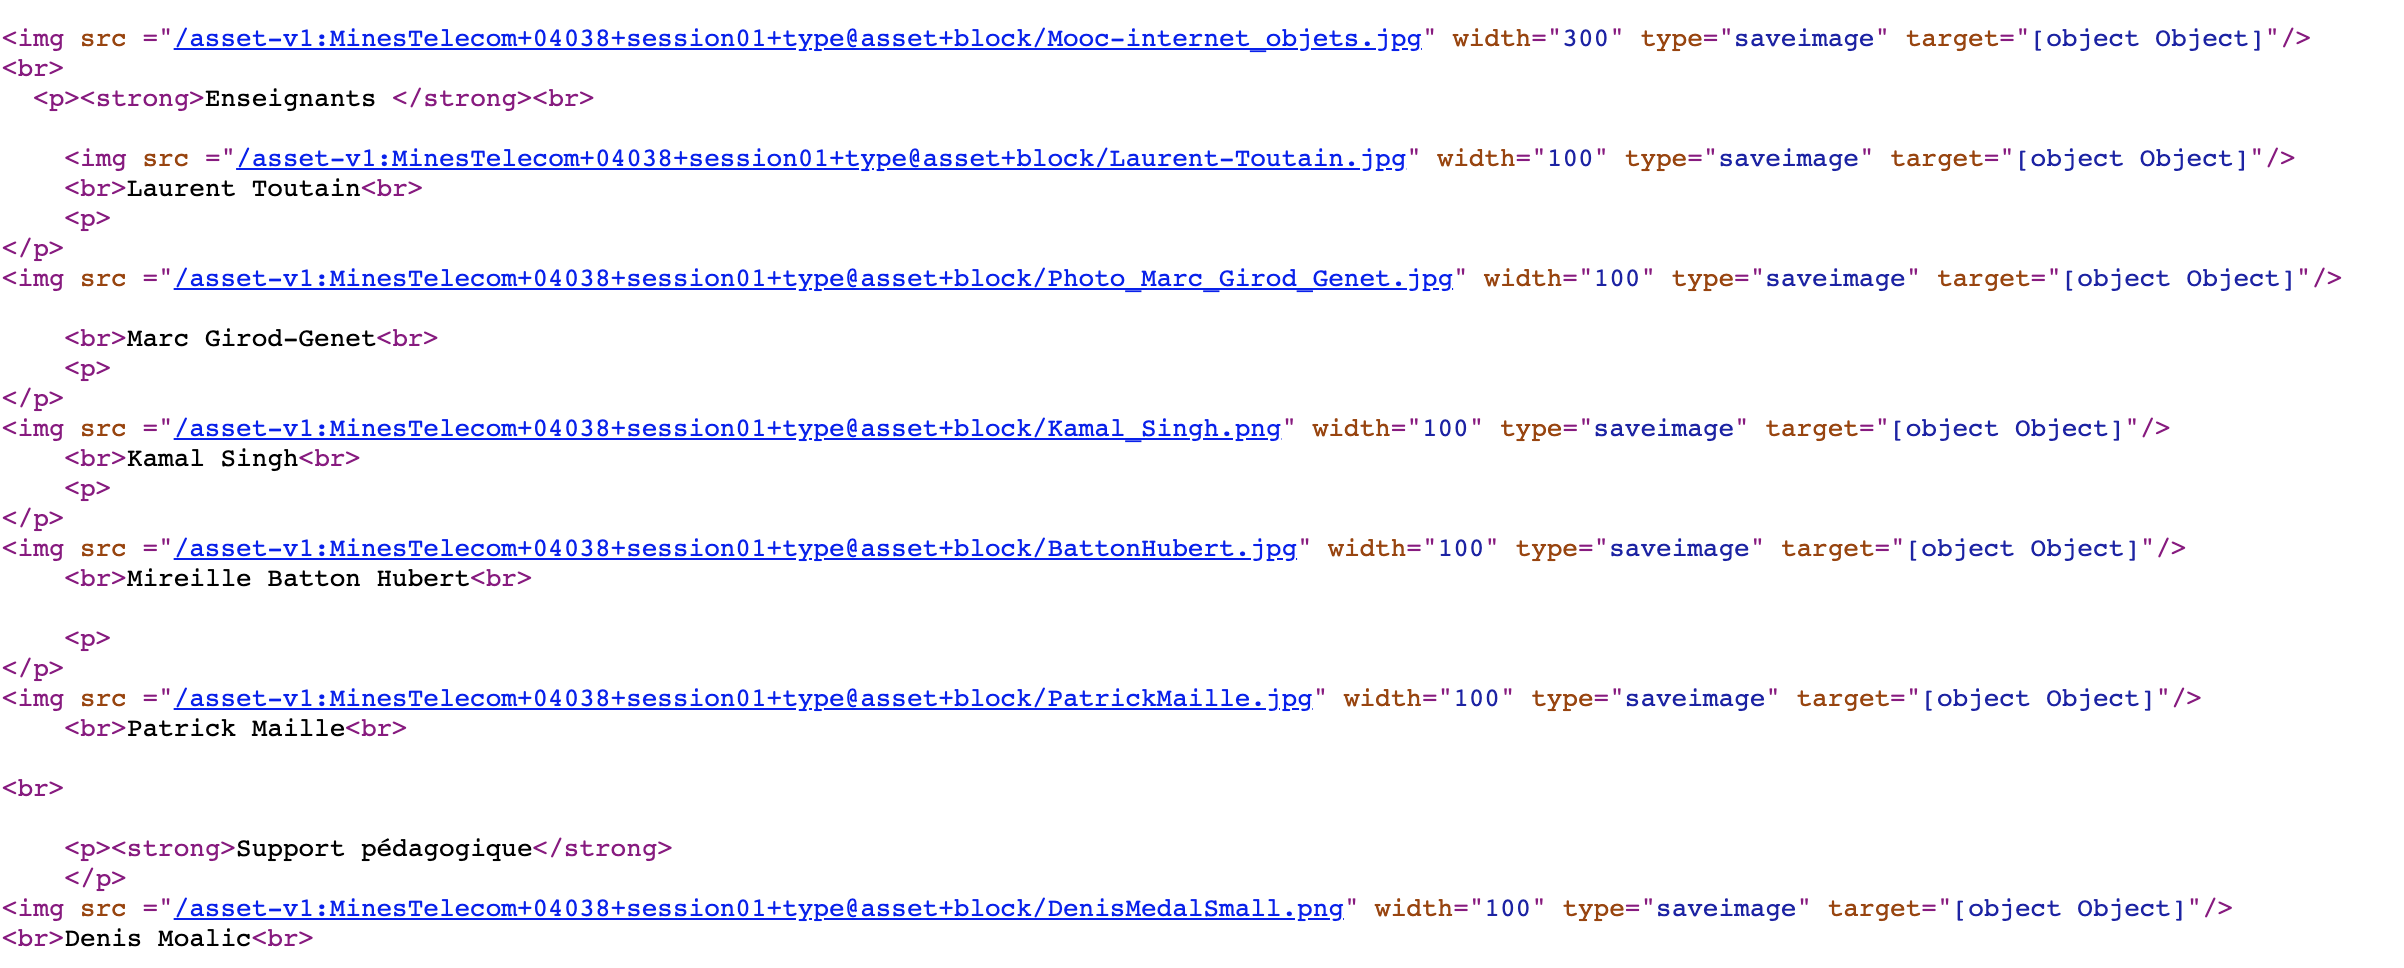
\includegraphics[width=1\columnwidth]{Pictures/Capture23.png}}
\lgf{\caption{Capture d'une page Web}}
\lge{\caption{Capture a web page}}
\label{fig-Web-HTML}
\end{figure}


\section{XML}

\lgf{Si \ac{HTML} est dédié au formatage à l'écran de données textuelles et à la navigation sur le Web. \ac{XML}\footnote{\url{https://www.w3.org/TR/xml/}} défini par le \ac{W3C}, est un format d’échange entre deux applications. Par exemple, pour échanger les notes des étudiants entre la plate-forme FUN et une autorité de certification des cours, on pourrait utiliser le format suivant~:}
\lge{If \ac{HTML} is dedicated to the formatting on screen of textual data and to the navigation on the Web. \ac{XML}\footnote{\url{https://www.w3.org/TR/xml/}} defined by the \ac{W3C}, is a format for exchange between two applications. For example, to exchange student grades between the FUN platform and a course certification authority, one could use the following format~:}

\begin{termc}[backgroundcolor=\color{palerod}]
<etudiant>
   <prenom>John</prenom>
   <nom>Deuf</nom>
   <note>18</note>
</etudiant>

\end{termc}

\lgf{Il est facile en lisant l'exemple de trouver le prénom, le nom et la note de l'étudiant. On peut noter qu'il n'y a pas de différence entre la note et le nom de l'élève. Il s'agit de caractères.}
\lge{It is easy by reading the example to find the student's first name, last name and grade. It can be noted that there is no difference between the grade and the student's name. They are characters.}

     \vspace{1em}

\lgf{S'il est syntaxiquement correct, rien ne dit que le créateur fournit quelque chose de correct qui pourra être interprété par une autre instance.  \ac{XML} peut inclure une grammaire ou un schéma qui est utilisé pour valider que les informations représentées dans le fichier sont non seulement syntaxiquement conformes au langage \ac{XML}, mais aussi conformes au schéma. Ce schéma va décrire les champs attendus et leur type (texte, nombre...). Vous pouvez accéder à ce cours si vous voulez en savoir plus sur les schémas \ac{XML}.}
\lge{If it is syntactically correct, there is no guarantee that the creator is providing something correct that can be interpreted by another instance.  \XML can include a grammar or schema that is used to validate that the information represented in the file is not only syntactically compliant with the language, but also complies with the schema. This schema will describe the expected fields and their type (text, number...). You can access this course if you want to know more about schemas.}

\lgf{Du point de vue de l’internet des objets, même si le XML pourrait être un bon candidat pour l’échange d’informations, il est un format trop lourd et donc énergivore. On peut noter que pour envoyer une note sur 20 qui, dans l'absolu, prendrait 6 bits, on transmet \texttt{<note>18</note>}, soit 15 caractères soit 120 bits! }
\lge{From the point of view of the Internet of Things, even if XML could be a good candidate for the exchange of information, it is too heavy a format and therefore energy consuming. We can note that to send a note out of 20 which, in the absolute, would take 6 bits, we transmit \texttt{<note>18</note>}, that is to say 15 characters or 120 bits! }

\section{JSON}

 \begin{wrapfigure}{r}{3cm}
\Youtube{https://youtu.be/IhZ9w6jWnq8}
\end{wrapfigure}

\lgf{\ac{JSON}  offre un moyen de structurer l’information de manière plus compacte que \ac{XML}. JSON s’impose comme le langage commun pour échanger les informations. A l’origine, JSON était utilisé par\Index{Javascriptt} pour échanger des informations ; par exemple, pour afficher en temps réel l’évolution des cours de la bourse ou pour afficher des graphiques dynamiques sur l’écran de l’utilisateur.}
\lge{\ac{JSON} offers a way to structure information in a more compact way than XML. JSON is emerging as the common language for exchanging information. Originally, JSON was used by \Index{Javascript} to exchange information; for example, to display in real time the evolution of stock exchange prices or to display dynamic graphs on the user's screen.}

\lgf{JSON \rfc{8259} est un format d’échange simple. Il définit 4 types de données :}
\lge{JSON \rfc{8259} is a simple exchange format. It defines 4 data types:}

\begin{itemize}
    \item 
        \lgf{nombre~: Les nombres sont composés de chiffres et peuvent être positifs, négatifs, entiers ou flottants.}
        \lge{Number: Numbers are composed of digits and can be positive, negative, integers or floats.}
    \item  
        \lgf{texte~: Le texte est délimité par des guillemets simples ou doubles.}
        \lge{Text: The text is delimited by single or double quotation marks.}
    \item  
        \lgf{\Index{tableau}~: Les tableaux sont des listes d’éléments séparés par des virgules et entourés de crochets.}
        \lge{\Index{Array}~: Arrays are lists of elements separated by commas and surrounded by square brackets.}
    \item  
        \lgf{\Index{objet}~: L’objet est une liste de paires composées d’une \Index{clé} et d’une valeur. La clé est une chaîne de caractères et la valeur peut être de n’importe quel type. La clé doit être unique à l’intérieur d’un objet, et référence entièrement la valeur qui la suit. Le couple clé - valeur est séparé par le caractère 2 points  \texttt{:}. Les éléments de l’objet sont séparés par des virgules. L'objet est délimité par des accolades.}
        \lge{\Index{Object}~: The object is a list of pairs composed of an \Index{key} and a value. The key is a string and the value can be of any type. The key must be unique within an object, and fully references the value that follows it. The couple key - value is separated by the colon character \texttt{:}. The elements of the object are separated by commas. The object is delimited by braces.}
\end{itemize}

\lgf{Par exemple, quelques structures \ac{JSON} :}
\lge{For example, some \ac{JSON} structures :}

\begin{itemize}
    \item 
        \lgf{\texttt{[1, -2, 0.3, 4e1]} est un tableau qui contient 4 nombres ;}
        \lge{\texttt{[1, -2, 0.3, 4e1]} is an array that contains 4 numbers;}
    \item  
        \lgf{\texttt{[1, ”2”, ”34”]} est un tableau contenant un nombre et deux chaines de caractères ;}
        \lge{\texttt{[1, "2", "34"]} is an array containing a number and two strings;}
    \item  
        \lgf{\texttt{[1, [2, 3 , ”4”]]} est un tableau de deux éléments dont le second est également un tableau de 3 éléments ;}
        \lge{\texttt{[1, [2, 3 , "4"]]} is an array of two elements whose second element is also an array of 3 elements;}
    \item  
        \lgf{\texttt{\{ ”couleur” : [34, 16, 3]\}} est un objet qui contient un élément et la valeur est un tableau ; }
        \lge{\texttt{\{ "color": [34, 16, 3]\}} is an object that contains an element and the value is an array; }
    \item  
        \lgf{\texttt{\{ ”name” : ”bob”, ”age” : 30\}} est un objet qui contient deux éléments référencés par les chaînes de caractères (ou index)  ”name” et ”age”.}
     
        \lgf{L’ordre dans lequel sont placés les éléments est indifférent. \texttt{\{”age” : 30, ”name” : ”bob”\}} est équivalent au dernier exemple. }
    
        \lgf{ Cela impose que l’index utilisé pour accéder à une valeur doit être unique dans la structure objet \texttt{\{”name” : ”bob”, ”name” : ”alice”}\} est interdit.}
        
        \lge{\texttt{ \{"name" : "bob", "age" : 30\}} is an object that contains two elements referenced by the strings (or index) "name" and "age".}
     
        \lge{The order in which the elements are placed is irrelevant. For example, \texttt{\{"age": 30, "name": "bob"\}} is equivalent to the last example. }
    
        \lge{This imposes that the index used to access a value must be unique in the object structure : \texttt{\{"name" : "bob", "name" : "alice"\}} is prohibited.}
\end{itemize}

     \vspace{1em}

\lgf{Le listing suivant donne un exemple de structure JSON tirée du \rfc{8259}. Il contient un objet JSON avec une seule clé \texttt{”Image”}. La valeur de cette clé est une autre structure qui contient six éléments. }
\lge{The following listing gives an example of a JSON structure from the \rfc{8259}. It contains a JSON object with a single key \texttt{"Image"}. The value of this key is another structure that contains six elements. }

\begin{termc}[backgroundcolor=\color{palerod}, language=json]
{
"Image": {
      "Width": 800,
      "Height": 600,
      "Title": "View from 15th Floor",
      "Thumbnail": {   
           "Url": "http://www.example.com/image/481989943",
           "Height": 125,
           "Width": 100
       },
       "Animated" : false,
       "IDs": [11, 943, 234, 38793]
    }
}
\end{termc}

\lgf{Le balisage par clé est un élément fondamental dans la structure des données. Il est primordial d'être cohérent et d'assurer une concordance entre émetteur et récepteur sur l'intitulé de la clé pour pouvoir récupérer l'information voulue. De la même façon, il faut s'accorder sur les unités de mesure : une interprétation d'une mesure en centimètre alors qu'elle est en pixel peut être désastreux ; c'est un problème d'interopérabilité.}
\lge{Key markup is a fundamental element in the structure of data. It is essential to be consistent and to ensure that the sender and receiver agree on the name of the key in order to be able to retrieve the desired information. In the same way, it is necessary to agree on the units of measurement: an interpretation of a measurement in centimeters when it is in pixels can be disastrous; it is an interoperability problem.}


     \vspace{1em}

\lgf{JSON est facilement exploitable dans d’autres langages. Par exemple en Python, le module JSON peut être utilisé pour convertir une structure JSON qui est une chaîne ASCII en une représentation interne Python. Les tableaux sont convertis en listes et les objets en dictionnaires.}
\lge{JSON is easily exploitable in other languages. For example in Python, the JSON module can be used to convert a JSON structure that is an ASCII string into a Python internal representation. Arrays are converted into lists and objects into dictionaries.}

     \vspace{1em}
     \pythonlst{example\_json.py}

\lgf{Le programme \pprog{example\_json.py}{cbor-example} reprend la structure précédente. La variable \texttt{struct\_python} est une structure Python. On peut voir que les valeurs pour \texttt{"Animated"} et \texttt{"Copyright"} sont les mots clé Python \texttt{False} (avec un F majuscule) et \texttt{None}. Le programme affiche deux fois cette valeur avec la commande standard \texttt{print} puis avec le module \pfunction{pprint}{pprint} pour avoir un affichage plus lisible. On peut remarquer que l'ordre d'affichage des clés est différent. Comme \texttt{"Title"} était défini deux fois, seul le dernier est conservé dans la structure Python.}
\lge{The program \pprog{example\_json.py}{cbor-example} uses the previous structure. The variable \texttt{struct\_python} is a Python structure. We can see that the values for \texttt{"Animated"} and \texttt{"Copyright"} are the Python keywords \texttt{False} (with a capital F) and \texttt{None}. The program displays this value twice with the standard command \texttt{print} then with the module \pfunction{pprint}{pprint} to have a more readable display. You can notice that the order of display of the keys is different. As \texttt{"Title"} was defined twice, only the last one is kept in the Python structure.}

\begin{termc}[backgroundcolor=\color{palerod}, language=json, basicstyle=\ttfamily\tiny]
{'Image': {'IDs': [17, 2371, 234, 38793], 'Height': 600, 'Animated': False, 'Title': 'Empty picture', 'Thumbnail': 
{'Url': 'http://www.example.com/image/481989943', 'Width': 100, 'Height': 125}, 'Width': 800, 'Copyright': None}}
{'Image': {'Animated': False,
           'Copyright': None,
           'Height': 600,
           'IDs': [17, 2371, 234, 38793],
           'Thumbnail': {'Height': 125,
                         'Url': 'http://www.example.com/image/481989943',
                         'Width': 100},
           'Title': 'Empty picture',
           'Width': 800}}
\end{termc}

\lgf{Grâce à la fonction \pfunction{json}{dumps} du module \texttt{json}, la variable \texttt{struct\_python} est transformée en JSON. Les mots clé  \texttt{False} et  \texttt{None} sont remplacés par  \texttt{false} et  \texttt{null}. Le programme affiche une chaîne de caractères.}
\lge{Thanks to the function \pfunction{json}{dumps} of the module \texttt{json}, the variable \texttt{struct\_python} is transformed into JSON. The keywords \texttt{False} and \texttt{None} are replaced by \texttt{false} and \texttt{null}. The program displays a string.}

\begin{termc}[backgroundcolor=\color{palerod}, language=json, basicstyle=\ttfamily\tiny]
{"Image": {"IDs": [17, 2371, 234, 38793], "Height": 600, "Animated": false, "Title": "Empty picture", "Thumbnail": 
{"Url": "http://www.example.com/image/481989943", "Width": 100, "Height": 125}, "Width": 800, "Copyright": null}}
\end{termc}

\lgf{Pour le retransformer, de JSON en variable Python, on utilise la fonction inverse \pfunction{json}{loads} qui traduit une chaîne de caractères en variable Python.}
\lge{To transform it back, from JSON to Python variable, we use the inverse function \pfunction{json}{loads} which translates a string into a Python variable.}

\begin{termc}[backgroundcolor=\color{palerod}, language=json, basicstyle=\ttfamily\tiny]
{'Image': {'Animated': False,
           'Copyright': None,
           'Height': 600,
           'IDs': [17, 2371, 234, 38793],
           'Thumbnail': {'Height': 125,
                         'Url': 'http://www.example.com/image/481989943',
                         'Width': 100},
           'Title': 'Empty picture',
           'Width': 800}}
\end{termc}


\lgf{Les autres langues de programmation possèdent également leur propre bibliothèque pour effectuer la traduction.}
\lge{Other programming languages also have their own libraries for translation.}

     \vspace{1em}

\lgf{Par rapport à \ac{XML}, \ac{JSON} est beaucoup plus permissif et manque de formalisme pour décrire la structure. \ac{JSON-LD} défini par le \ac{W3C} renforce l’interopérabilité de JSON en introduisant des clés spécifiques décrivant la structure des données, une référence aux unités, etc. Nous verrons ces concepts dans la suite du cours.}
\lge{Compared to \ac{XML}, \ac{JSON} is much more permissive and lacks a formalism to describe the structure. The \ac{JSON-LD} defined by the W3C reinforces the interoperability of JSON by introducing specific keys describing the data structure, a reference to units, etc. We will see these concepts in the rest of the course.}

\section{CBOR}

\begin{wrapfigure}{r}{3cm}
\Youtube{https://youtu.be/thSWuJ-1ld0}
\end{wrapfigure}

\lgf{\ac{JSON} et \ac{CBOR} sont tous les deux des modes de codage de la donnée.}
\lge{\ac{JSON} and \ac{CBOR} are both data encoding modes.}

\lgf{\ac{JSON} introduit une notation très flexible permettant de représenter toutes les structures de données. Le choix de l'\acs{ASCII} rend ce format universel et n'importe quel ordinateur pourra le comprendre. Mais l'utilisation de l'\acs{ASCII} ne permet pas de transmettre de manière optimale l'information sur un réseau. Quand les réseaux ont un débit raisonnable, cela ne pose pas de problème. Quand on en vient à l'internet des objets, il faut prendre en compte la capacité de traitement limité des équipements et la faible taille des messages échangés.}
\lge{\ac{JSON} introduces a very flexible notation allowing to represent all data structures. The choice of the \acs{ASCII} makes this format universal and any computer will be able to understand it. But the use of the \acs{ASCII} does not make it possible to transmit information in an optimal way on a network. When the networks have a reasonable flow, it does not pose a problem. When it comes to the Internet of Things, we must take into account the limited processing capacity of the equipment and the small size of the messages exchanged.}

     \vspace{1em}

\lgf{Ainsi, en ASCII, la valeur \texttt{123} est codée sur 3 octets (un octet par caractère) tandis qu'en binaire elle n'occuperait qu'un seul octet : \texttt{0111 1011}. }
\lge{Thus, in ASCII, the value \texttt{123} is coded on 3 bytes (one byte by character) while in binary it would occupy only one byte: \texttt{0111 1011}. }

      \vspace{1em}

\lgf{\ac{CBOR}, défini dans le \rfc{8949}, permet de représenter les structures de \ac{JSON} mais suivant une représentation binaire. Comme nous le verrons par la suite, si \ac{CBOR} est complètement compatible avec \ac{JSON}, il est possible de représenter d'autres types d'information très utiles dans l'Internet des Objets.}
\lge{\ac{CBOR}, defined in the \rfc{8949}, allows to represent the structures of \ac{JSON} but according to a binary representation. As we will see later, if \ac{CBOR} is completely compatible with \ac{JSON}, it is possible to represent other types of information very useful in the Internet of Things.}


\lgf{La taille de l'information est réduite et le traitement simplifié. Il faut savoir un peu jongler avec la représentation binaire mais cela reste basique.}
\lge{The size of the information is reduced and the processing simplified. You have to know how to juggle with the binary representation but it remains basic.}

      \vspace{1em}

\lgf{CBOR définit 8 types majeurs qui sont représentés par les 3 premiers bits d'une structure CBOR (cf. figure~\vref{fig-cbor-majeur}). Ces types majeurs ont donc des valeurs comprises entre 0 et 7 (\texttt{000} à \texttt{111} en binaire).}
\lge{CBOR defines 8 major types which are represented by the first 3 bits of a CBOR structure (cf. figure~\vref{fig-cbor-major}). These major types thus have values ranging from 0 to 7 (\texttt{000} to \texttt{111} in binary).}

\begin{figure}[tbp]
\centerline{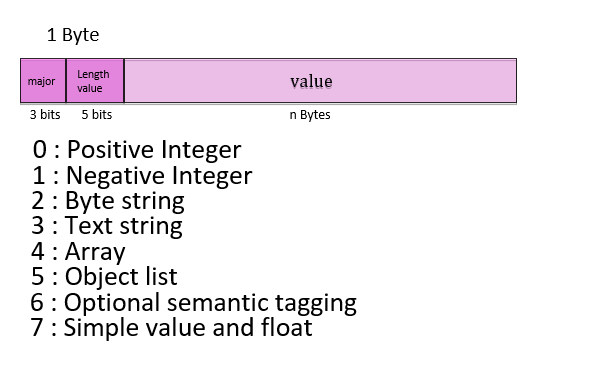
\includegraphics[width=1\columnwidth]{Pictures/cbor1.png}}
\lgf{\caption{Définition des majeurs en CBOR}}
\lge{\caption{Definition of major in CBOR}}
\label{fig-cbor-majeur}
\end{figure}


\lgf{Les cinq bits suivants contiennent soit une valeur soit une longueur indiquant combien d'octets sont nécessaires pour coder la valeur. \ac{CBOR} offre ainsi des optimisations qui permettent de réduire la longueur totale de la structure des données comme nous le verrons par la suite en étudiant les différents types majeurs.}
\lge{The next five bits contain either a value or a length indicating how many bytes are needed to encode the value. \Thus, this type offers optimizations that allow to reduce the total length of the data structure as we will see later when studying the different major types.}

\lgf{\subsection{CBOR en python}}
\lge{\subsection{CBOR in Python}}

\lgf{Les exemples qui vont suivre peuvent être testés sur votre ordinateur avec Python3. Si une erreur se produit au moment de la définition du module \texttt{\Index{cbor2}}, vous devez l'installer sur votre ordinateur en tapant la commande :}
\lge{The following examples can be tested on your computer with Python3. If an error occurs when defining the module \texttt{Index{cbor2}}, you must install it on your computer by typing the command :}

\begin{termc}[backgroundcolor=\color{gray!10}, language=json, basicstyle=\ttfamily\small, escapechar=@]
# @\texttt{pip3 install cbor2}@
\end{termc}


\lgf{\subsection{Type Entier Positif}}
\lgf{\subsection{Type Positive Integer}}


\lgf{\ac{JSON} ne fait pas de différence entre les nombres, entiers, décimaux, positifs ou négatifs. \ac{CBOR} réintroduit une distinction pour optimiser la représentation.}
\lge{\ac{JSON} does not make a difference between numbers, integers, decimals, positive or negative. \ac{CBOR} reintroduces a distinction to optimize the representation.}


      \vspace{1em}

\lgf{Le premier type majeur correspond aux entiers positifs. Il est codé par 3 bits à 0 ; les 5 bits suivants finissent l'octet et, suivant leur valeur, vont avoir une signification différente :}
\lge{The first major type corresponds to the positive integers. It is coded by 3 bits at 0; the 5 following bits end the byte and, according to their value, will have a different meaning:}

\begin{itemize}
    \item 
        \lgf{de 0 à 23, il s'agit de la valeur de l'entier à coder ;}
        \lge{from 0 to 23, it is the value of the integer to be coded;}
    \item 
        \lgf{24 indique que l'entier est codé sur 1 octet qui sera codé dans l'octet suivant ;}
        \lge{24 indicates that the integer is coded on 1 byte which will be coded in the following byte ;}
    \item 
        \lgf{25 indique que l'entier est codé sur 2 octets qui seront codés dans les deux octets suivants ;}
        \lge{25 indicates that the integer is coded on 2 bytes which will be coded in the two following bytes ;}
    \item 
        \lgf{26 indique que l'entier est codé sur 4 octets qui seront codés dans les quatre octets suivants ;}
        \lge{26 indicates that the integer is coded on 4 bytes which will be coded in the four following bytes ;}
    \item 
        \lgf{27 indique que l'entier est codé sur 8 octets qui seront codés dans les huit octets suivants.}
        \lge{27 indicates that the integer is coded on 8 bytes which will be coded in the eight following bytes.}
\end{itemize}

      \vspace{1em}

\lgf{On peut noter qu'il n'y a pas de surcoût pour coder un entier de 0 à 23. Ainsi, la valeur 15 sera codée 0x0F (\texttt{000-0 1111}) tandis que, pour toutes les autres valeurs supérieures, le surcoût ne sera que d'un octet. La valeur 100 sera codé \texttt{000-1 1000}\footnote{\texttt{11000} correspond à 24} suivi du codage sut 1 octet de la valeur 100 (\texttt{0110 0100}).}
\lge{One can note that there is no extra cost to code an integer from 0 to 23. Thus, the value 15 will be coded 0x0F (\texttt{000-0 1111}) while, for all the other higher values, the overcost will be only of one byte. The value 100 will be coded \texttt{000-1 1000}\footnote{\texttt{11000} corresponds to 24} followed by the coding on 1 byte of the value 100 (\texttt{0110 0100}).}



      \vspace{1em}

\pythonlst{cbor-integer-ex1.py}

\lgf{Le programme \pprog{cbor-integer-ex1.py}{cbor-example}  affiche les puissances de $10$ entre $10^0$ et $10^{18}$~:}
\lge{The program \pprog{cbor-integer-ex1.py}{cbor-example} displays the powers of $10$ between $10^0$ and $10^{18}$~:}

\begin{itemize}
    \item 
        \lgf{Ligne 1, le programme importe le module \texttt{\Index{cbor2}} et le renomme pour plus de simplicité \texttt{cbor}.}
        \lge{Line 1, the program imports the module \texttt{Index{cbor2}} and renames it for simplicity \texttt{cbor}.}
    \ligne  
        \lgf{Ligne 5, la boucle permet d'avoir les multiples de 10 (variable \texttt{v)}. }
        \lge{Line 5, the loop allows to have the multiples of 10 (variable \texttt{v)}. }
    \item  
        \lgf{Ligne 6, le module \texttt{cbor} utilise comme pour JSON la méthode \pfunction{cbor2}{dumps} pour sérialiser une structure interne de Python dans la représentation demandée. À l'inverse, la méthode \pfunction{cbor2}{loads} sera utilisée pour importer une structure CBOR dans une représentation interne.}
        \lge{Line 6, the module \texttt{cbor} uses as for JSON the method \pfunction{cbor2}{dumps} to serialize an internal Python structure into the requested representation. Conversely, the \pfunction{cbor2}{loads} method will be used to import a CBOR structure into an internal representation.}
    \item  
        \lgf{Ligne 7, le \texttt{print} permet d'aligner les données pour que l'affichage soit plus clair ; entre les accolades, le premier chiffre indique la position dans les arguments de format ; le second, après le \texttt{:}, le nombre de caractères. Par exemple, \texttt{\{1:30\}} indique l'argument \texttt{v} de format affiché sur 30 caractères.}
        \lge{On line 7, the \texttt{print} is used to align the data so that the display is clearer; between the braces, the first number indicates the position in the format arguments; the second, after the \texttt{:}, the number of characters. For example, \texttt{\{:1:30\}} indicates the format argument \texttt{v} displayed in 30 characters.}
\end{itemize}
 
       \vspace{1em}

\lgf{Le programme donne le résultat suivant~:}
\lge{The program gives the following result:}

\begin{termc}[backgroundcolor=\color{palerod}, language=json, basicstyle=\ttfamily\small, escapechar=@]
 # @\textbf{python3 cbor-integer-ex1.py}@
  0                              1 01
  1                             10 0a
  2                            100 1864
  3                           1000 1903e8
  4                          10000 192710
  5                         100000 1a000186a0
  6                        1000000 1a000f4240
  7                       10000000 1a00989680
  8                      100000000 1a05f5e100
  9                     1000000000 1a3b9aca00
 10                    10000000000 1b00000002540be400
 11                   100000000000 1b000000174876e800
 12                  1000000000000 1b000000e8d4a51000
 13                 10000000000000 1b000009184e72a000
 14                100000000000000 1b00005af3107a4000
 15               1000000000000000 1b00038d7ea4c68000
 16              10000000000000000 1b002386f26fc10000
 17             100000000000000000 1b016345785d8a0000
 18            1000000000000000000 1b0de0b6b3a7640000
\end{termc}

       \vspace{1em}


\lgf{On voit facilement que les valeurs 1 et 10 sont codées sur 1 octet ; que 100 est codé sur 2 octets tandis que les valeurs 1 000 et 10 000 sont codées sur 3 octets. Les valeurs entre 100 000 et 1 000 000 000 nécessitent 5 octets et les valeurs suivantes, 9 octets.}
\lge{It is easy to see that the values 1 and 10 are coded on 1 byte; that 100 is coded on 2 bytes while the values 1 000 and 10 000 are coded on 3 bytes. The values between 100 000 and 1 000 000 000 require 5 bytes and the following values, 9 bytes.}


       \vspace{1em}


\lgf{La taille de la représentation s'adapte à la valeur. Ainsi, il n'est pas nécessaire de définir une taille fixe pour coder une donnée.}
\lge{The size of the representation adapts to the value. Thus, it is not necessary to define a fixed size to encode a data.}

\lgf{On peut aussi noter que comme le type majeur est sur 3 bits, ce type peut être reconnu dans une lecture hexadécimale du résultat car la séquence commence toujours par le symbole \texttt{0} ou \textttt{1}.}
\lge{We can also note that as the major type is on 3 bits, this type can be recognized in a hexadecimal reading of the result because the sequence always starts with the symbol \texttt{0} or \textttt{1}.}

\lgf{\subsection{Type Entier Négatif}}
\lge{\subsection{Type Negative Integer}}


\lgf{Le type majeur entier négatif est à peu près similaire à l'entier positif. Le type majeur est \texttt{001} et le codage de la valeur se fait sur la valeur absolue du nombre à laquelle on retranche 1. Cela évite deux codes différents pour les valeurs 0 et -0.}
\lge{The major type negative integer is roughly similar to the positive integer. The major type is \texttt{001} and the encoding of the value is done on the absolute value of the number to which we subtract 1. This avoids two different codes for the values 0 and -0.}

       \vspace{1em}

\lgf{Ainsi, pour coder -15, on va coder la valeur 14, ce qui donne en binaire 001-1 1110. Ainsi, -24 peut également être codé sur 1 octet tandis que +24 sera codé sur 2 octets.}
\lge{Thus, to code -15, we will code the value 14, which gives in binary 001-1 1110. Thus, -24 can also be coded on 1 byte while +24 will be coded on 2 bytes.}

\pythonlst{cbor-integer-ex2.py}

\lgf{Le programme \pprog{cbor-integer-ex2.py}{cbor-example} reprend le même code que le programme précédent, mais la variable \texttt{v} est initialisée avec la valeur -1. Ce programme va traiter les puissances de 10 négatives.}
\lge{The program \pprog{cbor-integer-ex2.py}{cbor-example} uses the same code as the previous program, but the variable \texttt{v} is initialized with the value -1. This program will process negative powers of 10.}


\begin{termc}[backgroundcolor=\color{palerod}, language=json, basicstyle=\ttfamily\small, escapechar=@]
  # @\textbf{python3.5 cbor-integer-ex2.py}@
  0                             -1 20
  1                            -10 29
  2                           -100 3863
  3                          -1000 3903e7
  4                         -10000 39270f
  5                        -100000 3a0001869f
  6                       -1000000 3a000f423f
  7                      -10000000 3a0098967f
  8                     -100000000 3a05f5e0ff
  9                    -1000000000 3a3b9ac9ff
 10                   -10000000000 3b00000002540be3ff
 11                  -100000000000 3b000000174876e7ff
 12                 -1000000000000 3b000000e8d4a50fff
 13                -10000000000000 3b000009184e729fff
 14               -100000000000000 3b00005af3107a3fff
 15              -1000000000000000 3b00038d7ea4c67fff
 16             -10000000000000000 3b002386f26fc0ffff
 17            -100000000000000000 3b016345785d89ffff
 18           -1000000000000000000 3b0de0b6b3a763ffff
\end{termc}


\lgf{\subsection{Type Séquence binaire ou Chaîne de caractères}}
\lge{\subsection{Type Binary sequence or Character string}}

\lgf{Les séquences binaires et les chaînes de caractères ont le même comportement. Le type majeur est respectivement \texttt{010} et \texttt{011}. Il est suivi par la longueur de la séquence ou de la chaîne. Le même type de codage que pour les entiers est utilisé :}
\lge{Binary sequences and strings have the same behavior. The major type is respectively \texttt{010} and \texttt{011}. It is followed by the length of the sequence or the string. The same type of encoding as for integers is used:}

\begin{itemize}
    \item 
        \lgf{si la longueur est inférieure à 23, elle est codée dans la suite du premier octet. On trouve ensuite le nombre d'octets ou de caractères correspondant à cette longueur ;}
        \lge{if the length is lower than 23, it is coded in the continuation of the first byte. One finds then the number of bytes or characters corresponding to this length;}
    \item  
        \lgf{si la longueur peut être codée dans 1 octet (donc inférieure à 255), la suite du premier octet contient 24 puis l'octet suivant contient la longueur suivie du nombre d'octets ou de caractères correspondant.}
        \lge{if the length can be coded in 1 byte (thus lower than 255), the continuation of the first byte contains 24 then the following byte contains the length followed by the number of bytes or characters corresponding.}
    \item  
        \lgf{si la longueur peut être codée dans 2 octets (donc inférieure à 65535), la suite du premier octet contient 25 puis l'octet suivant contient la longueur suivie du nombre d'octets ou de caractères correspondant.}
        \lge{if the length can be coded in 2 bytes (thus lower than 65535), the continuation of the first byte contains 25 then the following byte contains the length followed by the number of bytes or characters corresponding.}
    \item  
        \lgf{si la longueur peut être codée dans 4 octets, la suite du premier octet contient 26 puis l'octet suivant contient la longueur suivie du nombre d'octets ou de caractères correspondant.}
        \lge{if the length can be coded in 4 bytes, the continuation of the first byte contains 26 then the following byte contains the length followed by the number of bytes or characters corresponding.}
    \item  
        \lgf{si la longueur peut être codée dans 8 octets, la suite du premier octet contient 27 puis l'octet suivant contient la longueur suivie du nombre d'octets ou de caractères correspondant.}
        \lge{if the length can be encoded in 8 bytes, the continuation of the first byte contains 27 then the following byte contains the length followed by the number of bytes or characters corresponding.}
\end{itemize}

       \vspace{1em}

\lgf{Ce codage est aussi assez optimal. Il est rare d'envoyer plus de 23 caractères.}
\lge{This coding is also quite optimal. It is rare to send more than 23 characters.}


\pythonlst{cbor-string.py}

\lgf{Le programme \pprog{cbor-string.py}{cbor-example} montre la représentation de chaînes de caractères de longueur croissante ainsi qu'une séquence binaire~:}
\lge{The program \pprog{cbor-string.py}{cbor-example} shows the representation of strings of increasing length and a binary sequence:}

\begin{itemize}
    \item 
        \lgf{ligne 3, la variable \texttt{i} prend des valeurs de 1 à 9.}
        \lge{line 3, the variable \texttt{i} takes values from 1 to 9.}
    \item  
        \lgf{ligne 6, La multiplication d'une chaîne de caractères par un entier (ligne 4) indique le nombre de répétitions de celle-ci.}
        \lge{line 6, The multiplication of a string by an integer (line 4) indicates the number of repetitions of it.}
    \item  
        \lgf{lignes 8 et 9 montrent le codage d'une chaîne d'octets. La variable bs contient la représentation en CBOR d'une chaîne d'octets Python (représenté par le caractère \texttt{b} avant les guillemets, les valeurs qui ne correspondent pas à des caractères ASCII sont précédées des symboles \texttt{$\backslash$x}). La représentation en hexadécimal de l'objet CBOR est ensuite affichée.}
        \lge{lines 8 and 9 show the encoding of a byte string. The variable bs contains the CBOR representation of a Python byte string (represented by the character \texttt{b} before the quotation marks, the values which do not correspond to ASCII characters are preceded by the symbols \texttt{$\backslash$x}). The hexadecimal representation of the CBOR object is then displayed.}
\end{itemize}

       \vspace{1em}

 
\lgf{Le résultat est le suivant~:}
\lge{The result is as follows:}

\begin{termc}[backgroundcolor=\color{palerod}, language=json, basicstyle=\ttfamily\tiny, escapechar=@]
# @\textbf{python3.5 cbor-string.py}@
  1 674c6f526157414e
  2 6e4c6f526157414e4c6f526157414e
  3 754c6f526157414e4c6f526157414e4c6f526157414e
  4 781c4c6f526157414e4c6f526157414e4c6f526157414e4c6f526157414e
  5 78234c6f526157414e4c6f526157414e4c6f526157414e4c6f526157414e4c6f526157414e
  6 782a4c6f526157414e4c6f526157414e4c6f526157414e4c6f526157414e4c6f526157414e4c6f526157414e
  7 78314c6f526157414e4c6f526157414e4c6f526157414e4c6f526157414e4c6f526157414e4c6f526157414e4c6f526157414e
  8 78384c6f526157414e4c6f526157414e4c6f526157414e4c6f526157414e4c6f526157414e4c6f526157414e4c6f526157414e4c6f526157414e
  9 783f4c6f526157414e4c6f526157414e4c6f526157414e4c6f526157414e4c6f526157414e4c6f526157414e4c6f526157414e4c6f526157...
43010203
\end{termc}


\lgf{Jusqu'à 3 répétitions de la chaîne de caractères "LoRaWAN", le codage de la longueur est optimal (codé sur 2 octets).}
\lge{Up to 3 repetitions of the string "LoRaWAN", the length coding is optimal (coded on 2 bytes).}

\lgf{\subsection{Type tableau}}
\lge{\subsection{Type Array}}

\lgf{Le type tableau va regrouper un ensemble d'éléments. Chacun de ces éléments étant une structure CBOR, la seule information nécessaire pour connaître le début et la fin d'un tableau est son nombre d'éléments. Le type majeur est \texttt{100}. Il existe deux méthodes pour coder la longueur d'un tableau~:}
\lge{The array type will group a set of elements. Each of these elements being a CBOR structure, the only information needed to know the beginning and the end of an array is its number of elements. The major type is \texttt{100}. There are two methods to encode the length of an array:}
\begin{itemize}
    \item 
        \lgf{si celle-ci est connue au moment du codage, il suffit de l'indiquer avec un codage identique à celui utilisé pour indiquer la longueur d'une chaîne de caractères ;}
        \lge{if this one is known at the time of coding, it is enough to indicate it with a coding identical to the one used to indicate the length of a character string ;}
    \item 
        \lgf{si celle-ci n'est pas connue au moment du codage, il existe un code spécial pour indiquer la fin du tableau. Nous en reparlerons par la suite.}
        \lge{if this is not known at the time of coding, there is a special code to indicate the end of the table. We will talk about this later.}
        
\end{itemize}

\pythonlst{cbor-array.py}

\lgf{Le programme \pprog{cbor-array.py}{cbor-example} donne quelques exemples de codage de tableau :}
\lge{The program \pprog{cbor-array.py}{cbor-example} gives some examples of array coding:}

\begin{itemize}
    \item 
        \lgf{\texttt{[1,2,3,4]} défini ligne 3, devient \texttt{8401020304}. On peut deviner la structure du message CBOR : \texttt{0x84} indique un tableau de 4 éléments (attention le décodage n'est pas toujours aussi simple). Les 4 éléments sont des entiers inférieurs à 23 ;}
        \lge{\texttt{[1,2,3,4]} defined on line 3, becomes \texttt{8401020304}. We can guess the structure of the CBOR message: \texttt{0x84} indicates an array of 4 elements (be careful, decoding is not always so simple). The 4 elements are integers lower than 23;}
    \item 
        \lgf{\texttt{[1,[2, 3], 4]} défini ligne 7 devient \texttt{8301\ul{820203}04}. Il s'agit d'un tableau de 3 éléments dont le deuxième est un tableau de deux éléments ;}
        \lge{\texttt{[1,[2, 3], 4]} defined on line 7 becomes \texttt{8301\ul{820203}04}. This is an array of 3 elements, the second of which is an array of two elements;}
    \item 
        \lgf{\texttt{[1000, +20, -10, +100, -30, -50, 12]} défini ligne 11, devient \texttt{871903e814291864 381d38310c}. On peut noter que le codage des éléments est de longueur variable, mais comme chaque élément code sa longueur, il est juste nécessaire d'en connaître le nombre.}
        \lge{\texttt{[1000, +20, -10, +100, -30, -50, 12]} defined on line 11, becomes \texttt{871903e814291864 381d38310c}. Note that the coding of the elements is of variable length, but as each element codes its length, it is only necessary to know the number of elements.}
\end{itemize}

\lgf{\subsection{Type Map (Liste de paires)}}
\lgf{\subsection{Type Map (List of pairs)}}



\lgf{Le type Liste de paires ou Map est indiqué par la valeur \texttt{101}. Il fonctionne de la même manière que les tableaux en comptant le nombre d'éléments. Mais cette fois-ci, la valeur représente une paire, c'est-à-dire deux objets CBOR consécutifs.}
\lge{The type List of pairs or Map is indicated by the value \texttt{101}. It works in the same way as arrays by counting the number of elements. But this time, the value represents a pair, i.e. two consecutive CBOR objects.}


\pythonlst{cbor-mapped.py}

\lgf{Le programme \pprog{cbor-mapped.py}{cbor-example} donne un exemple d'encodage. A noter que la structure à encoder n'est pas directement compatible avec JSON\footnote{json.\pfunction{json}{dumps} aurait converti les clés numériques en chaînes de caractères \texttt{'\{"type": "hamster", "2": "program", "taille": 300, "15": 113\}'}}, certaines clés ne sont pas des chaînes de caractères.}
\lge{The program \pprog{cbor-mapped.py}{cbor-example} gives an example of encoding. Note that the structure to be encoded is not directly compatible with JSONfootnote{json.\pfunction{json}{dumps} would have converted the numeric keys into strings \texttt{'\{"type": "hamster", "2": "program", "taille": 300, "15": 113\}'}}, some keys are not strings.}


       \vspace{1em}


\lgf{Le résultat est \texttt{a464747970656768616d73746572667461696c6c6519012c026770726f6772 616d0f1871} ce qui n'est pas très facile à lire. }
\lge{The result is \texttt{a464747970656768616d73746572667461696c6c6519012c026770726f6772 616d0f1871} which is not very easy to read. }



\subsubsection{cbor.me}

\begin{wrapfigure}{r}{3cm}
\Youtube{https://youtu.be/h1XnaFy_FoI}
\end{wrapfigure}

\lgf{Le site web \url{https://cbor.me} permet de faire automatiquement le codage dans un sens ou dans l'autre.
La colonne de gauche représente la donnée en JSON et celle de droite en CBOR (dite "représentation canonique" qui facilite la lecture). En ayant entré la séquence hexadécimale ci-dessus, le site la présente comme indiqué figure~\vref{fig-cbor-me}.
La partie CBOR est indexée et commentée pour rendre l'objet CBOR plus lisible. Il peut également être traduit dans un équivalent JSON, bien que certaines clés restent numériques.}
\lge{The web site \url{https://cbor.me} allows to do automatically the encoding in a direction or in the other.
The left column represents the data in JSON and the right one in CBOR (called "canonical representation" which facilitates the reading). Having entered the above hexadecimal sequence, the site presents it as shown in figure~\vref{fig-cbor-me}.
The CBOR part is indexed and commented to make the CBOR object more readable. It can also be translated into a JSON equivalent, although some keys remain numeric.}


\begin{figure}[tbp]
\centerline{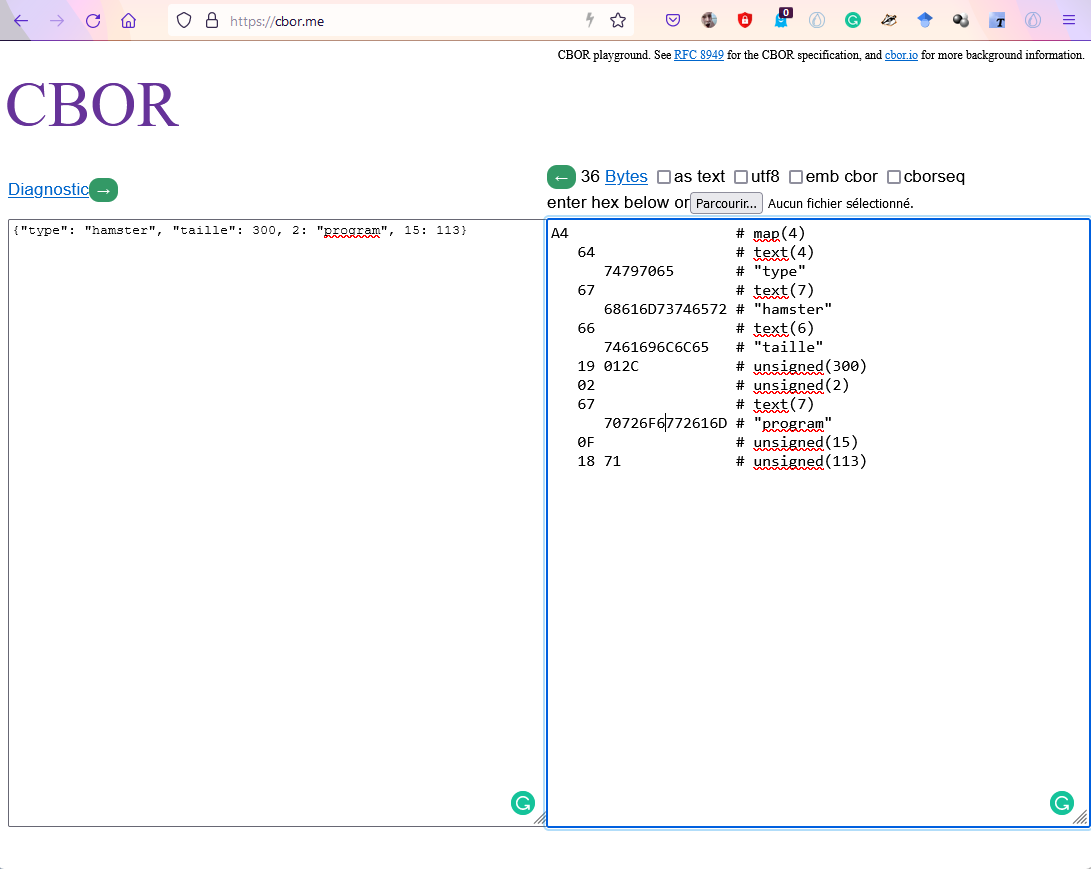
\includegraphics[width=1\columnwidth]{Pictures/cbor-me.png}}
\lgf{\caption{Définition des majeurs en CBOR}}
\lge{\caption{Definition of major in CBOR}}
\label{fig-cbor-me}
\end{figure}

\lgf{Sur ces exemples, on peut voir que CBOR est beaucoup plus permissif et complet que JSON, le premier champ des map CBOR peut être numérique et n'a pas à être unique dans toute la structure. Néanmoins  CBOR
définit un mode strict dans lequel ces clés doivent être codées en ASCII et unique pour être compatibles avec
JSON. Si une clé est répété plusieurs fois dans une structure CBOR, il traiter directement l'information dans la structure CBOR et ne pas chercher à la convertir ou la désérialiser car il y a un risque de perte d'information. }
\lge{On these examples, we can see that CBOR is much more permissive and complete than JSON, the first field of the CBOR map can be numeric and does not have to be unique in the whole structure. Nevertheless CBOR
defines a strict mode in which these keys must be ASCII encoded and unique to be compatible with
JSON. If a key is repeated several times in a CBOR structure, it is necessary to process the information directly in the CBOR structure and not to try to convert or deserialize it because there is a risk of losing information. }


\lgf{\subsection{Type étiquette}}
\lge{\subsection{Type Tag}}


\lgf{CBOR enrichit le typage des données ; ce qui permet de manipuler plus facilement des données. Par exemple, une chaîne de caractères peut représenter une date, une URI, voire une URI codée en base 64. Le type \texttt{110} peut être suivi d'une valeur ou \Index{tag} dont une liste exhaustive est maintenue parl'IANA\footnote{\url{https://www.iana.org/assignments/cbor-tags/cbor-tags.xhtml}}.}
\lge{CBOR enriches the typing of data; this makes it easier to manipulate data. For example, a character string can represent a date, a URI, or even a URI encoded in base 64. The type \texttt{110} can be followed by a value or \Index{tag} of which an exhaustive list is maintained by the IANAfootnote{url{https://www.iana.org/assignments/cbor-tags/cbor-tags.xhtml}}.}

\pythonlst{cbor-tag.py}

\lgf{Par exemple, le programme \pprog{cbor-tag.py}{cbor-example} retourne les résultats suivants~:}
\lge{For example, the program \pprog{cbor-tag.py}{cbor-example} returns the following results:}


\begin{termc}[backgroundcolor=\color{palerod}, language=json, basicstyle=\ttfamily\small, escapechar=@]
# @\textbf{python3.5 cbor-tag.py}@
2018-05-22
c074323031382d30352d32325430303a30303a30305a
2018-05-22 00:00:00+00:00
43010203
<class 'datetime.datetime'>
\end{termc}


\lgf{La représentation canonique montre plus facilement le tag dans la séquence binaire :}
\lge{The canonical representation shows more easily the tag in the binary sequence:}


\begin{termc}[backgroundcolor=\color{palerod}, language=json, basicstyle=\ttfamily\small, escapechar=@]
C0                                      # tag(0)
   74                                   # text(20)
      323031382D30352D32325430303A30303A30305A # "2018-05-22T00:00:00Z"
\end{termc}

\lgf{Le tag 0 implique un format normalisé pour la date ; d'où l'ajout des heures, minutes et secondes, alors qu'elles n'ont pas été spécifiées initialement. On peut également remarquer que \pfunction{cbor2}{loads} retourne un type \texttt{date} et non une chaîne de caractères.}
\lge{The tag 0 implies a normalized format for the date; hence the addition of hours, minutes and seconds, even though they were not initially specified. We can also notice that \pfunction{cbor2}{loads} returns a type \texttt{date} and not a character string.}


\lgf{\subsection{Le type flottant et valeurs particulières}}
\lge{\subsection{The floating type and particular values}}


\lgf{Le dernier type majeur (111) permet de coder les nombres flottants en utilisant la représentation définie par l'\Index{IEEE 754}. Suivant la taille de la représentation, la suite de l'octet contient les valeurs 25 (demi précision sur 16 bits), 26 (simple précision sur 32 bits) ou 27 (double précision sur 64 bits).}
\lge{The last major type (111) allows to encode floating numbers by using the representation defined by the \Index{IEEE 754}. According to the size of the representation, the continuation of the byte contains the values 25 (half precision on 16 bits), 26 (simple precision on 32 bits) or 27 (double precision on 64 bits).}


\lgf{Ce type permet également de coder les valeurs définies par JSON : True (valeur 20), False (valeur 21) ou None (valeur 22).}
\lge{This type also allows to encode the values defined by JSON: True (value 20), False (value 21) or None (value 22).}


\lgf{Finalement, ce type peut indiquer la fin d'un tableau ou d'une liste de paires quand la taille n'est pas connue au début du codage.}
\lge{Finally, this type can indicate the end of an array or a list of pairs when the size is not known at the beginning of the coding.}


\lgf{\section{Questions sur CBOR}}
\lge{\section{Questions about CBOR}}

\Question{\lgf{Avantages de CBOR}\lge{Benefits of CBOR}}
{
\lgf{Quel sont les avantage de CBOR par rapport à JSON (2 réponses) ?}
\lge{What are the advantages of CBOR over JSON (2 answers)?}

\begin{itemize}[label=$\square$]
   \item \Correct{
     \lgf{Il est plus compact dans la représentation des données.}
     \lge{It is more compact in its data representation.}
    }
   \item \Wrong{
    \lgf{Il permet de représenter des nombres flottants.}
    \lge{It allows to represent floating numbers.}
    }
   \item \Wrong{
    \lgf{Il compresse les chaînes de caractères. }
    \lge{It compresses strings. }
    }
   \item \Correct{
    \lgf{Il est plus simple à implémenter.}
    \lge{It is easier to implement.}
    }
 \end{itemize}
   
 }
{
\lgf{CBOR ne compresse pas les chaînes de caractères. Il ajoute juste leur longueur. CBOR et JSON codent tous les deux des nombres flottants, ce n'est donc pas un avantage de CBOR. Par contre, le fait d'utiliser des valeurs binaires au lieu de l'ASCII pour représenter les nombres, de ne pas avoir de crochets ou accolades, permet d'avoir une représentation beaucoup plus compacte. Les petites valeurs numériques sont représentées sans surcoût. Réaliser un codeur ou un décodeur de CBOR est beaucoup plus simple qu'en JSON car la représentation des données est beaucoup plus stricte (pas d'espace, pas de retour à la ligne... ). Les deux représentations permettent d'utiliser des nombres flottant donc aucune n'a d'avantage sur ce point.}
\lge{CBOR does not compress strings. It just adds their length. Both CBOR and JSON encode floating-point numbers, so this is not an advantage of CBOR. On the other hand, using binary values instead of ASCII to represent numbers, not having brackets or braces, makes for a much more compact representation. Small numerical values are represented without any additional cost. Creating a CBOR encoder or decoder is much simpler than in JSON because the data representation is much stricter (no spaces, no line breaks, etc.). Both representations allow to use floating numbers so neither has an advantage on this point.}


}

\Question{\lgf{Flottant}\lge{Floating}}{
\lgf{Un flottant est-il toujours plus compact en CBOR qu'en JSON ? - Vous pouvez vous aider de \url{https://cbor.me}}
\lge{Is a float always more compact in CBOR than in JSON? - You can help yourself with \url{https://cbor.me}}


\begin{itemize}[label=$\circ$]
   \item \Wrong{
    \lgf{Oui, c'est le but de CBOR.}
    \lge{Yes, that is the goal of CBOR.}
    }
   \item \Wrong{
    \lgf{Oui, pour les flottants qui ont la partie décimale à 0.}
    \lge{Yes, for floats that have the decimal part at 0.}
    }
   \item \Wrong{
    \lgf{Oui, pour les flottants de petite précision (jusqu'au centième).}
    \lge{Yes, for small precision floats (up to a hundredth).}
    }
   \item \Correct{
    \lgf{Oui, pour les flottants de grande précision (6 chiffres après la virgule).}
    \lge{Yes, for high precision floats (6 digits after the decimal point).}
    }
 \end{itemize}
}{
\lgf{Un nombre flottant, quelle que soit sa valeur, est représenté par 8 octets en CBOR. En JSON, un nombre flottant est représenté par une chaîne de caractères. Donc "3.0" nécessite 3 caractères, donc plus compacte que CBOR. Mais "3.1415926" est codé sur 9 caractères donc moins compacte que CBOR.}
\lge{A floating number, whatever its value, is represented by 8 bytes in CBOR. In JSON, a floating number is represented by a string. So "3.0" needs 3 characters, so it is more compact than CBOR. But "3.1415926" is coded on 9 characters so less compact than CBOR.}

}

\Question{lgf{Chaîne de caractères}\lgf{Strings}}
{
\lgf{Soit une chaîne de caractères en CBOR.}
\lge{Consider a string in CBOR.}

\begin{itemize}[label=$\circ$]
   \item \Wrong{
    \lgf{Elle est compressée avec un algorithme entropique (e.g. codage de Huffman).}
    \lge{It is compressed with an entropy algorithm (e.g. Huffman coding).}
    }
   \item \Correct{
    \lgf{Elle peut contenir des caractères accentués.}
    \lge{It can contain accented characters.}
    }
   \item \Wrong{
    \lgf{Chaque caractère est codé sur 6 bits.}
    \lge{Each character is coded on 6 bits.}
    }
 \end{itemize}

}{
\lgf{A string is a sequence of bytes. It is possible to use representations offering accented characters (even emoticons). However, CBOR does not compress data.}
}

\Question{\lgf{Taille variable}\lge{Variable length}}
{
\lgf{En CBOR, la taille d'un entier varie en fonction de sa valeur !}
\lge{In CBOR, the size of an integer varies according to its value!}

\begin{itemize}[label=$\circ$]
   \item \Correct{\Vrai}
   \item \Wrong{\Faux}
   \item \Wrong{
    \lgf{Ça dépend de la manière dont on a déclaré cet entier.}
    \lge{It depends on how this integer was declared.}
    }
 \end{itemize}

}{
\lgf{Oui, un entier inférieur à 23 sera codé sur un seul octet. Pour les valeurs plus grandes, il faut ajouter la longueur.}
\lge{Yes, an integer less than 23 will be encoded on a single byte. For larger values, the length must be added.}
}

\Question{\lgf{Tableau}\lge{Array}}
{
\lgf{En CBOR, un tableau peut contenir des objets de types différents.}
\lge{In CBOR, an array can contain objects of different types.}

\begin{itemize}[label=$\circ$]
   \item \Correct{\Vrai}
   \item \Wrong{\Faux}
   \item \Wrong{
   \lgf{Ça dépend de la manière dont on a déclaré ce tableau.}
   \lge{It depends on how this table was declared.}
   }
 \end{itemize}
}
{
\lgf{Vrai, on a la même flexibilité qu'en JSON en imbriquant n'importe quel type de données dans un tableau.}
\lge{True, we have the same flexibility as in JSON by nesting any data type in an array.}
}


\Question{\lgf{Fraction}\lge{Fractional}}
{
\lgf{On veut définir un tableau de deux éléments comme une fraction. Quel tag devra précéder la structure ?
(vous pouvez vous aider du \rfc{8949}).}
\lge{We want to define an array of two elements as a fraction. What tag should precede the structure?
(you can use the \rfc{8949}).}
}
{
\lgf{Il s'agit du tag 4, voir le chapitre \textbf{3.4.4. Decimal Fractions and Bigfloats} du \rfc{8949}.}
\lge{This is tag 4, see the chapter \textbf{3.4.4. Decimal Fractions and Bigfloats} of the \rfc{8949}.}
}

\section{SenML}

\lgf{\ac{SenML} est une une spécification qui exploite JSON ou CBOR. Elle liste un ensemble de noms/unités/mesures et les standardise en un nom de clé unique. En utilisant cette standardisation, on facilite l'interopérabilité. Les clés et valeurs sont donc règlementées et typées pour éviter tous conflits d'interopérabilité. Le format est défini dans la \rfc{8428} et repose sur une structure de tableau regroupant des objets comme le montre la figure suivante tirée de la RFC.}
\lge{\SenML is a specification that leverages JSON or CBOR. It lists a set of names/units/measures and standardizes them into a unique key name. By using this standardization, interoperability is facilitated. The keys and values are therefore regulated and typed to avoid any interoperability conflicts. The format is defined in the RFC{8428} and is based on a table structure grouping objects as shown in the following figure taken from the RFC.}


\begin{termc}[backgroundcolor=\color{palerod}, language=json, basicstyle=\ttfamily\small, escapechar=@]
[
 {"bn" : "urn:dev:ow:10e2073a01080063", "bt":1.320067464e+09,
  "bu" : "\%RH", "v":21.2},
 {"t":10, "v":21.3},
 {"t":20, "v":21.4},
 {"t":30, "v":21.4},
...
\end{termc}

\lgf{SenML définit les clés utilisées dans l’objet. Pour avoir une notation compacte, elles sont limitées à 1 ou 2 caractères. Parmi elles, ”bn” indique un nom de base et ”n” le nom d’un appareil. Si plusieurs appareils envoient la partie commune de l’identifiant de l’appareil, on peut mettre le ”bn” pour éviter de le répéter à chaque fois.}
\lge{SenML defines the keys used in the object. To have a compact notation, they are limited to 1 or 2 characters. Among them, "bn" indicates a base name and "n" the name of a device. If several devices send the common part of the device identifier, we can put the "bn" to avoid repeating it each time.}

\lgf{Le temps de base (ou ”bt”) est également un moyen de compacter la notation du temps. Le temps (”t”) donne le décalage et conduit à une valeur plus petite comme on le voit dans l’exemple.}
\lge{The base time (or "bt") is also a way to compact the time notation. The time ("t") gives the offset and leads to a smaller value as seen in the example.}


\lgf{L’unité de base (”bu”) indique l’unité par défaut si les autres objets ne portent pas de mot clé indiquant l’unité (”u”).}
\lge{The base unit ("bu") indicates the default unit if the other objects do not have a keyword indicating the unit ("u").}

\lgf{La \rfc{8428} définit une liste d’unités telles que le kilogramme (”kg”), le volt (”V”), etc. Dans l’exemple, ”\%RH” désigne un pourcentage d’humidité relative. Une valeur numérique utilise la lettre ”v”, une chaîne de caractères utilise la touche ”vs”.}
\lge{The \rfc{8428} defines a list of units such as kilogram ("kg"), volt ("V"), etc. In the example, "\%RH" refers to a percentage of relative humidity. A numeric value uses the letter "v", a string uses the "vs" key.}


\lgf{CBOR utilise la même structure mais les petits nombres entiers positifs et négatifs sont substitués dans les clés des objets de CBOR : ”bn”, ”bt”, ”bu” seront respectivement représentés par -1, -2 et -3 et ”n”, ”t”, ”u” par +0, +2 et +6.}
\lge{CBOR uses the same structure but small positive and negative integers are substituted in the keys of CBOR objects: "bn", "bt", "bu" will be represented by -1, -2 and -3 respectively and "n", "t", "u" by +0, +2 and +6.}



\cleardoublepage

\chapter{Mettre en œuvre un Capteur Virtuel}

\textit{Les programmes relatifs à cette section se trouvent dans le répertoire \texttt{plido-tp3}. Il est recommandé d'utiliser la machine virtuelle avec une fenêtre de terminal pour l'objet et une autre pour le serveur.}

\section {JSON}

\begin{wrapfigure}{r}{3cm}
\Youtube{https://youtu.be/mRuEiwa7Z74}
\end{wrapfigure}

Ca fait longtemps qu'on parle d'Internet des Objets, il est temps de mettre en pratique nos connaissances. On va commencer par une mise en oeuvre simple en Python sur votre machine. Le but dans cette partie est de tester tout ce qu'on a vu sans autre matériel qu'un ordinateur. Nous allons ouvrir deux fenêtres terminal. Dans l'une nous allons faire tourner un programme qui va émuler l'objet avec trois capteurs. Cet objet va communiquer avec un serveur qui va recueillir l'information. La communication se fera en interne avec une socket utilisant l'interface \Index{loopback} (cf. figure~\vref{fig-deux-terminaux}).


\begin{figure}[tbp]
\centerline{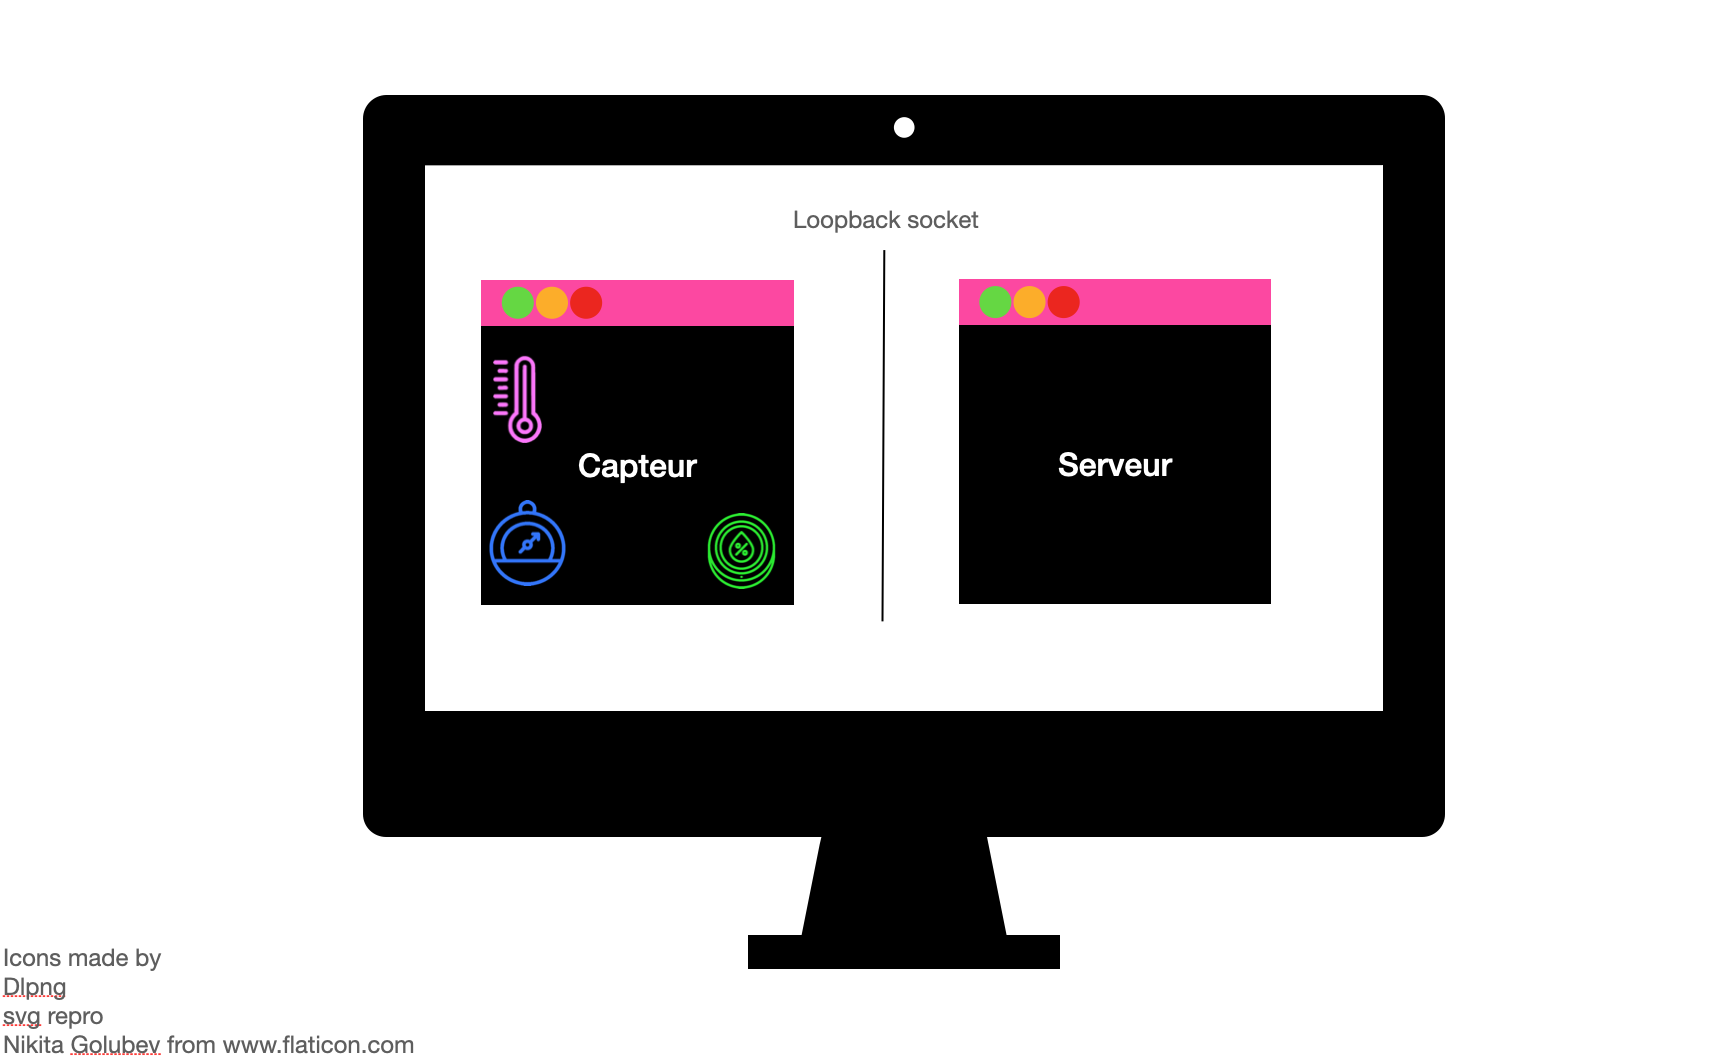
\includegraphics[width=1\columnwidth]{Pictures/Capture24.png}}
\caption{Architecture client serveur}
\label{fig-deux-terminaux}
\end{figure}

\subsection{Serveur Minimal}\label{chap-mini-serv}

\pythonlst{minimal\_server.py}


Commençons par construire un serveur sommaire (\texttt{minimal\_server.py}) qui va afficher tout ce qu'il reçoit. 
\begin{itemize}
    \item lignes 1 et 2 les modules \texttt{socket} pour la communication et \texttt{binascii} pour transformer le binaire en chaîne de caractères.
    \item ligne 4, la \pfunction{socket}{socket} crée la socket \texttt{s} avec les paramètres pour des communications IP (\texttt{AF\_INET}) et UDP (\texttt{SOCK\_DGRAM}).
    \item ligne 5, la socket est associée au numéro de port \texttt{33033} via la fonction \pfunction{socket}{bind}. L'adresse \texttt{0.0.0.0} indique que les données peuvent venir de n'importe quelle interface (Ethernet, Wi-Fi, loopback,...) 
    \item ligne 8, dans la boucle sans fin, la fonction \pfunction{socket}{recvfrom} va se bloquer dans l'attente de données. Elle retourne les données et l'adresse de l'émetteur.
    \item ligne 9, les données sont affichées en chaîne d'octets et en hexadécimal.
    
\end{itemize}

     \vspace{1em}

On lance le programme serveur. Comme personne lui parle, il n'affiche rien. 

\subsection{Capteur virtuel}

\pythonlst{virtual\_sensor.py}

Le module \Index{virtual\_sensor} avec la classe du même nom, reflète de manière à peu près réaliste le comportement d'un capteur. On voit dans le programme principal (ligne 23 à 37) que l'on créé trois capteurs virtuels : un pour la température (ligne 31), un autre pour la pression (ligne 32), et le troisième pour l'humidité (ligne 34). L'argument \texttt{start} précise la valeur de départ, \texttt{variation} la plage de variation entre deux mesures et \texttt{min} et \texttt{max} les valeurs à ne pas dépasser. La boucle sans fin qui affiche les différentes valeurs toutes les secondes.

\begin{termc}[backgroundcolor=\color{palerod}, language=json, basicstyle=\ttfamily\small, escapechar=@]
> @\textbf{python3 virtual\_sensor.py}@
 54.956    999.850  30.609
 54.963   1000.473  32.505
 55.062   1000.845  31.870
 55.017   1001.619  32.257
 55.083   1000.767  31.757
 55.027   1001.442  31.742
 \end{termc} 

\subsubsection{Envoi direct}

\pythonlst{minimal\_client1.py}
Des scripts utilisant ce module peuvent être écrit, comme par exemple le programme \texttt{minimal\_client1.py}.

La variable \texttt{t} contient la température qui est émise sur le port 33033 à l’adresse de \textit{loopback}. On obtient ainsi une communication entre deux programmes dans votre ordinateur dont l'adresse IP locale est \texttt{127.0.0.1}. Mais quand on lance le programme \texttt{minimal\_client1.py}, on obtient l’erreur suivante :

\begin{termc}[backgroundcolor=\color{palerod}, language=json, basicstyle=\ttfamily\small, escapechar=@]
 >python3.5 minimal_client1.py
Traceback (most recent call last):
  File "minimal_client1.py", line 11, in <module>
    s.sendto (t, ("127.0.0.1", 33033))
TypeError: a bytes-like object is required, not 'float'
\end{termc}

\Question{Bug ?}
{Pourquoi le programme client ne fonctionne pas ?
\begin{itemize}[label=$\circ$]
   \item \Wrong{L’adresse IP n’est pas correcte.}
   \item \Correct{Il manque un processus de sérialisation de la donné}
   \item \Wrong{La variable \texttt{t} n’est pas définie}
   \item \Wrong{La variable \texttt{t} ne peux pas être lue.}
 \end{itemize}
}
{La variable \texttt{t} pointe vers une représentation en mémoire du nombre flottant. Elle ne peut pas être directement envoyée à un autre équipement. Il faut ajouter une phase de sérialisation qui va permettre de transmettre cette information soit en une chaîne de caractères, soit en une chaîne d'octets.}

\subsubsection{Envoi d'une chaîne d'octets}

\pythonlst[firstline=9,lastline=11, firstnumber=9]{minimal\_client2.py}

Dans le programme \texttt{minimal\_client2.py}, le nombre flottant contenu dans la variable \texttt{t} est transformé en chaîne de caractères avec la fonction \texttt{\Index{str}}, puis en chaîne d'octets avec la méthode \pfunction{str}{encode} pour être compatible avec l'argument attendu par la méthode \pfunction{socket}{sendto}. Coté serveur la fonction \texttt{\Index{str}} converti la chaîne d'octets reçue en flottant.

\subsubsection{Envoi de plusieurs valeurs}

\pythonlst[firstline=11,lastline=17, firstnumber=11]{minimal\_client3.py} % 

Pour envoyer simultanément les valeurs des trois capteurs, la représentation via une chaîne de caractères est un peu plus compliquée à mettre en oeuvre. Si le programme \texttt{minimal\_client3.py} utilise \pfunction{str}{format} pour envoyer des données séparées par des vigules. Côté serveur, il faut décoder cette chaîne pour y retrouver les entiers. Et ça c'est beaucoup plus complexe à faire ! 

\subsubsection{JSON}

\pythonlst[firstline=12,lastline=19, firstnumber=12]{minimal\_client4.py} %

La solution la plus simple est de mettre ces trois valeurs dans un tableau python et de le transformer en une représentation JSON grâce à la fonction \pfunction{json}{dumps} du module \texttt{json}. 

     \vspace{1em}

Cette chaîne de caractères JSON est à son tour transformé en chaîne d'octets avec encode et envoyée au serveur. Dans notre cas, le serveur ne fait qu'afficher la chaîne de caractères mais vous pouvez utiliser la méthode \pfunction{json}{loads} du module \texttt{json} pour desérialiser et en faire une structure Python dans le serveur, sur laquelle il est maintenant facile d'effectuer des opérations comme, par exemple, un calcul de moyenne.

\begin{termc}[backgroundcolor=\color{palerod}, language=json, basicstyle=\ttfamily\tiny, escapechar=@]
% @\textbf{python3 minimal\_server.py}@
b'[19.93044784157464, 999.1552628155773, 35.723583473834566]' => b'5b31392e39333034343738343135373436342c203939392e313535c...
b'[19.940155545405723, 998.7581534530281, 35.820037116376184]' => b'5b31392e3934303135353534353430353732332c203939382e3735...
b'[20.003803212269627, 999.3517302791449, 34.33544522779677]' => b'5b32302e3030333830333231323236393632372c203939392e33353...
\end{termc}

\section{CBOR}

\begin{wrapfigure}{r}{3cm}
\Youtube{https://youtu.be/PmudahiRWFw}
\end{wrapfigure}

Le passage de JSON à CBOR est très simple. Il suffit de changer un module \texttt{cbor} à la place du module de \texttt{json}. Le programme \texttt{minimal\_client5.py}~:
\begin{itemize}
    \item ligne 1 fait appel au module cbor2 en le renommant cbor
    \item le reste du programme est identique au précédent, ce n'est que dans la la sérialisation, ligne 18, que la fonction \texttt{json.\pfunction{json}{dumps}} est remplacée par \texttt{cbor.\pfunction{cbor2}{dumps}}. Le format retourné étant une chaîne d'octets, il n'est plus nécessaire de faire appel à la méthode \texttt{encode}.
\end{itemize}


     \vspace{1em}


Le programme \pprog{minimal\_server.py}{plido-tp3} n'est pas modifié puisqu'il ne fait qu'afficher ce qu'il reçoit. 







\begin{termc}[backgroundcolor=\color{palerod}, language=json, basicstyle=\ttfamily\small, escapechar=#]
> #\texttbf{python3 minimal\_server.py}#
b'\x83... => b'83fb40341086f3e8b66bfb408f3b7791c8d61ffb403fac15ba06088e'
b'\x83... => b'83fb40341d4d28495268fb408f33d502185c3dfb403d95a2c4981444'
\end{termc}


\pythonlst{minimal\_client5.py}

On obtient le résultat suivant. La séquence CBOR fait 28 octets de long, l'équivalant JSON aurait fait 60 octets. Même si cela divise par deux la taille des données à transmettre, le résultat n'est pas compact. Cela tient à la représentation des nombres flottants en CBOR, car ici les flottant sont codés sur 8 octets.

\Question{Décodage}{
Analysons la séquence reçue: \texttt{83fb40341086f3e8b66bfb408f3b7791c8d61ffb403fac 15ba06088e}

À quoi correspond l’octet 0x83 qui commence la structure CBOR reçue ?
\begin{itemize}[label=$\circ$]
   \item \Wrong{au codage de l'entier positif 131 .}
   \item \Wrong{au codage de l'entier négatif 132 .}
   \item \Correct{à la définition d'un tableau de 3 éléments.́}
   \item \Wrong{à la définition d'un map CBOR de 3 éléments}
   \item \Wrong{à la définition d'un tableau de taille non définie.}
 \end{itemize}
 }
 {
 0x83 s'écrit en binaire \texttt{100-0 0111}. \texttt{100} est le type majeur pour un tableau. La valeur \texttt{00111} est inférieure à 24. Il s'agit donc du nombre d'éléments du tableau, donc un tableau de 3 éléments.
 }

\Question{Flottant}
{Dans cette chaîne, uel est le marqueur CBOR (en hexadécimal) qui indique que l’on a un nombre flottant ?}
{0xFB, si on l'écrit en binaire on obtient \texttt{111-1 1100}. Le majeur correspond à la catégorie des flottant et des valeurs spéciales.}

\Question{Taille du flottant}
{Quelle est la taille de ce flottant en octets ?}
{8 octets~; la partie mineur \texttt{1 1100} indique qu'il s'agit d'un flottant codé sur 8 octets}

\subsubsection{Utilisation de nombres entiers}

Pour réduire la taille des données transmises, nous allons utiliser des nombres entiers. Nous aurons besoin d’une précision au centième (deux chiffres après la virgule). Pour ce faire, il suffit, du coté du client, de prendre la partie entière du nombre multiplié par 100 et, du côté du serveur, de diviser la valeur reçue par 100. La modification du code est mineure.

\pythonlst[firstline=17,lastline=18, firstnumber=17]{minimal\_client6.py}


\begin{termc}[backgroundcolor=\color{palerod}, language=json, basicstyle=\ttfamily\tiny, escapechar=#]
> #\texttbf{python3 minimal\_server.py}#
b'\x83\x19\x07\xd7\x1a\x00\x01\x86O\x19\x0c\xa7' => b'831907d71a0001864f190ca7'
b'\x83\x19\x07\xd4\x1a\x00\x01\x86f\x19\x0cJ' => b'831907d41a00018666190c4a'
b'\x83\x19\x07\xd4\x1a\x00\x01\x86\x92\x19\rP' => b'831907d41a00018692190d50'
\end{termc}

La modification est mineure et tient en 12 octets, mais il y a une diminution au niveau de l'interopérabilité, car les deux entités doivent connaître la transformation de la valeur liée à la multiplication par 100.

\Question{Anticipons la taille}
{ Quelle est la taille minimale et maximale de la structure CBOR envoyée, en prenant en compte les valeurs possibles.
}
{
\begin{itemize}
    \item La température peut évoluer raisonnablement entre -30 et +50, soit -3000 et +5000 après la transformation en entier. La taille minimale, si on envoie 0, la taille sera d'un octet. La taille maximale tiennent sur 3 octets (1 pour le type/longueur et 2 pour les valeurs) 
    \item La pression évolue autour de 1000, soit 100~000 après la transformation en entier. La taille sera toujours de 5 octets (1 pour le type/longueur, 4 pour les valeurs)
    \item Le taux d'humidité évolue entre 0 et 100 , soit 0 et 10 000 après la transformation en entier. L a taille entre 1 octet et 3 octets
\end{itemize}

Si on ajoute le type/longueur 0x83 pour indiquer un tableau de trois éléments, on obtient une taille minimale de 1+1+5+1= 8 octets et une taille maximale de 1+3+5+3 = 12 octets.
}

\cleardoublepage

\lgf{\chapter{Séries temporelles}}
\lge{\chapter{Time series}}


\begin{wrapfigure}{r}{3cm}
\Youtube{https://youtu.be/xrdCY4iN40s}
\end{wrapfigure}

\lgf{Les capteurs virtuels que nous avons programmés jusqu’à présent émettent les données à chaque fois que celles-ci sont mesurées. 
Cela permet au serveur de suivre en temps réel le comportement du système étudié. 
Mais dans certains cas, le temps réel n’est pas nécessaire et il est préférable de limiter le nombre d’émissions, par exemple pour économiser l'énergie du capteur.}
\lge{The virtual sensors that we have programmed so far emit data each time they have a measurement. 
This allows the server to follow the behavior of the studied system in real time. 
But in some cases, real time is not necessary and it is preferable to limit the number of emissions, for example to save the energy of the sensor.}

\lgf{Pour ce faire, nous pouvons utiliser un tableau qui va accumuler les valeurs et l’envoyer quand le tableau atteint une certaine taille.}
\lge{To do this, we can use an array that will accumulate the values and send it when the array reaches a certain size.}


\lgf{\section{Envoi d'un tableau}}
\lge{\section{Sending an array}}


\lgf{Le programme \pprog{minimal\_humidity1.py}{plido-tp3} accumule les données dans un tableau \texttt{h\_humidity} quand celui-ci atteint 30 éléments (ligne 17), les données sont envoyées au serveur.}
\lge{The program \pprog{minimal\_humidity1.py}{plido-tp3} accumulates the data in an array \texttt{humidity} when this one reaches 30 elements (line 17), the data are sent to the server.}

\pythonlst{minimal\_humidity1.py}



\begin{termc}[backgroundcolor=\color{palerod}, basicstyle=\ttfamily\small, escapechar=\#]
1 4 [3241]
2 7 [3241, 2945]
3 10 [3241, 2945, 2762]
4 13 [3241, 2945, 2762, 2625]
5 16 [3241, 2945, 2762, 2625, 2480]
6 19 [3241, 2945, 2762, 2625, 2480, 2769]
\end{termc}

\lgf{Le premier chiffre de la ligne indique le nombre d'éléments et le second la taille dans le codage CBOR. On remarque que l'ajout d'un élément augmente la taille du tableau de 3 octets. Les valeurs correspondant à une mesure d'humidité ne varient pas fortement. Ainsi un tableau de 30 mesures a une taille de 92 octets.}
\lge{The first digit of the line indicates the number of elements and the second the size in the CBOR coding. We notice that adding an element increases the size of the array by 3 bytes. The values corresponding to a moisture measurement do not vary greatly. Thus an array of 30 measurements has a size of 92 bytes.}

\lgf{\section{Codage par différence}}
\lge{\section{Differential coding}}

\lgf{On peut optimiser le volume de données transférées en utilisant un codage par delta (i.e. la variation de l'humidité). 
La première valeur du tableau correspond à la valeur mesurée tandis que les suivantes représentent la différence entre la valeur mesurée et la précédente.}
\lge{The amount of data transferred can be optimized by using delta coding (i.e. the variation in humidity). 
The first value in the table is the measured value while the following values represent the difference between the measured value and the previous one.}

\pythonlst[firstline=17,lastline=26,  firstnumber=17]{minimal\_humidity2.py}%[firstline=282,lastline=19, firstnumber=282]

\lgf{Le programme \pprog{minimal\_humidity2.py}{plido-tp3} gère différemment le remplissage du tableau~:}
\lge{The program \pprog{minimal\_humidity2.py}{plido-tp3} handles the filling of the array differently:}

\begin{itemize}
    \item 
        \lgf{ligne 14 et 15, si le tableau est vide, le tableau est créé avec la valeur mesurée,}
        \lge{line 14 and 15, if the table is empty, the table is created with the measured value,}
    \item 
        \lgf{ligne 16 à 22, sinon si le tableau est plein, il est sérialisé en CBOR et envoyé au serveur, puis réinitialisé avec la valeur mesurée,}
        \lge{line 16 to 22, otherwise if the table is full, it is serialized in CBOR and sent to the server, then reset with the measured value,}
    \item 
        \lgf{ligne 23 et 24, sinon la différence entre la précédente valeur et celle mesurée est stockée dans le tableau.}
        \lge{line 23 and 24, otherwise the difference between the previous value and the measured value is stored in the table.}
\end{itemize}

       \vspace{1em}

\lgf{Le listing suivant donne un exemple d'exécution.}
\lge{The following listing gives an example of execution.}


\begin{termc}[backgroundcolor=\color{palerod}, basicstyle=\ttfamily\small, escapechar=\#]
1 4 [2521]
2 6 [2521, 79]
3 8 [2521, 79, 224]
4 10 [2521, 79, 224, -40]
5 12 [2521, 79, 224, -40, -112]
6 13 [2521, 79, 224, -40, -112, 1]
7 15 [2521, 79, 224, -40, -112, 1, 130]
8 18 [2521, 79, 224, -40, -112, 1, 130, -288]
9 21 [2521, 79, 224, -40, -112, 1, 130, -288, 299]
\end{termc}

\lgf{Ceci met en valeur deux souplesses de CBOR~:}
\lge{This highlights two flexibilities of CBOR:}
\begin{itemize}
    \item 
        \lgf{la taille du tableau est dynamique. Si l’on change le nombre de valeurs à transmettre, le tableau l’indique et l’on n’a pas besoin de modifier le code du récepteur~;}
        \lge{the size of the table is dynamic. If the number of values to be transmitted is changed, the array indicates this and there is no need to modify the receiver code;}
    \item 
        \lgf{la taille des données dépend de leur valeur. 
        Pour les variations entre -24 et +23, un seul octet sera nécessaire. 
        On le voit sur l’exemple précédent : l’ajout de la valeur '1' dans le tableau fait passer la taille de la représentation CBOR de 12 à 135 octets. Les valeurs entre 256 et +255 sont transmises sur 2 octets ; il est donc possible de cette manière d’optimiser la transmission sans ajouter de contrainte. S’il y avait une brusque variation de l’humidité, la représentation CBOR s’adapterait pour la transmettre.}
        \lge{the size of the data depends on its value. 
        For variations between -24 and +23, only one byte will be necessary. 
        We can see it on the previous example: the addition of the value '1' in the table increases the size of the CBOR representation from 12 to 135 bytes. The values between 256 and +255 are transmitted on 2 bytes; it is thus possible in this way to optimize the transmission without adding constraints. If there was a sudden change in humidity, the CBOR representation would adapt to transmit it.}
        
\end{itemize}

\lgf{La taille est réduite d"un tiers (environ 66 octets) pour transmettre la même information.}
\lge{The size is reduced by one third (about 66 bytes) to transmit the same information.}

\section{Architecture}

\lgf{La figure~\vref{fig-client-serveur} représente l'architecture générale du système. Le programme \pprog{minimal\_humidity2.py}{plido-tp3} fournit les séries temporelles. Il reste à définir le programme serveur qui va les traiter et faire appel à un autre service pour les afficher sous forme de graphe. }
\lge{Figure~\vref{fig-client-server} represents the general architecture of the system. The program \pprog{minimal_humidity2.py}{plido-tp3} provides the time series. It remains to define the server program which will process them and call another service to display them in the form of a graph. }


       \vspace{1em}


\lgf{Si l'on suit le flux d'information, le capteur va produire des données au format CBOR pour être compact et le programme serveur va transformer cette information en une structure JSON respectant les spécifications du service d'affichage.}
\lge{If we follow the information flow, the sensor will produce data in CBOR format to be compacted and the server program will transform this information into a JSON structure respecting the specifications of the display service.}

\begin{figure}[tbp]
\centerline{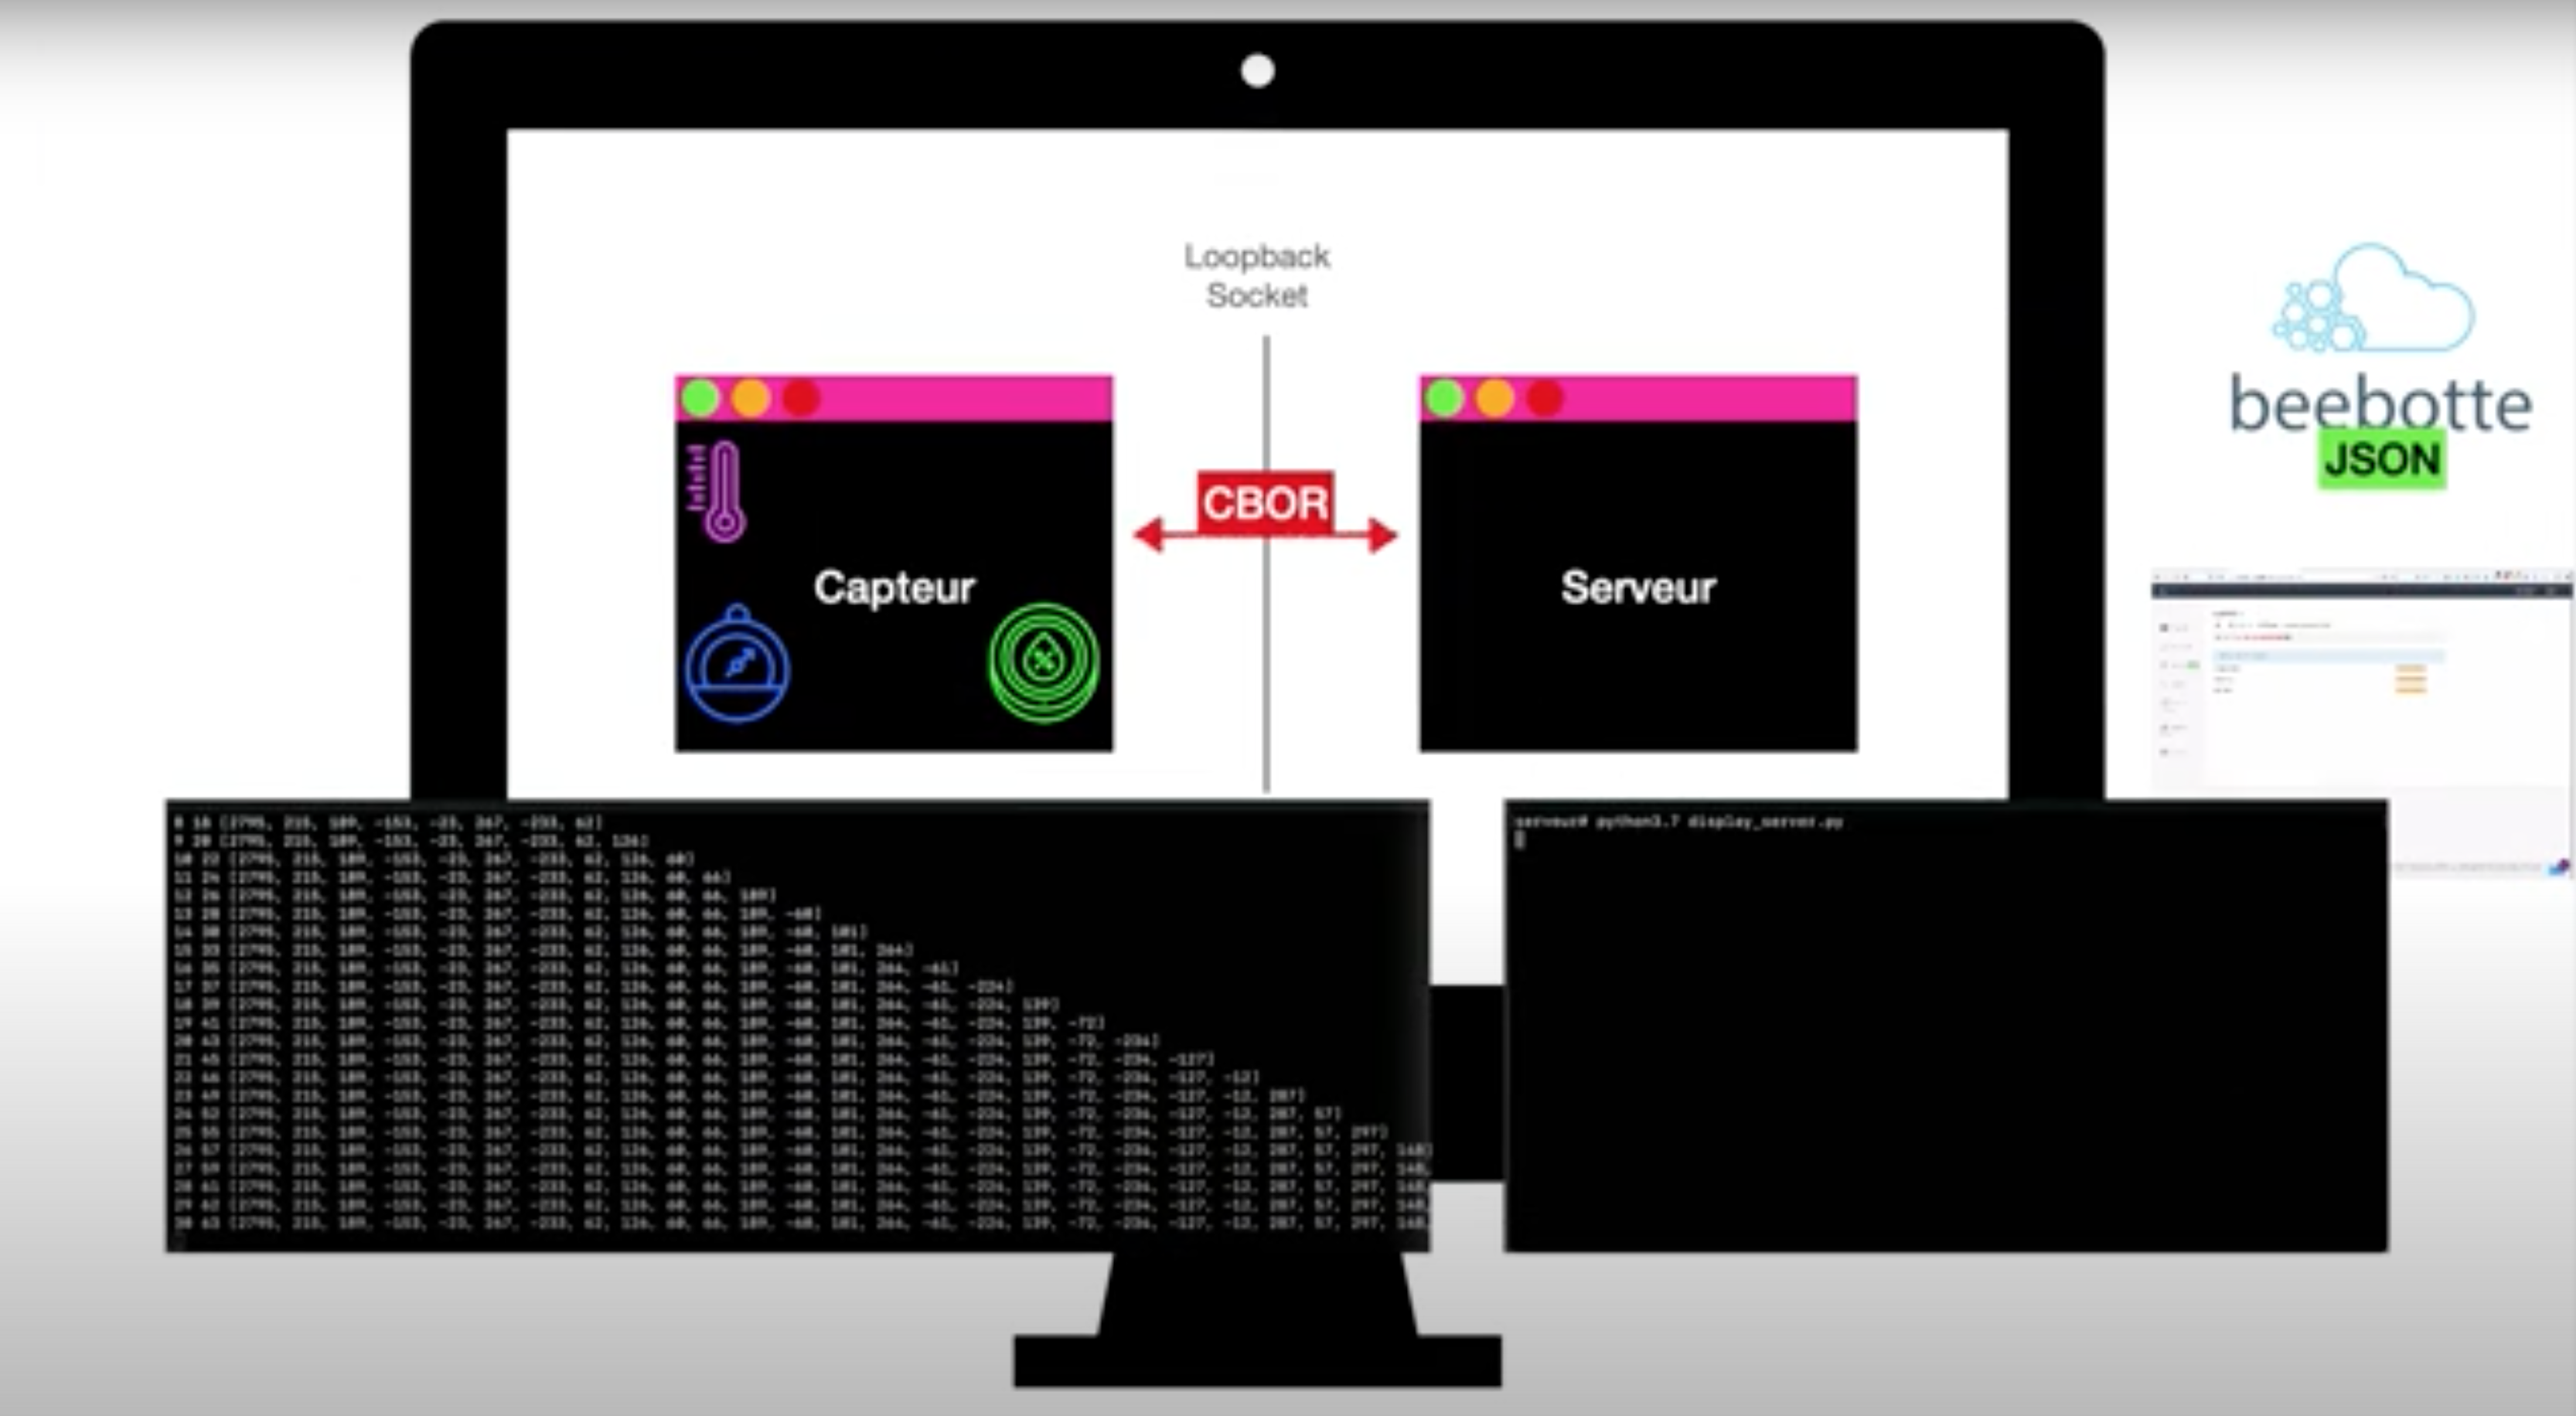
\includegraphics[width=1\columnwidth]{Pictures/Capture40.png}}
\lgf{\caption{Architecture Client/Serveur}}
\lge{\caption{Client/Server Architecture}}
\label{fig-client-serveur}
\end{figure}

\section{\Index{Beebotte}}

\lgf{Il existe plusieurs sites qui permettent de le faire. Nous allons utiliser \url{https://beebotte.com}, mais ce que nous allons présenter peut très bien s'appliquer à d'autres sites.}
\lge{There are several sites that allow you to do this. We are going to use \url{https://beebotte.com}, but what we are going to present can very well be applied to other sites.}

\subsection{Configuration}

\begin{wrapfigure}{r}{3cm}

\includegraphics[width=.2\columnwidth]{Pictures/beebotte.png}
\end{wrapfigure}

\lgf{La première étape consiste à créer un compte en cliquant sur \textit{Sign Up} sur la page de garde et en remplissant un formulaire classique avec votre login, adresse de courrier électronique et mot de passe. Une fois le compte validé, le service est accessible.}
\lge{The first step is to create an account by clicking on \textit{Sign Up} on the front page and filling out a standard form with your login, email address and password. Once the account is validated, the service is accessible.}


\lgf{Le compte nous permet de nous authentifier pour gérer les données sur le site, mais il faut également disposer d’autorisation pour pouvoir y déposer des données via l’\Index{API REST}.
Pour cela, il faut se rendre sur la page \textit{Account Setting} puis l’onglet \textit{Access Management}. 
Cette page (cf. figure~\vref{fig-bb-key}) donne une clé et un secret pour gérer l’ensemble des données sur le site. }
\lge{The account allows us to authenticate ourselves to manage the data on the site, but we also need to have authorization to be able to deposit data via the \Index{API REST}.
To do this, you must go to the \textit{Account Setting} page and then the \textit{Access Management} tab. 
This page (see figure~\vref{fig-bb-key}) gives a key and a secret to manage all the data on the site. }


\begin{figure}[tbp]
\centerline{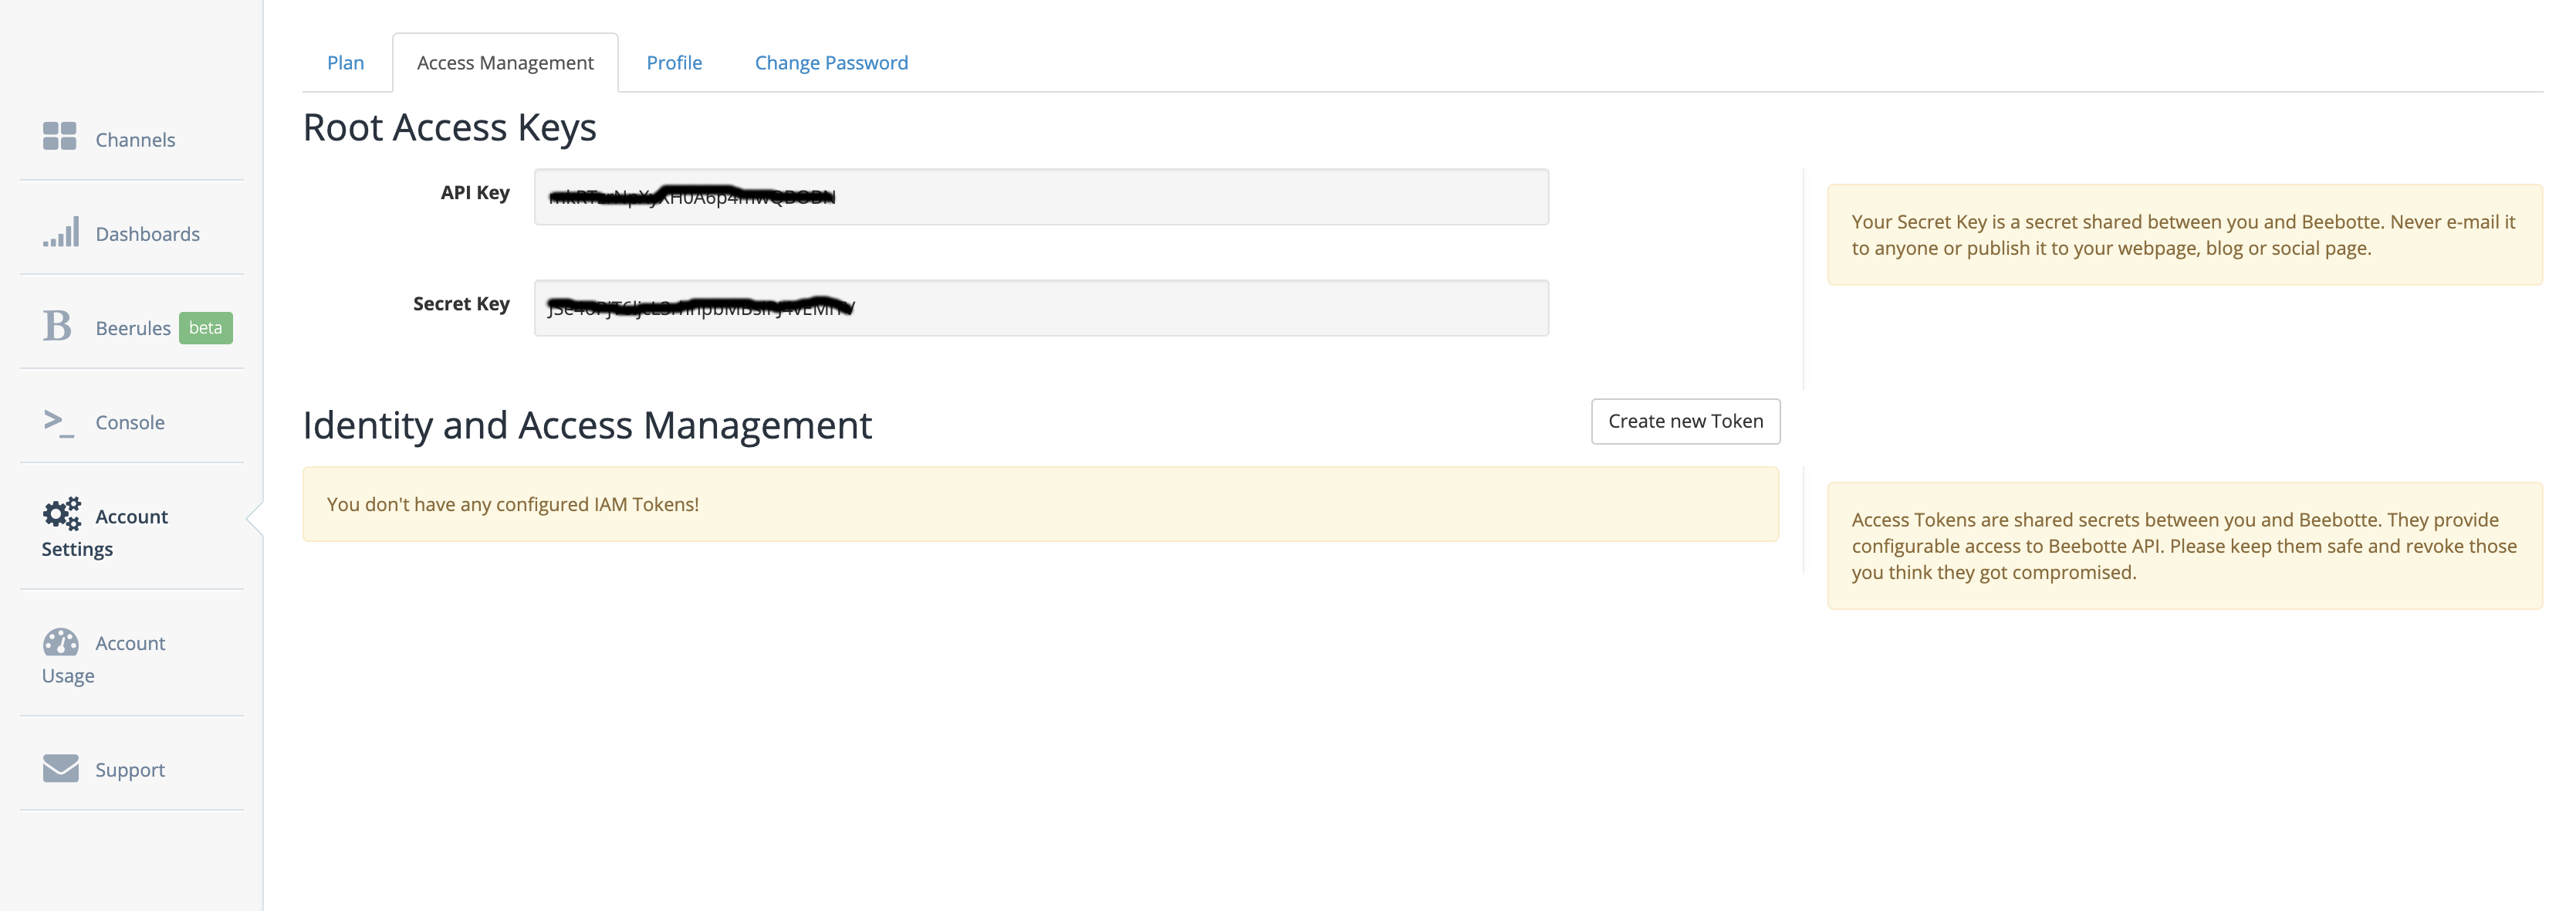
\includegraphics[width=1\columnwidth]{Pictures/bb_root_token.png}}
\lgf{\caption{Clé et secret pour l'authentification}}
\lge{\caption{Key and secret for authentication}}
\label{fig-bb-key}
\end{figure}

\lgf{Notez ces valeurs et stockez les dans un fichier \pprog{config\_bbt.py}{plido-tp3} qui a cet aspect (vos valeurs sont forcément différentes)~:}
\lge{Note these values and store them in a file called \pprog{config\_bbt.py}{plido-tp3} that looks like this (your values are bound to be different):}

\pythonlst{config\_bbt.py}

\lgf{Nous allons maintenant créer un canal (\textit{channel}) dans lequel nous allons définir les objets correspondant aux capteurs. En Cliquant sur \textit {Channels} puis \textit{Create New}, la page représentée figure~\vref{fig-new-channel} apparaît. }
\lge{We are now going to create a channel (\textit{channel}) in which we will define the objects corresponding to the sensors. By clicking on \textit{Channels} and then \textit{Create New}, the page shown in figure~ref{fig-new-channel} appears. }

\lgf{Il faut donner un nom au channel (\textit{capteurs} dans l'exemple), cocher la case \textit{public} et créer trois ressources pour les trois valeurs qui nous intéressent (\textit{temperature}, \textit{humidity}, \textit{presure}) et faire correspondre les unités.}
\lge{You have to give a name to the channel (\textit{sensors} in the example), check the \textit{public} box and create three resources for the three values we are interested in (\textit{temperature}, \textit{humidity}, \textit{presure}) and match the units.}

\lgf{\subsection{Enregistrement des ressources}}
\lge{\subsection{Resource registration}}

\lgf{Le programme \pprog{display\_server.py}{plido-tp3} permet de correspondre avec Beebotte via son API REST. Il commence par l'importation des modules nécessaires~:}
\lge{The program \pprog{display\_server.py}{plido-tp3} allows to correspond with Beebotte via its REST API. It starts by importing the necessary modules:}



\pythonlst[firstline=1,lastline=8, firstnumber=1]{display\_server.py}


\begin{itemize}
    \item 
        \lgf{ligne 4, le module Python \texttt{beebotte}  est disponible pour simplifier la manipulation des données\footnote{S'il n'était pas présent sur votre ordinateur, vous devriez l'installer avec la commande \texttt{pip3 install beebotte}.}.}
        \lge{line 4, the Python module \texttt{beebotte} is available to simplify the manipulation of data\footnote{If it was not present on your computer, you should install it with the command \texttt{pip3 install beebotte}.}.}
    \item 
        \lgf{ligne 5, le module \texttt{contient} la clé et le secret nécessaire à la connexion obtenu précédemment.}
        \lge{line 5, the module \texttt{contains} the key and the secret necessary to the connection obtained previously.}
    
\end{itemize}

\pythonnxt[firstline=9,lastline=11, firstnumber=9]{display\_server.py}

\begin{itemize}
    \item 
        \lgf{ligne 10 et 11 permette d'ouvrir la socket pour communiquer avec les capteurs.}
        \lge{line 10 and 11 allow to open the socket to communicate with the sensors.}
\end{itemize}

\pythonnxt[firstline=12,lastline=14, firstnumber=12]{display\_server.py}

\begin{itemize}
    \item 
        \lgf{ligne 13 une instance permettant la connexion avec les serveurs de Beebotte est définie grâce à la fonction \pfunction{beebotte}{BBT}. Les paramètres de connexion provenant du module \texttt{config\_bbt} sont pris en compte. }
        \lge{line 13 an instance allowing the connection with the Beebotte servers is defined thanks to the function \pfunction{beebotte}{BBT}. The connection parameters from the module \texttt{config\_bbt} are taken into account. }
\end{itemize}

\pythonnxt[firstline=41,lastline=45, firstnumber=41]{display\_server.py}

\lgf{Dans le programme principal, un boucle sans fin attend la série temporelle codée en CBOR venant du capteur (ligne 42), les transforme tableau Python (ligne 44) et appelle la fonction \texttt{to\_btt} en précisant~:}
\lge{In the main program, an endless loop waits for the CBOR coded time series coming from the sensor (line 42), transforms them into a Python array (line 44) and calls the function \texttt{to\_btt} by specifying:}
\begin{itemize}
    \item 
        \lgf{le canal et la ressource qui ont été définie précédemment sur Beebotte~;}
        \lge{the channel and resource that were previously defined on Beebotte;}
    \item 
        \lgf{la série temporelle~;}
        \lge{the time series;}
    \item 
        \lgf{la précision pour transformer ces entiers en flottant.}
        \lge{the precision to transform these integers into floats.}
\end{itemize}

\pythonnxt[firstline=15,lastline=38, firstnumber=15]{display\_server.py}

\lgf{La fonction \texttt{to\_bbt} fait l’essentiel du travail de transformation. Elle prend en argument~:}
\lge{The function \texttt{to\_bbt} does most of the transformation work. It takes as argument:}

\begin{itemize}
    \item 
        \lgf{le nom du canal créé sur Beebotte. Dans notre cas, ce sera \texttt{capteurs}~;}
        \lge{the name of the channel created on Beebotte. In our case, it will be \texttt{sensors};}
    \item  
        \lgf{le nom de l’objet dans ce canal que nous avons également créé sur le site web. Dans notre cas, ce sera \texttt{humidity}~;}
        \lge{the name of the object in this channel that we have also created on the website. In our case, it will be \texttt{humidity};}
    \item  
        \lgf{le tableau Python des mesures codées en delta~;}
        \lge{the Python table of delta-coded measurements;}
    \item  
        \lgf{le facteur multiplicatif, c’est-à-dire la précision. Ici, il faudra diviser par 100~;}
        \lge{the multiplicative factor, i.e. the precision. Here, you will have to divide by 100;}
    \item  
        \lgf{la période entre deux mesures ; cela nous permettra de calculer l’instant de la mesure. Par défaut, la période est de 10 secondes~;}
        \lge{the period between two measurements; this will allow us to calculate the time of the measurement. By default, the period is 10 seconds;}
    \item  
        \lgf{le temps de réception du message pour dater les échantillons. S’il n’est pas spécifié, le temps courant est pris.}
        \lge{the time of reception of the message to date the samples. If it is not specified, the current time is taken.}

\end{itemize}

       \vspace{1em}

\lgf{Cette fonction transforme le tableau Python suivant~:}
\lge{This function transforms the following Python table:}


\begin{termc}[backgroundcolor=\color{palerod},  basicstyle=\ttfamily\small, escapechar=\#]
[3311, 124, -144, -188, -94, 289, -1, -72, 1 ...
\end{termc}
\noindent
\lgf{en un tableau de dictionnaire~:}
\lge{into a dictionary table:}

\begin{termc}[backgroundcolor=\color{palerod},  basicstyle=\ttfamily\small, escapechar=\#]
[{'data': 33.11, 'resource': 'humidity', 'ts': 1596730115000.0},
 {'data': 34.35, 'resource': 'humidity', 'ts': 1596730125000.0},
 {'data': 32.91, 'resource': 'humidity', 'ts': 1596730135000.0},
 {'data': 31.03, 'resource': 'humidity', 'ts': 1596730145000.0},
 ...
\end{termc}

       \vspace{1em}

\lgf{Chaque dictionnaire contient trois éléments imposés par Beebotte :}
\lge{Each dictionary contains three elements imposed by Beebotte:}

\begin{itemize}
    \item 
        \lgf{le nom de la ressource (\texttt{resource}) telle qu'elle a été définie sur l’interface pour le canal~;}
        \lge{the name of the resource (\texttt{resource}) as defined on the interface for the channel;}
    \item 
        \lgf{la valeur associée pour cette ressource (\texttt{data})~;}
        \lge{the associated value for this resource (\texttt{data});}
    \item 
        \lgf{l’instant à laquelle cette mesure a été faite (\texttt{ts}). Le temps est représenté suivant le format \Index{Epoch} qui compte le nombre de secondes depuis le premier Janvier 1970\footnote{voir \url{https://www.epochconverter.com/} pour les conversions.}.}
        \lge{the time at which this measurement was made (\texttt{ts}). The time is represented according to the format \Index{Epoch} which counts the number of seconds since the first of January 1970 \footnote{see \url{https://www.epochconverter.com/} for the conversions}.}
\end{itemize}

       \vspace{1em}

\lgf{Le calcul du \textit{timestamp} (\texttt{ts}) est l’opération la plus complexe de cette fonction mais les module \texttt{time} et \texttt{datetime} facilitent le calcul. 
Si l'argument \texttt{epoch} a été fourni lors de l'appel, la fonction prend cette valeur, sinon le calcule ligne 23. La fonction \pfunction{datetime}{now} retourne la date et l'heure courante, qui est transformé en un tuple grâce à la fonction \pfunction{datetime}{timetuple}. A partir de ce dernier, la fonction \pfunction{time}{maketime} le converti en epoch. }
\lge{The calculation of the \texttit{timestamp} (\texttt{ts}) is the most complex operation of this function but the modules \texttt{time} and \texttt{datetime} facilitate the calculation. 
If the argument \texttt{epoch} has been provided at the time of the call, the function takes this value, otherwise it calculates it on line 23. The function \pfunction{datetime}{now} returns the current date and time, which is transformed into a tuple by the function \pfunction{datetime}{timetuple}. From the latter, the function \pfunction{time}{maketime} converts it into epoch. }

\lgf{Ligne 25, l'epoch à laquelle la première mesure du tableau a été faite est calculé en prenant le temps actuel (cela suppose que l’on néglige le temps de traitement et de transmission) auquel on retranche la durée de la capture, c’est-à-dire comme le nombre d’éléments du tableau multiplié par l’intervalle entre chaque mesure (\texttt{period}). }
\lge{Line 25, the epoch at which the first measurement of the array was made is calculated by taking the current time (this assumes that processing and transmission time are neglected) minus the duration of the capture, i.e. as the number of elements in the array multiplied by the interval between each measurement (\texttt{period}). }

\lgf{Ligne 32 à 34 la structure attendue par Beebotte est construite. le résultat est envoyé, ligne 38, grâce à la fonction \pfunction{beebotte}{writeBulk} qui permet d'envoyer un ensemble de valeurs dans un tableau.}
\lge{Line 32 to 34 the structure expected by Beebotte is built. The result is sent, line 38, thanks to the function \pfunction{beebotte}{writeBulk} which allows to send a set of values in an array.}

       \vspace{1em}

\lgf{On peut vérifier que Beebotte a reçu des données en visualisant le canal capteurs sur l’interface Web. On peut voir sur la  figure~\vref{fig-bb-mesure} que seule la ressource \texttt{humidity} a reçu des données. L’interface affiche la dernière valeur reçue et la date de réception.}
\lge{We can verify that Beebotte has received data by viewing the sensor channel on the web interface. We can see on the figure~\vref{fig-bb-measurement} that only the resource \texttt{humidity} has received data. The interface displays the last value received and the date of reception.}

\begin{figure}[tbp]
\centerline{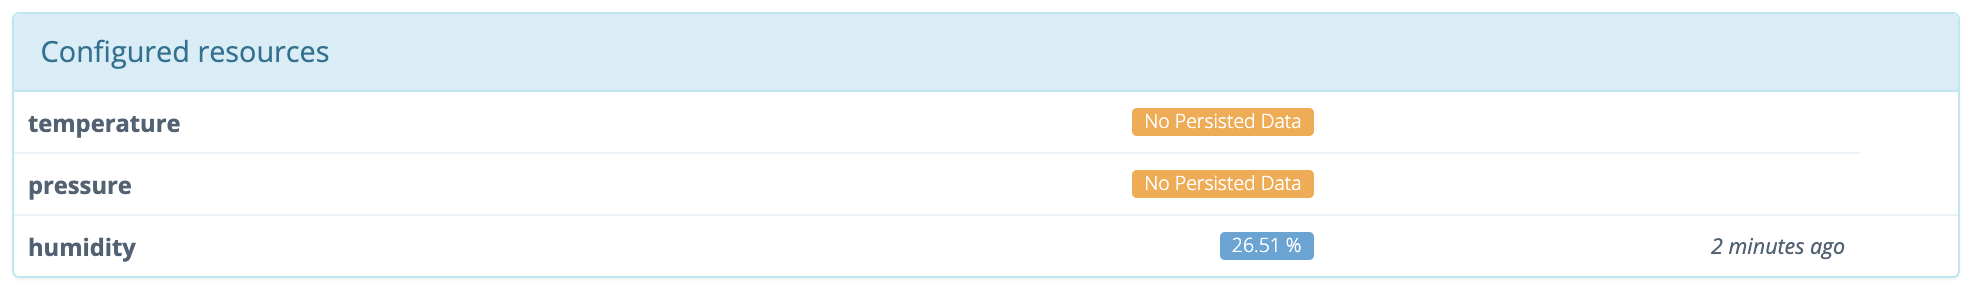
\includegraphics[width=1\columnwidth]{Pictures/bb_mesures.png}}
\lgf{\caption{État des ressources}}
\lge{\caption{Resource status}}
\label{fig-bb-mesure}
\end{figure}

\lgf{\subsection{Visualisation des ressources}}
\lge{\subsection{Resource visualization}}

\lgf{Maintenant que les ressources sont stockées dans les serveurs de Beebotte, il est possible de les visualiser graphiquement, en allant dans \textit{Dashboard} puis \textit{create Dashboard} et \textit {Add Widget} pour sélectionnez un widget comme \textit{Multi-line chart}.}
\lge{Now that the resources are stored in the Beebotte servers, it is possible to visualize them graphically, by going to \textit{Dashboard} and then \textit{create Dashboard} and \textit{Add Widget} to select a widget such as \textit{Multi-line chart}.}

\lgf{Puis, configurez le widget en définissant le canal et la ressource de ce canal comme le montre la figure~\vref{fig-widget}.}
\lge{Then, configure the widget by setting the channel and the resource for that channel as shown in figure~\vref{fig-widget}.}

\begin{figure}[tbp]
\centerline{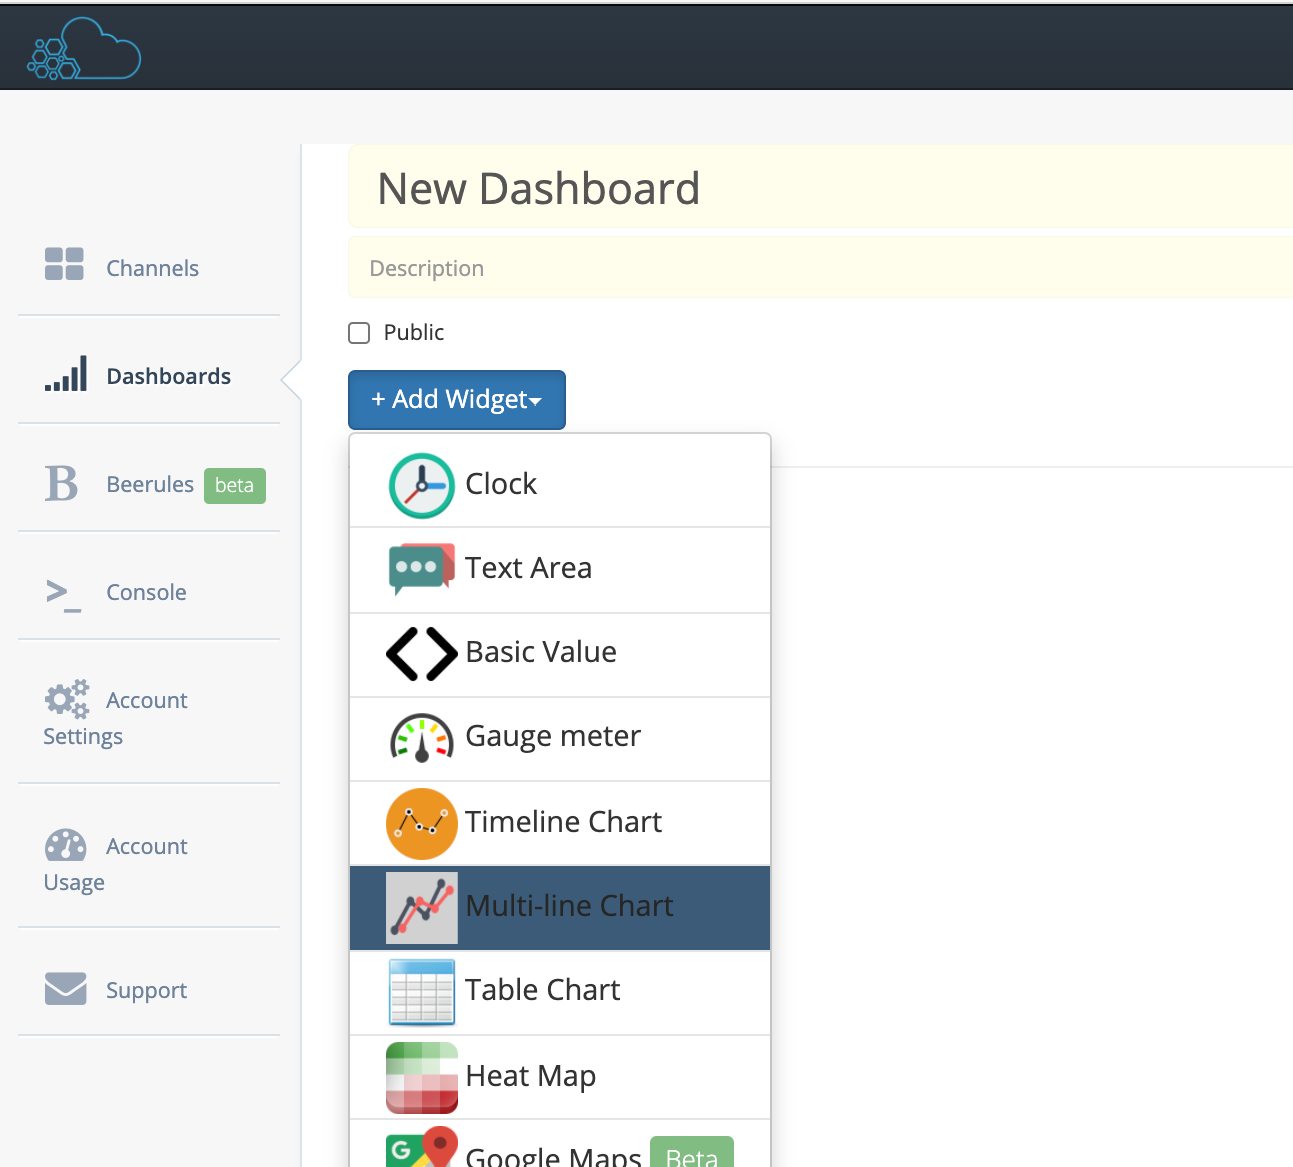
\includegraphics[width=0.5\columnwidth]{Pictures/bb_new_widget.png}}
       \vspace{1em}
\centerline{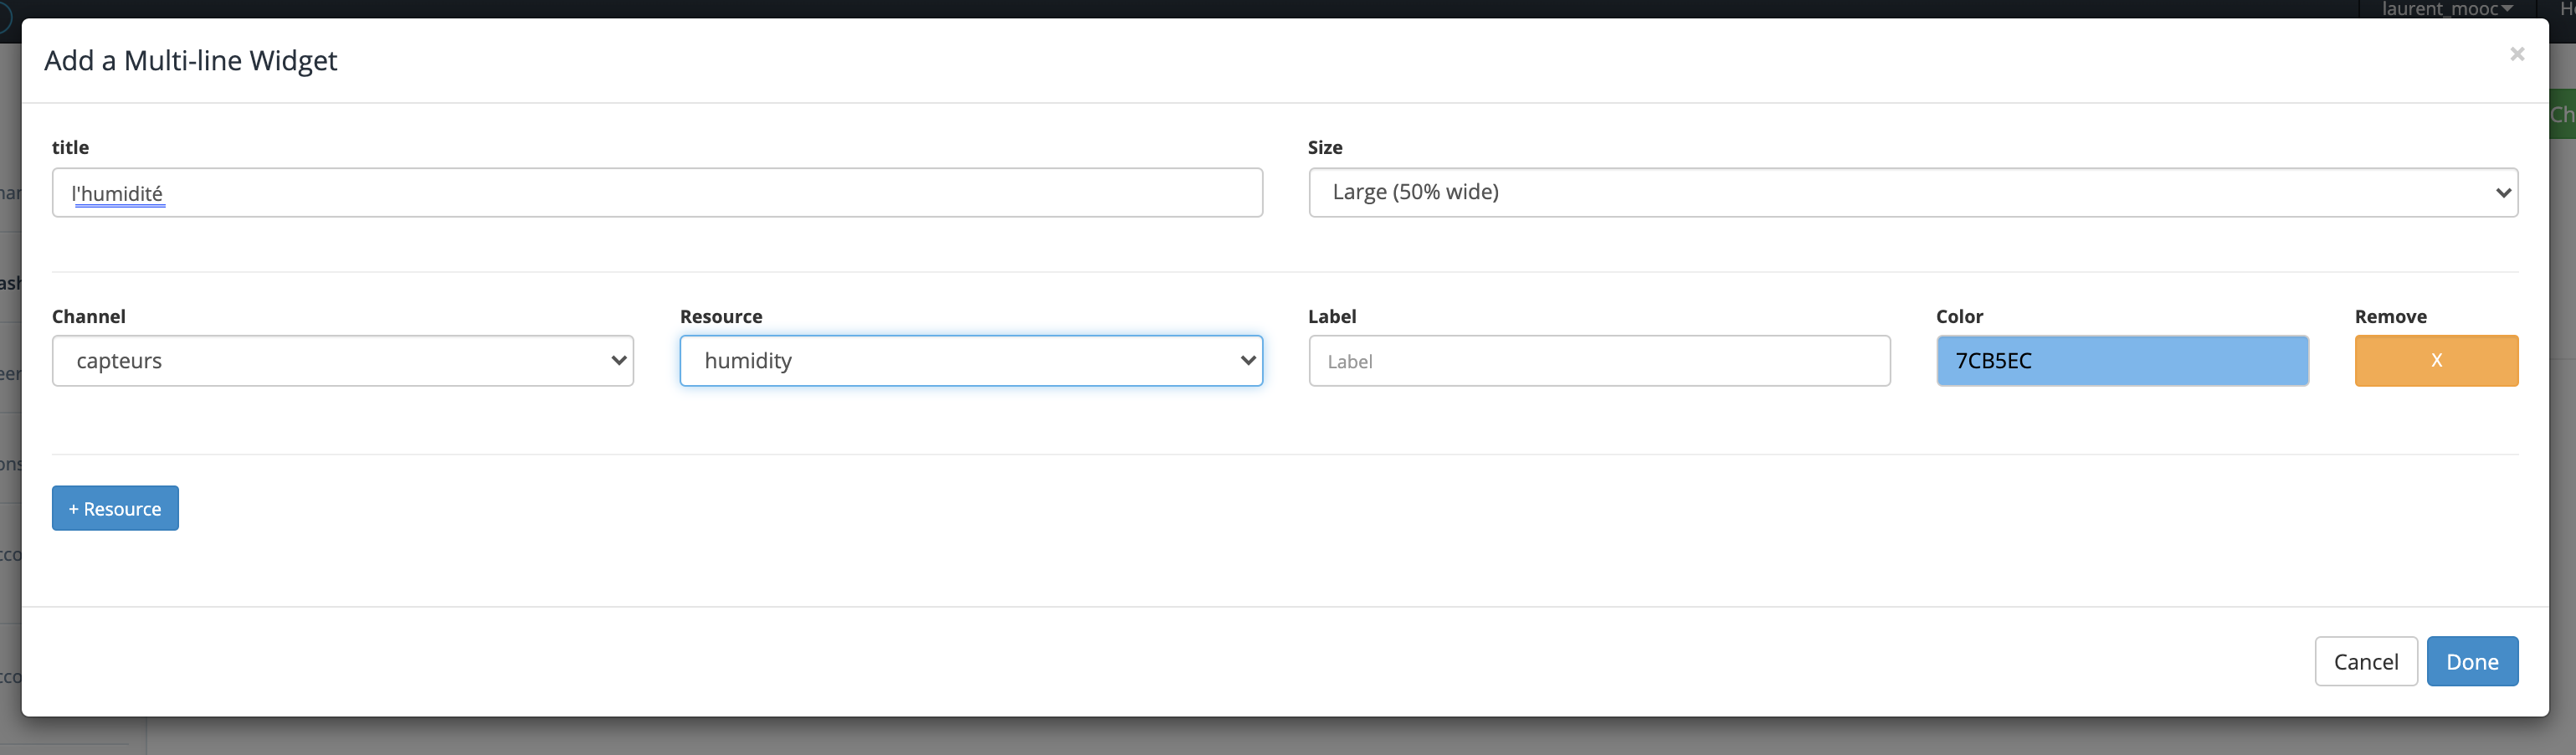
\includegraphics[width=0.5\columnwidth]{Pictures/bb_conf_widget.png}}
\lgf{\caption{Création d'un widget}}
\lge{\caption{Creating a widget}}
\label{fig-widget}
\end{figure}

\lgf{En retournant sur le dashboard, on peut voir l’évolution de l’humidité au cours du temps (cf. figure~\vref{fig-bb-humidity}). }
\lge{By going back to the dashboard, we can see the evolution of the humidity over time (see figure~\vref{fig-bb-humidity}). }

\begin{figure}[tbp]
\centerline{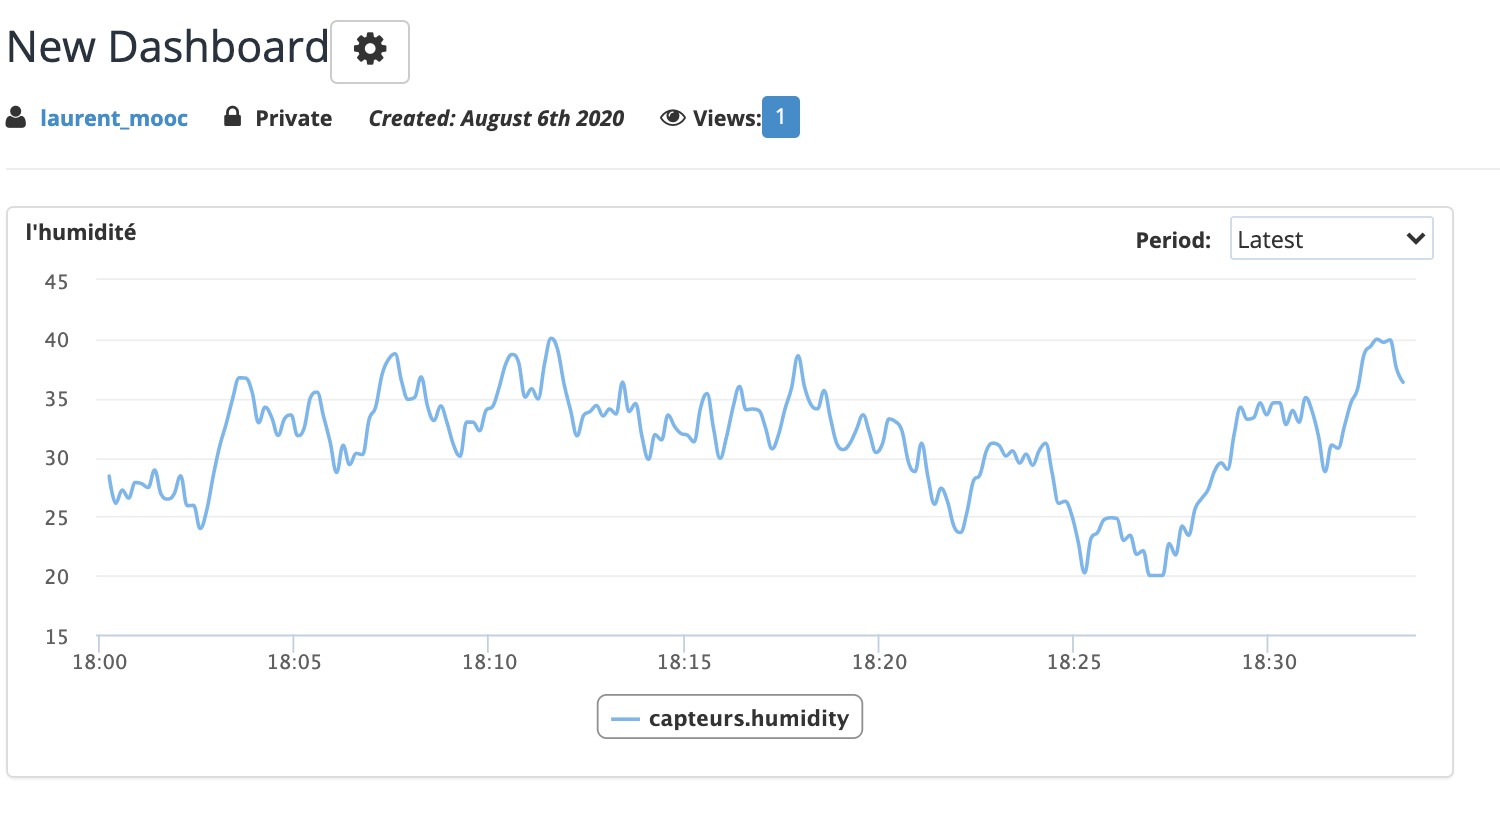
\includegraphics[width=1\columnwidth]{Pictures/bb_humidity.png}}
\lgf{\caption{Suivi de l'humidité}}
\lge{\caption{Humidity monitoring}}
\label{fig-bb-humidity}
\end{figure}

\lgf{\section{Interopérabilité}}
\lge{\section{Interoperability}}

\lgf{La chaîne de collecte de l'information que nous venons de construire allant du capteur à l'affichage, n'est pas complètement interopérable. Certes le capteur envoie des données au format CBOR qui peuvent être interprété par l'autre extrémité, mais le récepteur ne sait pas~:}
\lge{The chain of information collection that we have just built, from the sensor to the display, is not completely interoperable. Certainly the sensor sends data in CBOR format that can be interpreted by the other end, but the receiver does not know:}

\begin{itemize}
    \item 
        \lgf{qu'il s'agit d'une série temporelle codée avec des deltas~;}
        \lgf{that it is a coded time series with deltas;}
    \item  
        \lgf{que les données ont été multipliée par 100 pour pouvoir envoyer des nombres entiers, plus compacts sans perdre trop de précision~;}
        \lgf{that the data have been multiplied by 100 to be able to send whole numbers, more compact without losing too much precision;}
    \item  
        \lgf{que le pas de mesure est de 10 secondes~;}
        \lgf{that the measurement step is 10 seconds;}
    \item  
        \lgf{que les données concernent le taux d'humidité.}
        \lgf{that the data are related to the moisture content.}
\end{itemize}

\lgf{Ces informations ont été précisées dans le programme \pprog{display\_server.py}{plido-tp3}, de même la transformation de la structure de tableau de la série temporelle en un dictionnaire avec des mots clés spécifique à Beebotte on été gravé dans le programme. }
\lge{This information was specified in the program \pprog{display_server.py}{plido-tp3}, as well as the transformation of the table structure of the time series into a dictionary with keywords specific to Beebotte was engraved in the program. }

       \vspace{1em}

\lgf{Nous verrons par la suite comment améliorer cette interopérabilité.}
\lge{We will see later on how to improve this interoperability.}

\lgf{\section{et SenML ?}}
\lge{\section{and SenML?}}

\lgf{Dans la communication avec Beebotte,  le site structure l’envoi des mesures en définissant un dictionnaire JSON avec des mots clés particuliers. Pour utiliser un autre site, le format des échanges doit êter modifié même si les informations restent identiques.}
\lge{In the communication with Beebotte, the site structures the sending of measurements by defining a JSON dictionary with particular keywords. To use another site, the exchange format must be modified even if the information remains identical.}

       \vspace{1em}

\lgf{De plus, lors de la configuration des ressources sur le site de Beebotte, la nature de la mesure a du être précisée~; par exemple, s’il s’agit d’une température, d’un taux d’humidité... Il faut également parfois indiquer le type de la mesure (texte, entier, flottant...) voire les unités. }
\lge{In addition, when configuring the resources on the Beebotte site, the nature of the measurement had to be specified; for example, whether it is a temperature, a humidity level... It is also sometimes necessary to indicate the type of measurement (text, integer, float...) and even the units. }

       \vspace{1em}

\lgf{\ac{SenML} défini dans le \rfc{8428} propose une structuration des données fournie par le capteur. 
Pour réduire l’impact de la transmission, les noms des champs ont été choisis pour être le plus compact possible. 
Par exemple, la lettre \texttt{v}  va indiquer une valeur (à comparer avec la clé \texttt{data} utilisée lors de la communication avec Beebotte). 
Pour être encore plus compact, la représentation en CBOR utilisera des entiers courts au lieu de caractères.}
\lge{\ac{SenML} defined in the \rfc{8428} structures the data provided by the sensor. 
To reduce the impact of the transmission, the field names have been chosen to be as compact as possible. 
For example, the letter \texttt{v} will indicate a value (to be compared with the key \texttt{data} used during the communication with Beebotte). 
To be even more compact, the representation in CBOR will use short integers instead of characters.}

       \vspace{1em}

\lgf{Il est également possible de transporter l’unité de la mesure avec le mot clé \texttt{u} .}
\lge{It is also possible to transport the unit of measurement with the keyword \texttt{u} .}

\lgf{SenML ne définit pas que des unités  du système international, mais également des unités secondaires pour limiter la taille de la représentation. Il sera plus compact de transmettre~:}
\lge{SenML does not only define units of the international system, but also secondary units to limit the size of the representation. It will be more compact to transmit:}

\begin{termc}[backgroundcolor=\color{palerod}, basicstyle=\ttfamily\small, escapechar=\#]
{"u": "MHz", "v": 868}
\end{termc}

\noindent
\lgf{que}
\lge{than}

\begin{termc}[backgroundcolor=\color{palerod},  basicstyle=\ttfamily\small, escapechar=\#]
{"u": Hz", "v": 868000000}.
\end{termc}

\lgf{Le standard définit aussi des temps de base et des valeurs de base auxquelles les temps et les valeurs vont se référer ; ce qui permet également de réduire la taille des valeurs. Finalement, le ou les objets peuvent s’identifier dans les données transmises en définissant un nom de base (\texttt{bn} : \textit{base name}), le nom du capteur (\texttt{n} : \textit{name}) vient compléter le nom de base.}
\lge{The standard also defines base times and base values to which the times and values will refer; this also makes it possible to reduce the size of the values. Finally, the object(s) can be identified in the transmitted data by defining a base name (\texttt{bn} : \textit{base name}), the name of the sensor (\texttt{n} : \textit{name}) completes the base name.}

\lgf{\subsubsection{Émission}}
\lge{\subsubsection{Sending}}

\pythonlst{minimal\_senml\_client.py}

\lgf{Le programme \pprog{minimal\_senml\_client.py}{plido-tp3} illustre le fonctionnement de SenML. Il repose sur deux objets~:}
\lge{The program \pprog{minimal_senml\_client.py}{plido-tp3} illustrates how SenML works. It is based on two objects:}

\begin{itemize}
    \item
        \lgf{l'objet \pfunction{kpn\_senml}{SenmlPack} inclus les informations commune à l'objet, comme le nom de base (ici \texttt{device1} ligne 23) ou la base de temps, ligne 24.}
        \lge{the object \pfunction{kpn\_senml}{SenmlPack} includes information common to the object, such as the base name (here \texttt{device1} line 23) or the time base, line 24.}
    \item 
        \lgf{l'objet \pfunction{kpn\_senml}{SenmlRecord} contient une mesure où l'on peut préciser son nom, son unité et sa valeur (lignes 32, 38 et 44). Le temps est également précisé lignes 35, 41 et 47. Ces enregistrements sont ajoutés à l'objet \texttt{pack}.}
        \lge{the object \pfunction{kpn\_senml}{SenmlRecord} contains a measure where we can specify its name, its unit and its value (lines 32, 38 and 44). The time is also specified on lines 35, 41 and 47. These records are added to the \texttt{pack} object.}
\end{itemize}

\lgf{Le programme récupère les trois valeurs de température, humidité et pression (lignes 27 à 29) en les arrondissant à 2 chiffres après la virgule pour la température et l'humidité et converti la pression, d'hecto Pascal en Pascal puisque c'est l'unité définie par SenML. }
\lge{The program retrieves the three values of temperature, humidity and pressure (lines 27 to 29) by rounding them to 2 digits after the decimal point for temperature and humidity and converts the pressure from hecto Pascal to Pascal since this is the unit defined by SenML. }

\lgf{Les mesures se font toutes les 10 seconde (délais ligne 48) et quand le nombre de mesures défini ligne 13 est atteint, le codage SenML en CBOR est envoyé au serveur. }
\lge{Measurements are made every 10 seconds (delays line 48) and when the number of measurements defined on line 13 is reached, the SenML coding in CBOR is sent to the server. }

       \vspace{1em}

\begin{termc}[backgroundcolor=\color{palerod}, basicstyle=\ttfamily\small, escapechar=\#]
[{'bn': 'device1',
  'bt': 1650463643.0,
  'n': 'temperature',
  't': 0.0,
  'u': 'Cel',
  'v': 20.08},
 {'n': 'humidity', 't': 0.0, 'u': '%RH', 'v': 31.1},
 {'n': 'pressure', 't': 0.0, 'u': 'Pa', 'v': 99920}]
JSON length:  197 bytes
CBOR length:  126 bytes
\end{termc}

\lgf{Ce premier listing montre le premier enregistrement pour les trois grandeurs mesurées. Il s'agit d'un tableau de 3 éléments. Le premier contient les valeurs de bases (ici le nom et l'heure de référence) suivi de la grandeur à mesurer, de son unité et sa valeur. Le deuxième et le troisième éléments, mettent à jours le nom de la grandeur, son unité et sa valeur, les autres informations précédemment définies restent valables.}
\lge{This first listing shows the first record for the three measured quantities. It is a table of 3 elements. The first contains the basic values (here the name and the reference time) followed by the quantity to be measured, its unit and its value. The second and third elements update the name of the quantity, its unit and its value, the other information previously defined remains valid.}


\begin{termc}[backgroundcolor=\color{palerod},  basicstyle=\ttfamily\small, escapechar=@]
[@\textcolor{gray}{\{'bn': 'device1',}@
 @\textcolor{gray}{ 'bt': 1650463643.0,}@
 @\textcolor{gray}{ 'n': 'temperature',}@
 @\textcolor{gray}{ 't': 0.0,}@
 @\textcolor{gray}{ 'u': 'Cel',}@
 @\textcolor{gray}{ 'v': 20.08\},}@
 @\textcolor{gray}{\{'n': 'humidity', 't': 0.0, 'u': '\%RH', 'v': 31.1\},}@
 @\textcolor{gray}{\{'n': 'pressure', 't': 0.0, 'u': 'Pa', 'v': 99920},\}@
 {'n': 'temperature', 't': 10.0, 'u': 'Cel', 'v': 20.04},
 {'n': 'humidity', 't': 10.0, 'u': '%RH', 'v': 31.49},
 {'n': 'pressure', 't': 10.0, 'u': 'Pa', 'v': 99872}]
JSON length:  361 bytes
CBOR length:  232 bytes
 \end{termc}
 
 \lgf{Quand on ajoute 10 secondes plus tard de nouvelles mesures,  un temps relatif de 10 secondes est indiqué pour l'enregistrement des températures et il reste valable pour les enregistrements suivants.}
 \lge{When new measurements are added 10 seconds later, a relative time of 10 seconds is indicated for the temperature recording and it remains valid for the following recordings.}
 
 
 \Question{\lgf{Codage}\lge{Encoding}}
 {
 \lgf{A quoi correspond la clé \texttt{\{'u' : 'Cel'\}} que l'on retrouve dans la structure précédente ? }
 \lge{What does the key \texttt{\{'u' : 'Cel'\}} found in the previous structure correspond to? }
 }
 {
 \lgf{ Unité = degrés Celcius}
 \lge{ Unit = degrees Celcius}
 
 }
 
 \Question{\lgf{Accroissement}\lge{Growth}}
 {
 \lgf{Dans les deux représentations JSON et CBOR, de combien la taille est-elle accrue par l'ajout des mesures effectuées ? d'où viennent ces différences ?}
 \lge{In both JSON and CBOR representations, how much is the size increased by adding the measurements made? Where do these differences come from?}
 }
 {
 \lgf{Si l'on regarde le listing précédent, l'ajout des trois mesures fait augmenter la taille de 164 octets pour JSON et 106 pour CBOR. La différence vient de l'utilisation de nombre plus que de chaînes de caractères pour les clés. Ainsi 't' demande 3 caractères en JSON avec les guillemets, codé en CBOR, il faudrait 2 octets, un nombre inférieur à 23 se code sur un seul octet. Il y a egalement les virgules, espaces et fermeture de crochets qui ne sont pas présent en CBOR. Les nombres flottant comme \texttt{19.98} ont une représentation plus compacte en JSON (5 octets) qu'en CBOR où ils consomment 9 octets. Dans tous les cas l'accroissement est fortement dépendant du nom des éléments. Ici, il faut répéter à chaque fois \texttt{temperature}, \texttt{humidity} et \texttt{pressure}, soit 26 caractères.}
 \lge{If we look at the previous listing, adding the three measures increases the size by 164 bytes for JSON and 106 for CBOR. The difference comes from the use of numbers rather than strings for the keys. Thus 't' requires 3 characters in JSON with the quotes, encoded in CBOR, it would take 2 bytes, a number less than 23 is encoded on a single byte. There are also commas, spaces and closing brackets which are not present in CBOR. The floating numbers like \texttt{19.98} have a more compact representation in JSON (5 bytes) than in CBOR where they consume 9 bytes. In all cases the increase is strongly dependent on the name of the elements. Here, it is necessary to repeat each time \texttt{temperature}, \texttt{humidity} and \texttt{pressure}, that is 26 characters.}
 }
 
 \Question {\lgf{Une seule grandeur}\lge{A single value}}
 {
 \lgf{Si on ne s'intéressait qu'à une seule grandeur, par exemple l'humidité. A quoi ressemblerait la structure SenML en JSON ?}
 \lge{If we were only interested in one quantity, for example humidity. What would the SenML structure look like in JSON?}
 }
 {
 \lgf{Chaque nouvelle entrée ajoute 35 octets à la structure~: }
 \lge{Each new entry adds 35 bytes to the structure~: }
 
 \noindent
 [\{'bn': 'device1',  'bt': 1640110457.0, 'n': 'humidty', 'u': '\%RH', 'v': 28.46\},\\
 \{'t': 10.0, 'v': 26.86\},\\
 \{'t': 20.0, 'v': 26.96\},\\
 \{'t': 30.0, 'v': 27.01\}]\\
 }
 
 \lgf{\subsubsection{Réception}}
 \lge{\subsubsection{Receiving}}
 
 \lgf{Le traitement par le module SenML tel qu'il est mis en œuvre n'est pas complet, il ne gère pas correctement les timestamps. Mais, il n'est pas vraiment nécessaire pour traiter ces messages. En effet, comme on l'a vu précédemment, les valeurs SenML sont composés d'une base et d'une valeur. En concaténant les différents éléments du tableau, on garde les clés de base et on remplace les clés qui se répètent à chaque éléments. Cela permet d'avoir une mise en \oe{}uvre très simple du décodage, pour la série SenML qui nous est fournie.}
 \lge{The processing by the SenML module as implemented is not complete, it does not handle timestamps correctly. But, it is not really necessary to process these messages. Indeed, as we have seen previously, SenML values are composed of a base and a value. By concatenating the different elements of the array, we keep the base keys and we replace the keys which are repeated at each element. This allows to have a very simple implementation of the decoding, for the SenML series which is provided to us.}
 
 
 \pythonlst{minimal\_senml\_server.py}
 
 \lgf{Le programme \pprog{minimal\_senml\_server.py}{plido-tp3} va convertir le format SenML codé en CBOR dans le format attendu par Beebotte. 
 La version CBOR utilise des nombres plutôt que des tags.
 Le dictionnaire \texttt{naming\_map} defini lignes 10 à 12 permet la correspondance utilisé par la suite pour rendre le code plus lisible.}
 \lge{The program \pprog{minimal\_senml\_server.py}{plido-tp3} will convert the SenML format encoded in CBOR into the format expected by Beebotte. 
 The CBOR version uses numbers rather than tags.
 The dictionary \texttt{naming\_map} defined on lines 10 to 12 allows the correspondence used afterwards to make the code more readable.}
 
 \lgf{Les lignes 14 à 17 initialisent les communications venant du capteur et celles allant à Beebotte. }
 \lge{Lines 14 to 17 initialize the communications coming from the sensor and those going to Beebotte. }
 
\lgf{Les données reçues ligne 21 sont transformée en structure Python ligne 23. Cette correspondance est possible car Python autorise des clés numériques et celles-ci ne sont pas répétées plusieurs fois dans une map CBOR.}
\lge{The data received on line 21 is transformed into a Python structure on line 23. This correspondence is possible because Python allows numerical keys and these are not repeated several times in a CBOR map.}
 
\lgf{La boucle commençant ligne 28 permet d'explorer tous les éléments du tableau SenML, les nouvelles entrées sont fusionnées avec les anciennes (ligne 29)\footnote{Dans les version plus récentes de Python, il est possible d'utiliser l'opérateur \texttt{|}.}. }
\lge{The loop starting on line 28 allows you to explore all the elements of the SenML array, the new entries are merged with the old ones (line 29)\footnote{ In more recent versions of Python, it is possible to use the \texttt{|} operator.} }

\lgf{Les informations concernant le temps sont ensuite recherchées. 
D'abord le temps (ligne 32) et s'il un temps de base existe (ligne 33) il est ajouté. On procède de même pour la valeur (lignes 38 à 40). Pour le nom, il n'y a pas de concaténation car le nom de base sera utilisé comme canal Beebotte, il est récupéré à la fin ligne 46.}
\lge{The information about the time is then searched for. 
First the time (line 32) and if there is a basic time (line 33) it is added. The same procedure is followed for the value (lines 38 to 40). For the name, there is no concatenation because the basic name will be used as a Beebotte channel, it is recovered at the end of line 46.}

\lgf{A partir de ces informations, la structure attendue par Beebotte est construite ligne 43 en ajoutant le dictionnaire dans le tableau \texttt{bbt\_record}.}
\lge{From this information, the structure expected by Beebotte is constructed line 43 by adding the dictionary in the table \texttt{bbt\_record}.}

\lgf{Ligne 47, l'information est envoyée à Beebotte. Si les clés d'authentification, le nom du canal et des ressources sont correct, les information s'affiche sur le site, comme précédemment. }
\lge{Line 47, the information is sent to Beebotte. If the authentication keys, channel name and resources are correct, the information is displayed on the site, as before. }

\begin{termc}[backgroundcolor=\color{palerod},  basicstyle=\ttfamily\tiny, escapechar=@]
{0: 'temperature', 2: 19.94, 6: 0.0, 1: 'Cel', -2: 'device1', -3: 1650463732.0}
{0: 'humidity', 2: 27.7, 6: 0.0, 1: '%RH', -2: 'device1', -3: 1650463732.0}
{0: 'pressure', 2: 100109, 6: 0.0, 1: 'Pa', -2: 'device1', -3: 1650463732.0}
{0: 'temperature', 2: 19.88, 6: 10.0, 1: 'Cel', -2: 'device1', -3: 1650463732.0}
{0: 'humidity', 2: 24.82, 6: 10.0, 1: '%RH', -2: 'device1', -3: 1650463732.0}
{0: 'pressure', 2: 100056, 6: 10.0, 1: 'Pa', -2: 'device1', -3: 1650463732.0}
{0: 'temperature', 2: 19.93, 6: 20.0, 1: 'Cel', -2: 'device1', -3: 1650463732.0}
{0: 'humidity', 2: 23.74, 6: 20.0, 1: '%RH', -2: 'device1', -3: 1650463732.0}
{0: 'pressure', 2: 100123, 6: 20.0, 1: 'Pa', -2: 'device1', -3: 1650463732.0}
{0: 'temperature', 2: 19.92, 6: 30.0, 1: 'Cel', -2: 'device1', -3: 1650463732.0}
{0: 'humidity', 2: 25.82, 6: 30.0, 1: '%RH', -2: 'device1', -3: 1650463732.0}
{0: 'pressure', 2: 100220, 6: 30.0, 1: 'Pa', -2: 'device1', -3: 1650463732.0}
{0: 'temperature', 2: 19.9, 6: 40.0, 1: 'Cel', -2: 'device1', -3: 1650463732.0}
{0: 'humidity', 2: 24.47, 6: 40.0, 1: '%RH', -2: 'device1', -3: 1650463732.0}
{0: 'pressure', 2: 100173, 6: 40.0, 1: 'Pa', -2: 'device1', -3: 1650463732.0}
[{'data': 19.94, 'resource': 'temperature', 'ts': 1650463732000.0},
 {'data': 27.7, 'resource': 'humidity', 'ts': 1650463732000.0},
 {'data': 100109, 'resource': 'pressure', 'ts': 1650463732000.0},
 {'data': 19.88, 'resource': 'temperature', 'ts': 1650463742000.0},
 {'data': 24.82, 'resource': 'humidity', 'ts': 1650463742000.0},
 {'data': 100056, 'resource': 'pressure', 'ts': 1650463742000.0},
 {'data': 19.93, 'resource': 'temperature', 'ts': 1650463752000.0},
 {'data': 23.74, 'resource': 'humidity', 'ts': 1650463752000.0},
 {'data': 100123, 'resource': 'pressure', 'ts': 1650463752000.0},
 {'data': 19.92, 'resource': 'temperature', 'ts': 1650463762000.0},
 {'data': 25.82, 'resource': 'humidity', 'ts': 1650463762000.0},
 {'data': 100220, 'resource': 'pressure', 'ts': 1650463762000.0},
 {'data': 19.9, 'resource': 'temperature', 'ts': 1650463772000.0},
 {'data': 24.47, 'resource': 'humidity', 'ts': 1650463772000.0},
 {'data': 100173, 'resource': 'pressure', 'ts': 1650463772000.0}]

 \end{termc}
 
 \lgf{Le listing précédent montre cette transformation.
 Les premières lignes correspondent aux enregistrements fusionnées et le tableau final, ce qui a été envoyé à Beebotte.}
 \lge{The previous listing shows this transformation.
 The first rows are the merged records and the final table is what was sent to Beebotte.}
 
 
 \Question{base value}
 {
 \lgf{Pourrait-on utiliser le champ SenML \textit{base value} pour diminuer la taille des données de pression atmosphérique~?}
 \lge{Could we use the SenML field \textit{base value} to decrease the size of the air pressure data~?}
 }
 {
\lgf{Cela serait possible, si cette ressource était envoyée seule.}
\lge{This would be possible, if this resource was sent alone.}
 }
\cleardoublepage
\lgf{\chapter{Découvrons le LoPy}}
\lge{\chapter{Discover the LoPy}}

\lgf{\textit{Les programmes relatifs à cette section se trouvent dans le répertoire \texttt{plido-tp3} pour le serveur et \texttt{pycom} pour le LoPy.}}
\lge{\textit{The programs related to this section are located in the \texttt{plido-tp3} directory for the server and \texttt{pycom} for the LoPy.}}


\section{Introduction}

\lgf{Grâce aux émulateurs de capteurs décrits au chapitre précédent, vous avez pu appliquer les concepts essentiels de l'IoT sur votre ordinateur.}
\lge{Using the sensor emulators described in the previous chapter, you have been able to apply the essential IoT concepts to your computer.}

\lgf{Cependant, si vous le pouvez, nous vous invitons à le faire sur de vrais objets connectés en utilisant des \Index{LoPy4} (plateforme de prototypage IoT) de la société \Index{Pycom} et des capteurs de température, humidité et pression \Index{BME280} (cf. figure~\vref{fig-lopy-bme280}).}
\lge{However, if you can, we invite you to do it on real connected objects using \Index{LoPy4} (IoT prototyping platform) from the company \Index{Pycom} and temperature, humidity and pressure sensors \Index{BME280} (see figure~\vref{fig-lopy-bme280}).}


\begin{figure}[tbp]
\centerline{\includegraphics[width=.5\columnwidth]{Pictures/LoPy.jpg}  \includegraphics[width=.3\columnwidth]{Pictures/BME280.jpeg}}
\lgf{\caption{LoPY4 et capteur BME280}}
\lge{\caption{LoPY4 and BME280 sensor}}
\label{fig-lopy-bme280}
\end{figure}

\lgf{Un LoPY4 se programme en Python (ou plutôt \Index{micro-python} qui est la version du langage pour systèmes embarqués) pour traiter les données. Dans un premier temps, nous allons utiliser le Wi-Fi pour communiquer avec votre ordinateur mais, par la suite, nous mettrons en place une communication via \Index{LoRaWAN} ou \Index{Sigfox} qui peut vous demander plus de configuration mais vous permettra de mieux comprendre ces protocoles.}
\lge{A LoPY4 is programmed in Python (or rather \Index{micro-python} which is the version of the language for embedded systems) to process data. At first, we will use Wi-Fi to communicate with your computer but, later, we will set up a communication via \Index{LoRaWAN} or \Index{Sigfox} which may require more configuration but will allow you to better understand these protocols.}


     \vspace{1em}


\lgf{Même si vous n’avez pas de LoPy4, vous pouvez parcourir cette section pour voir les contraintes supplémentaires liées aux objets connectés.}
\lge{Even if you don't have LoPy4, you can browse this section to see additional constraints related to connected objects.}


\lgf{\section{Installation d'Atom}}
\lge{\section{Installing Atom}}


\lgf{\Index{Atom} est un éditeur de texte performant, spécifiquement conçu pour le codage en différents langages. 
Atom va nous aider à programmer en Python et va également gérer la communication avec notre LoPy via le port \Index{USB} (grâce au plugin \Index{pymakr}). 
Atom fonctionne à peu près de la même manière sur \Index{Mac OS}, \Index{Windows} et \Index{Linux}, mais en s’adaptant aux particularités du système d’exploitation (place dans les menus, nom des liens séries...). 
Donc, il se peut que vous ayez quelques différences entre ce que vous avez dans cet ouvrage et l’écran de votre ordinateur. 
Les menus et sites Web indiqués peuvent également changer au cours du temps même si nous nous efforçons de faire des mises à jour régulières du cours.}
\lge{\Index{Atom} is a powerful text editor, specifically designed for coding in different languages. 
Atom will help us to program in Python and will also manage the communication with our LoPy via the \Index{USB} (thanks to the plugin \Index{pymakr}). 
Atom works in much the same way on \Index{Mac OS}, \Index{Windows} and \Index{Linux}, but it adapts to the particularities of the operating system (place in the menus, name of the serial links...). 
So, you may have some differences between what you have in this book and the screen of your computer. 
The menus and websites shown may also change over time, although we try to update the course regularly.}


     \vspace{1em}

\lgf{Pour commencer à programmer avec votre LoPy, vous devez installer sur votre ordinateur le logiciel Atom (voir sur \url{http://atom.io}). 
Vous pouvez télécharger le package correspondant à votre système d'exploitation (cf. figure suivante).}
\lge{To start programming with your LoPy, you must install on your computer the Atom software (see \url{http://atom.io}). 
You can download the package corresponding to your operating system (see next figure).}


\begin{figure}[tbp]
\centerline{\includegraphics[width=1\columnwidth]{Pictures/atom_dl.png}}
\lgf{\caption{Page d'accueil d'Atom}}
\lge{\caption{Atom homepage}}
\label{fig-page-atom}
\end{figure}


\begin{itemize}
\item 
    \lgf{Pour Mac et Windows, cliquez sur l’icône "télécharger" pour l’installer\footnote{il y a des risques d'incompatibilité des dernières versions d'Atom avec le package de gestion du LoPy (pymakr). Nous vous recommandons d'utiliser une version plus ancienne, comme la 1.43 disponible dans les archives d'Atom Release \url{https://github.com/atom/atom/releases/tag/v1.43.0}(\texttt{AtomSetup-x64.exe} pour Windows ou \texttt{atom-mac.zip} pour Mac OS).}.}
    \lge{For Mac and Windows, click on the "download" icon to install it. There is a risk of incompatibility between the latest versions of Atom and the LoPy management package (pymakr). We recommend you to use an older version, like the 1.43 available in the Atom Release archives (\url{https://github.com/atom/atom/releases/tag/v1.43.0}(\texttt{AtomSetup-x64.exe} for Windows or \texttt{atom-mac.zip} for Mac OS).}    
\item 
    \lgf{Pour Linux, téléchargez le\texttt{.deb} et tapez \texttt{sudo dpkg -i atom-amd64.deb}\footnote{Il est possible qu'un message vous dise que git n'est pas installé. Dans ce cas, tapez \texttt{sudo apt-get install git} et suivez les instructions).}.
    Lancez Atom en cliquant sur l’icône ou, sous Linux, en tapant atom dans un terminal.}
    \lge{For Linux, download letexttt{.deb} and type \texttt{sudo dpkg -i atom-amd64.deb}\footnote{It is possible that a message tells you that git is not installed. In this case, type \texttt{sudo apt-get install git} and follow the instructions}.
    Launch Atom by clicking on the icon or, under Linux, by typing atom in a terminal.}
\end{itemize}

     \vspace{1em}

\lgf{Lancez Atom en cliquant sur l’icône ou, sous Linux, en tapant atom dans un terminal. L’écran d’accueil apparaît.}
\lge{Launch Atom by clicking on the icon or, under Linux, by typing atom in a terminal. The welcome screen appears.}


\lgf{\subsection{Communiquez avec votre Pycom}}
\lge{\subsection{Communicate with your Pycom}}


\lgf{Pour communiquer avec le Pycom à travers Atom, vous devez installer le package \texttt{\Index{pymakr}}.}
\lge{To communicate with the Pycom through Atom, you must install the \texttt{\Index{pymakr}} package.}

\lgf{Cliquez sur \textit{Install a Package} puis \textit{Open Installer}. Une autre fenêtre s’ouvre (cf. figure~\vref{fig-page-pakage}. Tapez \texttt{pymakr} dans le menu. Un package apparaît portant ce nom. Cliquez sur \textit{Install}. L’installation peut prendre plusieurs minutes. Vous avez le temps de prendre un café.}
\lge{Click on \textit{Install a Package} then \textit{Open Installer}. Another window will open (see figure~\vref{fig-page-pakage}. Type \texttt{pymakr} in the menu. A package with this name appears. Click on \textit{Install}. The installation may take several minutes. You have time to have a coffee.}


\begin{figure}[tbp]
\centerline{\includegraphics[width=1\columnwidth]{Pictures/atom_pymakr.png}}
\lgf{\caption{Installation de Paquetages}}
\lge{\caption{Package Installation}}
\label{fig-page-pakage}
\end{figure}

     \vspace{1em}

\lgf{Une fois le café bu et l’installation terminée, une nouvelle fenêtre (terminal) s’ouvre en bas d’Atom.}
\lge{Once the coffee is drunk and the installation is finished, a new window (terminal) opens at the bottom of Atom.}

     \vspace{1em}

\lgf{Ce terminal (cf.figure~\vref{fig-page-pymakr}) vous permettra de dialoguer avec le LoPy.
Branchez le LoPy à votre ordinateur.
Vous devriez voir l’invite\texttt{ >{}>{}>{}} caractéristique d’un interpréteur Python\footnote{Sous Linux, vous devez être membre du groupe dialout pour pouvoir gérer la communication sur le port USB. 
Si vous ne voyez par l’invite, tapez \texttt{sudo adduser \textit{login} dialout} en remplaçant login par le nom de votre compte Linux. Reconnectez-vous sous votre compte.}.}
\lge{This terminal (cf.figure~\vref{fig-page-pymakr}) will allow you to dialogue with the LoPy.
Connect the LoPy to your computer.
You should see the typical Python interpreter prompt \texttt{>{}>{}>{}}\footnote{Under Linux, you must be a member of the dialout group to be able to manage the communication on the USB port. 
If you do not see the prompt, type \texttt{sudo adduser \textit{login} dialout} replacing login with the name of your Linux account. Reconnect under your account}.}


     \vspace{1em}

\begin{figure}[tbp]
\centerline{\includegraphics[width=1\columnwidth]{Pictures/atom_pymakr1.png}}
\lgf{\caption{Fenêtre Pymakr}}
\lge{\caption{Pymakr window}}
\label{fig-page-pymakr}
\end{figure}

\lgf{Toutes les commandes que vous allez taper dans cette fenêtre vont s’exécuter sur votre LoPy. Par exemple, si vous tapez\footnote{Les fenêtres sur fond gris montrent le code micropython et leur résultat.}~:}
\lge{All the commands you type in this window will run on your LoPy. For example, if you type \footnote{The windows with gray background show the micropython code and their result.}:}

\begin{termc}[backgroundcolor=\color{gray!10}, basicstyle=\ttfamily\small, escapechar=@]
Connecting to /dev/ttyUSB0...
>>> @\textbf{1+1}@
2
>>>
\end{termc}

\noindent
\lgf{l’addition se fait sur le LoPy.}
\lge{the addition is done on the LoPy.}


     \vspace{1em}

\lgf{Sur le coté gauche de la fenêtre pymakr, plusieurs icônes sont présentes~:}
\lge{On the left side of the pymakr window, several icons are present:}

\begin{itemize}
    \item 
        \lgf{l'interrupteur permet d'activer ou de désactiver le connexion avec le LoPy~;}
        \lge{the switch allows to activate or deactivate the connection with the LoPy;}
    \item  
        \lgf{le triangle permet d'exécuter le programme affiché dans la fenêtre d'Atom sur le LoPy~;}
        \lge{the triangle allows you to execute the program displayed in the Atom window on the LoPy;}
    \item  
        \lgf{la flèche vers le haut, permet de recopier le répertoire actif dans la mémoire du LoPy. Cela sera utile pour installer de nouveaux modules sur le LoPy~;}
        \lge{the up arrow, allows you to copy the active directory into the LoPy memory. This will be useful to install new modules on the LoPy;}
    \item  
        \lgf{inversement le flèche vers le bas, permet de recopier la mémoire du LoPy sur l'ordinateur~;}
        \lge{Conversely, the down arrow allows you to copy the memory of the LoPy to the computer;}
    \item  
        \lgf{le processeur permet d'avoir des informations sur le loPy.}
        \lge{the processor allows to have information about the loPy.}
\end{itemize}

     \vspace{1em}

\lgf{Sur la partie droite, l'onglet vertical \textit{Setting} permet de modifier les paramètres de connexion avec le LoPy.}
\lge{On the right side, the vertical tab \textit{Setting} allows to modify the connection parameters with the LoPy.}


\lgf{\subsection{Installez votre environnement de travail} }
\lge{\subsection{Set up your work environment} }

\lgf{Pour programmer le LoPy, il faut récupérer les modules micropython. Le dépôt ca être téléchargé dans le répertoire de votre choix~:}
\lge{To program the LoPy, you have to get the micropython modules. The repository can be downloaded in the directory of your choice:}


\begin{termc}[backgroundcolor=\color{gray!10},  basicstyle=\ttfamily\small, escapechar=@]
> git clone https://github.com/ltn22/PLIDObis.git
\end{termc}

\lgf{Dans le menu \textit{Files>Open Folder} d’Atom, sélectionnez le répertoire \texttt{pycom} du dépot téléchargé, et validez. Sur la partie gauche de l’écran, l’ensemble des fichiers composant ce répertoire apparaissent. Il y en a beaucoup, car ils vont nous servir par la suite.}
\lge{In Atom's \textit{Files>Open Folder} menu, select the \texttt{pycom} directory of the downloaded repository, and validate. On the left side of the screen, all the files composing this directory appear. There are a lot of them, because they will be used later.}


     \vspace{1em}

\lgf{En cliquant dans la fenêtre \textit{\Index{pymakr}} sur le bouton \textit{Upload project to device}, les fichiers de ce répertoire vont être copiés dans la mémoire du LoPy. 
Par la suite, si un module est modifié, il devra être resynchronisé dans la mémoire du LoPy.}
\lge{By clicking in the window \textit{Index{pymakr}} on the button \textit{Upload project to device}, the files of this directory will be copied in the memory of LoPy. 
Afterwards, if a module is modified, it will have to be resynchronized in the memory of LoPy.}

\lgf{\section{Connexion au réseau Wi-Fi}}
\lge{\section{Connection to the Wi-Fi network}}


\begin{wrapfigure}{r}{3cm}
\Youtube{https://youtu.be/PmvSU8AWO68}
\end{wrapfigure}


\lgf{Pour rattacher de LoPY à un réseau \Index{Wi-Fi}, il doit dans un premier temps être configuré via la liaison USB de l'ordinateur pour lui donner les paramètres nécessaires à la connexion. }
\lge{To attach LoPY to a \Index{Wi-Fi} network, it must first be configured via the USB link of the computer to give it the necessary parameters for the connection. }

\lgf{Le fichier \texttt{\Index{boot.py}} a été copié lors du téléversement des fichiers dans la mémoire du LoPy. Au démarrage du LoPy, ce programme va chercher à se connecte à un réseau Wi-Fi. Comme le nom du réseau et la clé sécrète n'ont pas été founie, il n’y arrive pas. Le LoPy se transforme  en point d’accès. Au démarrage, le LoPy a dû afficher le message suivant, indiquant que le LoPy devient point d'accès Wi-Fi et va déployer son propre réseau sur lequel votre ordinateur peut se connecter. Le nom de ce réseau de les la forme \texttt{PLIDO\_XXXX} où \texttt{XXXX} est une séquence hexadécimal propre à l'équipement. La clé est \texttt{www.pycom.io}. Le LoPy à l'adresse \texttt{192.168.4.1} sur ce réseau.  }
\lge{The file \texttt{Index{boot.py}} has been copied when uploading the files in the LoPy memory. When LoPy starts, this program will try to connect to a Wi-Fi network. As the network name and the secret key have not been provided, it does not succeed. The LoPy turns into an access point. At startup, the LoPy should have displayed the following message, indicating that the LoPy becomes a Wi-Fi access point and will deploy its own network on which your computer can connect. The name of this network has the form \texttt{PLIDO\_XXXX} where \texttt{XXXX} is a hexadecimal sequence specific to the equipment. The key is \texttt{www.pycom.io}. The LoPy at address \texttt{192.168.4.1} on this network.  }


\begin{termc}[backgroundcolor=\color{gray!10},  basicstyle=\ttfamily\small, escapechar=@]
Failed to connect to any known network, going into AP mode
To connect look for 'PLIDO_5bac' access point, key = 'www.pycom.io'
\end{termc}

\lgf{Mais ce n'est pas très intéressant car votre ordinateur va perdre sa connexion à l'internet. Pas très pratique pour suivre le MOOC. Avant d'afficher ce message, le LopY a montré la liste des réseaux Wi-Fi qu'il a détecté. Vous pouvez à l'inverse le connecter à un de ces réseau en renseignant le fichier \texttt{wifi\_conf.py} qui se trouve dans le répertoire \texttt{pycom}.}
\lge{But this is not very interesting because your computer will lose its connection to the internet. Not very practical to follow the MOOC. Before displaying this message, the LopY showed the list of Wi-Fi networks it detected. You can connect it to one of these networks by filling in the file \texttt{wifi\_conf.py} which is in the directory \texttt{pycom}.}

\pycomlst{wifi\_conf.py}

\lgf{\texttt{MON\_SSID} doit être remplacé par le nom du réseau Wi-Fi ou \ac{SSID} et \texttt{MON\_MOT\_DE\_PASSE} par la clé qui y est associée. Notez que plusieurs réseaux Wi-Fi peuvent être ajouté, puisque \texttt{MON\_SSID} est vu comme une clé de l'objet JSON. L'édition de fichier s'est faite sur l'ordinateur, il doit être recopié dans la mémoire du LoPy en cliquant sur la flèche vers le haut.}
\lge{\texttt{MON\_SSID} must be replaced by the name of the Wi-Fi network or \ac{SSID} and \texttt{MON\_MOT\_DE\_PASSE} by the key associated with it. Note that several Wi-Fi networks can be added, since \texttt{MON\_SSID} is seen as a key of the JSON object. The file edition was done on the computer, it must be copied in the memory of the LoPy by clicking on the up arrow.}

\lgf{Le Pycom redémarre et doit maintenant afficher un message du genre :}
\lge{The Pycom restarts and should now display a message like:}


\begin{termc}[backgroundcolor=\color{gray!10}, basicstyle=\ttfamily\small, escapechar=@]
net to use ['MONWIFI']
Connected to MONWIFI with IP address: @\ul{192.168.1.76}@
Pycom MicroPython 1.20.2.r1 [v1.11-a5aa0b8] on 2020-09-09; LoPy4 with ESP32
Type "help()" for more information.
>>> 
\end{termc}

\lgf{Il est possible de pinguer ou de se connecter avec \Index{FTP} ou \Index{telnet} en utilisant cette adresse IP.}
\lge{It is possible to ping or connect with \Index{FTP} or \Index{telnet} using this IP address.}

\begin{termc}[backgroundcolor=\color{palerod},  basicstyle=\ttfamily\small, escapechar=@]
# @\textbf{telnet \ul{192.168.1.76}}@
Trying 192.168.1.86...
Connected to 192.168.1.86.
Escape character is '^]'.
MicroPython v1.8.6-760-g90b72952 on 2017-09-01; LoPy with ESP32
Login as: micro
Password: python
Login succeeded!
Type "help()" for more information.
>>>
\end{termc}

\lgf{Ça peut être utile pour suivre le comportement de votre objet sans lancer atom si l'objet n'est plus connecté via la liaison USB à l'ordinateur. }
\lge{It can be useful to follow the behavior of your object without launching atom if the object is not connected via the USB link to the computer. }

\lgf{Atom peut également être configuré pour utiliser cette adresse IP. La configuration se fait dans le menu \textit{setting}, et en entrant l'adresse ip du LoPy et en désactivant \textit{auto connect}. Au prochain lancement d'Atom, il sera possible joindre le LoPy en Wi-Fi.}
\lge{Atom can also be configured to use this IP address. The configuration is done in the menu \textit{setting}, and by entering the ip address of the LoPy and disabling \textit{auto connect}. The next time Atom is launched, it will be possible to join the LoPy in Wi-Fi.}



\lgf{\section{Mise en place d'un client}}
\lge{\section{Setting up a client}}


\begin{wrapfigure}{r}{3cm}
\Youtube{https://youtu.be/Mi3e4c2E59o}
\end{wrapfigure}


\lgf{Un programme relativement simple permet de vérifier la communication entre le LoPy et le serveur. La commande \Index{ifconfig}\footnote{Sous Linux, il faut ajouter le paquetage \Index{net-tools} \texttt{sudo apt install net-tools}.} donne l'adresse IP du serveur. L'adresse doit être différente de celle que l'on avait obtenu sur le LoPy. }
\lge{A relatively simple program allows to check the communication between the LoPy and the server. The command \Index{ifconfig}\footnote{Under Linux, it is necessary to add the package \Index{net-tools} \texttt{sudo apt install net-tools}.} gives the server IP address. The address must be different from the one we had obtained on the LoPy. }

\lgf{Si le serveur tourne dans un environnement local, l'adresse devrait commencer par \texttt{192.168} ou \texttt{10}. Si le LoPy et l'ordinateur sont connectés au même réseau Wi-Fi, les premiers chiffres doivent être identiques. }
\lge{If the server is running in a local environment, the address should start with \texttt{192.168} or \texttt{10}. If the LoPy and the computer are connected to the same Wi-Fi network, the first digits must be identical. }

\lgf{Si le serveur tourne sur un serveur à l'extérieur (i.e. le \textit{cloud}), l'adresse est quelconque.}
\lge{If the server is running on an external server (i.e. the \textit{cloud}), the address is random.}

     \vspace{1em}

\lgf{La commande suivante est tapée depuis le terminal de l'ordinateur, on remarque les deux interfaces disponibles l'une pour le réseau Ethernet ou Wi-Fi et l'une pour le \textit{\Index{loopback}}, les noms des interfaces peuvent changer d'une configuration à une autre~:}
\lge{The following command is typed from the terminal of the computer, we notice the two available interfaces one for the Ethernet or Wi-Fi network and one for the \textit{\Index{loopback}}, the names of the interfaces can change from one configuration to another:}

\begin{termc}[backgroundcolor=\color{palerod},  basicstyle=\ttfamily\small, escapechar=@]
> @\textbf{ifconfig}@
eth1      Link encap:Ethernet  HWaddr 10:65:30:b0:54:bf
          inet addr:@\ul{192.168.1.237}@  Bcast:192.168.1.255  Mask:255.255.255.0
          inet6 addr: fe80::d8ac:86e7:8bdb:e333/64 Scope:Unknown
          UP BROADCAST RUNNING MULTICAST  MTU:1500  Metric:1
          RX packets:0 errors:0 dropped:0 overruns:0 frame:0
          TX packets:0 errors:0 dropped:0 overruns:0 carrier:0
          collisions:0
          RX bytes:0 (0.0 B)  TX bytes:0 (0.0 B)

lo        Link encap:Local Loopback
          inet addr:127.0.0.1  Mask:255.0.0.0
          inet6 addr: ::1/128 Scope:Unknown
          UP LOOPBACK RUNNING  MTU:1500  Metric:1
          RX packets:0 errors:0 dropped:0 overruns:0 frame:0
          TX packets:0 errors:0 dropped:0 overruns:0 carrier:0
          collisions:0
          RX bytes:0 (0.0 B)  TX bytes:0 (0.0 B)
\end{termc}

\lgf{Le programme \pprog{minimal\_server.py}{plido-tp3} présenté au chapitre~\vref{chap-mini-serv} n'a pas été modifié et attend des données sur le port 33033.}
\lge{The program \pprog{minimal\_server.py}{plido-tp3} presented in chapter~\vref{chap-mini-serv} has not been modified and waits for data on port 33033.}


     \vspace{1em}

\pycomlst{sending\_client.py}

\lgf{Le programme \lprog{sending\_client.py}{pycom} doit être modifié (ligne 4) pour prendre en compte l'adresse IP du serveur obtenue avec la commande \texttt{ifconfig}. Si à chaque exécution sur le LoPy de ce programme, le serveur reçoit la valeur, la communication est établie entre les deux équipements.}
\lge{The program \lprog{sending\_client.py}{pycom} must be modified (line 4) to take into account the IP address of the server obtained with the command \texttt{ifconfig}. If at each execution on the LoPy of this program, the server receives the value, the communication is established between the two devices.}


\begin{termc}[backgroundcolor=\color{palerod}, basicstyle=\ttfamily\small, escapechar=@]
> @\textbf{python3 minimal\_server.py}@
b'message' => b'6d657373616765'
b'message' => b'6d657373616765'
\end{termc}


\section{BME 280}

\begin{wrapfigure}{r}{3cm}
\Youtube{https://youtu.be/I3zc3-qoq2s}
\end{wrapfigure}

\lgf{Au lieu de générer de fausses données, nous allons dans cette section utiliser un vrai capteur de température humidité pression : le BME 280 de chez Bosch. }
\lge{Instead of generating false data, we will use in this section a real temperature humidity pressure sensor: the BME 280 from Bosch. }


\lgf{\subsection{Le bus I2C}}
\lge{\subsection{I2C bus}}


\lgf{Le bus I2C est  normalisé par le fabricant de composants électroniques  \Index{NXP}\footnote{\url{https://www.nxp.com/docs/en/user-guide/UM10204.pdf}} ce qui permet une meilleure interopérabilité entre les composants.}
\lge{The I2C bus is standardized by the electronic components manufacturer \Index{NXP}\footnote{url{https://www.nxp.com/docs/en/user-guide/UM10204.pdf}} which allows a better interoperability between the components.}


 \begin{figure}[!ht] 
\centering 


	\begin{tikzpicture}
	
	\draw [thick, red] (0, 7.5) node [left] {3.3V} coordinate (l1) -- +(12, 0); 
	\draw [thick, black] (0, 7) node [left] {GND} coordinate (l2) -- +(12, 0); 
	
	\draw [thick, yellow!80!black] (0, 3) node [left] {SCL} coordinate (l3) -- +(12, 0); 
	\draw [thick, green] (0, 2.5) node [left] {SDA} coordinate (l4) -- +(12, 0); 
	
	\foreach \i/\n in {1/Primary, 2/Secondary 1, 3/Secondary 2, 4/Secondary 3} {
		\draw (2.5*\i, 5) node (n\i) [rectangle, top color=blue!40, bottom color=blue!20, draw, minimum size= 2cm]{};
		
		\draw (n\i) node {\n};
		
		\filldraw [red] (n\i.120) -- (n\i.120 |-l1) circle  (2pt);
		\filldraw [black] (n\i.60) -- (n\i.60 |-l2) circle  (2pt);
		\filldraw [yellow!80!black] (n\i.-120) -- (n\i.-120 |-l3) circle  (2pt);
		\filldraw [green] (n\i.-60) -- (n\i.-60 |-l4) circle  (2pt);
	}

	\coordinate (v1) at (0.5, 0);
	\coordinate (v2) at (1, 0);
	
	\filldraw [thick, green] (v1 |- l1) circle  (2pt) -- coordinate (r1) (v1 |- l4)circle  (2pt);
	\filldraw [thick, yellow!80!black] (v2 |- l1)circle  (2pt) -- coordinate (r2) (v2 |- l3)circle  (2pt);
	
	\filldraw [white]  ([xshift=-0.1cm, yshift=-0.5cm]r1) rectangle ++(0.2, 1); 
	\draw ([xshift=-0.1cm, yshift=-0.5cm]r1) rectangle ++(0.2, 1); 
	
	\draw  ([xshift=-0.5cm]r1) node {\tiny{Rp}};
	
	\filldraw [white] ([xshift=-0.1cm, yshift=-0.5cm]r1-|r2) rectangle ++(0.2, 1); 
	\draw ([xshift=-0.1cm, yshift=-0.5cm]r1-|r2) rectangle ++(0.2, 1); 
	
	

	\end{tikzpicture}
\lgf{\caption{bus I2C} }
\lge{\caption{I2C bus} }

\label{fig-busI2C} 
\end{figure} 	

\lgf{Sur un des fils le signal d'horloge va être émis par le primaire. Sur l'autre fil, les données seront codées soit dans le sens primaire/secondaire, soit dans l'autre. Comme avec \Index{Modbus}, les communications entre un secondaire et le primaire seront gérées par le primaire. 
Chaque secondaire est configuré avec une adresse unique sur le bus. Soit le maître envoie des données vers cette adresse\footnote{Il s'agit d'un abus de langage, en effet les données émises par le primaire sont reçues par l'ensemble des secondaires, mais seul celui qui est destinataire (i.e. qui reconnaît son adresse) va les traiter, les autres équipements ignoreront l'information.}, soit le primaire interroge l'esclave pour obtenir ses données. Le fil sera donc exploité dans les deux directions. }
\lge{On one of the wires the clock signal will be transmitted by the primary. On the other wire, the data will be coded either in the primary/secondary direction, or in the other. As with \Index{Modbus}, the communications between a secondary and the primary will be managed by the primary. 
Each secondary is configured with a unique address on the bus. Either the master sends data to this address, or the primary interrogates the slave to obtain its data. The wire will thus be exploited in both directions. }


\lgf{La lecture de l'information binaire se fait lorsque le signal d'horloge est à l'état haut (cf. figure~\vref{fig-exI2C}). Quand le signal SDA est à l'état haut, un bit à 1 est transmis et dans l'état bas un bit à 0 est transmis.  Les changements d'état du signal SDA se font donc quand le signal d'horloge est à l'état bas. }
\lge{The reading of the binary information is done when the clock signal is in the high state (see figure~\vref{fig-exI2C}). When the SDA signal is in the high state, a 1 bit is transmitted and in the low state a 0 bit is transmitted.  The changes of state of the SDA signal are thus done when the clock signal is in the low state. }

\lgf{Il existe malgré tout deux exceptions~: si le signal SDA passe de l'état haut à l'état bas tandis que le signal d'horloge est à l'état haut cela indique un début de transmission de données. Si le signal SDA passe de l'état bas à l'état haut dans les mêmes conditions, cela indique la fin de transmission de données. Entre les deux les données binaires forment une trame (ou un PDU dans le vocabulaire ISO) qui est structuré comme indiqué figure~\vref{fig-exI2C}.}
\lge{However, there are two exceptions: if the DID signal goes from high to low while the clock signal is high, this indicates the start of data transmission. If the DID signal goes from low to high under the same conditions, this indicates the end of data transmission. Between the two the binary data form a frame (or PDU in ISO vocabulary) which is structured as shown in figure~\vref{fig-exI2C}.}

  \begin{figure}[!ht] 
\centering 
 \pgfdeclarelayer{foreground}
 \pgfdeclarelayer{background}

\begin{tikztimingtable} [timing/d/background/.style={fill=white}, timing/lslope=0.2]
            SDA & H H L L L 4D 4D; [dotted] 4D; 4D 4D  LLLL HHHH\\
            SCL & HHHH 2T 2T 2T 2T 2T; [dotted] 2T; 2T 2T 2T 2T 2T HHHHHH \\
 \extracode
 % Add vertical lines in two colors
  \begin{pgfonlayer}{background}
    \begin{scope}[semitransparent,semithick]
      \draw   (2.2, 1.2) node (S) [below, rectangle, draw, minimum width=0.4cm,minimum height=1.2cm, pattern=dots, pattern color=purple]{};
      \draw (S.south) node [below] {S};
      
      \draw   (29, 1.2) node (P) [below, rectangle, draw, minimum width=0.4cm,minimum height=1.2cm, pattern=dots, pattern color=purple]{};
      \draw (P.south) node [below] {P};
      
     \foreach \i in {7.1,11.1,...,23.1} {
       \draw   (\i, 1.2) node (B) [below, rectangle, draw, minimum width=0.4cm,minimum height=1.2cm, color=purple]{};
        \draw (B.south) node [below] {0/1};
  
     }
    \end{scope}
  \end{pgfonlayer}
 
 \end{tikztimingtable}%

\lgf{\caption{Exemple de communication avec le bus I2C} }
\lge{\caption{Example of communication with the I2C bus} }

\label{fig-exI2C} 
\end{figure}

\lgf{La figure~\vref{fig-tramesI2C} donne les formats les plus utilisés. }
\lge{Figure~\vref{fig-framesI2C} gives the most used formats. }


\begin{figure}[!ht] 
\centering 
\begin{tikzpicture}

	\draw (0,0) node (S) [rectangle, draw, pattern=dots, pattern color=purple, minimum width=0.3cm, minimum height=0.5cm]{};
	\draw (S) node {\tiny{S}};  
	
	\coordinate (a) at (S.east);
	\foreach \i in {7,...,1}{
 		\draw (a) node (A\i) [right, rectangle, draw, fill=purple, minimum width=0.3cm, minimum height=0.5cm]{};
 		\draw (A\i) node [text width=0.3cm, text centered] {\tiny{A\\\i\\}};
 		
 		\coordinate (a) at (A\i.east);	
	}
 	\draw (a) node (RW) [right, rectangle, draw, fill=purple, minimum width=0.3cm, minimum height=0.5cm]{};
 	\draw (RW) node [text width=0.3cm, text centered] {\tiny{0\\}};


 	\draw (RW.east) node (Ack1) [right, rectangle, draw, fill=yellow, minimum width=0.3cm, minimum height=0.5cm]{};
 	\draw (Ack1) node [text width=0.3cm, text centered] {\fontsize{6}{4}{\selectfont a\\c\\k\\}};
 	
 	\coordinate (a) at (Ack1.east);
	\foreach \i in {8,...,1}{
 		\draw (a) node (D1-\i) [right, rectangle, draw, fill=purple, minimum width=0.3cm, minimum height=0.5cm]{};
 		\draw (D1-\i) node [text width=0.3cm, text centered] {\tiny{D\\\i\\}};
 		
 		\coordinate (a) at (D1-\i.east);	
	}
 	\draw (a) node (Ack2) [right, rectangle, draw, fill=yellow, minimum width=0.3cm, minimum height=0.5cm]{};
 	\draw (Ack2) node [text width=0.3cm, text centered] {\fontsize{6}{4}{\selectfont a\\c\\k\\}};

 	\draw [dashed] (Ack2) -- ++(1, 0) coordinate (a);
	\foreach \i in {8,...,1}{
 		\draw (a) node (D2-\i) [right, rectangle, draw, fill=purple, minimum width=0.3cm, minimum height=0.5cm]{};
 		\draw (D2-\i) node [text width=0.3cm, text centered] {\tiny{D\\\i\\}};
 		
 		\coordinate (a) at (D2-\i.east);	
	}
 	\draw (a) node (Ack3) [right, rectangle, draw, fill=yellow, minimum width=0.3cm, minimum height=0.5cm]{};
 	\draw (Ack3) node [text width=0.3cm, text centered] {\fontsize{6}{4}{\selectfont a\\c\\k\\}};
	
	\draw (Ack3.east) node (P) [right, rectangle, draw, pattern=dots, pattern color=purple, minimum width=0.3cm, minimum height=0.5cm]{};
	\draw (P) node {\tiny{P}};  


	\draw (0,-1) node (S) [rectangle, draw, pattern=dots, pattern color=purple, minimum width=0.3cm, minimum height=0.5cm]{};
	\draw (S) node {\tiny{S}};  
	
	\coordinate (a) at (S.east);
	\foreach \i in {7,...,1}{
 		\draw (a) node (A\i) [right, rectangle, draw, fill=purple, minimum width=0.3cm, minimum height=0.5cm]{};
 		\draw (A\i) node [text width=0.3cm, text centered] {\tiny{A\\\i\\}};
 		
 		\coordinate (a) at (A\i.east);	
	}
 	\draw (a) node (RW) [right, rectangle, draw, fill=purple, minimum width=0.3cm, minimum height=0.5cm]{};
 	\draw (RW) node [text width=0.3cm, text centered] {\tiny{1\\}};


 	\draw (RW.east) node (Ack1) [right, rectangle, draw, fill=yellow, minimum width=0.3cm, minimum height=0.5cm]{};
 	\draw (Ack1) node [text width=0.3cm, text centered] {\fontsize{6}{4}{\selectfont a\\c\\k\\}};
 	
 	\coordinate (a) at (Ack1.east);
	\foreach \i in {8,...,1}{
 		\draw (a) node (D1-\i) [right, rectangle, draw, fill=yellow, minimum width=0.3cm, minimum height=0.5cm]{};
 		\draw (D1-\i) node [text width=0.3cm, text centered] {\tiny{D\\\i\\}};
 		
 		\coordinate (a) at (D1-\i.east);	
	}
 	\draw (a) node (Ack2) [right, rectangle, draw, fill=purple, minimum width=0.3cm, minimum height=0.5cm]{};
 	\draw (Ack2) node [text width=0.3cm, text centered] {\fontsize{6}{4}{\selectfont a\\c\\k\\}};
 	
 	\draw [dashed] (Ack2) -- ++(1, 0) coordinate (a);

	\foreach \i in {8,...,1}{
 		\draw (a) node (D2-\i) [right, rectangle, draw, fill=yellow, minimum width=0.3cm, minimum height=0.5cm]{};
 		\draw (D2-\i) node [text width=0.3cm, text centered] {\tiny{D\\\i\\}};
 		
 		\coordinate (a) at (D2-\i.east);	
	}
 	\draw (a) node (Ack3) [right, rectangle, draw, fill=purple, minimum width=0.3cm, minimum height=0.5cm]{};
 	\draw (Ack3) node [text width=0.3cm, text centered] {\fontsize{6}{4}{\selectfont a\\c\\k\\}};
	
	\draw (Ack3.east) node (P) [right, rectangle, draw, pattern=dots, pattern color=purple, minimum width=0.3cm, minimum height=0.5cm]{};
	\draw (P) node {\tiny{P}};  

\end{tikzpicture}


\lgf{\caption{Exemple de communication avec le bus I2C}}
\lge{\caption{Example of communication with the I2C bus}}

\label{fig-tramesI2C} 
\end{figure} 

\lgf{Le premier train binaire illustre la transmission de données du primaire vers un secondaire. Le primaire commence par émettre un signal non binaire (\texttt{S}) indiquant un début de transmission. Les 7 bits suivants donnent l'adresse du secondaire et le bit suivant indique si le primaire veut envoyer des données (valeur à \texttt{0}) ou recevoir des informations du secondaire (valeur à \texttt{1}). }
\lge{The first bit stream illustrates the transmission of data from the primary to a secondary. The primary starts by emitting a non-binary signal (\texttt{S}) indicating a start of transmission. The next 7 bits give the address of the secondary and the next bit indicates whether the primary wants to send data (value at \texttt{0}) or receive information from the secondary (value at \texttt{1}). }

\lgf{Si un secondaire reconnaît son adresse sur le bus, alors il écrit le bit suivant dans le train binaire. Le primaire est donc informé en lisant cette valeur que le secondaire est bien présent sur le bus et qu'il peut recevoir des données. Le primaire va donc les envoyer octet par octet. Chaque octet étant acquitté de la même manière par le secondaire. Le train binaire se termine par le signal non binaire (\texttt{P}).}
\lge{If a secondary recognizes its address on the bus, then it writes the next bit in the bitstream. The primary is thus informed by reading this value that the secondary is indeed present on the bus and that it can receive data. The primary will then send them byte by byte. Each byte is acknowledged in the same way by the secondary. The binary train ends with the non-binary signal (\texttt{P}).}

\lgf{Dans le cas où le primaire souhaite recevoir, une fois le bit de début et les bits de l'adresse émis, le huitième bit est positionné à 1. Le secondaire acquitte puis transmet ses octets que le primaire acquitte.}
\lge{In the case where the primary wishes to receive, once the start bit and the address bits have been transmitted, the eighth bit is set to 1. The secondary acknowledges and then transmits its bytes which the primary acknowledges.}


\Question{scan}
{
\lgf{Le module I2C du LoPy dispose d'une fonction \pfunction{machine}{scan} qui affiche les adresses des secondaires connectés. Comment cette détection est possible ?}
\lge{The I2C module of LoPy has a function \pfunction{machine}{scan} which displays the addresses of the connected secondaries. How is this detection possible?}
}
{
\lgf{Le primaire va tester toutes les adresses possibles et y envoyer une trame, si le bit suivant l'adresse dans la trame n'est pas positionné par le secondaire, il n'y a aucun équipement connecté à cette adresse.}
\lge{The primary will test all possible addresses and send a frame, if the bit following the address in the frame is not set by the secondary, there is no equipment connected to that address.}
}

\Question{\lgf{Diffusion}\lge{Broadcast}}
{
\lgf{Est-ce que la norme une adresse qui permet de parler à tous les secondaires en même temps ?}
\lge{Is the standard an address that allows you to talk to all the secondaries at the same time?}
}
{
\lgf{La norme prévoit un \textit{General Call} pour joindre tous les secondaires en utilisant l'adresse 0 (voir chapitre 3.1.12 du standard I2C).}
\lge{The standard provides for a General Call to reach all the secondaries using address 0 (see chapter 3.1.12 of the I2C standard).}
}

\lgf{\subsection {Mesure de la température}}
\lge{\subsection {Temperature measurement}}

\lgf{La communication entre le LoPy et le composant se fait via le bus \Index{I2C}. Il nous faut donc quatre fils pour le relier (cf. figure~\vref{fig-lopy-bme280-i2c}~: }
\lge{The communication between the LoPy and the component is done via the bus \Index{I2C}. So we need four wires to connect it (see figure~\vref{fig-lopy-bme280-i2c}~: }

\begin{itemize}
    \item 
        \lgf{la masse (\texttt{\Index{GND}}), }
        \lge{the ground (\texttt{\Index{GND}}), }
    \item  
        \lgf{une alimentation électrique de 3.3v (\texttt{\Index{VIN}}), }
        \lge{a 3.3v power supply (\texttt{\Index{VIN}}), }
    \item  
        \lgf{un fils pour l'horloge (\texttt{\Index{SCL}}) et }
        \lge{a wire for the clock (\texttt{\Index{SCL}}) et }
    \item  
        \lgf{un autre finalement pour les données (\texttt{\Index{SDA}}).}
        \lge{another one finally for the data (\texttt{\Index{SDA}}).}
\end{itemize} 

\begin{figure}[tbp]
\centerline{\includegraphics[width=.5\columnwidth]{Pictures/BME280-i2c.png}  \includegraphics[width=.5\columnwidth]{Pictures/LoPy4.png}  }
\lgf{\caption{capteur BME280 et connecteurs}}
\lge{\caption{BME280 sensor and connectors}}
\label{fig-lopy-bme280-i2c}
\end{figure}

     \vspace{1em}

\lgf{Pour ce faire, il faut connecter~:}
\lge{To do this, you must connect:}
~\begin{itemize}
    \item   
        \lgf{la masse GND du LoPy sur la broche GND du composant avec un fil noir,}
        \lge{the GND of the LoPy to the GND pin of the component with a black wire,}
    \item   
        \lgf{l’alimentation en 3.3V du LoPy (3V3) sur VIN du composant avec un fil rouge (ce port s’appelle également \Index{DCC} sur certaines cartes),}
        \lge{3.3V power supply of LoPy (3V3) on VIN of the component with a red wire (this port is also called \Index{DCC} on some boards),}
    \item   
        \lgf{Le signal d’horloge du port G18/P10 du LoPy (ou G17 sur les versions LoPy 1) sur le port SCL du composant avec un fil jaune (ce port s’appelle également \Index{CLC} sur certaines cartes),}
        \lge{The clock signal from the G18/P10 port of LoPy (or G17 on LoPy 1 versions) on the SCL port of the component with a yellow wire (this port is also called \Index{CLC} on some boards),}
    \item   
        \lgf{Le fil de données du port G16/P9 du Pycom sur le port SDA du composant avec un fil vert.}
        \lge{The data wire from the Pycom G16/P9 port to the SDA port of the component with a green wire.}
\end{itemize}

\lgf{Si le BME280 est connecté correctement sur les connecteurs du LoPy, vous devez obtenir le résultat suivant~:}
\lge{If the BME280 is connected correctly to the LoPy connectors, you should get the following result:}

\begin{termc}[backgroundcolor=\color{gray!10}, basicstyle=\ttfamily\tiny, escapechar=@]
>>> Running BME280.py

>>> 
>>> 
[118]
temp 550576 27.98  - hum 26626 48.784 % - pres 389338 pres 1004.494 hPa [delta -389338 ]
temp 551952 28.42  - hum 26587 48.557 % - pres 389712 pres 1004.527 hPa [delta -374 ]
temp 551792 28.37  - hum 26577 48.491 % - pres 389664 pres 1004.621 hPa [delta 48 ]
temp 551712 28.34  - hum 26594 48.596 % - pres 389648 pres 1004.654 hPa [delta 16 ]
temp 551632 28.32  - hum 26587 48.546 % - pres 389616 pres 1004.713 hPa [delta 32 ]
\end{termc}

\lgf{Vous pouvez soit toucher le capteur, soit souffler dessus pour faire augmenter la température ou la pression.}
\lge{You can either touch the sensor or blow on it to increase the temperature or pressure.}

     \vspace{1em}

\pycomlst[firstline=282, firstnumber=282]{BME280.py} %[firstline=282,lastline=19, firstnumber=282]

\lgf{Le programme \lprog{BME280.py}{pycom} peut fonctionner comme un module mais la dernière partie donne un exemple d'exploiation des résultats~:}
\lge{The program \lprog{BME280.py}{pycom} can work as a module but the last part gives an example of exploitation of the results:}

\begin{itemize}

\item 
    \lgf{Le programme principal commence par importer (ligne 283) le module gérant le bus I2C. Il est invoqué à la ligne 286. Le LoPy va gérer la communication avec le BME280, donc l’adresse est \texttt{0} et son statut est\texttt{MASTER}. La vitesse de communication est ensuite spécifiée.}    
    \lge{The main program starts by importing (line 283) the module managing the I2C bus. It is invoked at line 286. The LoPy will manage the communication with the BME280, so the address is \texttt{0} and its status is \texttt{MASTER}. The communication speed is then specified.}

\item 
    \lgf{La ligne suivante scanne le bus pour trouver des composants. Si tout va bien, il devrait en trouver un à l’adresse 118 qui correspond à  l’adresse par défaut du BME280\footnote{Si une autre valeur est indiquée, vous pouvez à l'instantiation du module BME280, ligne 289, ajouter le paramètre \texttt{addr=\textit{valeur}}. }. Sinon, revoyez votre câblage.}
    \lge{The next line scans the bus for components. If all goes well, it should find one at address 118, which is the default address of the BME280. \footnote{If another value is indicated, you can add the parameter \texttt{addr=\textit{value}} to the instantiation of the BME280 module, line 289. }. Otherwise, review your wiring.}

\item 
    \lgf{Le module BME280 est initialisé en lui passant en paramètre la référence du bus I2C précédemment défini.}
    \lge{The BME280 module is initialized by passing the previously defined I2C bus reference as a parameter.}

\item 
    \lgf{Le programme va ensuite afficher les valeurs captées par le composant. Il existe deux types de valeurs : brutes (\textit{raw}) et calibrées. Les premières réagissent plus rapidement aux changements cependant sont beaucoup plus bruitées que les secondes qui subissent un traitement mathématique.}
    \lge{The program will then display the values captured by the component. There are two types of values: raw (\textit{raw}) and calibrated. The first ones react more quickly to changes but are much noisier than the second ones which undergo a mathematical processing.}

    \lgf{Ainsi, les première et deuxième colonnes donnent les températures brute et calibrée. On y accède par les méthodes \pfunction{BME280}{read\_raw\_temp} et \pfunction{BME280}{read\_temperature}. Il en va de même pour les deux autres grandeurs, humidité et pression.}
    \lge{Thus, the first and second columns give the raw and calibrated temperatures. They are accessed by the methods \pfunction{BME280}{read\_raw\_temp} and \pfunction{BME280}{read\_temperature}. It is the same for the two other quantities, humidity and pressure.}
\item 
    \lgf{Le programme affiche également l’écart de pression brute entre deux mesures. Cela permet de mettre plus facilement en évidence le fait que l’on souffle sur le capteur.}
    \lge{The program also displays the raw pressure difference between two measurements. This makes it easier to highlight the fact that the sensor is being blown.}
\end{itemize}

\lgf{\section{Thermomètre Wi-Fi}}
\lge{\section{Wi-Fi thermometer}}

\begin{wrapfigure}{r}{3cm}
\Youtube{https://youtu.be/Ie-hGkkhsMQ}
\end{wrapfigure}

\lgf{Vous avez maintenant tous les outils pour récupérer la température de votre logement, la transmettre à votre ordinateur via le Wi-Fi, et la transmettre à Beebotte pour l'afficher. Il y a très peu de changement par rapport à la version complètement sur ordinateur. Le programme de transformation de la structure CBOR de représentation des séries temporelles en JSON compréhensible par Beebottte reste le même. Il faudra juste modifier le nom du capteur d'humidité à température.}
\lge{You now have all the tools to retrieve the temperature of your home, transmit it to your computer via Wi-Fi, and transmit it to Beebotte for display. There is very little change from the fully computerized version. The program to transform the CBOR structure of the time series representation into JSON understandable by Beebottte remains the same. It will just be necessary to modify the name of the humidity to temperature sensor.}

\lgf{Le programme que vous avez construit lors du TP précédent utilisait le module \texttt{virtual\_sensor} pour produire des séries temporelles aléatoires symbolisant le comportement d'un capteur. Maintenant que nous avons un \Index{BME280}, nous allons pouvoir traiter de vraies valeurs.}
\lge{The program you built in the previous tutorial used the module \texttt{virtual\_sensor} to produce random time series symbolizing the behavior of a sensor. Now that we have an \Index{BME280}, we will be able to process real values.}

     \vspace{1em}

\lgf{Le programme \lprog{wifi\_temperature.py}{pycom} montre cette adaptation.}
\lge{The program \lprog{wifi\_temperature.py}{pycom} shows this adaptation.}

\pycomlst{wifi\_temperature.py}\label{prog-wifi-temp}

\lgf{Au niveau des importations de modules, \texttt{BME280} et \texttt{\index{I2C}} remplacent \texttt{virtual\_sensor}, et le module \texttt{CBOR} est celui de \texttt{\Index{kpn\_senml}}. }
\lge{At the module import level, \texttt{BME280} and \texttt{index{I2C}} replace \texttt{virtual\_sensor}, and the module \texttt{CBOR} is that of \texttt{Index{kpn\_senml}}. }


\lgf{Mais son comportement reste le même, en particulier la fonction \pfunction{kpn\_senml}{dumps} qui convertit une structure Python en CBOR. Il vous reste à adapter la ligne 26 pour mettre l’adresse IP de votre ordinateur.}
\lge{But its behavior remains the same, especially the function \pfunction{kpn\_senml}{dumps} which converts a Python structure into CBOR. You just have to adapt line 26 to put the IP address of your computer.}


     \vspace{1em}

\lgf{Côté ordinateur, vous devez relancer le programme \pprog{display\_server.py}{plido-tp3}, mais en modifiant le nom du capteur de "humidity" à "temperature". }
\lge{On the computer side, you must restart the program \pprog{display\_server.py}{plido-tp3}, but changing the name of the sensor from "humidity" to "temperature". }


     \vspace{1em}

\lgf{Sur votre compte Beebotte, au bout de 300 secondes, vous devez voir des données associées au capteur "temperature".}
\lge{On your Beebotte account, after 300 seconds, you should see data associated with the "temperature" sensor.}

\Question{\lgf{changement de pas}\lge{changing measurement interval}}
{
\lgf{Que se passe-t-il si dans le programme \lprog{wifi\_temperature.py}{pycom} vous modifiez le pas de mesure ligne 36, pour le mettre par exemple à 60 secondes.}
\lge{What happens if in the program \lprog{wifi\_temperature.py}{pycom} you modify the measurement step line 36, to put it for example at 60 seconds.}
}
{
\lgf{Le programme \pprog{display\_server.py}{plido-tp3} doit être modifié également en ajoutant l'argument \texttt{period=60} à l'appel de \texttt{to\_bbt}.}
\lge{The program \pprog{display_server.py}{plido-tp3} must also be modified by adding the argument \texttt{period=60} to the call of \texttt{to\_bbt}.}
}


\cleardoublepage

\chapter{Sigfox}

\begin{wrapfigure}{r}{3cm}
\Youtube{https://youtu.be/mLZoeHE5Gaw}
\end{wrapfigure}


\lgf{\Index{Sigfox} est l'un des tous premiers réseaux entièrement dédié à l'Internet des Objets. Comme nous l'avons vu auparavant, il est de la famille des \Index{LPWAN} qui privilégie la portée et la consommation d'énergie au débit. Les communications sont également fortement asymétrique, ce qui fait que les échanges ne sont pas comme sur un réseau Wi-Fi. }
\lge{\Index{Sigfox} is one of the very first networks entirely dedicated to the Internet of Things. As we have seen before, it belongs to the \Index{LPWAN} family, which favors range and energy consumption over throughput. The communications are also highly asymmetrical, which means that the exchanges are not like on a Wi-Fi network. }


     \vspace{1em}

\lgf{Les LoPy peuvent utiliser le réseau et bénéficie d'un an de connectivité gratuite sur le réseau Sigfox. Après les coûts d'abonnement sont relativement limités.}
\lge{LoPy can use the network and benefits from one year of free connectivity on the Sigfox network. After that the subscription costs are relatively limited.}


\lgf{\section{Récupération des identifiants}}
\lge{\section{Retrieving identifiers}}

\lgf{Dans un premier temps, vous devez enregistrez votre capteur sur le site de Sigfox. Il vous faut deux éléments : son identifiant et son mot de passe appelé \ac{PAC}. Ce dernier doit rester secret car il permet à toute personne qui le possède d’enregistrer un objet ou d’en changer le propriétaire.}
\lge{First, you must register your sensor on the Sigfox website. You need two elements: its identifier and its password called \ac{PAC}. The latter must remain secret because it allows anyone who has it to register an object or change its owner.}


\lgf{Le programme \lprog{sigfox\_id.py}{pycom} permet d’afficher ces deux valeurs et d’envoyer un message sur le réseau Sigfox. 
Avant de l’exécuter, vérifiez que vous avez branché une antenne sur le connecteur de droite, celui opposé au bouton Reset sur le Pycom, coté LED.}
\lge{The program \lprog{sigfox\_id.py}{pycom} allows to display these two values and to send a message on the Sigfox network. 
Before running it, check that you have connected an antenna on the right connector, the one opposite to the Reset button on the Pycom, LED side.}


\pycomlst{sigfox\_id.py} 

\lgf{Ce programme importe l’objet \pfunction{network}{Sigfox} du module \texttt{network} (ligne 1) et crée une instance \texttt{sigfox} (ligne 10). Il est important de bien spécifier la bonne région d’utilisation car les bandes de fréquences peuvent différer d'un continent à un autre. En plus d’émettre dans l’illégalité, le réseau Sigfox ne recevra pas les messages.}
\lge{This program imports the \pfunction{network}{Sigfox} object from the \texttt{network} module (line 1) and creates an instance of \texttt{sigfox} (line 10). It is important to specify the right region of use because frequency bands can differ from one continent to another. In addition to transmitting illegally, the Sigfox network will not receive the messages.}

\lgf{Les lignes 13 et 16 affichent les identifiants Sigfox de votre LoPy. Notez-les, ils nous serviront pour enregistrer l’objet sur le réseau de Sigfox.}
\lge{Lines 13 and 16 display the Sigfox identifiers of your LoPy. Note them, they will be used to register the object on the Sigfox network.}

\lgf{La ligne 18 crée une \pfunction{socket}{socket}, à l’instar de ce qui avait été fait avec UDP au chapitre précédent. On peut donc utiliser les mêmes primitives en Sigfox qu’en UDP. La ligne 19 permet d’envoyer un message que vous pouvez personnaliser dans la limite de 12 caractères~; taille maximale des trames Sigfox.}
\lge{Line 18 creates a function{socket}{socket}, like what was done with UDP in the previous chapter. So we can use the same primitives in Sigfox as in UDP. The line 19 allows to send a message that you can customize within the limit of 12 characters~; maximum size of Sigfox frames.}

\lgf{\section{Enregistrement de l'objet}}
\lge{\section{Object registration}}

\lgf{Maintenant que vous avez les précieux identifiants Sigfox, connectez-vous avec un navigateur sur le site \url{https://backend.sigfox.com/activate}. Le processus est très simple. Il suffit de remplir les champs des différents formulaires~:}
\lge{Now that you have the precious Sigfox identifiers, connect with a browser to the site \url{https://backend.sigfox.com/activate}. The process is very simple. You just have to fill the fields of the different forms:}

\begin{itemize}
    \item 
        \lgf{indiquez votre pays ;}
        \lge{indicate your country;}
    \item  
        \lgf{remplissez le formulaire avec l'identifiant de l'objet et le \Index{PAC} que vous avez obtenus avec le programme \lprog{sigfox\_id.py}{pycom} ;}
        \lge{fill in the form with the object identifier and the \Index{PAC} that you obtained with the program \lprog{sigfox\_id.py}{pycom} ;}
    \item  
        \lgf{indiquez à des fins de statistique ce qui vous amène ici ;}
        \lge{indicate for statistical purposes what brings you here;}
    \item  
        \lgf{créez votre compte Sigfox.}
        \lge{create your Sigfox account.}
\end{itemize}

\lgf{Ce qui va conduire à enregistrer l’objet et à vous créer un compte sur le backend de Sigfox.}
\lge{This will lead to register the object and create an account on the Sigfox backend.}


\lgf{\section{Visualisation des données émises par le Pycom}}
\lge{\section{Visualization of the data issued by the Pycom}}


\lgf{Rendez-vous sur le \Index{backend} de Sigfox (\url{https://backend.sigfox.com/}) et identifiez-vous avec le compte que vous venez de créer.}
\lge{Go to the Sigfox website (\url{https://backend.sigfox.com/}) and identify yourself with the account you just created.}

\begin{figure}[tbp]
\centerline{\includegraphics[width=1\columnwidth]{Pictures/sigfox-accueil.png} }
\lgf{\caption{Page d'accueil}}
\lge{\caption{Home page}}
\label{fig-sigfox-accueil}
\end{figure}

\lgf{Les onglets en haut de la page (cf. figure~\vref{fig-sigfox-accueil}) vont vous permettre de naviguer dans différents types d’information. Dans cette partie, nous n'utiliserons que l'onglet \textit{DEVICE}. Il donne accès aux objets enregistrés vous appartenant (cf.figure~\vref{fig-sigfox-device}). On y retrouve~:}
\lge{The tabs at the top of the page (see figure~vref{fig-sigfox-home}) will allow you to navigate through different types of information. In this part, we will only use the tab \textit{DEVICE}. It gives access to the registered objects belonging to you (see figure~\vref{fig-sigfox-device}). It contains:}

\begin{figure}[tbp]
\centerline{\includegraphics[width=1\columnwidth]{Pictures/sigfox-device.png} }
\lgf{\caption{Objets enregistrés}}
\lge{\caption{Registered objects}}
\label{fig-sigfox-device}
\end{figure}

\begin{itemize}
    \item 
        \lgf{un nom créé par Sigfox en fonction du type d’objet~; }
        \lge{a name created by Sigfox according to the type of object; }
    \item  
        \lgf{le propriétaire~;}
        \lge{the owner;}
    \item  
        \lgf{l’ID que vous avez donnés lors de l’enregistrement~;}
        \lge{the ID you gave when you registered;}
    \item  
        \lgf{la date du dernier message reçu par Sigfox pour cet objet.}
        \lge{the date of the last message received by Sigfox for this object.}
\end{itemize}

     \vspace{1em}

\lgf{Il faut cliquer~:}
\lge{You must click:}
\begin{itemize}
    \item 
        \lgf{sur le nom de l’objet pour le configurer~;}
        \lge{on the object name to configure it;}
    \item 
        \lgf{sur le nom du groupe pour accéder à des paramètres d’administration des objets~;}
        \lge{on the group name to access object administration settings;}
    \item 
        \lgf{sur l’ID de l’objet pour obtenir des informations concernant les messages reçus puis \textit{MESSAGES} dans le menu de gauche, pour avoir la liste des messages reçus par Sigfox, comme montré à la figure~\vref{fig-sigfox-message}\footnote{La séquence \texttt{48 69 21 20 53 69 67 66 6f 78} correspondant à la chaîne de caractères \texttt{Hi! Sigfox}.}.}
        \lge{on the object ID to get information about the received messages then \textit{MESSAGES} in the left menu, to get the list of messages received by Sigfox, as shown in figure~\vref{fig-sigfox-message}\footnote{The sequence \texttt{48 69 21 20 53 69 67 66 6f 78} corresponding to the string \texttt{Hi! Sigfox}.}}
\end{itemize}



\begin{figure}[tbp]
\centerline{\includegraphics[width=1\columnwidth]{Pictures/sigfox-message.png} }
\lgf{\caption{Liste des messages reçus}}
\lge{\caption{List of received messages}}
\label{fig-sigfox-message}
\end{figure}

\lgf{\section{Que s'est-il passé coté radio}}
\lge{\section{What happened on the radio side}}

\lgf{La figure~\vref{fig-sigfox-spectrum} montre sur un \Index{analyseur de spectre}, l'émission de 4 trames de données, dont une en cours, par un objet. Les petits traits verticaux correspondent à une émission. Ces traits sont très fin ; la bande passante utilisée est très petite, d'où le terme anglais de \ac{UNB}. Cela limite le risque de \Index{collision} qui rendrait la donnée incompréhensible lié à l'émission simultanée d'un autre équipement sur la même fréquence. }
\lge{The figure~\vref{fig-sigfox-spectrum} shows on a \Index{spectrum analyzer}, the emission of 4 frames of data, including one in progress, by an object. The small vertical lines correspond to an emission. These lines are very fine; the bandwidth used is very small, hence the term \ac{UNB}. This limits the risk of \Index{collision} which would make the data incomprehensible linked to the simultaneous emission of another equipment on the same frequency. }

\lgf{En fait, le même message est émis 3 fois sur des fréquences différentes et aléatoire, augmentant ses chances d'être reçu. }
\lge{In fact, the same message is transmitted 3 times on different and random frequencies, increasing its chances of being received. }

\begin{figure}[tbp]
\centerline{\includegraphics[width=1\columnwidth]{Pictures/sigfox-spectrum.png} }
\lgf{\caption{Émissions radio liées à l'envoi de trame Sigfox.}}
\lge{\caption{Radio emissions related to the sending of Sigfox frames.}}
\label{fig-sigfox-spectrum}
\end{figure}

\lgf{\section{Récupération des données}}
\lge{\section{Data retrieval}}

\begin{wrapfigure}{r}{3cm}
\Youtube{https://youtu.be/wBccbspakV0}
\end{wrapfigure}

\lgf{L'idéal serait d’avoir directement accès à ces données pour pouvoir les manipuler dans un programme. Pour ce faire, nous pouvons utiliser l’API REST développée par Sigfox.
Dans l’onglet \textit{DEVICE} (figure~\vref{fig-sigfox-device}), il faut cliquer cette fois ci sur~:}
\lge{Ideally, we would like to have direct access to this data in order to manipulate it in a program. To do this, we can use the REST API developed by Sigfox. In the tab \textit{DEVICE} (figure~\vref{fig-sigfox-device}), we have to click this time on:}

\begin{itemize}
    \item 
        \lgf{le nom de votre groupe~;}
        \lge{the name of your group;}
    \item  
        \lgf{dans le menu de gauche, sur \texit{API ACCESS}~;}
        \lge{from the left-hand menu, select \texit{API ACCESS};}
    \item  
        \lgf{en haut à droite, sur le tout petit bouton \textit{New}.}
        \lge{at the top right, on the very small button \textit{New}.}
\end{itemize}

\lgf{Une page similaire à la figure~\vref{fig-sigfox-api} s'affiche. Donnez un nom à cet accès et choisissez, dans le menu \textit{Profiles} le choix \textit{DEVICE MESSAGE [R]} pour avoir le droit de lire les messages. Puis évidemment, sur \texit{Ok}.}
\lge{A page similar to figure~ref{fig-sigfox-api} is displayed. Give a name to this access and choose, in the menu \textit{Profiles} the choice \textit{DEVICE MESSAGE [R]} to have the right to read the messages. Then, of course, click on \texit{Ok}.}


     \vspace{1em}

\lgf{Vous voyez apparaître une nouvelle page avec deux champs en hexadécimal~: \textit{login} et \textit{password}, que vous devez, comme pour l'API de Beebotte, noter quelqe part ou apprendre par cœur pour la suite.}
\lge{You see a new page with two fields in hexadecimal: \textit{login} and \textit{password}, that you must, as for the Beebotte API, write down somewhere or learn by heart for the following.}

\lgf{Le mieux étant de remplir un fichier de configuration avec ces valeurs comme le montre le programme \lprog{config\_sigfox.py}{pycom}.}
\lge{The best is to fill a configuration file with these values as shown in the program \lprog{config\_sigfox.py}{pycom}.}


\pycomlst{config\_sigfox.py}


\begin{figure}[tbp]
\centerline{\includegraphics[width=1\columnwidth]{Pictures/sigfox-api-access.png} }
\lgf{\caption{Configuration de l'API REST.}}
\lge{\caption{REST API configuration.}}
\label{fig-sigfox-api}
\end{figure}

     \vspace{1em}

\lgf{Tous les éléments sont maintenant réunis pour émettre un relevé de température en utilisant le réseau Sigfox. }
\lge{All the elements are now in place to transmit a temperature reading using the Sigfox network. }

\lgf{\subsection{Sur le serveur}}
\lge{\subsection{On the server}}


\lgf{Nous avons les clés d’accès à l’API, il suffit maintenant d’écrire un petit script Python.}
\lge{We have the access keys to the API, now we just need to write a small Python script.}

\lgf{Pour des raisons de sécurité, nous vous invitons à prendre l'habitude de mettre les informations sensibles dans un fichier séparé.}
\lge{For security reasons, we invite you to make a habit of putting sensitive information in a separate file.}

\lgf{Le programme \pprog{device\_messages.py}{plido-tp3} permet de lister les messages reçus par Sigfox pour un objet particulier sur votre ordinateur.}
\lge{The program \pprog{device\_messages.py}{plido-tp3} allows to list the messages received by Sigfox for a particular object on your computer.}


\pythonlst{device\_messages.py}

Le programme~:
\begin{itemize}
    \item 
        \lgf{Ligne 1, importe le module \texttt{requests} pour pouvoir envoyer des requêtes http à un serveur.}
        \lge{Line 1, import the module \texttt{requests} to be able to send http requests to a server.}
    \item  
        \lgf{Ligne 3, le module \pfunction{requests}{HTTPBasicAuth} est utilisé pour s'identifier de façon simple en utilisant un login et un mode de passe.}
        \lge{Line 3, the module \pfunction{requests}{HTTPBasicAuth} is used to identify itself in a simple way using a login and a password.}
    \item  
        \lgf{Ligne 6 ce login et ce mot de passe sont extrait du fichier rempli au chapitre précédent lors de la création de l'API REST.}
        \lge{Line 6 this login and password are extracted from the file filled in the previous chapter when the REST API was created.}
    \item  
        \lgf{Ligne 9, l’URL comportant l’ID de l'objet est construite et }
        \lge{Line 9, the URL with the object ID is built and }
    \item  
        \lgf{ligne 13 la requête HTTP est envoyée avec la méthode d’authentification basée sur le mot de passe. la variable  \texttt{r} est une structure contenant plusieurs informations. }
        \lge{line 13 the HTTP request is sent with the authentication method based on the password. the variable \texttt{r} is a structure containing several information. }
    \item  
        \lgf{Lignes 14 à 17, Si le code retourné est 200, tout s’est bien passé et \texttt{r.text} contient la réponse.}
        \lge{Lines 14 to 17, If the returned code is 200, everything went well and \texttt{r.text} contains the answer.}
    \item  
        \lgf{Ligne 19, cette réponse est une chaîne de caractères qui est désérialisée de la représentation JSON pour en faire une structure Python grâce à la fonction \pfunction{json}{loads}.}
        \lgf{Line 19, this response is a string that is deserialized from the JSON representation to a Python structure using the function \pfunction{json}{loads}.}
    \item  
        \lgf{Ligne 20, la réponse est affichée et ensuite certains éléments sont donnés. On y retrouve tous les messages qui ont été émis par le LoPy.}
        \lge{Line 20, the answer is displayed and then some elements are given. All the messages that have been sent by the LoPy are shown.}
    \end{itemize}


\begin{termc}[backgroundcolor=\color{palerod}, basicstyle=\ttfamily\small, escapechar=@]
>@\textbf{python3 device\_messages.py}@
https://backend.sigfox.com/api/v2/devices/1B28CF4/messages
200
{'data': [{'country': 'FRA',
           'data': '48692120536967666f78',
           'device': {'id': '1B28CF4'},
           'lqi': 3,
           'nbFrames': 3,
           'operator': 'SIGFOX_France',
           'rinfos': [],
           'rolloverCounter': 0,
           'satInfos': [],
           'seqNumber': 13,
           'time': 1640279367000},
          {'country': 'FRA',
           'data': '48692120536967666f78',
  ...
           'rolloverCounter': 0,
           'satInfos': [],
           'seqNumber': 11,
           'time': 1640279155000}],
 'paging': {}}
1640279367000: 13 48692120536967666f78  [b'Hi! Sigfox']  received 0
1640279338000: 12 48692120536967666f78  [b'Hi! Sigfox']  received 0
1640279155000: 11 48692120536967666f78   [b'Hi! Sigfox']  received 0
\end{termc}

\lgf{La fin de la trace affiche un résumé plus lisble de l'information reçue~:}
\lge{The end of the trace displays a more readable summary of the information received:}

\begin{itemize}
    \item  
        \lgf{\texttt{time} donne l’heure de réception codée suivant le format \Index{Epoch}, évoqué lors de la communication avec Beebotte au chapitre précédent~;}
        \lge{\texttt{time} gives the reception time coded according to the format \Index{Epoch}, mentioned during the communication with Beebotte in the previous chapter~;}
    \item  
        \lgf{\texttt{seqNumber} contient le numéro de la trame et est remis a 0 quand l’objet est reflashé. Il permet de détecter des pertes de données si les numéros ne sont pas contigu~; }
        \lge{\texttt{seqNumber} contains the frame number and is reset to 0 when the object is reflashed. It allows to detect data loss if the numbers are not contiguous; }
    \item  
        \lgf{"data" contient les données codées dans une chaîne hexadécimale. Le programme utilise la fonction \pfunction{binascii}{unhexifily} pour la reconvertir en séquence d’octets qui peuvent être affichés s’il s’agit de caractères ACSII~;}
        \lge{"data" contains the data encoded in a hexadecimal string. The program uses the function \pfunction{binascii}{unhexifily} to convert it back into a sequence of bytes that can be displayed if they are ACSII~ characters;}
    \item  
        \lgf{\texttt{rinfos} donne les informations sur les différentes passerelles radio de l’opérateur qui ont reçu le message.}
        \lge{\texttt{rinfos} gives the information about the different radio gateways of the operator that received the message.}
\end{itemize}


\lgf{\subsection{Sur le LoPy}}
\lge{\subsection{On the LoPy}}

\lgf{Le programme \lprog{sigfox\_temperature.py}{pycom} est une adaptation de \lprog{wifi\_temperature.py}{pycom}, listing~\vref{prog-wifi-temp} dédié au Wi-Fi pour des transmission sur le réseau Sigfox.}
\lge{The program \lprog{sigfox\_temperature.py}{pycom} is an adaptation of \lprog{wifi\_temperature.py}{pycom}, listing~\vref{prog-wifi-temp} dedicated to Wi-Fi for transmission on the Sigfox network.}

\pycomlst{sigfox\_temperature.py}

\begin{itemize}
    \item 
        \lgf{ligne 5, la classe \pfunction{network}{Sigfox} du module \texttt{network} est installée~;}
        \lge{line 5, the \pfunction{network}{Sigfox} class of the \texttt{network} module is set up;}
    \item  
        \lgf{ligne 11, un objet \texttt{texttt} est instancié avec, ici, les paramètres pour l'Europe~;}
        \lge{line 11, an object \texttt{texttt} is instantiated with, here, the parameters for Europe;}
    \item  
        \lgf{ligne 12, au lieu de faire appel à \texttt{\Index{AF\_INET}} pour utiliser la pile protocolaire TCP/IP, la valeur \texttt{\Index{AF\_SIGFOX}} est utilisée.}
        \lge{line 12, instead of using \texttt{\Index{AF\_INET}} to use the TCP/IP protocol stack, the value \texttt{\Index{AF\_SIGFOX}} is used.}
    \item  
        \lgf{ligne 14, la taille de la trame est fixée à 12 octets pour être compatible avec le réseau.}
        \lge{line 14, the size of the frame is fixed at 12 bytes to be compatible with the network.}
\end{itemize}

\lgf{Le programme s'exécute sur le LoPy.}
\lge{The program runs on the LoPy.}

\begin{termc}[backgroundcolor=\color{gray!10}, basicstyle=\ttfamily\tiny, escapechar=@]
>>> Running sigfox_temperature.py

>>>
>>>
[118]
[2192] 4
[2192, -89] 6
[2192, -89, -16] 7
[2192, -89, -16, -12] 8
[2192, -89, -16, -12, -15] 9
[2192, -89, -16, -12, -15, -23] 10
[2192, -89, -16, -12, -15, -23, -11] 11
[2192, -89, -16, -12, -15, -23, -11, -14] 12
[2192, -89, -16, -12, -15, -23, -11, -14, -13] 13
[1999, -12] 5
[1999, -12, -5] 6
[1999, -12, -5, -8] 7
[1999, -12, -5, -8, -9] 8
[1999, -12, -5, -8, -9, -6] 9
[1999, -12, -5, -8, -9, -6, 2] 10
[1999, -12, -5, -8, -9, -6, 2, 0] 11
[1999, -12, -5, -8, -9, -6, 2, 0, -5] 12
[1999, -12, -5, -8, -9, -6, 2, 0, -5, -2] 13
[1954, -4] 5
[1954, -4, -1] 6
\end{termc}

\lgf{Le  programme \pprog{device\_messages.py}{plido-tp3} récupère également ces valeurs depuis l'ordinateur.}
\lge{The program \pprog{device\_messages.py}{plido-tp3} also retrieves these values from the computer.}

\begin{termc}[backgroundcolor=\color{palerod}, basicstyle=\ttfamily\tiny, escapechar=@]
1640281923000: 15 891907cf2b24272825020024  [b"\x89\x19\x07\xcf+$'(%\x02\x00$"] received 0
1640281823000: 14 8819089038582f2b2e362a2d  [b'\x88\x19\x08\x908X/+.6*-'] received 0
1640279367000: 13 48692120536967666f78      [b'Hi! Sigfox']      received 0
1640279338000: 12 48692120536967666f78      [b'Hi! Sigfox']      received 0
1640279155000: 11 48692120536967666f78      [b'Hi! Sigfox']      received 0
\end{termc}

\lgf{Attention suivant les variations de la température, le message CBOR grandit plus au moins vite. Dans le cas précédent, il y avait une émission toutes les 90 secondes, or l'abonnement au réseau Sigfox limite le nombre d'émission à 140 messages par jours. Au bout de 3 heures le quota de message sera épuisé. Cette petite période d'émission permet de tester plus rapidement les solutions, mais il convient d'augmenter la période pour une utilisation régulière.}
\lge{Be careful, depending on the temperature variations, the CBOR message grows more or less quickly. In the previous case, there was an emission every 90 seconds, but the subscription to the Sigfox network limits the number of emission to 140 messages per day. At the end of 3 hours the quota of messages will be exhausted. This small period of emission allows to test more quickly the solutions, but it is advisable to increase the period for a regular use.}

\lgf{\subsection{requête GET depuis le serveur}}
\lge{\subsection{GET request from the server}}
\label{chap-sigfox-GET}

\lgf{Côté ordinateur, la stratégie la plus simple à mettre en œuvre consiste à étendre le programme \pprog{device\_message.py}{plido-tp3} vu précédemment et d'interroger périodiquement le \textit{backend} de Sigfox pour voir si de nouvelles données sont arrivées. Cela donne le programme \pprog{display\_sigfox.py}{plido-tp3} suivant~:}
\lge{On the computer side, the simplest strategy to implement consists in extending the program \pprog{device\_message.py}{plido-tp3} seen previously and to periodically query the Sigfox \textit{backend} to see if new data arrived. This gives the following program \pprog{display\_sigfox.py}{plido-tp3}:}


\pythonlst[firstline=1,lastline=14, firstnumber=1]{display\_sigfox.py}

\lgf{Les importations incluent les modules pour envoyer les données à Beebotte et pour interroger Sigfox. Ligne 14, la communication avec les serveur de Beebotte est établie en utilisant les secrets du module \texttt{config\_btt}.}
\lge{The imports include the modules to send data to Beebotte and to query Sigfox. Line 14, the communication with the Beebotte server is established using the secrets of the module \texttt{config\_btt}.}


\pythonnxt[firstline=41,lastline=54, firstnumber=41]{display\_sigfox.py}

\lgf{la fonction \texttt{to\_bbt} n'a pas été modifiée, on passe donc à la récupération des données sur les serveurs de Sigfox. Le programme va interroger régulièrement le serveur de Sigfox pour récupérer les nouveaux messages. Comme Sigfox stocke l'ensemble des messages reçu, cela peut conduire à un trafic conséquent. Pour limiter le trafic, le programme n'affichera que les nouvelles données qui arrivent pendant son exécution. }
\lge{the function \texttt{to\_bbt} was not modified, one thus passes to the recovery of the data on the servers of Sigfox. The program will regularly query the Sigfox server to get the new messages. As Sigfox stores all the messages received, this can lead to a significant traffic. To limit the traffic, the program will display only the new data that arrive during its execution. }


\lgf{Le programme~:}
\lge{The program:}

\begin{itemize}
    \item 
        \lgf{ligne 41, construit l'URL pour la requête en incluant l'identificateur du LoPy~; }
        \lge{line 41, builds the URL for the query by including the LoPy identifier; }
    \item  
        \lgf{ligne 42, initialise la variable \texttt{last\_epoch}. Elle contient l'epoch du dernier message reçu par Sigfox pour cet objet~;}
        \lge{line 42, initializes the variable \texttt{last_epoch}. It contains the epoch of the last message received by Sigfox for this object;}
    \item  
        \lgf{ligne 45, une structure JSON est créée, elle contient la clé \texttt{limit} et la valeur \texttt{1}, pour indiquer à Sigfox que l'on souhaite recevoir en réponse que le dernier message reçu~;}
        \lge{line 45, a JSON structure is created, it contains the key \texttt{limit} and the value \texttt{1}, to indicate to Sigfox that we wish to receive in answer that the last received message;}
    \item  
        \lgf{lignes 46 à 51, la requête est envoyée avec le paramètre précédemment défini. Si le status n'est pas \texttt{200}, le programme s'arrête.}
        \lge{lines 46 to 51, the request is sent with the previously defined parameter. If the status is not \texttt{200}, the program stops.}
    \item  
        \lgf{lignes 53 et 54, la variable \texttt{last\_epoch} reçoit l'instant d'arrivée du dernière message. }
        \lge{lines 53 and 54, the variable \texttt{last\_epoch} receives the instant of arrival of the last message. }
\end{itemize}

\pythonnxt[firstline=56,lastline=57, firstnumber=56]{display\_sigfox.py}

\lgf{Un délais de 10 secondes est introduit entre deux requêtes, car Sigfox limite le nombres de requête pour éviter la saturation de ses serveurs.}
\lge{A delay of 10 seconds is introduced between two requests, because Sigfox limits the number of requests to avoid saturation of its servers.}


\pythonnxt[firstline=59,lastline=73, firstnumber=59]{display\_sigfox.py}

\lgf{Le programme entre dans une boucle sans fin où il va interroger régulièrement le serveur Sigfox. Les interrogations sont identiques à la précédente, mais le paramètre contient un objet JSON avec la clé \texttt{since} et l'epoch. Si la réponse à la requête n'est pas \texttt{200: OK}, le programme s'arrête.}
\lge{The program enters an endless loop where it will regularly query the Sigfox server. The queries are identical to the previous one, but the parameter contains a JSON object with the key \texttt{since} and the epoch. If the answer to the request is not \texttt{200: OK}, the program stops.}



\pythonnxt[firstline=75,lastline=91, firstnumber=75]{display\_sigfox.py}

\lgf{La structure JSON reçue est désérialisée ligne 75 pour en faire un tableau de messages enrichis de paramètres ajoutés par Sigfox. Pour chacun de ces éléments qui correspondent aux nouveaux messages reçus, Le programme va faire avancer la variable \textt{last\_epoch} sur la plus grande valeur (lignes 78 et 79), puis ligne 87 va prendre les données indiquées par la clé \texttt{data} dans le dictionnaire. Ces données, correspondent au tableau CBOR envoyé par l'objet, codés en uen chaine de caractère hexadécimaux. La fonction \pfunction{binascii}{unhexilify} la convertie en sequence binaire dans une chaîne d'octet puis \pfunction{cbor2}{loads} transforme le tableau CBOR en un tableau Python.}
\lge{The received JSON structure is deserialized line 75 to make an array of messages enriched with parameters added by Sigfox. For each of these elements which correspond to the new received messages, the program will advance the variable \textt{last\_epoch} on the greatest value (lines 78 and 79), then line 87 will take the data indicated by the key \texttt{data} in the dictionary. These data, correspond to the CBOR array sent by the object, coded in a hexadecimal character string. The function \pfunction{binascii}{unhexilify} converts it into a binary sequence in a byte string then \pfunction{cbor2}{loads} transforms the CBOR array into a Python array.}

\lgf{Ligne 91 et 92, la fonction \texttt{\Index{to\_btt}} (ligne 16 à 39 non représenté dans ce listing) est appelée. Elle est identique à celle qui avait été présentée au chapitre précédent. Mais comme la procédure est asynchrone, le programme traite les données quand il en fait la demande, pas quand le capteur émet des données, le timestamp doit être celui indiqué par Sigfox, il est passé dans le paramètre \texttt{epoch}.}
\lge{Line 91 and 92, the function \texttt{\Index{to\_btt}} (line 16 to 39 not represented in this listing) is called. It is identical to the one presented in the previous chapter. But as the procedure is asynchronous, the program treats the data when it makes the request, not when the sensor emits data, the timestamp must be that indicated by Sigfox, it is passed in the parameter \texttt{epoch}.}


\pythonnxt[firstline=93,lastline=93, firstnumber=93]{display\_sigfox.py}

\lgf{Le programme attend 60 seconde avant de faire une nouvelle requête.}
\lge{The program waits 60 seconds before making a new request.}


\lgf{\subsection{requête POST vers le serveur}}
\lge{\subsection{POST request to the server}}
\label{chap-sigfox-POST}

\begin{wrapfigure}{r}{3cm}
\Youtube{https://youtu.be/3y0U2E6x4kE}
\end{wrapfigure}

\lgf{Nous avons dû modifier la logique du programme \pprog{display\_sigfox.py}{plido-tp3}. Au lieu d’attendre des données comme le faisait \texttt{display\_server.py} en Wi-Fi, il va chercher activement les données sur le \textit{backend}. Cela est imposé par les limitations de l’adressage IPv4 privé que vous avez certainement sur votre réseau local. En effet, il n’est pas possible d’être joint par l’extérieur, les connexions ne se font qu'à l’initiative de l’équipement qui a une adresse privée. Pour revenir au cas précédent où le \textit{backend} pourrait pousser des données, on peut soit faire tourner le programme sur une machine virtuelle dans le Cloud (ex : \ac{VPS} d’\acs{OVH}) ou configurer le \ac{NAT} de votre boîtier Internet pour autoriser des connexions entrantes sur un port particulier. C’est cette dernière option que nous allons détailler. Bien entendu, les caractéristiques des \ac{NAT} changent d’un opérateur à un autre ; nous ne pourrons pas détailler sa configuration.}
\lge{We had to change the logic of the program \pprog{display\_sigfox.py}{plido-tp3}. Instead of waiting for data as \texttt{display\_server.py} did in Wi-Fi, it will actively look for data on the \textit{backend}. This is imposed by the limitations of the private IPv4 addressing that you probably have on your local network. Indeed, it is not possible to be reached by the outside, the connections are only made at the initiative of the equipment which has a private address. To return to the previous case where the \textit{backend} could push data, one can either run the program on a virtual machine in the Cloud (e.g.: \ac{VPS} of \acs{OVH}) or configure the \ac{NAT} of your Internet box to authorize incoming connections on a particular port. It is this last option that we will detail. Of course, the characteristics of the NATs change from one operator to another; we will not be able to detail its configuration.}


\lgf{\subsubsection{Configuration du \textit{\Index{callback}}}}
\lge{\subsubsection{\textit{\Index{callback} Configuration}}}

\lgf{Dans un premier temps, rendez-vous sur \url{https://backend.sigfox.com/device/list}, cliquez sur le nom de l’objet puis, dans le menu de gauche, sur \textit{Callback}, puis \textit{New}. Une page apparaît avec la possibilité de connecter l’objet à différentes plateformes. Nous choisissons \textit{Custom callback} car nous voulons garder notre indépendance.
La figure~\vref{fig-sigfox-callback} montre le formulaire.}
\lge{First, go to \url{https://backend.sigfox.com/device/list}, click on the name of the object and then, in the left-hand menu, on \textit{Callback}, then \textit{New}. A page appears with the possibility of connecting the object to different platforms. We choose \textit{Custom callback} because we want to keep our independence.
The figure~\vref{fig-sigfox-callback} shows the form.}



\begin{figure}[tbp]
\centerline{\includegraphics[width=1\columnwidth]{Pictures/sigfox-callback.png} }
\lgf{\caption{Configuration d'un \textit{callback}.}}
\lge{\caption{\textit{callback} configuration.}}
\label{fig-sigfox-callback}
\end{figure}

\lgf{Ensuite, il faut déterminer l’adresse IP publique derrière votre \ac{NAT}\footnote{Un site comme \url{https://wtfismyip.com/} peut aider.}. L’URI de votre serveur sera quelque chose comme indiquée ci-dessous pour l'\textit{Url Pattern}, où \textit{aaa.bbb.ccc.ddd} représente l'adresse IP publique\footnote{Attention, certains opérateurs changent régulièrement l’adresse IP allouée au NAT. Il est donc préférable d’utiliser un DNS dynamique si vous voulez l’utiliser à long terme.}.}
\lge{Next, you need to determine the public IP address behind your \footnote{A site like \url{https://wtfismyip.com/} may help.}. The URI of your server will be something like shown below for the \textit{Url Pattern}, where \textit{aa.bbb.ccc.ddd} represents the public IP address{Attention, some operators regularly change the IP address allocated to NAT. It is therefore preferable to use a dynamic DNS if you want to use it in the long term}.}


\begin{termc}[backgroundcolor=\color{blue!10}, basicstyle=\ttfamily\small, escapechar=@]
http://@\textit{aaa.bbb.ccc.ddd}@:9999/sigfox
\end{termc}


     \vspace{1em}

\lgf{Changez la méthode de \Index{GET} par un \Index{POST}, c’est quand même plus propre. Le GET étant un moyen de récupérer de l’information pas d’en transmettre si on veut rester compatible avec REST.}
\lge{Change the method of \Index{GET} by an \Index{POST}, it is still cleaner. The GET is a way to retrieve information, not to transmit it, if you want to remain compatible with REST.}


     \vspace{1em}

\lgf{Ce n’est pas fini. Il faut maintenant formater le contenu. Dans Content type, remplacez la valeur par \texttt{application/json} car c’est ce que l’on sait faire de mieux. Dans la fenêtre en dessous, nous allons définir notre format JSON avec deux clés : \textit{deviceId} et \texttt{data}, suivies de deux variables entre accolades que Sigfox remplacera par les vraies valeurs.}
\lge{It's not over yet. We now need to format the content. In Content type, replace the value by \texttt{application/json} because that's what we know best. In the window below, we will define our JSON format with two keys: \textit{deviceId} and \texttt{data}, followed by two variables in braces that Sigfox will replace with the real values.}


     \vspace{1em}

\lgf{Finalement, cliquez sur Ok. Maintenant, quand Sigfox recevra des données de l'objet, il enverra une requête POST à l'URI indiquée.}
\lge{Finally, click on Ok. Now, when Sigfox receives data from the object, it will send a POST request to the indicated URI.}

\lgf{\subsubsection{Configuration du NAT}}
\lge{\subsubsection{NAT configuration}}


\lgf{Il vous reste à configurer le NAT de votre routeur d’accès pour que les paquets à destination du port 9999 (valeur choisie dans l’URI) TCP soient envoyés à l’adresse privée de votre ordinateur. La démarche est généralement la même : configurer DHCP pour que votre ordinateur ait toujours la même adresse dans la maison puis configurer le NAT pour que les paquets adressés à un port soit envoyé à cet ordinateur.\footnote{Si vous ne pouvez pas le faire, vous pouvez casser votre tirelire pour vous acheter un \ac{VPS} avec une adresse IP publique pour quelques par mois. Dans ce cas, il faudra installer Python3 et les modules nécessaires (Beebotte, cbor2...)}}
\lge{You still need to configure the NAT on your access router so that packets addressed to port 9999 (the value chosen in the URI) TCP are sent to the private address of your computer. The process is generally the same: configure DHCP so that your computer always has the same address in the house and then configure NAT so that packets addressed to a port are sent to that computer.\footnote{If you can't do that, you can break your piggy bank to buy a public IP address for a few per month. In this case, you will have to install Python3 and the necessary modules (Beebotte, cbor2...)}}


\lgf{\Index{Wireshark} peut vérifier que les requêtes traversent bien le NAT et arrive à votre ordinateur en regardant le trafic TCP sur le port 9999.}
\lge{\Index{Wireshark} can verify that requests are going through NAT and reaching your computer by looking at TCP traffic on port 9999.}

\lgf{\subsubsection{Traitement des requêtes POST}}
\lge{\subsubsection{POST request processing}}

\lgf{Les données contenues dans la requête POST venant du \textit{backend} de Sigfox seront transférer sur le lien \textit{\Index{loopback}} de l'ordinateur vers le port UDP 33033.
Le programme \pprog{display\_server.py}{plido-tp3} attendant les données sur ce port pourra être utiliser pour transformer la série temporelle codée en CBOR en structure JSON attendue par Beebotte. De cette manière, nous banalisons le programme qui pourra traiter ces trois sources d’information~:}
\lge{The data contained in the POST request coming from the Sigfox \textit{backend} will be transferred on the \textit{Index{loopback}} link of the computer to the UDP port 33033.
The program \pprog{display\_server.py}{plido-tp3} waiting for the data on this port will be able to be used to transform the time series coded in CBOR into JSON structure expected by Beebotte. In this way, we trivialize the program that will be able to process these three sources of information~:}

\begin{itemize}
    \item 
        \lgf{objet émulé par un programme Python,}
        \lge{object emulated by a Python program,}
    \item 
        \lgf{LoPy avec Wi-Fi,}
        \lge{LoPy with Wi-Fi,}
    \item 
        \lgf{LoPy avec Sigfox,}
        \lge{LoPy with Sigfox,}
    \item 
        \lgf{et bientôt LoPy avec LoRaWAN.}
        \lge{and soon LoPy with LoRaWAN.}
\end{itemize}

     \vspace{1em}

 \lgf{Le programme \pprog{generic\_relay.py}{plido-tp3} le fait pour Sigfox et différents serveurs LoRaWAN. Nous ne dévoilerons ici que les lignes liées au traitement de Sigfox.}
 \lge{The program \pprog{generic\_relay.py}{plido-tp3} does it for Sigfox and various LoRaWAN servers. We will reveal here only the lines related to the treatment of Sigfox.}
 
 
 
 \pythonlst[firstline=54,lastline=68, firstnumber=54]{generic\_relay.py}
 
 \lgf{On se rappelle du serveur \Index{Flask} que l'on avait vu au chapitre~\vref{chap-flask}, dans ce programme on retrouve les mêmes principes~:}
 \lge{We remember the server \Index{Flask} that we had seen in chapter~\vref{chap-flask}, in this program we find the same principles:}
 
 
 \begin{itemize}
     \item 
        \lgf{ligne 54, le decorateur permet de lier la fonction \texttt{get\_from\_sigfox} au chemin d'URI \texttt{/sigfox} pour la methode POST.}
        \lge{line 54, the decorator allows to link the function \texttt{get\_from\_sigfox} to the URI path \texttt{/sigfox} for the POST method.}
     \item  
        \lgf{ligne 57 désérialise le contenu du POST qui est contenu dans la variable \texttt{request}. Le paramètre \texttt{force} est là au cas où vous auriez oublié de mettre sur le \textit{backend} le format du contenu à \texttt{application/json}. Tout ce qu'il reçoit est considéré comme du JSON.}
        \lge{line 57 deserializes the content of the POST which is contained in the variable \texttt{request}. The \texttt{force} parameter is there in case you forgot to put on the \textit{backend} the format of the content to \texttt{application/json}. Everything it receives is considered as JSON.}
     \item  
        \lgf{lignes 62 à 64, si le POST contient des données (clé \texttt{data} dans l'objet JSON, alors elles sont envoyées sur le lien \textit{loopback} via la fonction \texttt{forward\_data}.}
        \lge{lines 62 to 64, if the POST contains data (key \texttt{data} in the JSON object, then it is sent on the link \textit{loopback} via the function \texttt{forward\_data}.}
     \item  
        \lgf{lignes 66 à 68, le POST est acquitté avec le status 200 pour indiquer que le traitement de la requête s'est bien déroulé.}
        \lge{lines 66 to 68, the POST is acknowledged with status 200 to indicate that the request has been processed successfully.}
 \end{itemize}
 
      \vspace{1em}

 \lgf{A noter que la fonction \texttt{forward\_data} peut retourner une réponse qui sera envoyée au client HTTP. Pour Sigfox, cette possibilité n'est pas prise en compte car Sigfox n'autorise que 4 messages descendant par jour. Nous détaillerons son fonctionnement lorsque nous étudierons les réseaux LoRaWAN\footnote{Pour plus de détails sur l'envoi de messages descendant voir page~\pageref{chap—forward-data}.}.}
 \lge{Note that the function \texttt{forward\_data} can return a response that will be sent to the HTTP client. For Sigfox, this possibility is not taken into account because Sigfox authorizes only 4 downlink messages per day. We will detail its operation when we will study LoRaWAN networks. For more details on the sending of downlink messages see page~\pageref{chap-forward-data}.}
 
 \pythonnxt[firstline=192,lastline=217, firstnumber=192]{generic\_relay.py}
 
 \lgf{La partie principale du programme analyse les arguments utilisés lors de son appel. Si l'option \texttt{-v} est utilisé, le programme affichera les messages relayés. D'autres options sont définies pour modifier les numéro de port. Ces dernières sont utiles si ces programmes sont lancés sur un même machine dans le cloud.}
 \lge{The main part of the program analyzes the arguments used during its call. If the option \texttt{-v} is used, the program will display the relayed messages. Other options are defined to change the port numbers. These are useful if these programs are run on the same machine in the cloud.}
 
 
 \lgf{\subsubsection{Exemple}}
 \lge{\subsubsection{Example}}
 
 
\lgf{L'exemple suivant trace le parcours d'une série temporelle depuis un LoPy jusuq'à son envoie au serveur Beebotte pour visualisation.}
\lge{The following example traces the path of a time series from a LoPy to its sending to the Beebotte server for viewing.}


\begin{termc}[backgroundcolor=\color{gray!10}, basicstyle=\ttfamily\small, escapechar=@] 
>>> Running sigfox_temperature.py

>>>
>>>
[118]
[1895] 4
[1895, -4] 5
[1895, -4, -2] 6
[1895, -4, -2, 1] 7
[1895, -4, -2, 1, -3] 8
[1895, -4, -2, 1, -3, -1] 9
[1895, -4, -2, 1, -3, -1, 0] 10
[1895, -4, -2, 1, -3, -1, 0, 0] 11
[1895, -4, -2, 1, -3, -1, 0, 0, 6] 12
[1895, -4, -2, 1, -3, -1, 0, 0, 6, 2] 13
\end{termc}

\lgf{Le LoPy collecte les mesures et construit sa série temporelle qui est envoyée quand la capacité de la trame est atteinte. Dans le cas de Sigfox, il s'agit de 12 octets, la dernière ligne montre que la capacité est dépassée, donc le dernier élément est retiré.}
\lge{The LoPy collects the measurements and builds its time series which is sent when the capacity of the frame is reached. In the case of Sigfox, it is 12 bytes, the last line shows that the capacity is exceeded, so the last element is removed.}


\begin{termc}[backgroundcolor=\color{palerod}, basicstyle=\ttfamily\small, escapechar=@] 
 >python3.5 generic_relay.py -v
SIGFOX POST RECEIVED
{'data': '@\ul{891907672321012220000006}@', 'deviceId': '4D3D0E'}
--UP-> b'891907672321012220000006'
no DW
<Response 0 bytes [200 OK]>
185.110.98.2 - - [24/Dec/2021 10:14:26] "POST /sigfox HTTP/1.1" 200 -
\end{termc}

\lgf{Le programme \pprog{generic\_relay.py}{plido-tp3} reçoit la requête POST du réseau Sigfox sur le chemin d'URI \texttt{/Sigfox}. Elle contient l'élément CBOR envoyé par le LoPy. Ces données sont envoyée sur le port 33033. Aucune réponse n'est reçue, la requête POST est simplement acquittée.}
\lge{The program \pprog{generic\_relay.py}{plido-tp3} receives the POST request from the Sigfox network on the URI path \texttt{/Sigfox}. It contains the CBOR element sent by the LoPy. This data is sent on the port 33033. No response is received, the POST request is simply acknowledged.}

\begin{termc}[backgroundcolor=\color{palerod}, basicstyle=\ttfamily\small, escapechar=@] 
 >python3 display_server.py
[{'data': 18.95, 'resource': 'temperature', 'ts': 1640337186000.0},
 {'data': 18.91, 'resource': 'temperature', 'ts': 1640337196000.0},
 {'data': 18.89, 'resource': 'temperature', 'ts': 1640337206000.0},
 {'data': 18.90, 'resource': 'temperature', 'ts': 1640337216000.0},
 {'data': 18.87, 'resource': 'temperature', 'ts': 1640337226000.0},
 {'data': 18.86, 'resource': 'temperature', 'ts': 1640337236000.0},
 {'data': 18.86, 'resource': 'temperature', 'ts': 1640337246000.0},
 {'data': 18.86, 'resource': 'temperature', 'ts': 1640337256000.0},
 {'data': 18.92, 'resource': 'temperature', 'ts': 1640337266000.0}]
\end{termc}

\lgf{Le programme \pprog{display\_server.py}{plido-tp3} traite la donnée CBOR reçue sur le port 33033 et la convertie dans le format JSON attendu par Beebotte.}
\lge{The program \pprog{display_server.py}{plido-tp3} processes the CBOR data received on port 33033 and converts it into the JSON format expected by Beebotte.}


\section{Conclusion}

\lgf{On a construit un prototype de capteur qui fonctionne sur Sigfox. À vous de l’améliorer. En particulier, il faut augmenter l’intervalle entre deux mesures qui a été fixé à 10 secondes pour ne pas avoir à faire des tests trop longs. Comme la taille d’un message est de 12 octets, CBOR va prendre 1 octet pour coder le tableau et la valeur de référence est codée sur 3 octets. Si les deltas sont petits, ils tiendront sur un octet. Il reste de la place pour 8 deltas. Donc, la période d’émission est de 90 secondes si les intervalles entre deux mesures restent à 10 secondes.}
\lge{We have built a prototype sensor that works on Sigfox. It is up to you to improve it. In particular, you have to increase the interval between two measurements which has been fixed at 10 seconds to avoid having to make too long tests. As the size of a message is 12 bytes, CBOR will take 1 byte to encode the array and the reference value is encoded on 3 bytes. If the deltas are small, they will fit on one byte. There is still room for 8 deltas. So the transmission period is 90 seconds if the intervals between two measurements remain at 10 seconds.}


\lgf{Comme Sigfox n'autorise que 140 messages par jours, la durée de mesure ne sera que de 210 minutes par jours, soit 3 heures et demie. Il est donc préférable de prendre des intervalles plus grands. Vous pouvez calibrer votre LoPy et votre programme de réception pour pouvoir suivre la température sur une journée. N'oubliez pas de changer également cette période dans le programme  \pprog{display\_server.py}{plido-tp3}.}
\lge{As Sigfox allows only 140 messages per day, the measurement time will be only 210 minutes per day, or 3 hours and a half. It is therefore preferable to take larger intervals. You can calibrate your LoPy and your reception program to be able to track the temperature over a day. Do not forget to change also this period in the program \pprog{display\_server.py}{plido-tp3}.}


      \vspace{1em}


\lgf{Le programme \pprog{display\_server.py}{plido-tp3} permet de récolter des informations de plusieurs sources~:}
\lge{The program \pprog{display\_server.py}{plido-tp3} allows to collect information from several sources:}
\begin{itemize}
    \item 
        \lgf{un programme en local qui émule les mesures,}
        \lge{a local program that emulates the measures,}
    \item 
        \lgf{du réseau Wi-Fi,}
        \lge{of the Wi-Fi network,}
    \item 
        \lgf{par l'intermédiaire de \pprog{generic\_relay.py}{plido-tp3} provenant d'un réseau LPWAN.}
        \lge{via \pprog{generic\_relay.py}{plido-tp3} from an LPWAN network.}
\end{itemize} 

      \vspace{1em}


\lgf{Nous avons notre convention de représentation de l'information basée sur CBOR pour définir une série temporelle. En revanche, nous avions été obligés de modifier le programme  \pprog{display\_server.py}{plido-tp3} quand nous étions passé d'une série temporelle représentant l'évolution de l'humidité à une autre traitant de la température et si la période change.}
\lge{We have our convention of representing information based on CBOR to define a time series. On the other hand, we had to modify the program \pprog{display\_server.py}{plido-tp3} when we changed from a time series representing the evolution of humidity to another one dealing with temperature and if the period changes.}

      \vspace{1em}

\lgf{Nous avons vu la différence entre les requêtes GET et POST qui induisent des comportements différents. Si GET est plus universel et peut fonctionner derrière un NAT, il demande des interrogation régulières pour savoir si la ressource à changée on non. POST impose que le serveur soit accessible et ainsi l'expose, mais les résultats sont reçus \"instantanément\". }
\lge{We have seen the difference between GET and POST requests which induce different behaviors. If GET is more universal and can work behind a NAT, it requires regular queries to know if the resource has changed or not. POST requires the server to be accessible and thus exposes it, but the results are received "instantaneously". }


      \vspace{1em}
      
\lgf{La notion de client et de serveur est floue, il ne peut pas être attribuée à un programme ou à un équipement, par exemple, le programme \pprog{display\_server.py}{plido-tp3} est serveur pour Sigfox et client pour Beebotte. Le site de Sigfox est serveur, si l'on utilise une méthode GET pour obtenir les données et client s'il fait un POST.}
\lge{The notion of client and server is vague, it cannot be attributed to a program or to an equipment, for example, the program \pprog{display\_server.py}{plido-tp3} is server for Sigfox and client for Beebotte. The Sigfox site is server, if we use a GET method to get the data and client if it makes a POST.}
      
      \vspace{1em}

\lgf{Pour revenir au paradigme de REST, nous avons, avec CBOR, défini le contenu de la ressource mais nous ne l'avons pas nommée. Le récepteur doit connaître le format (du CBOR contenant un série temporelle codée en différentiel) et ce qu'elle désigne.  C'est ce que nous allons voir dans la prochaine session avec le protocole \Index{CoAP} où nous pourrons définir, comme en HTTP, le nom de la ressource et son contenu.}
\lge{To return to the REST paradigm, with CBOR we have defined the content of the resource but we have not named it. The receiver needs to know the format (of the CBOR containing a differentially encoded time series) and what it is.  This is what we will see in the next session with the \Index{CoAP} protocol where we will be able to define, as in HTTP, the name of the resource and its content.}

\chapter{LoRaWAN}


\begin{wrapfigure}{r}{4cm}
\includegraphics[width=.3\columnwidth]{Pictures/LORAWAN-logo.png}
\end{wrapfigure}


Avec \Index{Sigfox}, ce n’était que du bonheur ! Nous avions un environnement unique développé par un seul acteur. L’attachement d’un objet au réseau, la récupération des données s’en trouve grandement simplifiée.

Avec \Index{LoRaWAN}, l'écosystème est plus complexe. Pour rappel, \Index{LoRa} est une modulation longue portée et LoRaWAN un protocole de niveau 2 qui a pour but de fédérer les acteurs (fabricants d’objets, utilisateurs d’objets, opérateur de réseaux) autour de la communication radio entre l’objet et le cœur de réseau appelé ici \ac{LNS} . Mais l’enregistrement des objets, le lien entre les applications et le LNS diffèrent d’un réseau à un autre.

     \vspace{1em}

Même si vous n’avez pas l’intention de mettre en œuvre le réseau Sigfox, nous vous recommandons de lire le chapitre précédent (ou à la rigueur de le survoler) car nous y ferons référence dans la suite du texte.

     \vspace{1em}

LoRaWAN, comme Sigfox, opère dans la même bande de fréquences non licenciées. Il existe plusieurs opérateurs de réseaux LoRaWAN :

\begin{itemize}
    \item  \ac{TTN}\footnote{\url{https://www.thethingsnetwork.org/}} propose une approche communautaire. Chaque personne peut mettre à disposition des passerelles radio pour la communauté et inscrire des objets. TTN gère le cœur de réseau. Si cette approche est sympathique, la couverture va être très parcellaire et va dépendre de la densité de geeks dans une région. De plus, la couverture du réseau va dépendre de la position des antennes qui doivent être placées sur un point haut. Avoir une antenne sur son balcon n’implique pas une grande couverture de la zone. Si vous avez de la chance, vous pourrez peut-être bénéficier d’un accès via TTN. Nous verrons comment s’y connecter.
    \item des opérateurs nationaux comme, en France, \Index{Orange} ou \Index{Bouygues Télécom}. Mais il faut généralement bourse délier pour connecter les objets et pour limiter l’usage du downlink ; l’envoi des messages vers les capteurs est facturé en supplément. En revanche, la couverture est supérieure.
    \item les réseaux privés. Il est possible de faire tourner son propre LNS. Cela implique d’acheter des composants pour faire une passerelle radio. Mais il existe des mises en oeuvre ouvrete du LNS comme \Index{chirpstack}\footnote{\url{https://www.chirpstack.io/}}. 

\end{itemize}

\section{Information sur le LoPy}

Chaque objet va avoir un identifiant unique codé sur 64 bits appelé \textit{\Index{devEUI}}. Cette information est nécessaire pour faire entrer un équipement sur le réseau. Le programme \lprog{lorawan\_devEUI.py}{pycom} donne accès à cette valeur qui est unique pour chaque LoPy.

\pycomlst{lorawan\_devEUI.py}\label{prog-devEUI}

L’objet Python \pfunction{network}{LoRa} est importé du module \texttt{network} et une instance est créée ligne 5. La variable \texttt{mac} va stocker l’adresse MAC (autre nom du \textit{devEUI}) retournée par l’objet \texttt{lora} et l'afficher en hexadécimal, comme le montre l’exemple suivant~:

\begin{termc}[backgroundcolor=\color{gray!10}, basicstyle=\ttfamily\small, escapechar=@] 
>>> Running lorawan_devEUI.py

>>>
>>>
devEUI:  b'70b3d54994c61237'
\end{termc}

On a le \textit{devEUI}. Il manque encore 3 informations :

\begin{itemize}
    \item \textit{\Index{appEUI}} : c’est un identifiant sur 64 bits comme le \textit{devEUI} qui va servir à identifier l’application. On peut le mettre à 0 ;
   \item \textit{\Index{AppKey}} : c’est une valeur sur 128 bits qui n’est connue que de l’objet et du LNS. Elle permet de dériver les clés de chiffrement utilisées par la suite ;

\end{itemize}

     \vspace{1em}

Et sur le LNS, il faudra aussi configurer le connecteur~: il s’agit d’indiquer au LNS comment envoyer les données vers une application. Il peut s’agir de POST HTTP comme nous avons vu avec la configuration du \textit{\Index{backend}} avec Sigfox. Bien entendu, une fois ces grands principes établis, ça serait trop simple si tous les réseaux fonctionnaient de la même façon. Nous allons donc voir comment faire avec le réseau TTN. 

\section{The Things Network}


\begin{wrapfigure}{r}{3cm}
\Youtube{https://youtu.be/G69mjg80-mA}
\end{wrapfigure}


The Things Network, ou TTN pour les intimes, est un réseau communautaire qui permet à tout un chacun de connecter soit une passerelle radio pour le bénéfice de la communauté, soit un objet. TTN se charge de faire tourner un LNS et de renvoyer les informations collectées à son propriétaire .On espère qu'un bon samaritain a déployé une antenne près de chez vous pour capter votre trafic. On n'a aucun moyen de savoir, si on n'essaye pas. 

     \vspace{1em}

La première étape consiste à se créer un compte, gratuit comme il se doit, sur le site de TTN~: \url{https://www.thethingsnetwork.org/}.

     \vspace{1em}


Une fois le formulaire de création de compte rempli et validé, vous disposez d’un accès au réseau TTN. 
Votre identifiant apparaît en haut à droite de la page Web. 

\begin{itemize}
    \item Cliquez sur votre nom,
    \item sélectionnez Console,
    \item puis votre zone géographique (cela n'a rien à voir avec le plan de fréquence. Il est préférable de choisir le serveur le plus proche pour optimiser les communications).
\end{itemize}


On peut soit définir une application et y associer des objets, soit connecter une passerelle radio (\textit{Go To Gateways}). Par la suite, nous explorerons cette option si vous voulez installer votre propre passerelle radio. Nous allons nous intéresser à la création d'application en choisissant \textit{Go To Applications}. TTN vous invite à créer notre première application ; cliquez sur le lien \textit{+Add Application}.

\subsection*{Définir une application}

Une application pour TTN va intégrer plusieurs objets LoRaWAN qui enverrons leur information à une application tournant sur un \ac{AS}. 
Il faut remplir le formulaire (cf. figure~\vref{fig-ttn-app}) en indiquant :
\begin{itemize}
    \item l'identifiant de l'application. Il s'agit d'un nom uniquement composé de lettres et de chiffres ainsi que du tiret. Il doit être unique pour TTN. Donc, faites preuve d'imagination car il doit être unique pour TTN. Ce nom se retrouvera dans les URI permettant de piloter l'application ;
    \item le nom de l'application qui apparaîtra dans les menus. Il n'y a pas de contraintes ; il vaut mieux choisir quelque chose d'explicite ;
    \item une description de l'application si nécessaire.
\end{itemize}

\begin{figure}[tbp]
\centerline{\includegraphics[width=0.7\columnwidth]{Pictures/ttn-app.png} }
\caption{Configuration d'une application.}
\label{fig-ttn-app}
\end{figure}

     \vspace{1em}

Cliquez sur Create Application pour enregistrer cette application. Vous arrivez sur un page de contrôle de votre application.

\subsubsection*{Ajout d'un objet}

Nous devons enregistrer un ou plusieurs objets dans notre application~:

\begin{itemize}
    \item Cliquez sur \textit{end devices} dans le menu de gauche~;
    \item puis \textit{+ Add end device}~;
    \item et \textit{try manual registration} en dessous du menu déroulant. TTN offre des aides à la configuration pour certains objets, mais comme nous sommes des experts, nous n'en n'avons pas besoin.
\end{itemize}

     \vspace{1em}


Le menu, décrit figure~\vref{fig-ttn-device} apparaît~:

\begin{figure}[tbp]
\centerline{\includegraphics[width=.7\columnwidth]{Pictures/ttn-device.png} }
\caption{Ajout d'un objet.}
\label{fig-ttn-device}
\end{figure}

\begin{itemize}
    \item Entrez le plan fréquence compatible avec votre région. En Europe, vous pouvez choisir d'avoir la voie descendante en SF9~\footnote{Le \acl{SF} definit la vitesse de transmission de l'information, elle diminue de moitié à chaque incrémentation doc le SF12 est 16 fois plus lent que le SF9, mais beaucoup plus robuste.} ou en SF12. Le premier est un bon compromis entre la portée et la durée d'émission ; le second est à choisir si votre objet est difficilement accessible (profondément enfoui ou loin d'une passerelle radio) ;
    \item la version du protocole LoRaWAN compatible avec les LoPy  :\texttt{MAC V1.0.2}~;
    \item les paramètres de la couche physique du LoPy : \texttt{PHY V1.0.2 REV A}~;
    \item Vous devez récupérer le \textit{devEUI} de votre LoPY en lançant sur Atom le programme \lprog{lorawan\_devEUI.py}{pycom} (cf. Listing~\vref{prog-devEUI})~;
    \item mettez l'\textit{\Index{AppEUI}} à 0,
    \item et générez une clé de chiffrement \textit{\Index{AppKey}} et n'oubliez surtout pas de copier sa valeur quelque part, on en aura besoin pour configurer notre objet.
    
         \vspace{1em}

L'interface de TTN vous propose un identifiant pour l'objet basé sur son \textit{devEUI}. Vous pouvez le garder, à moins de vouloir quelque chose de plus explicite.

         \vspace{1em}

Finalement, cliquez sur \textit{register end device} pour sauvegarder votre oeuvre.

         \vspace{1em}

L'interface affiche une page récapitulative. Si vous avez oublié de le faire à l'étape précédente, copiez l'\textit{AppKey} pour la mettre dans le programme \lprog{lorawan\_send\_and\_receive.py}{pycom}.
\end{itemize}

\subsubsection*{Connexion de l'objet}

\pycomlst[firstline=1,lastline=10, firstnumber=1]{lorawan\_send\_and\_receive.py}

Le programme \lprog{lorawan\_send\_and\_receive.py}{pycom} commence, comme \lprog{lorawan\_devEUI.py}{pycom}, par créer un objet \texttt{lora} et afficher le \textit{devEUI} de l'objet, c'est toujours partique pour le deboguage.


\pycomnxt[firstline=12,lastline=18, firstnumber=12]{lorawan\_send\_and\_receive.py}

On met dans deux variables, les identifiants présents sur le LNS de TTN, à savoir le \textit{app\_eui} que l'on avait mis à zéro et de \textit{app\_key} que l'on généré aléatoirement sur le site de TTN et que l'on vous avait demandé de copier quelque part.

Pour éviter de manipuler des séquences binaires, ces valeurs sont vues comme des chaînes de caractères (des espaces peuvent être insérés pour plus de lisibilité, la fonction \texttt{replace} permet de les éliminer). La séquence binaire est obtenue grâce à la fonction \pfunction{binascii}{unhexlify}.


\pycomnxt[firstline=19,lastline=20, firstnumber=19]{lorawan\_send\_and\_receive.py}

On arrête le clignotement périodique bleu de la LED du LoPy en appelant la pfunction{pycom}{heartbeat} avec l'argument \texttt{False}. Puis on allume la LED en blanc avec la fonction \pfunction{pycom}{rgbled}. L'argument donne l'intensité des trois composantes Rouge, Vert et Bleu. 

La LED va nous permettre de suivre pas à pas l'état du LoPy.

\pycomnxt[firstline=22,lastline=30, firstnumber=22]{lorawan\_send\_and\_receive.py}

Le LoPy effectue la connexion au réseau, cette procédure est appelée \textit{\Index{Join}}. Elle correspond à l'émission d'un message vers le LNS. Si celui-ci reconnaît et accepte l'objet, il renverra quelques secondes plus tard un message \texttt{Accept}. Cette phase permet à l'Objet d'obtenir les clés de chiffrement des messages et une adresse plus courte appelé \textit{\Index{devAddr}}.

Pour se faire, le programme appelle la fonction \pfunction{lora}{join} avec les paramètres suivants~: 
\begin{itemize}
    \item e type de connexion, très souvent \ac{OTAA} pour récupérer dynamiquement les paramètres\footnote{Il existe aussi une méthode appelé \ac{ABP} qui consiste à configurer l'objet avec tous ses paramètres (comme pour Sigfox), mais elle est moins souple et moins adaptée à l'environnement LoRaWAN où plusieurs opérateurs coexistent sur les mêmes fréquences.}  
    \item les paramètres nécessaires, à savoir l'\textit{AppEUI} et l'\textit{AppKey} que nous avons précédemment configurés.
    \item un temporisateur (\textit{timeout}). La valeur à 0 indique que l'objet va essayer de joindre le réseau jusqu'à ce que celui-ci l'accepte.
\end{itemize}
         \vspace{1em}

La fonction \pfunction{lora}{join} n'étant pas bloquante, la procédure de \textit{join} va se dérouler en tâche de fond. La fonction \pfunction{lora}{has\_joined} permet de suivre l'état du LoPy. D'où la boucle (lignes 26 à 28) dont on ne sortira que lorsque le LoPy sera accepter sur le réseau. 

Toutes de 2.5 seconde un message sera affiché pour dire qu'il est toujours en attente d'une réponse. Ces messages ne sont absolument pas synchronisés avec l'envoi des trames \texttt{Join} qui ont lieu toutes les 15 secondes.

L'extinction de la LED (ligne 30) indique que le LoPy a joint le réseau LoRaWAN.

\pycomnxt[firstline=32,lastline=34, firstnumber=32]{lorawan\_send\_and\_receive.py}

Le programme ouvre la socket, le premier paramètre est \texttt{\Index{AF\_LORA}} pour indiquer que l'on utilise le protocole LoRaWAN. Les deux lignes suivantes, avec les fonctions \pfunction{socket}{setsockopt}, permettent de configurer des paramètres LoRaWAN, comme~:
\begin{itemize}
\item le \ac{DR}. Sous ce terme, plusieurs paramètres des la couche physique sont réunis. Plus le \ac{DR} est élevé, plus la transmission est rapide. En contre partie, elle est moins robuste et peut porter moins lion. Le \ac{DR} varie entre 0 et 6.
\item la capacité de LoRaWAN a acquitter les trames. Il n'est pas recommandé de l'activer car cela induit des émissions qui sont prises en compte dans le calcul du \Index{Duty Cycle} (voir chapitre~\vref{chap-star}).
\end{itemize}



\pycomnxt[firstline=36,lastline=46, firstnumber=36]{lorawan\_send\_and\_receive.py}

On entre dans une boucle sans fin pour envoyer et recevoir périodiquement des messages~:
\begin{itemize}
    \item ligne 37, la LED éclaire en rouge pour indiquer une transmission.
    \item ligne 38, les appels aux sockets sont rendu bloquant, c'est-à-dire qu'il ne finiront que quand l'action sera effectuée par la couche inférieure.
    \item ligne 39, par contre au bout de 10 secondes d'attente une erreur sera déclanchée.
    \item ligne 41, on récupère cette erreur grâce aux instructions \texttt{\Index{try}} et \texttt{\Index{except}} de Python. Si l'appel à \pfunction{socket}{send} reste bloqué plus des 10 secondes, le traitement de l'exception affiche \texttt{timeout in sending}. Cet événement est rare et est causé par une défaillance locale à la couche 2\footnote{Il faut rester vigilant sur cette erreur, par exemple si l'on essaie d'envoyer un entier sans sérialisation, cela conduira à une erreur qui sera prise en compte de cette manière.}.
    \item ligne 46 dans tous les cas, la LED passe en bleu.
\end{itemize}

\pycomnxt[firstline=49,lastline=59, firstnumber=49]{lorawan\_send\_and\_receive.py}

Finalement, on attend des données. Dans le mode le plus fréquent de LoRaWAN, un équipement ne peut recevoir des données que dans une courte fenêtre après une émission. Si des données arrivent en dehors de cette fenêtre, le LNS mémorise l'information et la transmettra quand il recevra une trame de l'objet. Cela permet d'économiser beaucoup d'énergie car le capteur peut dormir de ses deux oreilles, il sait qu'il ne manquera pas une information.

La voie descendante est une ressource rare, et il ne faut généralement pas trop l'utiliser\footnote{TTN ne facture pas les données descendantes, mais d'autres opérateurs le font, faites attention si vous adaptez ces exemples à d'autres environnements, car dans les premiers tests, nous utiliseront la voie de retour.}, donc il ne devrait pas y avoir souvent de messages en retour. Sauf ici, pour tester toute la chaîne de transmission~:
\begin{itemize}
    \item ligne 49, l'appel à \pfunction{socket}{recv} est aussi bloquant tant que des données ne sont pas arrivées. 
    \item lignes 51 et 52, si des données arrivent, elles sont affichées et la LED passe au vert.
    \item lignes 53 à 55, si aucune données arrivent, le temporisateur se déclenche au bout de 10 secondes générant l''exception. Un message averti l'utilisateur de l'absence de données et la LED est éteinte.
\end{itemize}

         \vspace{1em}

Si tout va bien, qu'une passerelle radio est à portée de votre objet, le programme  \lprog{lorawan\_send\_and\_receive.py}{pycom} va se connecter au réseau après avoir affiché 3 fois \texttt{Not yet joined...}~:


\begin{termc}[backgroundcolor=\color{gray!10}, basicstyle=\ttfamily\small, escapechar=@] 
>>> Running lorawan_send_and_receive.py

>>>
>>>
devEUI:  b'70b3d54994c61237'
Not yet joined...
Not yet joined...
Not yet joined...
timeout in receive
timeout in receive
\end{termc}


\noindent correspondant au 5 secondes prévues par le standard avant d'envoyer le message d'acceptation de l'objet. 
La LED passe du blanc au rouge indiquant qu'un message a été émis puis doit s'éteindre et le message \texttt{timeout in receive} est affiché indiquant que l'Objet n'a pas reçu de message en réponse à son émission.

\subsubsection{Analyse des traces}

Côté LNS, il est possible de voir le trafic sur la page résumant les caractéristiques de l'objet dans la fenêtre \textit{live data} (cf. figure~\vref{fig-lora-join}).

\begin{figure}[tbp]
\centerline{\includegraphics[width=.7\columnwidth]{Pictures/lora-join.png} }
\caption{Trace d'un objet.}
\label{fig-lora-join}
\end{figure}

Les événements sur la figure se lisent de bas en haut comme le confirme l'horodatage, en cliquant sur la ligne correspondante, TTN affiche les messages JSON utilisés par le LNS pour traiter l'information. On y retrouve les données échangées~:

\begin{itemize}
    \item L'événement \textit{Accept \Index{Join-request}} indique que le LNS a reçu le message Join de l'objet, indiquant qu'il voulait rejoindre le réseau. Le LNS l'a traité, a vérifié qu'il y avait un objet déclaré avec le bon \textit{\Index{devEUI}} et que l'\textit{\Index{AppKey}} utilisée par l'objet pour signer sa demande était identique à la valeur configurée. Dans la trace suivante, on peut retrouver le \textit{\Index{devEUI}} de l'objet et la \textit{\Index{devAddr}}, qui lui a été attribuée temporairement. Cette dernière sera utilisée par la suite.
    
\begin{termc}[backgroundcolor=\color{blue!10}, basicstyle=\ttfamily\small, escapechar=@] 
    "device_ids": {
        "device_id": "eui-70b3d54994c61237",
        "application_ids": {
          "application_id": "plido-appl"
        },
        "dev_eui": "70B3D54994C61237",
        "join_eui": "0000000000000000",
        "dev_addr": "260B1035"
      }
\end{termc}

    \item L'événement \textit{Forward \Index{Join-accept} message} indique que le LNS envoie un message d'acceptation à l'Objet. Ce message est différé de 5 secondes pendant lesquelles l'Objet dort. 
    
    \item L'événement \textit{Successfully processed data message} montre que le LNS a reçu correctement le message de données émis par l'Objet. La trace donne des indications sur certains paramètres physique, tels que le \acl{SF} (ici SF7 soit la modulation la plus rapide et la moins robuste), le SNR qui indique le ratio entre la puissance du signal reçu par rapport au bruit et le \ac{RSSI} donnant la force du signal.   
    
    
    \item L'événement \textit{Forward uplink data message} donne plus d'information sur le message et son contenu. Le champs \texttt{frm\_payload} donne le contenu déchiffré par le LNS mais codé en \Index{base64}. On y retrouve le message d'origine \texttt{Hello LoRa}. 
\begin{termc}[backgroundcolor=\color{blue!10}, basicstyle=\ttfamily\small, escapechar=@] 
    "uplink_message": {
      "session_key_id": "AX4VNOuMbClcPKF63sKy6A==",
      "f_port": 2,
      "frm_payload": "SGVsbG8gTG9SYQ==",
      "rx_metadata": [
        {
          "gateway_ids": {
            "gateway_id": "gateway-lo",
            "eui": "B827EBFFFE08F8A8"
          },
          "time": "2022-01-01T10:35:04.247807Z",
          "timestamp": 2661650827,
          "rssi": -27,
          "channel_rssi": -27,
          "snr": 10,
          "uplink_token": "ChgKFgoKZ2F0ZX....",
          "channel_index": 1
        }
      }
\end{termc}


\end{itemize}


    
\Question{Mauvais appKey}
{Quel message de trace obtenez vous du LNS, si l'Objet n'est pas configuré avec le même \yexyit{\Index{AppKey}} que le LNS~?}
{
\texttt{12:52:11 Join-request to cluster-local Join Server failed MIC mismatch}\\
\texttt{12:52:01 Join-request to cluster-local Join Server failed MIC mismatch}\\
\texttt{12:51:51 Join-request to cluster-local Join Server failed MIC mismatch}\\

}

\Question{Autonomie}
{Quel impact sur les batteries~?}
{Le LoPy va émettre périodiquement tous les 10 secondes un message de type \Index{Join-request}. Le but est pouvoir se connecter, même si la transmission n'est pas optimale. mais en cas de mauvaise configuration, cela va se traduire par une occupation plus importante du réseau, mais surtout un impact sur l'autonomie de l'Objet.}

Le \Index{fPort} que l'on retrouve dans les trames de données LoraWAN permet d'indiquer le programme qui va traiter l'information. La valeur 0 est spéciale et indique une trame de configuration de la couche LoRaWAN, les autres valeurs jusquà 223 désignent des applications spécifiques. Bien qu'il soit peu utilisé, il est parfois utile de la changer. 

\Question{fPort}
{Dans les traces précédentes, quelle est la valeur du fPort par défaut utilisé par le LoPy~? }
{\texttt{  "f\_port": 2,}}

\Question{Changement de fPort}
{L'instruction \pfunction{socket}{bind} permet de modifier le \Index{fPort} pour une transmission. Modifiez le programme pour utiliser le fPort 10 et vérifiez l'effet dans les traces de TTN. }
{Le programme doit être modifié par exemple après les instructions \pfunction{socket}{setsockopt} en ajoutant la ligne~:\\
\texttt{s.bind(10)}\\
}

\subsubsection{Configuration du connecteur}

Le LNS n'a pas été configuré pour envoyer le message à un Serveur d'Application (\acl{AS}). Comme pour \Index{Sigfox}, il faut définir une URI pour indiquer au LNS où poster les données.

         \vspace{1em}


Pour configurer un connecteur, il faut aller sur le menu de gauche \textit{Integrations}. TTN propose des intégrations directes avec des services cloud existants, mais il est également possible de configurer son propre connecteur~:
\begin{itemize}
    \item via \Index{MQTT}, TTN joue le rôle de \Index{\textit{broker}} et fourni le nom du \Index{topic} et le secret.
    \item en stockant localement des données par le choix \textit{\Index{Storage integration}} et en y accédant par une requête GET, comme Sigfox le propose (cf. chapitre~\vref{chap-sigfox-GET}). Cela permet de recevoir les données si l'on est situé derrière un \ac{NAT}, mais rend la réception asynchrone puisque l'application doit interroger régulièrement le serveur de TTN.
    \item en configuration une URI sur le serveur pour que celui-ci produit une requête POST quand une trame de donnée est reçue (choix \textit{\Index{Webhooks}}).
\end{itemize}

         \vspace{1em}

Nous allons également privilégier pour TTN ce dernier mode de fonctionnement, car si il nécessite une configuration du \ac{NAT}, il permet de recevoir les données de manière synchrone lorsqu'elles sont traitées par le LNS.


Il faut cliquer sur \Index{Webhooks}. Un certain nombre de services sont proposés, mais nous allons définir le nôtre à l'instar de ce que nous avons fait avec Sigfox (cf. chapitre~\vref{chap-sigfox-POST}). Pour préparer la connectivité, il est nécessaire~:
\begin{itemize}
    \item Si vous êtes dans le cloud, l'adresse s'obtient en tapant la commande \texttt{\Index{ifconfig}}.
    \item Si vous êtes derrière une box ou le routeur de votre fournisseur d'accès, vous avez une adresse privée. Un site web comme \url{myip.wtf} vous retournera l'adresse IPv4 publique. Vous devez ensuite configurer votre router d'accès pour qu'il envoie les paquets TCP ayant le numéro de port 9999 à votre ordinateur.
\end{itemize}

         \vspace{1em}


Cela va permette de former l'URI suivante~:
\begin{termc}[backgroundcolor=\color{blue!10}, basicstyle=\ttfamily\small, escapechar=@]
http://@\textit{aaa.bbb.ccc.ddd}@:9999/ttn
\end{termc}

\noindent où \textit{aaa.bbb.ccc.ddd} représente l'adresse IP publique de votre équipement. Comme cette adresse peut changer au cours du temps, il est préférable d'utiliser un service de DNS dynamique pour obtenir un nom de domaine plus stable sur la durée.

         \vspace{1em}

La page listant les \textit{\Index{Webhooks}} associés à l'application est vide. Il faut cliquer sur \textit{} pour en ajouter un nouveau, il convient de choisir \textit{Custom webhook}, les autres définissent les connecteurs vers des services de gestion des données (cf. figure~\vref{fig-ttn-webhook}).

\begin{figure}[tbp]
\centerline{\includegraphics[width=.7\columnwidth]{Pictures/ttn-webhook.png} }
\caption{Configuration d'un webhook.}
\label{fig-ttn-webhook}
\end{figure}

Dans ce menu, il faut indiquer~:
\begin{itemize}
    \item l'identifiant du webhook~:
    \item le format JSON~:
    \item l'URI que nous venons de construire~:
    \item il n'est pas nécessaire pour l'instant de remplir la \textit{Download API Key} qui servira pour envoyer des données à l'Objet. Nous y reviendrons par la suite.
    \item il faut choisir les événements qui déclencheront une requête POST. Dans notre cas, on ne choisi que la récéption d'un message montant (\textit{Uplink message}).  On peut compléter le chemin de l'URI précédemment définie avec des éléments qui permettrons au serveur REST de mieux identifier le type de requête. Dans notre cas, cela n'est pas nécessaire. \texttt{/ttn} identifie par conséquent les messages reçus par le LNS des Objets.
\end{itemize}
Une fois le \textit{webhook} validé, le programme \pprog{generic\_relay.py}{plido-tp3} doit être lancé. Il va créer un serveur Web qui va attendre les requêtes POST du LNS de TTN.

         \vspace{1em}

 \pythonnxt[firstline=93,lastline=128, firstnumber=93   ]{generic\_relay.py}
 
 Ce programme utilise le module \Index{Flask} pour créer un serveur Web. Il associe le chemin \texttt{/ttn} à la fonction \texttt{get\_from\_ttn} pour les requêtes de type POST (lignes 93 et 94). Quand une requête de ce type arrive, la variable 
\texttt{fromGW} contient l'objet JSON\footnote{convertie implicitement en dictionnaire Python.} (ligne 95). Si elle contient la clé \texttt{uplink\_message}, les données sont extraites (ligne 100) pour être envoyé au travers de l'interface \textit{\Index{loopback}}  grâce à la fonction \texttt{\Index{forward\_data}} à un programme qui les traite. Si cette fonction retourne la valeur \texttt{None}, le programme ne souhaite pas répondre à l'Objet, le serveur Web acquitte positivement (code \texttt{200}) la requête venant du LNS (ligne 130 et 131).

\label{chap—forward-data}
 \pythonnxt[firstline=27,lastline=50, firstnumber=27]{generic\_relay.py}


Si le mode \texttt{verbose} est activé, le message à envoyer au programme de traitement des données est affiché en hexadécimal grâce à la fonction \pfunction{binascii}{hexlify} (lignes 33 et 34). Puis le message est effectivement émis (ligne 35)\footnote{l'adresse du destinataire et le port sont configurés lors de l'analyse des paramètres.}

Pour attendre une réponse qui n'est pas systématique, on ne peut pas utiliser l'appel \pfunction{socket}{recvfrom} car celui-ci est bloquant. A la place, on utilise l'appel \pfunction{select}{select} du module du même nom. Il permet d'attendre sur plusieurs événements à la fois provenant de différentes sockets (ligne 37) où~:
\begin{itemize}
    \item \texttt{inputs} est un tableau des sockets pouvant avoir reçu des données. Dans notre cas (ligne 30) il est initialisé avec la socket dialoguant avec le programme traitant les données~;
    \item \texttt{outputs} est un tableau qui contient les sockets dans lesquelles il serait possible d'écrire. Dans notre cas, ce tableau est vide (ligne 31).
    \item le troisième concerne les exceptions. Dans notre cas, on répète le tableau des sockets \texttt{inputs}
    \item finalement le quatrième praramètre indique la durée d'attente dans la fonction \pfunction{select}{select}. Dans notre cas, il est fixé à 0.1 seconde. ce temps est a la fois compatible avec une réponse du programme de traitement des données, et la réponse que l'on doit envoyer au LNS pour que la réponse soit associée au message montant.
\end{itemize}

\pfunction{select}{select} retourne dans un tuple de trois éléments, la ou les sockets qui ont déclenché son retour. Dans notre cas, se sont~:
\begin{itemize}
    \item soit l'expiration du temporisateur, dans ce cas, la variable \texttt{readable} qui contient la liste des sockets ayant recues des données est vide (ligne 39) et la valeur \texttt{None} est retournée.
    \item soit des données qui sont arrivées dans une ou plusieurs socket. la variable \texttt{readable} contient le tableau de ces sockets. La variable \texttt{s} contient la première socket du tableau, les données sont lues et envoyées en retour.
\end{itemize}


         \vspace{1em}

Le programme \pprog{generic\_relay.py}{plido-tp3}, lancé avec l'option \texttt{-v} montre de manière synthétique le trafic. 

\begin{termc}[backgroundcolor=\color{palerod}, basicstyle=\ttfamily\small, escapechar=@]
>python3 generic_relay.py -v
--UP-> b'48656c6c6f204c6f5261'
no DW
63.34.43.96 - - [01/Jan/2022 18:27:45] "POST /ttn HTTP/1.1" 200 -
--UP-> b'48656c6c6f204c6f5261'
no DW
34.255.49.188 - - [01/Jan/2022 18:28:31] "POST /ttn HTTP/1.1" 200 -
\end{termc}

Le contenu du message montant est affiché en hexadécimal et correspond au fameux contenu \texttt{Hello LoRa}. Comme il n'y a pas de réponse, \texttt{no DW} est ensuite affiché.

\subsubsection{Traitement des données}

La fonction \texttt{\Index{forward\_data}} du programme \pprog{generic\_relay.py}{plido-tp3} envoie les données à l'adresse de \textit{\Index{loopback}} \texttt{127.0.0.1} et sur le port \texttt{33033}\footnote{Ces deux valeurs peuvent être respectivement changées  en utilisant les arguments \texttt{-{}-forward\_address} et  \texttt{-{}-forward\_port}.}.

Le programmme \pprog{display\_receive\_and\_send.py}{plido-tp3} traite les données de l'Objet.

\pythonlst{display\_receive\_and\_send.py}

Il attend les données sur le port 33033. La fonction \pfunction{socket}{recvfom} retourne les données stockées dans la variable \texttt{data} et l'adresse de celui qui a envoyé les données stockée dans la variable \texttt{addr}. Les données sont affichée ligne 9 et le message \texttt{Pleased to meet you} est retourné à l'émetteur, en ligne 10 grâce à la fonction \pfunction{socket}{sendto}.

         \vspace{1em}

En lançant le programme dans une nouvelle fenêtre, on reçoit correctement le message du LoPy.

\begin{termc}[backgroundcolor=\color{palerod}, basicstyle=\ttfamily\small, escapechar=@]
>python3 display_receive_and_send.py
b'Hello LoRa'
\end{termc}

En revanche, le programme \pprog{generic\_relay.py}{plido-tp3} produit une erreur.

\begin{termc}[backgroundcolor=\color{palerod}, basicstyle=\ttfamily\small, escapechar=@]
--UP-> b'48656c6c6f204c6f5261'
<-DW-- b'506c656173656420746f206d65657420796f7521'
63.34.43.96 - - [01/Jan/2022 19:06:51] "POST /ttn HTTP/1.1" @\textcolor{red}{500}@ -
Traceback (most recent call last):
...
\end{termc}

Le message en retour a été reçu par la fonction \texttt{\Index{forward\_data}}, mais la voie descendante n'a pas encore été configurée. L'erreur est liée à l'absence du fichier \pprog{ttn\_config.py}{plido-tp3}, ligne 104, ce qui force Flask a retourner le status \texttt{500} et afficher les fonctions qui ont conduit à l'erreur.

\subsubsection{Voie retour}

Il n'y a aucun problème de sécurité quand le LNS envoie au serveur d'application des données reçues de capteurs, car l'endroit où il les transmet a été configuré par leur propriétaire. Par contre, dans l'autre sens, le LNS doit s'assurer que les données à transmettre à l'Objet, proviennent bien d'un serveur d'application autorisé.

Comme pour Beebotte, une clé secrète va être utilisée. A cette clé, le LNS peut associer des droits pour plus ou mois limiter les accès. Dans le menu de gauche, cliquez sur \textit{API key} puis sur \textit{+ Add API Key}. Dans l'écran suivant, donnez un nom à votre clé et choisissez \textit{Grant Individual Right} pour limiter l'usage de la clé. Sélectionnez \textit{Write downlink application traffic} et validez. 

         \vspace{1em}

Recopiez la clé et confirmer que vous l'avez bien fait en validant \textit{I have copied the key}. Editez le fichier \pprog{ttn\_config.py}{plido-tp3} en y insérant la clé obtenue.

\pythonlst{ttn\_config.py}

\begin{figure}[tbp]
\centerline{\includegraphics[width=.7\columnwidth]{Pictures/ttn-key.png} }
\caption{Création d'une clé}
\label{fig-ttn-key}
\end{figure}

Relancez le programmme \pprog{generic\_relay.py}{plido-tp3}, le LoPy  affiche la réponse.

         \vspace{1em}

Le listing suivant reprend la construction de la requête POST vers le LNS pour transporter le message descendant~:

 \pythonnxt[firstline=103,lastline=125, firstnumber=103]{generic\_relay.py}

\begin{itemize}
\item ligne 104, la clé autorisant l'envoi de message descendant est copié dans la variable \texttt{TTN\_Downlink\_Key}.
\item lignes 106 à 110, le format JSON attendu par le LNS pour envoyer un message descendant est construit, plusieurs messages peuvent être envoyés à la fois, d'où l'utilisation d'un tableau. Chacun des éléments contient un \texttt{\Index{fPort}} qui est recopié du message montant et des données qui proviennent de la socket (variable \texttt{downlink} codé en base64.

\begin{termc}[backgroundcolor=\color{palerod}, basicstyle=\ttfamily\tiny, escapechar=@]
{'downlinks': [{'frm_payload': 'UGxlYXNlZCB0byBtZWV0IHlvdSE=', 'f_port': 10}]}
\end{termc}
\item lignes 111 à 116, l'URI pour accéder au service est construite. Elle contient deux éléments variables qui identifient l'application et l'Objet. Ceux-ci sont également extrait du message montant.
\begin{termc}[backgroundcolor=\color{palerod}, basicstyle=\ttfamily\tiny, escapechar=@]
https://eu1.cloud.thethings.network/api/v3/as/applications/plido-appl/devices/eui-70b3d54994c61237/down/push
\end{termc}
\item lignes 118 à 121, les options qui seront ajoutées à l'en-tête HTTP sont indiquées. Elle contiennent la clé d'authentification.
\item finalement, ligne 123 à 125, ces différents élements sont passés à la fonction \pfunction{requests}{post} du module \texttt{requests}.
\end{itemize}



\section{Ajout d'une passerelle radio}

\begin{wrapfigure}{r}{3cm}
\Youtube{https://youtu.be/2VZRweC4fbo}
\end{wrapfigure}




Vous voulez installer une passerelle radio LoRaWAN chez vous pour bénéficier d'un réseau longue portée. Nous avons choisi d'utiliser un \Index{Pygate} qui nous permettra de rester dans l'univers Pycom que nous connaissons bien maintenant et surtout qui est une des solutions les moins chères. 

\subsection{Installation du Pygate}


Pour cela vous devez posséder un carte spécifique qui agit comme une carte d'extension. On y connecte un processeur. Ce dernier n'est pas forcément un LoPy car nous n'utiliserons pas sa partie radio LoRa. En effet, le Pygate dispose d'un autre composant radio Semtech qui permet l"écoute simultanée de huit canaux LoRa. Un LoPy lui ne peut écouter que sur un seul canal à la fois. En effet lors de l'émission d'une donnée, l'objet choisi aléatoirement un canal radio pour que le message soit reçu. Il faut que la passerelle radio écoute sur tous les canaux possibles.

         \vspace{1em}

\begin{wrapfigure}{r}{6cm}
\centerline{\includegraphics[width=.4\columnwidth]{Pictures/pygate.png}}
\end{wrapfigure}

On insère le Pycom sur la Pygate et on connecte l'antenne sur le connecteur du Pygate. Dans un second temps on doit adapter le Pycom à ses nouvelles fonctions, en téléchargeant le bon microprogramme. On le fait en lançant le programme Pycom Firmware Update et en choisissant Pygate. 

         \vspace{1em}


Dans un troisième temps, on ouvre le répertoire Pygate avec Atom. On y trouve le fichier \lprog{wifi\_conf.py}{Pygate} qui va permettre à la Gateway d'avoir accès à votre réseau wifi, il peut contenir les mêmes identifiants que lorsque vous aviez connecter votre LoPY à votre réseau wifi. Le programme \lprog{main.py}{Pygate} est préconfigurée pour utiliser le LNS européen de The Things Network. 

         \vspace{1em}

Le fichier \lprog{config.json}{Pygate} contient la description des fréquences utilisables dans cette zone. En y jetant un coup d'œil, on peut voir huit fréquences qui sont écoutées par la passerelle radio. Vous trouverez sur le site de The Things Network les autres configurations possibles. 

         \vspace{1em}


On téléverse le programme dans la mémoire du Pycom de la passerelle radio et comme il s'appelle \lprog{main.py}, il va se lancer tout seul au redémarrage. Il se connecte au wifi, puis va afficher l'identifiant la passerelle. Recopiez le car nous allons avoir besoin plus tard. Après on a plein de texte indiquant que la passerelle est en train de configurer le réseau LoRaWAN. Quand la led passe au vert, la passerelle est active. 

\subsection{Configuration de The Things Network}


Maintenant nous devons informer The Things Networks de l'existence de notre passerelle radio. Si ce n'est pas le cas vous devrez créer un compte sur The Things Network. Aller sur console choisissez \textit{Europe 1} si vous êtes en Europe ou la zone géographique correspondante. Ajoutez une passerelle en donnant : 
\begin{itemize}
    \item un identifiant textuel qui est un non lisible sans espaces~;
    \item l'identifiant de la passerelle qui correspond à la valeur hexadécimale affiché au démarrage~;
    \item un texte pour mieux décrire la passerelle~;
    \item finalement le plan fréquences\footnote{si les objets sont facilement accessibles on peut choisir le Spreading Factor 9 pour la voie descendante sinon si vous n'arrivez pas à joindre vos objets, vous pouvez vous replier sur le Spreading Factor 12}. 
\end{itemize}

On valide la passerelle et elle est ajoutée au LNS. Vous allez pouvoir visualiser les trames qu'elle reçoit.

\section{Vue générale des échanges}

La figure~\vref{fig-ttn-exchanges} en illustre le fonctionnement global. La première émission du LoPy est captée par un ou plusieurs passerelles radio, qui relaient le message via un format JSON spécifique appelé \textit{\Index{Packet Forwarder}}, cela peut être de directement en UDP ou en utilisant MQTT. Le LNS après identification de l'Objet, envoie une requête POST contenant les données émise vers une destination configurée par une URI. Cette requête arrive au routeur du domicile, qui l'envoie à un équipement dans le domicile en fonction de la configuration du NAT. 
Le programme \pprog{generic\_relay.py}{plido-tp3} traite la requête, en extrait le contenu et l'envoie via une socket au programme.
Si ce dernier ne répond pas, le temporisateur se déclenche et la requête est acquitée.

Sinon, si le  programme \pprog{generic\_relay.py}{plido-tp3} reçoit des données en réponse avant le déclenchement du temporisateur, il initie une nouvelle requête POST vers le LNS. Dans notre cote, quand le LNS l'acquitte, la requête initiale est à son tour acquittée. 

Le message descendant est gardé en mémoire dans le LNS jusqu'à ce que la fenêtre de réception du Lopy s'ouvre. 


\begin{figure}[tbp]

\begin{tikzpicture}

\node[inner sep=0pt] (lopy) at (0,0) {\includegraphics[width=.1\textwidth]{Pictures/LoPy.jpg}};
\node[inner sep=0pt] (RGW) at (3,0) {\includegraphics[width=.1\textwidth]{Pictures/antenna.png}};

\draw (5, 0) node (NGW) [cloud, draw] {LNS};

\node[inner sep=0pt] (NAT) at (8,0) {\includegraphics[width=.1\textwidth]{Pictures/router.png}};

\draw (NAT) node [below=15pt] {\small{NAT}};

\draw (12, 0) node (computer) [rectangle, dotted,draw, minimum width=5cm, minimum height=2cm] {};

\draw (10.7, 0) node (relay) [ellipse, dashed, draw, minimum width=2cm, minimum height=1cm] {};
\draw (13.3, 0) node (prog) [ellipse, dashed, draw, minimum width=2cm, minimum height=1cm] {};

\draw (relay) node {\tiny{\texttt{generic\_relay.py}}};
\draw (prog) node {\tiny{\textit{Programme}}};


\draw (12, 0) node [rotate=90] (interface) {\tiny{loopback}};

\draw (computer.north) node [above] {\tiny{Ordinateur}};

\path (lopy) -- +(0, -1.5) coordinate(sline);

\foreach \l in {lopy, RGW, NGW, NAT, relay, prog} {
    \draw [dotted, thin, ->] (\l |- sline) -- +(0, -10); 
}

\path(sline) -- +(0, -0.5) coordinate (a);

\draw (a) node [left, rectangle, draw] {\tiny{msg}};


\draw [decoration={expanding waves,angle=2,segment length=1mm},decorate] (a) -- ([yshift=-0.2cm]a -| RGW) coordinate(b);

\draw [->,decorate,decoration=snake] (b) -- node [above, sloped]{\tiny{packet forwarder}}([yshift=-0.2cm]b -| NGW) coordinate(c); 

\draw [double, double distance=5pt,  green] (c) -- node [above, sloped]{\tiny{POST}} ([yshift=-0.3cm]c -| NAT) coordinate (d); 
\draw [double, double distance=5pt,  orange, ->] (d) --  node [above, sloped]{\tiny{POST}}  ([yshift=-0.3cm]d -| relay) coordinate (e); 
\draw [double, double distance=3pt,  blue] (e) --  node [above, sloped]{\tiny{UDP/IP}}  ([yshift=-0.3cm]e -| prog) coordinate (f); 


\draw (f) node [right, rectangle, draw] {\tiny{msg}};

\draw [thick]  (e) --node [right, near end] {\tiny{Temporisateur}} +(0, -1.5) coordinate (m) ; 

\draw [very thick, orange] (m) -- node [above, sloped]{\tiny{200 OK}}   ([yshift=-0.3cm]m -| NAT) coordinate (n);
\draw [very thick, green, ->] (n) --   node [above, sloped]{\tiny{200 OK}} ([yshift=-0.3cm]n -| NGW) coordinate (o);



% =======
\path(sline) -- +(0, -5) coordinate (a);

\draw (a) node [left, rectangle, draw] {\tiny{msg}};


\draw [decoration={expanding waves,angle=2,segment length=1mm},decorate] (a) -- ([yshift=-0.2cm]a -| RGW) coordinate(b);

\draw [->,decorate,decoration=snake] (b) -- ([yshift=-0.2cm]b -| NGW) coordinate(c); 

\draw [double, double distance=5pt,  green] (c) -- node [above, sloped]{\tiny{POST}} ([yshift=-0.3cm]c -| NAT) coordinate (d); 
\draw [double, double distance=5pt,  orange, ->] (d) --  node [above, sloped]{\tiny{POST}}  ([yshift=-0.3cm]d -| relay) coordinate (e); 
\draw [double, double distance=3pt,  blue] (e) --  node [above, sloped]{\tiny{UDP/IP}}  ([yshift=-0.3cm]e -| prog) coordinate (f); 

\draw (f) node [above right, rectangle, draw] {\tiny{msg}};
\draw (f) node [below right, rectangle, draw] {\tiny{resp}};

\draw [double, double distance=3pt,  blue] (f) --  ([yshift=-0.3cm]f -| relay) coordinate (m); 



\draw [double, double distance=5pt, orange,] (m) -- node [above, sloped]{\tiny{POST}}   ([yshift=-0.3cm]m -| NAT) coordinate (n);
\draw [double, double distance=5pt, green, ->] (n) --   node [above, sloped]{\tiny{POST}} ([yshift=-0.3cm]n -| NGW) coordinate (o);

\draw [thick, -*]  (e) -- (m) coordinate (m) ; 

\draw [very thick, green] (o) --   ([yshift=-0.3cm]o -| NAT) coordinate (s);
\draw [very thick, orange, ->] (s) --   node [above, sloped]{\tiny{200 OK}} ([yshift=-0.3cm]s -| relay) coordinate (t);


\path (t) -- +(0, -0.2) coordinate(w);
\draw [very thick, orange] (w) -- node [above, sloped]{\tiny{200 OK}}   ([yshift=-0.3cm]w -| NAT) coordinate (u);
\draw [very thick, green, ->] (u) --   node [above, sloped]{\tiny{200 OK}} ([yshift=-0.3cm]u -| NGW) coordinate (v);


\draw [dashed, orange] (e) to[bend left] (w);

\path (o) -- +(0, -2) coordinate(p);

\draw [->,decorate,decoration=snake] (p) -- ([yshift=-0.2cm]p -| RGW) coordinate(q); 

\draw [decoration={expanding waves,angle=2,segment length=1mm},decorate] (q) -- ([yshift=-0.2cm]q -| lopy) coordinate(r);

\draw (r) node [left, rectangle, draw] {\tiny{resp}};

\end{tikzpicture}

\caption{Diagramme temporel des échanges.}
\label{fig-ttn-exchanges}
\end{figure}

\section{Thermomètre LoRaWAN}

Le programme \lprog{lorawan\_temperature.py}{pycom} combine la manière de rejoindre le réseau LoRaWAN que l'on à vu précédemment et la partie envoie des séries temporelles différentielles des mesures de température. La seule difficulté réside dans la taille de cette série temporelle. En effet, suivant le \Index{Data Rate} le volume de données transportées diffère. Le tableau~\vref{tab-data-rate} donne la correspondance entre le \textit{Data Rate} et les autres paramètres physique. Il indique également la taille maximales des données transportées.

         \vspace{1em}

Ce changement de taille peut poser des problèmes de compatibilités, si l'on choisi une taille trop grande pour être transmise. En théorie, l'on connaît le \textit{Data Rate} choisi et on peut adapter la taille en conséquence, mais l'opérateur peut aussi modifier le \textit{Data Rate} de l'Objet en fonction des conditions de transmission, et il n'existe aucune instruction en micro-python pour récupérer le \textit{Data Rate} réellement utilisé. Pour simplifier la mise en œuvre, la taille maximale de 50 octets a été choisie. 

\begin{table}
\begin{center}
\begin{tabular}{|c||c|c||c|}
\hline
 \rowcolor{purple!10} Data Rate & Spreading Factor & Largeur de bande & Taille Maximum (octets) \\ \hline \hline
 DR0 & SF12 & 125 KHz & 51 \\ \hline
 DR1 & SF11 & 125 KHz & 51 \\ \hline
 DR2 & SF10 & 125 KHz & 51 \\ \hline
 DR3 & SF9 & 125 KHz & 115 \\ \hline
 DR4 & SF8 & 125 KHz & 242 \\ \hline
 DR5 & SF7 & 125 KHz & 242 \\ \hline
 DR6 & SF7 & 250 KHz & 242 \\ \hline
\end{tabular}
\end{center}
\caption{Data Rate en Europe}
\label{tab-data-rate}
\end{table}


Il suffit de remplacer \pprog{display\_receive\_and\_send.py}{plido-tp3} par \pprog{display\_server.py}{plido-tp3} pour que la série temporelle soit traitée et le résultat envoyé à Beebotte.

\Question{US902}
{En vous aidant du lien suivant \url{https://www.thethingsnetwork.org/docs/lorawan/regional-parameters/} indiquant les paramètres régionaux. Est ce que le programme \lprog{lorawan\_temperature.py}{pycom} fonctionnerait sur un réseau LoRaWAN situé en Amérique du Nord~?}
{Non, la taille maximale des données pour DR0 est de 11 octets.}
\cleardoublepage
\chapter{CoAP}

\lgf{Les principes \ac{REST} avec leur représentation de l'information par des ressources pointées par des identifiants globalement unique est une des clés du succès de l'Internet et de la composition de services distribués. Même si ce n'est pas l'unique solution, il est indispensable que les informations provenant d'objets contraints puissent s'intégrer dans cette toile d'araignée mondiale. \acs{CoAP}, pour \acl{CoAP}, permet cette intégration à un meilleur coût en termes d'empreinte mémoire ou protocolaire que ne le permettrait le protocole \ac{HTTP}.}
\lge{The \ac{REST} principles with their representation of information by resources pointed by globally unique identifiers is one of the keys to the success of the Internet and the composition of distributed services. Even if it is not the only solution, it is essential that information from constrained objects can be integrated into this global web. \acs{CoAP}, for \acl{CoAP}, allows this integration at a better cost in terms of memory or protocol footprint than the \ac{HTTP} protocol would allow.}


\section{Introduction}

\lgf{Dans les chapitres précédents, nous avons vu que \ac{CBOR} permettait d’envoyer des données structurées de manière efficace, que le récepteur pouvait faire la différence entre un entier ou une chaîne de caractères et également savoir combien d’éléments composaient un dictionnaire ou un tableau. En plus d’un gain de place par rapport à \ac{JSON}, la complexité pour sérialiser ou désérialiser était limitée, conduisant à des implémentations peu gourmandes en mémoire.}
\lge{In the previous chapters, we saw that \ac{CBOR} allowed to send structured data in an efficient way, that the receiver could make the difference between an integer or a string and also know how many elements composed a dictionary or an array. In addition to saving space compared to JSON, the complexity of serializing or deserializing was limited, leading to memory-efficient implementations.}


         \vspace{1em}


\lgf{Mais CBOR n’est pas suffisant pour une bonne interopérabilité. Quand un récepteur reçoit les données, il faut qu'il sache qu’il s’agit d’un codage CBOR et pas d'une autre structure. De plus, il faut que le récepteur sache quoi faire de ces données. Dans les exercices, nous avons transmis des séries temporelles correspondant à des relevés de température. Mais si nous voulions également transmettre l’humidité et la pression, comment le récepteur ferait la différence ?}
\lge{But CBOR is not enough for good interoperability. When a receiver receives the data, it must know that it is a CBOR encoding and not some other structure. In addition, the receiver must know what to do with the data. In the exercises, we transmitted time series corresponding to temperature readings. But if we also wanted to transmit humidity and pressure, how would the receiver know the difference?}

         \vspace{1em}

\lgf{Nous avons une solution pour répondre à ces questions : l’utilisation de ressources.}
\lge{We have a solution to answer these questions: the use of resources.}


         \vspace{1em}

\lgf{Nous avons vu qu’avec le paradigme REST, les ressources étaient nommées. Donc, pour distinguer les différentes séries temporelles, il suffit d’utiliser un nom (ou un URI) différent. Les ressources contiennent également des méta-informations et il est donc possible de transporter le format de codage pour indiquer qu’il s’agit de \ac{CBOR}, de \ac{JSON}, de \ac{CSV}...}
\lge{We have seen that with the REST paradigm, resources are named. So, to distinguish between different time series, it is sufficient to use a different name (or URI). The resources also contain meta-information and it is therefore possible to transport the encoding format to indicate that they are \ac{CBOR}, \ac{JSON}, \ac{CSV}...}


         \vspace{1em}

\lgf{Malgré son universalité, ce modèle pose un problème pour les objets contraints :}
\lge{Despite its universality, this model poses a problem for constrained objects:}



\lgf{HTTP utilise TCP pour fiabiliser les communications entre le client et le serveur. Or, TCP est gourmand en ressources. Il faut de la mémoire pour stocker les paquets non acquittés ou hors séquence, un grand nombre d’heuristiques doivent être mises en œuvre pour améliorer ses performances ;
la souplesse pour créer des en-têtes peut s'avérer être un désavantage pour un objet contraint. Ainsi, la requête \ac{HTTP} vers le serveur \texttt{www.arduino.cc} peut avoir cette forme~:}
\lge{HTTP uses TCP to ensure reliable communications between the client and the server. However, TCP is resource-intensive. It requires memory to store unacknowledged or out-of-sequence packets, and a large number of heuristics must be implemented to improve its performance;
the flexibility to create headers can be a disadvantage for a constrained object. Thus, the request \ac{HTTP} to the server \texttt{www.arduino.cc} may have this form:}

\begin{termc}[backgroundcolor=\color{blue!10}, basicstyle=\ttfamily\tiny, escapechar=@]
GET / HTTP/1.1\r \n
Host: www.arduino.cc\r\n
User−Agent: Mozilla/5.0 (X11;Ubuntu;Linuxx8664;rv:25.0) Gecko /20100101Firefox/25.0\ r\n
Accept: text/html,application/xhtml+xml,application/xml;q=0.9,∗/∗;q=0.8\r\n
Accept−Language: en−US,en;q=0.5\r\n
Accept−Encoding:gzip,deflate\r\n
Connection: keep-alive\r\n
\r \n
\end{termc}


\lgf{En dessous de la première ligne qui demande la ressource à la racine (généralement \texttt{index.html}), on trouve un certain nombre de lignes sous le format :}
\lge{Below the first line that requests the resource from the root (usually \texttt{index.html}), there are a number of lines in the format : }

\begin{termc}[backgroundcolor=\color{blue!10}, basicstyle=\ttfamily\tiny, escapechar=@]
@\lgf{Nom du champ : valeur du champ\r\n}\lge{Field name: Field value\r\n}@
\end{termc}


\noindent 
\lgf{qui vont indiquer au serveur le nom du serveur que l’on veut atteindre, la description du navigateur et les formats que celui-ci peut accepter. }
\lge{which will tell the server the name of the server you want to reach, the description of the browser and the formats it can accept. }

         \vspace{1em}

\lgf{Le but de CoAP est de définir un protocole beaucoup plus strict qui sera donc plus facile à mettre en œuvre mais qui pourra interopérer avec HTTP afin de préserver les principes définis par l’architecture REST et profiter du nommage des ressources pour que les ressources contraintes participent à la grande toile d'araignée mondiale.}
\lge{The goal of CoAP is to define a much stricter protocol that will be easier to implement but that will be able to interoperate with HTTP in order to preserve the principles defined by the REST architecture and to take advantage of the naming of resources so that the constrained resources participate in the great global spider web.}


\lgf{\section{Format d'une en-tête CoAP}}
\lge{\section{Format of a CoAP header}}

\begin{wrapfigure}{r}{3cm}
\Youtube{https://youtu.be/MqBAJ-qwbnU}
\end{wrapfigure}

\lgf{L’en-tête des messages CoAP est de taille variable mais très structurée, comme le montre la figure~\vref{fig-CoAP-msg}.}
\lge{The header of CoAP messages is variable in size but highly structured, as shown in Figure~\vref{fig-CoAP-msg}.}



\begin{figure}
\centering
	\begin{tikzpicture}
	
	\draw (0.2, 5) node (ver) [above right, rectangle, top color=verttelecom!40, bottom color=verttelecom!20, minimum width=0.6cm, minimum height=0.6cm, draw] {};
	\draw (ver.text) node {Ver};
	
	\draw (ver.east) node (T) [ right, rectangle, top color=verttelecom!40, bottom color=verttelecom!20, minimum width=0.6cm, minimum height=0.6cm, draw] {};
	\draw (T.text) node {T};

	\draw (T.east) node (TS) [ right, rectangle, top color=verttelecom!40, bottom color=verttelecom!20, minimum width=1.2cm, minimum height=0.6cm, draw] {};
	\draw (TS.text) node {TKL};

	\draw (TS.east) node (code) [ right, rectangle, top color=verttelecom!40, bottom color=verttelecom!20, minimum width=2.4cm, minimum height=0.6cm, draw] {};
	\draw ([xshift=.1cm]code.north) node [below=-3pt] {code};
	
	\foreach \i in {1,...,7} {
		\draw ([xshift=\i*0.3 cm] code.south west) -- + (0, 0.2) coordinate (c\i);
	}
	
	\draw [thick] (c3) -- +(0, 0.2) -- +(0, -0.2); 
	
	\draw (code.south west) node [above right] {\fontsize{4}{4}{\selectfont class}}; 
	\draw (code.south east) node [above left] {\fontsize{4}{4}{\selectfont detail}}; 

	\draw (code.east) node (MID) [ right, rectangle, top color=verttelecom!40, bottom color=verttelecom!20, minimum width=4.8cm, minimum height=0.6cm, draw] {};
	\draw (MID.text) node {Message ID};

	\draw (ver.south west) node (Token) [below right, rectangle, left color=verttelecom!20, right color=verttelecom!2, minimum width=9.65cm, minimum height=1cm, draw] {};
	\draw (Token.text) node {Token (if any)};
	
	\draw (Token.south west) node (options) [below right, rectangle, top color=verttelecom!40, bottom color=verttelecom!20, minimum width=9.65cm, minimum height=1cm, draw] {};	
	\draw (options.text) node {Options (if any)};

	\draw (options.south west) node (oneoneone) [below right, rectangle, top color=verttelecom!40, bottom color=verttelecom!20, minimum width=2.4cm, minimum height=1cm, draw] {};
	\draw (oneoneone.text) node {11111111};
	
	
	
	\draw (oneoneone.east) node (payload) [ right, rectangle, top color=verttelecom!40, bottom color=verttelecom!20, minimum width=7.2cm, minimum height=1cm, draw] {};
	\draw (payload.text) node {Payload (if any)};
	

	
	\end{tikzpicture}
\lgf{\caption{Format d'un message CoAP} }
\lge{\caption{Format of a CoAP message} }

\label{fig-CoAP-msg} 
\end{figure} 	


\lgf{Le premier mot de 32 bits est présent dans tous les messages CoAP :}
\lge{The first 32-bit word is present in all CoAP messages:}


\begin{itemize}
    \item 
        \lgf{le champ \texttt{Ver}, sur 2 bits, contient le numéro de version du protocole, qui vaut \texttt{01} dans la version actuelle~;}
        \lge{the field \texttt{Ver}, on 2 bits, contains the version number of the protocol, which is \texttt{01} in the current version~;}
    \item  
        \lgf{le champ \texttt{T} pour \textit{\Index{Type}}, également sur 2 bits, indique la nature du message (\texttt{00} : \Index{CON}firmable, \texttt{01} : \Index{NON} confirmable, \texttt{10} : Acquittement\index{ACK}, \texttt{11} : Reset\index{RST})~;}
        \lge{the field \texttt{T} for \textit{\Index{Type}}, also on 2 bits, indicates the nature of the message (\texttt{00} : \Index{CON}firmable, \texttt{01}: \Index{NON} confirmable, \texttt{10} : Acknowledgementindex{ACK}, \texttt{11} : Resetindex{RST});}
    \item  
        \lgf{le champ \texttt{\Index{TKL}}, sur 4 bits, donne la longueur en octets du champ token démarrant au deuxième mot de 32 bits. Si la valeur est 0, ce champ est absent. Les valeurs de 1 à 8 indiquent la longueur. Les valeurs de 9 à 15 ne sont pas autorisées~;}
        \lge{the field \texttt{Index{TKL}}, on 4 bits, gives the length in bytes of the token field starting at the second word of 32 bits. If the value is 0, this field is absent. The values from 1 to 8 indicate the length. Values from 9 to 15 are not allowed;}
    \item  
        \lgf{le champ \texttt{\Index{Code}}, sur 1 octet, permet un codage assez subtil de la nature de la requête ou de la réponse (cf. chapitre suivant)~;}
        \lge{the field \texttt{Index{Code}}, on 1 byte, allows a rather subtle coding of the nature of the request or the answer (cf. next chapter);}
    \item  
        \lgf{le champ Message ID, sur 2 octets, identifie les requêtes.}
        \lgf{the Message ID field, on 2 bytes, identifies the requests.}
\end{itemize}

\lgf{\subsection{Codage de \texttt{code}}}
\lge{\subsection{Coding of \texttt{code}}}


\lgf{Dans beaucoup de protocoles applicatifs comme FTP ou HTTP, le serveur renvoie un code sur 3 caractères indiquant si la requête s'est exécutée correctement ou non. Les codes commençant par le chiffre :}
\lge{In many application protocols such as FTP or HTTP, the server returns a 3-character code indicating whether the request was executed correctly or not. Codes starting with the number:}

\begin{itemize}
\item 
    \lgf{1 informent que la requête est en train d’être traitée normalement. Ce type de notification n’est pas pris en compte avec CoAP ;}
    \lge{1 informs that the request is being processed normally. This type of notification is not taken into account with CoAP ;}
\item  
    \lgf{2 indiquent que la requête a été acceptée et traitée correctement ;}
    \lge{2 indicates that the request has been accepted and processed correctly;}
\item  
    \lgf{3 permettent d’indiquer une indirection ;}
    \lge{3 is used to indicate an indirection;}
\item  
    \lgf{4 font référence à une erreur du coté client, due à une mauvaise syntaxe ou une requête qui ne peut être traitée. Ainsi la célèbre erreur 404 indique que le client a demandé une page qui n’existe pas sur le serveur ;}
    \lge{4 refers to an error on the client side, due to bad syntax or a request that cannot be processed. Thus the famous 404 error indicates that the client has requested a page that does not exist on the server;}
\item  
    \lgf{5 désignent une erreur du côté du serveur.}
    \lge{5 indicates an error on the server's side.}
\end{itemize}

         \vspace{1em}

\lgf{Le site web de l'\ac{IANA}\footnote{\url{http://www.iana.org/assignments/http-status-codes/http-status-codes.xhtml#http-status-codes-1}} donne les erreurs que l’on retrouve dans le protocole HTTP. Comme indiqué précédemment, le chiffre de gauche varie entre 1 et 5 tandis que les deux chiffres de droite, précisant la raison de la notification, varient généralement entre 0 et 31.}
\lge{The web site of the \footnote{\url{http://www.iana.org/assignments/http-status-codes/http-status-codes.xhtml#http-status-codes-1}} gives the errors found in the HTTP protocol. As previously mentioned, the left-hand number varies between 1 and 5 while the two right-hand numbers, specifying the reason for the notification, generally vary between 0 and 31.}


         \vspace{1em}

\lgf{Pour permettre une représentation plus compacte, CoAP va coder cette chaîne de caractères dans un octet. Les trois bits de gauche désignent la nature du code et les 5 à droite donneront la raison. }
\lge{To allow a more compact representation, CoAP will encode this string in a byte. The three bits on the left indicate the nature of the code and the 5 on the right will give the reason. }


         \vspace{1em}

\lgf{Ainsi le code d’erreur HTTP \texttt{415} (\textit{Unsupported Media Type}) se note en CoAP \texttt{4.15}, s’écrit en binaire \texttt{100.01111} et en décimal 143. Cette notation concerne les réponses aux requêtes mais elle laisse de la place pour coder également les requêtes. En effet, le code avec les trois premiers bits à 0 n’est pas utilisé pour coder les notifications. }
\lge{Thus the HTTP error code \texttt{415} (\textit{Unsupported Media Type}) is noted in CoAP \texttt{4.15}, written in binary \texttt{100.01111} and in decimal 143. This notation concerns the answers to the requests but it leaves room to code the requests as well. Indeed, the code with the first three bits at 0 is not used to code the notifications. }


         \vspace{1em}


\lgf{Plusieurs requêtes compatibles avec l’architecture REST peuvent être codées : }
\lge{Several requests compatible with the REST architecture can be coded: }

\begin{itemize}
    \item 
        \lgf{\Index{GET}, codé \texttt{0x01}, retrouve le contenu d’une ressource présente sur le serveur et désignée par un URI~;}
        \lge{\Index{GET}, coded \texttt{0x01}, retrieves the content of a resource present on the server and designated by a URI~;}
    \item  
        \lgf{\Index{POST}, codé \texttt{0x02}, stocke une valeur sur une ressource existante présente sur le serveur~;}
        \lge{\Index{POST}, coded \texttt{0x02}, stores a value on an existing resource present on the server~;}
    \item  
        \lgf{\Index{PUT}, codé \texttt{0x03}, crée une ressource sur le serveur et lui affecte une valeur ;}
        \lge{\Index{PUT}, coded \texttt{0x03}, creates a resource on the server and assigns it a value ;}
    \item  
        \lgf{\Index{DELETE}, codé \texttt{0x04}, supprime une ressource sur le serveur.}
        \lge{\Index{DELETE}, coded \texttt{0x04}, deletes a resource on the server.}

\end{itemize}

\lgf{Notez que la valeur 0x00 peut être utilisée dans certains cas.}
\lge{Note that the value 0x00 can be used in some cases.}


\lgf{\subsection{Utilisation du champ \texttt{Message ID}}}
\lge{\subsection{Use of the field \texttt{Message ID}}}


\begin{wrapfigure}{r}{3cm}
\Youtube{https://youtu.be/BbMt49T9EV4}
\end{wrapfigure}


\lgf{Le champ \texttt{\Index{Message ID}} sur 2 octets sert à identifier les messages CoAP afin de détecter les duplicatas. Cette valeur est recopiée dans les acquittements pour permettre de savoir quel message est acquitté. Ils ne doivent pas être réutilisés pendant une période fixée.}
\lge{The field \texttt{Index{Message ID}} on 2 bytes is used to identify the CoAP messages in order to detect the duplicates. This value is recopied in the acknowledgements to make it possible to know which message is acknowledged. They must not be reused during a fixed period.}

         \vspace{1em}


\lgf{Le protocole CoAP repose sur la couche UDP pour des raisons de simplicité de mise en œuvre. Il peut être parfois nécessaire de fiabiliser le transfert des données. Pour se faire, CoAP dispose d'une sous-couche implantant un protocole très simple. Chaque message contient un champ \texttt{message ID} et trois types de trames sont disponibles~:}
\lge{The CoAP protocol is based on the UDP layer for reasons of simplicity of implementation. It may sometimes be necessary to make data transfer more reliable. To do this, CoAP has a sub-layer implementing a very simple protocol. Each message contains a text field and three types of frames are available:}

\begin{itemize}
\item 
    \lgf{les messages de type \texttt{CON} pour \textit{confirmable} indiquent qu'ils doivent être acquitté par le récepteur.}
    \lge{messages of type \texttt{CON} for \textit{confirmable} indicate that they must be acknowledged by the receiver.}
\item 
    \lgf{les message de type \texttt{ACK} contiennent cet acquittement, le champ \texttt{message ID} du message à acquitter est recopié dans ce message. Ce message peut également contenir des données.}
    \lge{messages of type \texttt{ACK} contain this acknowledgement, the field \texttt{message ID} of the message to be acknowledged is copied in this message. This message can also contain data.}
\item 
    \lgf{les message de type \texttt{NON} pour \textit{non confirmable} sont de purs datagrammes, ils ne seront pas acquittés par le récepteur, leur perte ne sera pas détectée  par le protocole CoAP.  Par contre, le champ \texttt{message ID} permet de détecter des messages dupliqués.}
    \lge{messages of type \texttt{NON} for \textit{non confirmable} are pure datagrams, they will not be acknowledged by the receiver, their loss will not be detected by the CoAP protocol.  On the other hand, the field \texttt{message ID} makes it possible to detect duplicated messages.}
    
\end{itemize}

         \vspace{1em}

\lgf{La notion d'émetteur/récepteur est dissociée des rôles de client ou de serveur définit par REST. Un client REST peut être émettre des trames \Index{CON}, \Index{NON} ou \Index{ACK}, de même pour un serveur.}
\lge{The notion of sender/receiver is dissociated from the roles of client or server defined by REST. A REST client can be a sender of \Index{CON}, \Index{NON} or \Index{ACK} frames, as can a server.}


         \vspace{1em}

\lgf{Un message de type \texttt{RST} s'ajoute aux trois types précédents, il peut être émis par exemple quand un des n\oe{}uds a perdu sont contexte suite à un redémarrage et ne sait plus traiter les réponses qu'il reçoit.}
\lge{A message of type \texttt{RST} is added to the three preceding types, it can be emitted for example when one of the nodes lost its context following a restart and does not know how to treat the answers which it receives.}

\begin{figure}
\centering
	\begin{tikzpicture}[scale=2, transform shape] 
	
%	 \clip (0.0, 0) rectangle (11,7);
%	\draw[help lines] (0,0) grid (10,7); 
	
	\draw [drop shadow, color=verttelecom, -fast cap, line width=3pt] (1, 6) -- (1, 1);
	\draw [drop shadow, color=verttelecom, -fast cap, line width=3pt] (4, 6) -- (4, 1);
	
		\draw [ultra thick,  color=purple, drop shadow, ->] (1, 5.5) -- node [above, sloped] {\tiny{CON MID=0x1234}} (4, 5); 
		\draw [color=verttelecom, thick] (1, 5.5) -- +(-0.5, 0); 

%		\draw [color=red, -open diamond] (0.75, 5.5) -- node [below, sloped] {\tiny{Timer}} +(0, -1.5); 
		\draw [ultra thick,  color=purple, drop shadow, ->] (4, 5) -- node [below, sloped] {\tiny{ACK MID=0x1234}} (1, 4.5); 
		\draw [color=red, -diamond] (0.75, 5.5) -- node [below, sloped] {\tiny{Timer}} +(0, -1); 
		\draw [color=verttelecom, thick] (1, 4.5) -- +(-0.5, 0); 
		\draw [ultra thick,  color=purple, drop shadow, ->] (1, 4) -- node [above, sloped] {\tiny{CON MID=0x1235}} (4, 3.5); 
		\draw [color=verttelecom, thick] (1, 4) -- +(-0.5, 0); 
		\draw [ultra thick,  color=purple, drop shadow, -*] (4, 3.5) -- node [below, sloped] {\tiny{ACK MID=0x1235}} (1, 3); 
	
		\draw [color=verttelecom, thick] (1, 4) -- +(-0.5, 0); 
		\draw [color=red, -open diamond] (0.75, 4) -- node [below, sloped] {\tiny{Timer}} +(0, -1.5); 
		\draw [color=verttelecom, thick] (1, 2.5) -- +(-0.5, 0); 

		\draw [ultra thick,  color=purple, drop shadow, ->] (1, 2.5) -- node [above, sloped] {\tiny{CON MID=0x1235}} (4, 2); 
		\draw [color=verttelecom, thick] (1, 4) -- +(-0.5, 0); 
		\draw [ultra thick,  color=purple, drop shadow, ->] (4, 2) -- node [below, sloped] {\tiny{ACK MID=0x1235}} (1, 1.5); 
	
		\draw [color=verttelecom, thick] (1, 2.5) -- +(-0.5, 0); 
		\draw [color=red, -diamond] (0.75, 2.5) -- node [below, sloped] {\tiny{Timer}} +(0, -1); 
		\draw [color=verttelecom, thick] (1, 1.5) -- +(-0.5, 0); 
	
	\end{tikzpicture}
\caption{Échanges fiabilisés avec CoAP} 
\label{fig-CoAP-CON} 
\end{figure} 	

         \vspace{1em}

\lgf{La figure~\vref{fig-CoAP-CON} montre des échanges fiabilisés avec le protocole CoAP. Les messages de type \texttt{CON} impliquent un acquittement en retour. L'émetteur arme un temporisateur et à son expiration ré-émet le message. Si il reçoit un message d'acquittement contenant la même valeur dans le champ \texttt{Message ID}, le message est acquitté. Ce cas est illustré avec le \texttt{Message ID} valant \texttt{0x1234}.}
\lge{Figure~\vref{fig-CoAP-CON} shows reliable exchanges with the CoAP protocol. Messages of type \texttt{CON} imply an acknowledgement in return. The sender arms a timer and at its expiration re-transmits the message. If it receives an acknowledgement message containing the same value in the \texttt{Message ID} field, the message is acknowledged. This case is illustrated with the \texttt{Message ID} being worth \texttt{0x1234}.}


\lgf{Si par contre, à l'expiration du temporisateurs, l'acquittement n'est pas arrivé, le message initial, gardé en mémoire est retransmis. Le \rfc{7252} suggère un temporisateur initial de 2 secondes dont la valeur double à chaque retransmission, et 4 transmissions d'un même message sont possibles. Ces valeurs peuvent être changées pour s'adapter au contexte. Les durées de temporisation incluent un aléa, pour éviter une synchronisation entre plusieurs émetteurs pouvant favoriser des collisions de trame.}
\lge{If on the other hand, at the expiration of the timer, the acknowledgement has not arrived, the initial message, kept in memory, is retransmitted. The \rfc{7252} suggests an initial timer of 2 seconds whose value doubles at each retransmission, and 4 transmissions of the same message are possible. These values can be changed to fit the context. The timer durations include a randomness, to avoid synchronization between several transmitters that could lead to frame collisions.}



         \vspace{1em}

\lgf{La valeur du champ \texttt{Message ID} n'a de sens que pour un échange, si par exemple un récepteur reçoit les valeurs \texttt{0x1234} et \texttt{0x1236}, il ne doit pas en déduire que le message \texttt{0x1235} s'est perdu. Plusieurs transmission peuvent également se dérouler en parallèle~; un émetteur n'a pas besoin d'attendre un acquittement pour envoyer la trame suivante. }
\lge{The value of the field \texttt{Message ID} only has meaning for an exchange, if for example a receiver receives the values \texttt{0x1234} and \texttt{0x1236}, it should not deduce that the message \texttt{0x1235} has been lost. Several transmissions can also take place in parallel; a sender does not have to wait for an acknowledgement before sending the next frame. }
         \vspace{1em}

\lgf{Les messages non confirmés (type \texttt{\Index{NON}}) utilisent également un champ \texttt{message ID} différent à chaque nouveau message. Il permet de détecter des duplications qui pourraient survenir dans les couches protocolaire inférieures lors du transport du message.}
\lge{Unconfirmed messages (type \texttt{Index{NON}}) also use a different \texttt{message ID} field for each new message. It allows to detect duplications which could occur in the lower protocol layers during the transport of the message.}

         \vspace{1em}

\lgf{Pour rejeter les doublons \footnote{dus aux duplications des couches inférieures, aux pertes des messages d'acquittement forçant une réémission (cas des messages ID \texttt{0x1235} de la figurer~\vref{fig-CoAP-CON}) ou à des temporisateurs mal dimensionnés déclenchant une réémission avant la réception de l'acquittement.}, le récepteur doit garder une copie des Message ID émis par une source. Un simple calcul permet de définir la période de rétention des valeurs.}
\lge{To reject the duplicates due to duplications of the lower layers, to the losses of the acknowledgment messages forcing a re-transmission (case of the ID messages \texttt{0x1235} of the figurer~ref{fig-CoAP-CON}) or to badly dimensioned timers triggering a re-transmission before the reception of the acknowledgment), the receiver must keep a copy of the ID messages emitted by a source. A simple calculation allows to define the retention period of the values.}


         \vspace{1em}

\begin{table}
\begin{center}
\begin{tabular}{|c|c|}
\hline
 \rowcolor{purple!10} Paramètre & Valeur par défaut  \\ \hline \hline
 ACK\_TIMEOUT & 2s \\ \hline
 ACK\_RANDOM\_FACTOR & 1.5 \\ \hline
 MAX\_RETRANSMIT & 4 \\ \hline
 MAX\_LATENCY & 100s \\ \hline
 PROCESSING\_DELAY & 2s \\ \hline
 
\end{tabular}
\end{center}
\lgf{\caption{Valeurs par défaut proposées par le \rfc{7252}}}
\lge{\caption{Default values proposed by the \rfc{7252}}}

\label{tab-data-rate}
\end{table}

\lgf{Un peu d’algèbre élémentaire permet de calculer cette durée. La figure~\vref{fig-duree-max} montre le calcul du pire cas. Il s'obtient quand toutes les messages CON se perdent et sont retransmis et que seul le dernier est acquitté. Comme la durée de déclenchement du temporisateur est doublée à chaque tentative, le temps passé dans cette étape est }
\lge{A little elementary algebra allows to calculate this duration. The figure~\vref{fig-duree-max} shows the worst case calculation. It is obtained when all CON messages are lost and retransmitted and only the last one is acknowledged. As the timer duration is doubled at each attempt, the time spent in this step is }
$$(1 + 2 + 4 + ...) \times ACK\_TIMEOUT$$ 

\noident\lgf{ou}\lge{or}

$$ 2^{MAX\_RETRANSMIT}-1 \times ACK\_TIMEOUT$$


\lgf{Pour éviter les synchronisations entre les noeuds, la valeur du temporisateur est multiplé par un facteur $ACK\_RANDOM\_FACTOR$ compris entre $1$ et $1.5$. Comme on se place dans le cas le plus défavorable, on prend la valeur maximale.}
\lge{To avoid synchronization between the nodes, the value of the timer is multiplied by a factor $ACK\_RANDOM\_FACTOR$ between $1$ and $1.5$. As we are in the worst case, we take the maximum value.}

\lgf{On en déduit la valeur d'attente maximale avant une transmission correcte $MAX\_TRANSMIT\_SPAN$ qui est de 45 secondes.}
\lge{We deduce the maximum waiting value before a correct transmission $MAX\_TRANSMIT\_SPAN$ which is 45 seconds.}

         \vspace{1em}

\lgf{Une fois le message transmis, il doit arriver à destination. Le \rfc{7252} prend une valeurs très importante de 100s pour la latence entre l'objet et le serveur\footnote{Le schéma figure~\vref{fig-duree-max} n'est pas à l'échelle.} et 2s pour le temps de traitement. Le temps d'aller retour ou \ac{RTT} maximal est de 202s.}
\lge{Once the message is transmitted, it must arrive at its destination. The \rfc{7252} takes a very important value of 100s for the latency between the object and the serverfootnote{The figure~vref{fig-duree-max} is not to scale} and 2s for the processing time. The maximum round trip time or RTTT is 202s.}

         \vspace{1em}

\lgf{Pour les messages \Index{CON}firmés, le temps maximal $EXCHANGE\_LIFETIME$ est donc de 245s. Pour les message \Index{NON} confirmé, on peut supposer qu'un message sera transmis plusieurs fois pour s'assurer qu'il a été correctement reçu par le destinataire. On retrouve le même calcul sans la partie acquittement, d'où une durée de 145s.}
\lge{For confirmed \Index{CON} messages, the maximum $EXCHANGE_LIFETIME$ is therefore 245s. For the confirmed \Index{NON} messages, we can suppose that a message will be transmitted several times to make sure that it was correctly received by the recipient. We find the same calculation without the acknowledgement part, hence a duration of 145s.}



\begin{table}
\begin{center}
\begin{tabular}{|c|c|}
\hline
 \rowcolor{purple!10} Paramètre & Valeurs déduites  \\ \hline \hline
 MAX\_TRANSMIT\_SPAN & 45s \\ \hline
 MAX\_RTT & 202s \\ \hline \hline
 EXCHANGE\_LIFETIME & 247s \\ \hline
 NON\_LIFETIME & 145s \\ \hline

\end{tabular}
\end{center}
\lgf{\caption{Valeurs déduites à partir des paramètres par défaut proposées par le \rfc{7252}}}
\lge{\caption{Values deduced from the default parameters proposed by the \rfc{7252}}}
\label{tab-data-rate}
\end{table}


\begin{figure}
\centering
	\begin{tikzpicture}[scale=1.5, transform shape] 
	
%	 \clip (0.0, 0) rectangle (11,7);
%	\draw[help lines] (0,0) grid (10,7); 
	
	\draw [drop shadow, color=verttelecom, -fast cap, line width=3pt] (1, 6) -- (1, 0) coordinate (lline);
	\draw [drop shadow, color=verttelecom, -fast cap, line width=3pt] (4, 6) -- (4, 0) coordinate (rline);
	
	\path (lline) -- +(-1.5, 0) coordinate (cline);
	\path (lline) -- +(-4, 0) coordinate (cline2);
	\path (lline) -- +(3.5, 0) coordinate (cline3);

	\draw [ultra thick,  color=purple, drop shadow, -*] (1, 5.5) coordinate(a)  -- node [above, sloped] {\tiny{CON MID=0x1234}} +(3, -0.1); 
	

	\draw [color=verttelecom, thick] (a) -- coordinate[near end] (b) +(-0.5, 0) coordinate(start); 

	\draw [color=red, -open diamond] (b) -- node [left] {\tiny{Timer}} +(0, -0.3) coordinate(c); 
	
	\draw [color=verttelecom, thick] (c -| lline) -- coordinate[near end] (b) +(-0.5, 0); 
	

	\draw [ultra thick,  color=purple, drop shadow, -*] (c -| lline) coordinate(a) -- +(3, -0.1); 
	\draw [color=verttelecom, thick] (a) -- coordinate[near end] (b) +(-0.5, 0); 

	\draw [color=red, -open diamond] (b) -- node [left] {\tiny{Timer}} +(0, -0.6) coordinate(c); 
	
	\draw [color=verttelecom, thick] (c -| lline) -- coordinate[near end] (b) +(-0.5, 0); 
	
		\draw [ultra thick,  color=purple, drop shadow, -*] (c -| lline) coordinate(a) -- +(3, -0.1); 
	\draw [color=verttelecom, thick] (a) -- coordinate[near end] (b) +(-0.5, 0); 

	\draw [color=red, -open diamond] (b) -- node [left] {\tiny{Timer}} +(0, -1.2) coordinate(c); 
	
	\draw [color=verttelecom, thick] (c -| lline) -- coordinate[near end] (b) +(-0.5, 0); 




	\draw [ultra thick,  color=purple, drop shadow, -*] (c -| lline) coordinate(a) -- +(3, -0.1) coordinate (y); 
	\draw [color=verttelecom, thick] (a) -- coordinate[near end] (b) +(-0.5, 0); 

	\draw [color=red, -open diamond] (b) -- node [left] {\tiny{Timer}} +(0, -2.4) coordinate(c); 
	
	\draw [color=verttelecom, thick] (c -| lline) -- coordinate[near end] (b) +(-0.5, 0); 
	
	
	\draw [ultra thick,  color=purple, drop shadow, ->] (c -| lline) coordinate(a) -- +(3, -0.1) coordinate (d); 
	
	\draw [color=verttelecom, thick] (a) -- coordinate[near end] (b) +(-0.5, 0) coordinate(end); 
	
	\draw [ultra thick,  color=purple, drop shadow, ->] ([yshift=-0.2cm]d) coordinate(z) -- node [below, sloped] {\tiny{ACK MID=0x1234}} +(-3, -0.1) coordinate (e); 	
	

	
	\draw [color=verttelecom, thick] (e) -- coordinate[near end] (x) +(-0.5, 0); 

	\draw [color=red, -diamond] (b) --  (x) ; 
	
	
    \draw [dotted] (start) -- coordinate [near end] (k) (start -| cline);
    \draw [dotted] (end) -- coordinate [near end] (l) (end -| cline);
    
    \draw [dashed, <->] (k) -- coordinate (r) (l);
    
    \draw (r) node [left, text width=2.7cm, text centered] {\fontsize{5pt}{6pt}\selectfont{$MAX\_TRANSMIT\_SPAN = $\\$ ACK\_TIMEOUT \times (2^{MAX\_RETRANSMIT} - 1) \times $\\$ ACK\_RANDOM\_FACTOR$\\}};
    
    
     \draw [dotted] (d) -- (d -| cline);
     
     \draw [dashed, <->] (l) -- coordinate (s) (l |- d);
 
    \draw (s) node [left, text width=2.7cm, text centered] {\fontsize{5pt}{6pt}\selectfont{$MAX\_LATENCY$}};
    
     \draw [dotted] (z) -- (z -| cline);
     
     \draw [dashed, <->] (l |- z) -- coordinate (t) (l |- d);
 
    \draw (t) node [left, text width=2.7cm, text centered] {\fontsize{5pt}{6pt}\selectfont{$PROCESSING\_DELAY$}};
    
    
    \draw [dotted] (e) -- (e -| cline);
    
    \draw [dashed, <->] (l |- z) -- coordinate (u) (l |- e);

    \draw (u) node [left, text width=2.7cm, text centered] {\fontsize{5pt}{6pt}\selectfont{$MAX\_LATENCY$}};
    
    
    \draw  [decoration=brace, decorate]   (e -| cline2) -- coordinate (w)  (start -| cline2);
    
    \draw (w) node [above, rotate=90] {\fontsize{5pt}{6pt}\selectfont{$EXCHANGE\_LIFETIME$}};


    \draw  [decoration=brace, decorate]   (start -| cline3) -- coordinate (w)  (d  -| cline3);
    \draw (w) node [below, rotate=90] {\fontsize{5pt}{6pt}\selectfont{$NON\_LIFETIME$}};

    

	\end{tikzpicture}
\lgf{\caption{Échanges fiabilisés avec CoAP} }
\lge{\caption{Reliable exchanges with CoAP} }

\label{fig-duree-max} 
\end{figure} 	

         \vspace{1em}

\lgf{Le standard prévoit que, par défaut, la durée d’activité d’un Message ID est d’environ 5 minutes (247 s) pour les messages confirmés, et 2,5 minutes (145 s) pour les messages non confirmés.
Avoir cette notion en tête peut vous éviter des heures de débogage. Supposons qu'un client commence toujours par numéroter ses messages à 1. Le récepteur va donc garder les valeurs des messages ID pendant 5 minutes. Si vous redémarrez l'objet, il va émettre de nouveaux messages, mais avec les mêmes valeurs de Messages ID qui seront acquittés, mais pas traités ignorés par le récepteur.}
\lge{The standard is that, by default, the activity time of a Message ID is about 5 minutes (247 s) for confirmed messages, and 2.5 minutes (145 s) for unconfirmed messages.
Keeping this in mind can save you hours of debugging. Let's assume that a client always starts by numbering its messages at 1. The receiver will then keep the message ID values for 5 minutes. If you restart the object, it will send new messages, but with the same Message ID values that will be acknowledged, but not processed ignored by the receiver.}


\lgf{\subsection{Les \Index{Token}}}
\lge{\subsection{\Index{Token}}}
\label{chap-token}

\begin{wrapfigure}{r}{3cm}
\Youtube{https://youtu.be/whg3BsUkxkE}
\end{wrapfigure}

\lgf{CoAP utilise le protocole UDP pour communiquer. Contrairement à TCP, il n’y a pas de notion d’établissement de connexion. Il est donc difficile de faire le lien entre les établissements et les réponses, surtout si elles ne sont pas immédiates. La figure suivante illustre ce phénomène. Une requête GET est envoyée par un client à un serveur.}
\lge{CoAP uses the UDP protocol to communicate. Unlike TCP, there is no notion of connection establishment. It is therefore difficult to make the link between establishments and responses, especially if they are not immediate. The following figure illustrates this phenomenon. A GET request is sent by a client to a server.}


\begin{figure}
\centering
	\begin{tikzpicture}[scale=1.5, transform shape] 
	
	\draw [drop shadow, color=verttelecom, -fast cap, line width=3pt] (1, 6) coordinate (a) -- (1, 1);
	\draw [drop shadow, color=verttelecom, -fast cap, line width=3pt] (4, 6) coordinate (b) -- (4, 1);
	
	\draw (a) node [above, verttelecom] {\tiny{Client}};
	\draw (b) node [above, verttelecom] {\tiny{Serveur}};
	
		\draw [ultra thick,  color=purple, drop shadow, ->] (1, 5.5) -- node [above, near end, sloped, text width=4cm] {\tiny{CON MID=0x1234\\Token=12\\GET /res\\}} (4, 5); 
		\draw [color=verttelecom, thick] (1, 5.5) -- +(-0.5, 0); 
		\draw [ultra thick,  color=purple, drop shadow, ->] (4, 5) -- node [below, sloped] {\tiny{ACK MID=0x1234}} (1, 4.5); 
		\draw [color=red, -diamond] (0.75, 5.5) -- node [below, sloped] {\tiny{Timer}} +(0, -1); 
		\draw [color=verttelecom, thick] (1, 4.5) -- +(-0.5, 0); 
		\draw [dotted, color=purple, -triangle 60] (4,5) to [bend left=90] (4, 2.5); 
		\draw [ultra thick,  color=purple, drop shadow, ->] (4, 2.5) -- node [above, near start, sloped, text width=4cm] {\tiny{CON MID=0xF00D\\Token=12\\2.05 Content\\}} (1, 2); 
		\draw [color=verttelecom, thick] (4, 2.5) -- +(0.5, 0); 
		\draw [ultra thick,  color=purple, drop shadow, ->] (1, 2) -- node [below, sloped] {\tiny{ACK MID=0xF00D}} (4, 1.5); 
		\draw [color=red, -diamond] (4.25, 2.5) -- node [above, sloped] {\tiny{Timer}} +(0, -1); 
		\draw [color=verttelecom, thick] (4, 1.5) -- +(0.5, 0); 
	
	\end{tikzpicture}
\caption{Utilisation du Token} 
\label{fig-CoAP-Token} 
\end{figure} 	

         \vspace{1em}

\lgf{La réponse ne peut pas être immédiate (par exemple il faut lire une valeur sur un capteur qui demande d’être activé). Le message d'acquittement ne peut pas être différé sinon, le client ne voyant pas sa requête acquittée, la retransmettrait. Le serveur acquitte avec un message Ack vide (cf. figure~\vref{fig-CoAP-Token}). Quand le serveur peut envoyer la ressource, il le fait à son tour dans un message de type CON qui sera à son tour acquitté. Vous pouvez remarquer que les valeurs du champ Message ID sont complètement décorrélées. Pour faire le lien entre la requête et la réponse, un token fourni par le client est recopié par le serveur. C'est pour cela que l'on peut considérer une valeur de Token comme une "connexion" entre le client et le serveur.}
\lge{The response cannot be immediate (for example, a value must be read from a sensor that requires activation). The acknowledgement message cannot be delayed, otherwise the client, not seeing its request acknowledged, would retransmit it. The server acknowledges with an empty Ack message (see figure~\vref{fig-CoAP-Token}). When the server can send the resource, it does so in turn in a CON message, which will in turn be acknowledged. You may notice that the values of the Message ID field are completely uncorrelated. To make the link between the request and the response, a token provided by the client is copied by the server. This is why we can consider a token value as a "connection" between the client and the server.}


         \vspace{1em}

\lgf{Le Token est une séquence binaire facultative dont la taille est comprise entre 0 (pas de token) et 8 octets. La longueur est indiquée au début de l’en-tête dans le champ Token Length (\texttt{\Index{TKL}}) et la valeur suit immédiatement l'en-tête obligatoire avant les options.}
\lge{The Token is an optional binary sequence whose size is between 0 (no token) and 8 bytes. The length is specified at the beginning of the header in the Token Length field (\texttt{\Index{TKL}}) and the value immediately follows the mandatory header before the options.}

         \vspace{1em}
         
\lgf{On voit bien sur cet exemple, figure~\vref{fig-CoAP-Token} la décorélation entre la machine protocolaire de bas niveau basée sur les \texttt{Message ID} et la machine protocolaire REST. Le client envoie un message CON contenant sa requête et reçoit la réponse dans un message ACK. Dans cet exemple, il y a aussi deux niveau d'acquittement au niveau des messages et avec les notifications REST.}
\lge{We can see on this example, figure~ref{fig-CoAP-Token} the decorrelation between the low level protocol machine based on the \texttt{Message ID} and the REST protocol machine. The client sends a CON message containing its request and receives the response in an ACK message. In this example, there are also two levels of acknowledgement at the message level and with REST notifications.}



\lgf{\subsection{Les options CoAP}}
\lge{\subsection{The CoAP options}}


\lgf{Le champ \texttt{Option} va contenir des \Index{option}s qui vont soit servir à améliorer le protocole de transfert des données entre le client et le serveur, soit servir à coder les en-têtes des requêtes et des réponses en garantissant une certaine compatibilité avec les en-têtes HTTP.}
\lge{The field \texttt{Option} will contain \Index{option}s that will either be used to improve the data transfer protocol between the client and the server, or will be used to encode the request and response headers by guaranteeing a certain compatibility with HTTP headers.}


         \vspace{1em}
\begin{figure}
\centering
	\begin{tikzpicture}[scale=1.5, transform shape]
	
	\draw (0,0) node (DeltaO) [right, minimum width=2cm, minimum height=0.7cm, draw, drop shadow, top color=white, bottom color=blue!10] {};
	\draw (DeltaO.east) node (Length) [right, minimum width=2cm, minimum height=0.7cm, draw, drop shadow, top color=white, bottom color=orange!10] {};

	\draw ([yshift=-0.1cm] DeltaO.south west) node (ExtraT1) [below right, minimum width=4cm, minimum height=0.7cm, draw, drop shadow, top color=white, bottom color=blue!10, dotted] {};
	\draw (ExtraT1.south west) node (ExtraT2) [below right, minimum width=4cm, minimum height=0.7cm, draw, drop shadow, top color=white, bottom color=blue!10, dotted] {};

	\draw ([yshift=-0.1cm] ExtraT2.south west) node (ExtraL1) [below right, minimum width=4cm, minimum height=0.7cm, draw, drop shadow, top color=white, bottom color=orange!10, dotted] {};
	\draw (ExtraL1.south west) node (ExtraL2) [below right, minimum width=4cm, minimum height=0.7cm, draw, drop shadow, top color=white, bottom color=orange!10, dotted] {};

	\draw ([yshift=-0.1cm] ExtraL2.south west) node (OptionData) [below right, minimum width=4cm, minimum height=4cm, draw, drop shadow, top color=white, bottom color=green!10] {};
	
	\draw (DeltaO) node [text width=1.8cm] {\tiny{Delta Option\\}};
	
	\draw (Length) node [text width=1.8cm] {\tiny{Longueur Option\\}};
	\draw (Length.east) node [right] {\tiny{1 Octet}};
	
	\draw (ExtraT1) node [text width=3.8cm] {\tiny{Delta Option (extended)\\}};
	\draw (ExtraT1.east) node [right] {\tiny{1 Octet si Delta Option égal 13 ou 14}};
	\draw (ExtraT2) node [text width=3.8cm] {\tiny{Delta Option (extended)\\}};
	\draw (ExtraT2.east) node [right] {\tiny{1 Octet si Delta Option égal 14}};
	
	\draw (ExtraL1) node [text width=3.8cm] {\tiny{Longueur Option (extended)\\}};
	\draw (ExtraL1.east) node [right] {\tiny{1 Octet si Longueur Option égal 13 ou 14}};
	\draw (ExtraL2) node [text width=3.8cm] {\tiny{Longueur Option (extended)\\}};
	\draw (ExtraL2.east) node [right] {\tiny{1 Octet si Longueur Option égal 14}};
	
	\draw (OptionData) node  [text width=3.8cm] {\tiny{Données\\(si Longueur Option \textgreater 0)\\}};
	
	\foreach \i in {0,...,7}{
		\draw ([xshift=1+\i*.55cm,] DeltaO.north west) node [above] {\tiny{\i}};
	}
	
	\end{tikzpicture}
\caption{Format des options} 
\label{fig-CoAP-opt} 
\end{figure} 	

\lgf{La structure utilisée (cf. figure~\vref{fig-CoAP-opt}) est dite \ac{TLV} ou Type Longueur Valeur. Chaque champ contient au moins ces deux informations~:}
\lge{The structure used (see figure~\vref{fig-CoAP-opt}) is called \ac{TLV} or Type Length Value. Each field contains at least these two pieces of information:}

\begin{itemize}
    \item 
        \lgf{Type indiquant la nature de l’option ;}
        \lge{Type indicating the nature of the option;}
    \item 
        \lgf{Longueur indiquant la taille des données en octets. Si ce dernier n’est pas nul, les données vont se trouver après.}
        \lge{Length indicating the size of the data in bytes. If the latter is not null, the data will be after.}
\end{itemize}

\lgf{CoAP complique un peu la chose en optant pour un codage différentiel de la valeur de l’option. Ainsi, si l’on doit envoyer une option de type 5 puis deux de type 6, le codage contiendra $\Delta$T = 5, $\Delta$T = 1, $\Delta$T = 0.}
\lge{CoAP complicates things a little by opting for a differential coding of the option value. Thus, if one must send an option of type 5 then two of type 6, the coding will contain $\Delta$T = 5, $\Delta$T = 1, $\Delta$T = 0.}

         \vspace{1em}

\lgf{Mais comme le champ $\Delta$T ne fait que 4 bits, on ne peut pas aller bien loin pour coder ces valeurs. Un mécanisme d'échappement est mis en place pour les différences supérieures à 13. Dans ce cas, la valeur 13 est mise dans le champ ∆T et l'octet suivant code la différence moins 13.}
\lge{But as the $\Delta$T field is only 4 bits long, we can't go very far to encode these values. An escape mechanism is implemented for differences greater than 13. In this case, the value 13 is put in the ∆T field and the next byte encodes the difference minus 13.}

\lgf{Par exemple, si l'on doit coder deux options de valeurs 5 et 20, la différence est de 15. La première option est codée normalement avec le $\Delta$T à 5. Pour la seconde option, le $\Delta$T est mis à 13 et l'octet suivant prendra la valeur 2.}
\lge{PFor example, if you have to code two options with values of 5 and 20, the difference is 15. The first option is coded normally with the $\Delta$T at 5. For the second option, the $\Delta$T is set to 13 and the next byte will take the value 2.}


\lgf{Notez que la valeur 14 mise dans le champ $\Delta$T indique que la différence nécessite deux octets pour être codée. Les principales options utilisés dans CoAP se retrouvent listés dans le tableau~\vref{tab-CoAP-options}. Celles apparaissant sur fond bleu, seront traitées plus en détail dans cet ouvrage.}
\lge{Note that the value 14 put in the $\Delta$T field indicates that the difference requires two bytes to be encoded. The main options used in CoAP are listed in the table~\vref{tab-CoAP-options}. Those with a blue background will be discussed in more detail in this book.}


         \vspace{1em}

\lgf{Pour la longueur on retrouve le même principe : les longueurs inférieures à 13 sont codées directement ; si elles sont supérieures ou égale à 13, la valeur moins 13 est codée dans un octet supplémentaire. Une valeur de 14 indique que deux octets sont utilisés pour coder la longueur moins 269.}
\lge{For the length one finds the same principle: the lengths lower than 13 are coded directly; if they are higher or equal to 13, the value minus 13 is coded in an additional byte. A value of 14 indicates that two bytes are used to code the length minus 269.}


\lgf{La figure~\vref{fig-CoAP-opt} illustre le codage d’une option dans l’en-tête d’un message CoAP.}
\lge{Figure~\vref{fig-CoAP-opt} illustrates the coding of an option in the header of a CoAP message.}


         \vspace{1em}

\lgf{Il se peut qu’il y ait des données après les options. Dans ce cas, un séparateur avec la valeur \texttt{0xFF} est inséré. Il ne peut pas être confondu avec le codage d’une option puisque les champs $\Delta$T et Longueur n'évoluent qu'entre 0 et 14.}
\lge{It is possible that there is data after the options. In this case, a separator with the value \texttt{0xFF} is inserted. It cannot be confused with the encoding of an option since the $\Delta$T and Length fields only change between 0 and 14.}


\lgf{S’il n’y a pas de données à transmettre (par exemple dans le cas d’une requête GET), le message CoAP se termine après les options.}
\lge{If there is no data to be transmitted (for example in the case of a GET request), the CoAP message ends after the options.}


\lgf{\subsection{Options CoAP}}
\lge{\subsection{CoAP options}}


\lgf{Le premier bit servant a coder le type décrit, quand il est positionné à 1, si ce type doit être connu du récepteur (critique). Dans ce cas, si un destinataire reçoit une option de ce type est qu'il ne la connaît pas, il doit produire un message d'erreur. Dans la cas contraire cette option est ignorée du récepteur qui poursuit le traitement des options suivantes. Ainsi les options paires sont facultatives et les impaires critiques.   }
\lge{The first bit used to encode the type describes, when set to 1, whether this type must be known by the receiver (critical). In this case, if a receiver receives an option of this type and does not know it, it must produce an error message. Otherwise, this option is ignored by the receiver who continues to process the following options. Thus, even-numbered options are optional and odd-numbered options are critical.}


\begin{table}[!ht] 
\centering 
\begin{tabular}{|l|l|l|l|p{1cm}|p{6cm}|}
\hline
 \rowcolor{purple!10} \textbf{\lgf{Valeur}\lge{Value}} & \textbf{\lgf{Nom}\lge{Name}}& \textbf{Type} &\textbf{Nature} & \textbf{\lgf{répété}\lge{repeated}} & \textbf{\lgf{Commentaire}\lge{Comment}} \\\hline\hline
0 	&
\lgf{Reservé}\lge{reserved} &
&
&
& \tiny{}	\\\hline

1 &\Index{If-Match}         & 
opaque & 
\lgf{critique}\lge{critical} & 
\lgf{oui}\lge{yes} & 
\small{
\lgf{Utilisé pour indiquer a serveur de n'effectuer la requête que sous certaines conditions.}
\lge{Used to indicate to the server to make the request only under certain conditions.}
}	\\\hline

3 	&
\Index{Uri-Host}         & 
string & 
\lgf{critique}\lge{critical}  &
&
\small{
\lgf{Contient le nom du serveur d'une URI (nom, adresse IPv4 ou IPv6). Généralement, il n'est pas nécessaire de le préciser puisque les messages CoAP sont envoyés à cette adresse.}
\lge{Contains the server name of a URI (name, IPv4 or IPv6 address). Generally, it is not necessary to specify this since CoAP messages are sent to this address.}  
}	\\\hline

4 	&
\Index{ETag}             & 
opaque    & 
\lgf{facultative}\lge{optional} & 
\lgf{oui}\lge{yes} &
\small{
\lgf{Utilisé pour gérer la mise en cache des ressources}
\lge{Used to manage resource caching}
}	\\\hline

5 	&
\Index{If-None-Match}    &
\lgf{vide}\lge{empty}  & 
\lgf{critique}\lge{critical} & 
& 
\small{
\lgf{Utilisé pour indiquer à un serveur de n'effectuer la requête que sous certaines conditions.}
\lge{Used to tell a server to make the request only under certain conditions.}
}	\\\hline

 \rowcolor{blue!10} 
 6 	&
 \Index{Observe}          & 
 \lgf{entier}\lge{integer}& 
 \lgf{facultative}\lge{optional} & 
 & 
 \small{
 \lgf{Permet à un serveur d'envoyer une requête aux changement d'état d'une ressource. Dans la réponse la valeur doit toujours augmenter. }
 \lge{Allows a server to send a request to the state changes of a resource. In the response the value must always increase.}
 }	\\\hline
 
7 	&
\Index{Uri-Port}         &
\lgf{entier}\lge{integer} & 
\lgf{critique}\lge{critical} & 
&
\small{
\lgf{Contient le numéro du port UDP sur lequel CoAP est lancé. Généralement ce champ n'est pas nécessaire vu que le serveur CoAP attend déjà des messages sur ce port.}
\lge{Contains the number of the UDP port on which CoAP is launched. Usually this field is not needed as the CoAP server is already expecting messages on this port.}
}	\\\hline

8 	&
\Index{Location-Path}    & 
string & 
\lgf{facultative}\lge{optional} &
\lgf{oui}\lge{yes} &
\small{
\lgf{Utilisé en réponse à une requête POST pour indiquer un segment du chemin de la ressource.}
\lge{Used in response to a POST request to specify a segment of the resource path.}
}	\\\hline

 \rowcolor{blue!10} 
 11 	&
 \Index{Uri-Path}         & 
 string & 
 \lgf{critique}\lge{critical} & 
 \lgf{oui}\lge{yes}& 
 \small{
 \lgf{Contient un des segments de l'URI}
 \lge{Contains one of the segments of the URI}
 } \\\hline
 
 \rowcolor{blue!10} 
 12 	&
 \Index{Content-Format}   &
 \lgf{entier}\lge{integer} & 
 \lgf{facultative}\lge{optional} & 
 & \small{
 \lgf{Définit le format dans lequel sont codées des données}
 \lge{Defines the format in which data is encoded}
 }\\\hline
 
14 	&
\Index{Max-Age}          & 
\lgf{entier}\lge{integer} & 
\lgf{facultative}\lge{optional} &
& \small{
\lgf{Durée pendant laquelle la ressource peut être mise en cache.}
\lge{The length of time the resource can be cached.}
}	\\\hline

 \rowcolor{blue!10} 
 15 	&
 \Index{Uri-Query}        & 
 string & 
 \lgf{critique}\lge{critical} & 
 \lgf{oui}\lge{yes}& 
 \small{
 \lgf{Contient les segments d'interrogation que l'on retrouve dans les URI.}
 \lgf{Contains the query segments found in URIs.}
 }\\\hline
 
 \rowcolor{blue!10} 
 17 	&
 \Index{Accept}           & 
 \lgf{entier}\lge{integer} & 
 \lgf{critique}\lge{critical} & 
 & 
 \small{
 \lgf{Indique les formats que le client peut accepter.}
 \lge{Indicates the formats that the client can accept.}
 }	\\\hline
 
20 	&
\Index{Location-Query}   & 
string & 
\lgf{facultative}\lge{optional} & 
\lgf{oui}\lge{yes}& 
\small{
\lgf{Utilisé en réponse à une requête POST pour indiquer le chemin de la ressource.}
\lge{Used in response to a POST request to indicate the path to the resource.}
}	\\\hline

35 	&
\Index{Proxy-Uri}        & 
string & 
\lgf{critique}\lge{critical} & 
& 
\small{
\lgf{Contient une URI qui doit être prise en compte par le proxy.}
\lge{Contains a URI that must be taken into account by the proxy.}
}	\\\hline

39 	&
\Index{Proxy-Scheme}     & 
string & 
\lgf{critique}\lge{critical} & 
& 
\small{
\lgf{Indique le schema d'encodage.}
\lge{Indicates the encoding scheme.}
}	\\\hline

60 	&
\Index{Size1}            & 
\lgf{entier}\lge{integer} & 
\lgf{facultative}\lge{optional} &
& 
\small{
\lgf{Indique la taille de la ressource.}
\lge{Indicates the size of the resource.}
}\\\hline

 \rowcolor{blue!10} 
 258 	&
 \Index{No-Response}            & 
 \lgf{entier}\lge{integer} & 
 \lgf{facultative}\lge{optional} &
 & 
 \small{
 \lgf{Limite les notifications REST}
 \lge{Limite les notifications REST}
 }\\\hline
\end{tabular}
	
\lgf{\caption{Certaines options du protocole CoAP}}
\lge{\caption{Some options of the CoAP protocol}}
\label{tab-CoAP-options} 
\end{table} 

\lgf{\subsection{Représentation des URI}}
\lge{\subsection{URI representation}}



 \begin{wrapfigure}{r}{3cm}
\Youtube{https://youtu.be/k8ml9PEy5t0}
\end{wrapfigure}

\lgf{On comprend mieux la signification de certaines options données dans le tableau précédent quand la syntaxe d’un URI est connue. (voir \rfc{2396}) . On a déjà vu que la syntaxe générale est :}
\lge{The meaning of some of the options given in the previous table is better understood when the syntax of a URI is known (see \rfc{2396}). We have already seen that the general syntax is:}


\begin{termc}[backgroundcolor=\color{blue!10}, basicstyle=\ttfamily\small, escapechar=@]
<scheme>:<scheme-specific-part>
\end{termc}

\noindent 
\lgf{où \textit{scheme} va définir le schéma de notation. De manière générale, le schéma va indiquer comment est structuré la suite de l'URI. Quand l'URI est aussi un localisateur (donc un URL), le schéma fait référence au protocole qui pourra être utilisé pour retrouver la ressource comme http ou https voire coap. Après le schéma, on trouve deux zones, l'autorité qui va indiquer qui est responsable de nommer les ressources. Dans le cas d'un URL, il peut s’écrire de la manière suivante :}
\lge{where \textit{scheme} will define the notation scheme. In general, the schema will indicate how the rest of the URI is structured. When the URI is also a locator (thus a URL), the schema refers to the protocol that can be used to find the resource, such as http or https or even coap. After the schema, there are two zones, the authority that will indicate who is responsible for naming the resources. In the case of a URL, it can be written as follows:}


\begin{termc}[backgroundcolor=\color{blue!10}, basicstyle=\ttfamily\small, escapechar=@]
<scheme>://@\textit{userinfo@}@host@\textit{:port}@/path?query
\end{termc}

\noindent 
\lgf{où les champs en italique \textit{userinfo@} et \textit{:port} sont facultatifs. Ils contiennent respectivement le nom de l’utilisateur et le numéro de port sur lequel tourne le service.}
\lge{where the italicized fields \textit{userinfo@} and \textit{:port} are optional. They contain respectively the name of the user and the port number on which the service runs.}

         \vspace{1em}

\lgf{\texttt{path} va être composé d’une série de segments séparés par des caractères\texttt{/} qui identifient la ressource sur le serveur. L’URI peut se terminer par des questions, c’est-à-dire une chaîne de caractères qui sera interprétée par le serveur précédemment désigné. Une question, c'est-à-dire des paramètres fournis pour construire la ressource, peut contenir plusieurs parties séparées par le caractère \texttt{&}.}
\lge{\The URI will be composed of a series of segments separated by characters that identify the resource on the server. The URI can end with questions, i.e. a string of characters that will be interpreted by the previously designated server. A question, i.e. parameters provided to build the resource, can contain several parts separated by the character \texttt{&}.}


         \vspace{1em}

\lgf{Ceci peut être vérifié par le programme de désassemblage. L’URI~:}
\lge{This can be verified by the disassembly program. THE URI~:}

\begin{termc}[backgroundcolor=\color{blue!10}, basicstyle=\ttfamily\small, escapechar=@]
coap://192.168.1.52/capteur1/temperature?max value&date=20131206
\end{termc}

\noindent 
\lgf{utilise le schéma de nommage de coap. Le serveur est \texttt{192.168.1.52}, le chemin (\textit{path}) est composé de deux segments, suivi par deux questions. Le serveur reçoit la requête suivante :}
\lge{uses the coap naming scheme. The server is \texttt{192.168.1.52}, the path (\textit{path}) is composed of two segments, followed by two questions. The server receives the following request: }

\begin{termc}[backgroundcolor=\color{blue!10}, basicstyle=\ttfamily\small, , escapechar=#]
Received packet of size 50
40 01 BE BF|B8 63 61 70 74  - 65 75 72 31|0B 74 65 @....capt eur1.te
6D 70 65 72 61 74 75 72 65  -|49 6D 61 78 5F 76 61 mperature Imax_va
6C 75 65|0D 00 64 61 74 65  - 3D 32 30 31 33 31 32 lue..date =201312
30 36                                              06
ver:1 Type = 0 (CON) Token Length = 0 code 1 (GET) Msg id = BEBF
Option = 11 (+11) length = 8
Uri-Path capteur1
Option = 11 (+0) length = 11
Uri-Path temperature
Option = 15 (+4) length = 9
Uri-Query max_value
Option = 15 (+0) length = 13
Uri-Query date=20131206
\end{termc}

\lgf{Le listing précédent montre ce que reçoit le serveur. L'URI n'est pas complète, car la partie qui a servie a le localiser n'est pas indispensable. Seules les parties "chemin" et "question" sont indiquées. Le schéma coap: n’est pas précisé ; de même que Uri-Host et Uri-Port car le serveur connaît son adresse IP et le numéro de port sur lequel s’exécute le serveur CoAP.}
\lge{The previous listing shows what the server receives. The URI is not complete, because the part that was used to locate it is not necessary. Only the parts "path" and "question" are indicated. The coap: scheme is not specified; neither is Uri-Host and Uri-Port because the server knows its IP address and the port number on which the CoAP server is running.}


\lgf{Ils pourraient être utiles en cas de virtualisation du serveur, c’est-à-dire si plusieurs instances de CoAP tournaient, soit à des noms différents, soit sur des numéros de port différents. Si cette possibilité existe, pour l’instant, la faible capacité des ressources ne pousse pas vers une virtualisation.}
\lge{They could be useful in case of server virtualization, i.e. if several CoAP instances were running, either under different names or on different port numbers. While this possibility exists, for the time being the low capacity of the resources does not push towards virtualization.}


         \vspace{1em}

\lgf{Si on reprend la partie optionnelle, la première option qui commence par l'octet \texttt{0xB8}. \texttt{0xb} (=11) indique qu'il s'agit d'une option \Index{Uri-path} (comme c'est la première option, le delta se confond avec la valeur de l'option) et de longueur 8 octets qui correspondent à la valeur \texttt{capteur1}. La seconde option débute par \texttt{0x0B}. Le delta est nul. On reste sur une option Uri-path de longueur de 11 octets. La troisième option s'ouvre avec l'octet \texttt{0x49}. L'incrément étant de 4, le numéro de l'option passe à 15 soit \Index{Uri-query} avec une valeur sur 9 octets. L'option suivante démarre par \texttt{0x0D}. On reste sur une option Uri-query mais la longueur \texttt{0xD} informe que l'octet suivant contient la longueur. La valeur vaut étrangement \texttt{0x00} car elle est diminuée de 13 pour respecter le codage défini par CoAP. la longueur est donc de 13 octets.}
\lge{If we go back to the optional part, the first option that starts with the byte \texttt{0xB8}. \texttt{0xb} (=11) indicates that it is an option \Index{Uri-path} (as it is the first option, the delta is confused with the value of the option) and of length 8 bytes which correspond to the value \texttt{sensor1}. The second option begins with \texttt{0x0B}. The delta is null. One remains on a Uri-path option of length 11 bytes. The third option opens with the byte \texttt{0x49}. The increment being of 4, the number of the option passes to 15 that is \Index{Uri-query} with a value on 9 bytes. The next option starts with \texttt{0x0D}. One remains on a Uri-query option but the length \texttt{0xD} informs that the following byte contains the length. The value is strangely worth \texttt{0x00} because it is decreased by 13 to respect the coding defined by CoAP. the length is thus 13 bytes.}


\lgf{\subsubsection*{Questions sur les URI}}
\lge{\subsubsection*{Questions on URIs}}


\lgf{Soit le message CoAP suivant :}
\lge{Let the following CoAP message be:}

\begin{termc}[backgroundcolor=\color{blue!10}, basicstyle=\ttfamily\small, , escapechar=#]
40020001b474656d700573656e7331436d6178ff32332e30
\end{termc}

\Question{Code ?}
{
\lgf{Que représente ce message ?}
\lge{What does this message represent?}

\begin{itemize}[label=$\circ$]
   \item \Wrong{\lgf{Une requête GET}\lge{A GET request}}
   \item \Correct{\lgf{Une requête POST}\lge{A POST request}}
   \item \Wrong{\lgf{Une requête PUT}\lge{A PUT request}}
   \item \Wrong{\lgf{Une requête DELETE}\lge{A DELETE request}}
   \item \Wrong{\lgf{Une notification positive}\lge{A positive notification}}
 \end{itemize}
}
{ 
\lgf{Le champ code (deuxième octets de l'en-tête CoAP) vaut 0x02, ou 0.02 donc il s'agit d'une requête et d'un POST.}
\lge{The code field (second byte of the CoAP header) is 0x02, or 0.02 so it is a request and a POST.}
}

\Question{Token or not Token?}
{
\lgf{Quelle est la valeur du champ token ?}
\lge{What is the value of the token field?}
\begin{itemize}[label=$\circ$]
   \item \Correct{\lgf{Vide}\lge{Empty}}
   \item \Wrong{\texttt{0xb4}}
   \item \Wrong{\texttt{0xb474}}
   \item \Wrong{\texttt{0xb47465}}
   \item \Wrong{\texttt{0xb474656d}}
 \end{itemize}
}
{
\lgf{Le premier octet \texttt{0x40} s'écrit en binaire \texttt{0b01\_00\_0000}, soit la version (1), le type (CON) et la taille du champ Token (0), il n'y a donc pas de Token après l'en-tête obligatoire, il y aura directement les options ou le séparateur \texttt{0xFF} pour indiquer des données.}
\lge{The first byte \texttt{0x40} is written in binary \texttt{0b01\_00\_0000}, that is to say the version (1), the type (CON) and the size of the Token field (0), so there is no Token after the obligatory header, there will be directly the options or the separator \texttt{0xFF} to indicate the data}
}

\Question{\lgf{chemin d'URI}\lge{URI path}}
{
\lgf{Quels éléments de l'URI contient ce message ?}
\lge{What elements of the URI does this message contain?}

\begin{itemize}[label=$\circ$]
   \item \Wrong{Aucun}
   \item \Wrong{\texttt{/temp}}
   \item \Wrong{\texttt{/temp/sens1} et \texttt{/max}}
   \item \Wrong{\texttt{/temp/sens1/max}}
     \item \Correct{\texttt{/temp/sens1?max}}

    \end{itemize}
   }
   {
   \lgf{La séquence des Type/Longueur est \texttt{0xb4} Uri-path avec 4 octets de données (temp), \texttt{0x05} toujours Uri-path avec 5 octets de données (sens1) et \texttt{0x43} donc un type 11+4=15 soit Uri-Query avec 3  octets de données (max). \texttt{0xff} indique la fin des options.}
   \lge{The sequence of Type/Length is \texttt{0xb4} Uri-path with 4 bytes of data (temp), \texttt{0x05} always Uri-path with 5 bytes of data (sense1) and \texttt{0x43} thus a type 11+4=15 that is to say Uri-Query with 3 bytes of data (max). \texttt{0xff} indicates the end of the options.}
   }
 
 \lgf{\subsection{Représentation des données}}
 

\lgf{Pour que le client puisse interpréter les données, il faut qu’il puisse comprendre comment elles sont représentées. 
Cela peut dépendre de la police de caractères. Ainsi, une lettre accentuée ne sera pas représentée de la même manière suivant le type de code. Il en va de même pour la représentation. Le plus simple consiste à envoyer en ASCII la valeur demandée, par exemple la chaîne de caractères \texttt{18} indique 18 degrés. 
Il faut donc indiquer le type de codage/sérialisation utilisé pour décrire le contenu de la ressource. Là où HTTP utiliserait un nom, c'est-à-dire une chaîne de caractères, CoAP va utiliser une valeur numérique.}
\lge{In order for the client to interpret the data, they must be able to understand how it is represented. 
This may depend on the font. For example, an accented letter will not be represented in the same way depending on the type of code. The same goes for the representation. The simplest way is to send the requested value in ASCII, for example the string \texttt{18} indicates 18 degrees. 
It is therefore necessary to indicate the type of encoding/serialization used to describe the content of the resource. Where HTTP would use a name, i.e. a character string, CoAP will use a numerical value.}

\lgf{Le tableau précédent donne un extrait des valeurs utilisées pour représenter les formats\footnote{La liste complète peut être trouvée sur le site de l'IANA \url{https://www.iana.org/assignments/core-parameters/core-parameters.xhtml\#content-formats}.}.}
\lge{The previous table gives an extract of the values used to represent the formatsfootnote{The complete list can be found on the IANA site \url{https://www.iana.org/assignments/core-parameters/core-parameters.xhtml#content-formats}.}.}


         \vspace{1em}

\lgf{Deux options CoAP utilisent ces codes :}
\lge{Two CoAP options use these codes:}

\begin{itemize}
    \item 
        \lgf{\Index{Content-format} (12) indiquant comment la ressource est codée ;}
        \lge{\Index{Content-format} (12) indicating how the resource is encoded;}
    \item 
        \lgf{\Index{Accept} (17) indiquant dans une requête le format dans lequel la réponse doit être codée.}
        \lge{\Index{Accept} (17) indicating in a request the format in which the response should be encoded.}
\end{itemize}
         \vspace{1em}

\lgf{Il existe beaucoup de valeurs pour le content-format, elles permettent de spécifier de manière très économique le type de ressource et par conséquent le traitement à effectuer.}
\lge{There are many values for the content-format, they allow to specify in a very economical way the type of resource and consequently the processing to be done.}

\lgf{Chaque protocole utilisant CoAP aura tendance à définir de nouveaux codes. Le tableau~\vref{tab-CoAP-MIME} illustre ce phénomène pour \Index{SenML}. La valeur va servir à la fois pour indiquer la structure de données et le format de codage.}
\lge{Each protocol using CoAP will tend to define new codes. The table~\vref{tab-CoAP-MIME} illustrates this phenomenon for \Index{SenML}. The value will be used to indicate both the data structure and the encoding format.}

      
\begin{table}[!ht] 
\centering 
{
\begin{tabular}{|l|p{6cm}|}
\hline
 \rowcolor{purple!10} \textbf{Valeur} & \textbf{Type} \\\hline\hline
0 & text/plain; charset=utf-8  \\\hline		
40 & application/link-format  \\\hline	
41 & application/xml 		 \\\hline	
42 &application/octet-stream  \\\hline		
47 &application/exi 		 \\\hline
50 & application/json\index{JSON} 		 \\\hline
60 & application/cbor\index{CBOR} 		 \\\hline	
110 & application/senml+json\index{SenML}\\ \hline	
112 & application/senml+cbor \\ \hline
11542 & application/vnd.oma.lwm2m+tlv\index{TLV}\index{LwM2M}\index{OMA}  \\ \hline
11543 & application/vnd.oma.lwm2m+json  \\ \hline
\end{tabular}
}	
\caption{Type des donnŽes} 
\label{tab-CoAP-MIME} 
\end{table} 

\Question{ASCII}
{
\lgf{Vous avez la ressource suivante :}
\lge{You have the following resource:}

\texttt{temperature = 20C}

\lgf{Quelle valeur l'option CoAP Content-type utiliser pour une réponse en CoAP ?}
\lge{What value should the CoAP Content-type option use for a CoAP response?}

\begin{itemize}[label=$\circ$]
   \item \Wrong{text/plain}
   \item \Correct{0}
   \item \Wrong{50}
\end{itemize}
}
{
\lgf{L'entier 0 qui correspond à un codage utilisant les caractères ASCII}
\lge{The integer 0 which corresponds to an encoding using the ASCII characters}
}

\Question{SenML}
{
\lgf{Vous voulez recevoir une ressource dans le format SenML; CBOR. Quelle valeur doit transporter l'option Accept dans la requête ?}
\lge{You want to receive a resource in the SenML; CBOR format. What value should the Accept option in the request carry?}
}
{
\lgf{\texttt{112}, comme le montre le tableau~\vref{tab-CoAP-MIME}}
\lge{\texttt{112}, as shown in the table~ref{tab-CoAP-MIME}}
}


\Question{Erreur}
{
\lgf{Quel code d'erreur retourne le serveur s'il ne peut pas envoyer une réponse dans ce format ? Aidez vous du \rfc{7252}.}
\lge{What error code does the server return if it cannot send a response in this format? Help you with the \rfc{7252}.}

\begin{itemize}[label=$\circ$]
   \item \Wrong{4.04 (Not Found)}
   \item \Wrong{4.02 (Bad Option)}
   \item \Correct{4.06 (Not Acceptable)}
   \item \Wrong{5.01 (Not Implemented))}
\end{itemize}
}
{
\lgf{Cf. Chapitre 5.10.4. du RFC. 4.06 n'est pas facile à trouver. Il faut aller sur le site de l'IANA, aller sur le RFC de CoAP qui pointe sur celui de HTTP pour la définition de ce code qui est rarement utilisé en HTTP. 4.04 n'est pas possible car la ressource existe mais pas au bon format. 4.02 n'est également pas possible, l'option Accept est critique donc doit être connue du serveur. Finalement, il s'agit d'une erreur du client et pas du serveur ; donc l'erreur 5.01 n'est pas possible non plus.}
\lge{See Chapter 5.10.4. of the RFC. 4.06 is not easy to find. You have to go to the IANA site, go to the CoAP RFC which points to the HTTP RFC for the definition of this code which is rarely used in HTTP. 4.04 is not possible because the resource exists but not in the right format. 4.02 is also not possible, the Accept option is critical and must be known by the server. Finally, this is a client error and not a server error, so error 5.01 is not possible either.}

}
    
\section {Observe}

\lgf{Avec l’architecture REST, le serveur répond toujours aux requêtes d’un client. Si l'on veut suivre l'évolution d'une ressource, le client doit demander périodiquement la valeur ; le serveur ne gardant pas d'état sur les requêtes passées. Cela n'est pas toujours compatible avec les contraintes énergétiques des capteurs. Supposons que l'on ait une alarme d'incendie qui doit informer quand le taux de fumée atteint un certain seuil. Il existe deux possibilités :}
\lge{With the REST architecture, the server always responds to a client's request. If we want to follow the evolution of a resource, the client must periodically ask for the value; the server does not keep any status on past requests. This is not always compatible with the energy constraints of sensors. Suppose we have a fire alarm that must inform when the smoke level reaches a certain threshold. There are two possibilities:}


\begin{itemize}
\item 
    \lgf{l'alarme est un client REST et envoie un POST vers un serveur quand l'alerte est déclenchée. Pour que cela fonctionne, il faut que l'alarme ait été préalablement configurée avec l'adresse du serveur vers où envoyer ses requêtes POST ;}
    \lge{the alarm is a REST client and sends a POST to a server when the alert is triggered. For this to work, the alarm must be configured with the address of the server to which to send its POST requests;}
    
\item 
    \lgf{l'alarme est un serveur REST qui possède une ressource donnant le taux de fumée. Elle n'a pas besoin d'être configurée. Les clients l'interrogent et elle répond à leur adresse. En revanche, si l'on veut déterminer quand un seuil est atteint, il faut continuellement interroger la ressource à une fréquence élevée si l'on ne veut pas rater une information.}
    \lgE{the alarm is a REST server that has a resource giving the smoke rate. It does not need to be configured. Clients query it and it responds to their address. However, if you want to determine when a threshold is reached, you have to continuously query the resource at a high frequency if you don't want to miss any information.}
    
\end{itemize}

         \vspace{1em}

\lgf{L'option \Index{Observe}, définie dans le \rfc{7641}, permet à un serveur d'envoyer périodiquement la valeur d'une ressource vers le client qui en a fait la demande. La période d'émission (ou les règles d'émission comme envoyer quand un seuil est atteint) est définie par le comportement du serveur. }
\lge{The \Index{Observe} option, defined in the \rfc{7641}, allows a server to periodically send the value of a resource to the client that requested it. The sending period (or the sending rules such as send when a threshold is reached) is defined by the behavior of the server. }


\begin{figure}
\centering
\begin{tikzpicture}
	
	\foreach \i/\n in {0/client, 5/serveur}{
		\draw [-triangle 60] (\i, 10) coordinate(vline\i) node [above] {\tiny{\n}} -- +(0, -10); 
	}
	
	\coordinate (a) at ([yshift=-0.5cm]vline0); 
	\draw [->](a) -- node [above, sloped, text width=4cm] {\tiny{GET /level\\Token=0x314\\Observe 0\\}} +(5, -0.5) coordinate (b); 
	
	\draw [->] ([yshift=-0.5cm] b) --node [below=0.4cm, , text width=4cm] {\tiny{2.05 \\Token=0x314\\Observe=12\\40}} +(-5, -0.5) coordinate(c); 
	
	\draw [->] ([yshift=-2.2cm] b) --node [below=0.4cm, , text width=4cm] {\tiny{2.05 \\Token=0x314\\Observe=25\\38}} +(-5, -0.5) coordinate(d); 
	\draw [-*] ([yshift=-3.5cm] b) --node [above, very near start, , text width=2cm] {\tiny{2.05 \\Token=0x314\\Observe=30\\50}} +(-5, -2.8) coordinate(e); 
	\draw [->] ([yshift=-4.9cm] b) --node [below=0.4cm, very near start,, text width=4cm] {\tiny{2.05 \\Token=0x314\\Observe=40\\25}} +(-5, -0.5) coordinate(f); 

	
	\end{tikzpicture}
\lgf{\caption{Envoi périodique grâce à l'option \texttt{Observe}} }
\lge{\caption{Periodic sending with the option \texttt{Observe}} }

\label{fig-CoAP-observe} 
\end{figure} 

         \vspace{1em}

\lgf{La figure~\vref{fig-CoAP-observe} illustre ce comportement. Le client envoie une requête GET en positionnant l'option Observe avec la valeur 0, mais dans valeur. Si le client accepte cette option, il va répondre en la positionnant dans ses réponses. Elle doit dans ce cas comporter une valeur qui ne pourra que croître de réponse en réponse.  Cela est utile pour pour permettre au client de détecter un déséquencement des réponses. Ainsi dans l'exemple, l'Observe estampillé 30 arrive après celui estampillé 40 et sera rejeté par le client.}
\lge{Figure~\vref{fig-CoAP-observe} illustrates this behavior. The client sends a GET request with the Observe option set to 0, but in value. If the client accepts this option, it will respond by setting it in its responses. In this case it must have a value that can only increase from response to response.  This is useful to allow the client to detect a desequencing of the responses. Thus in the example, the Observe stamped 30 arrives after the one stamped 40 and will be rejected by the client.}


         \vspace{1em}

\lgf{On notera également que le champ \Index{Token} doit être présent pour faire le lien entre la requête et les réponses.}
\lge{Note also that the \Index{Token} field must be present to make the link between the request and the answers.}


         \vspace{1em}

\lgf{Il faut pouvoir aussi arrêter un Observe. Il existe plusieurs cas de figure~:}
\lge{It must also be possible to stop an Observe. There are several cases~:}

\begin{itemize}
    \item 
        \lgf{le client veut stopper un Observe en cours. Il refait la même requête mais en mettant la valeur 1 dans l'option Observe.}
        \lge{lhe client wants to stop an Observe in progress. He redoes the same request but sets the Observe option to 1.}
    \item 
        \lgf{le client redémarre, il va perdre peut perdre son contexte concernant l'Observe, mais continuer a recevoir périodiquement des requêtes provenant du serveur. Le client ne reconnaissant pas le Token, émet un message \Index{ReSeT}. Le serveur annule l'émission périodique vers le client.}
        \lge{the client restarts, it may lose its context about the Observe, but continue to receive periodic requests from the server. The client not recognizing the Token, sends a message \Index{ReSeT}. The server cancels the periodic transmission to the client.}
    \item 
        \lgf{le client est inaccessible, il ne va pas pouvoir annuler la transmission. En règle générale, les réponses avec l'option Observe sont transportées dans des messages \Index{NON} confirmables. Le serveur peut de temps en temps envoyer la réponse dans un message \Index{CON}firmable. S'il ne reçoit pas d'acquittement du client, il en déduit qu'il a disparu et arrête d'envoyer des réponses périodiques.}
        \lge{the client is unreachable, it will not be able to cancel the transmission. As a rule, responses with the Observe option are carried in confirmable \Index{CON} messages. The server may occasionally send the response in a confirmable \Index{CON} message. If it does not receive an acknowledgement from the client, it deduces that it has disappeared and stops sending periodic responses.}
\end{itemize}








%%%%%%%%%%%%%%%%%%%%%%%%%%%%%%%%%%%%%



\immediate\closeout\tempfile
\setboolean{Response}{false}
\chapter{Réponses aux questions}
\input{questions}

\printindex


\printbibliography

\end{document}